\documentclass{article}%                                                                                                                                                                                         
\usepackage[utf8]{inputenc}
\usepackage[T1]{fontenc}
\usepackage{geometry}
\usepackage[french]{babel}
\usepackage{amsmath}
\usepackage{amssymb}
\usepackage{graphicx}%                                                                                                                                                                                           
\usepackage{appendix}
\setcounter{MaxMatrixCols}{30}%                                                                                                                                                                                  
\usepackage{amsfonts}
\usepackage{hyperref}
\hypersetup{colorlinks = true, linkcolor = black, urlcolor = blue, citecolor= blue}
 
%TCIDATA{OutputFilter=latex2.dll}                                                                                                                                                                                
%TCIDATA{Version=5.50.0.2960}                                                                                                                                                                                    
%TCIDATA{LastRevised=Monday, August 28, 2017 19:46:33}                                                                                                                                                           
%TCIDATA{<META NAME="GraphicsSave" CONTENT="32">}                                                                                                                                                                
%TCIDATA{<META NAME="SaveForMode" CONTENT="1">}                                                                                                                                                                  
%TCIDATA{BibliographyScheme=Manual}                 

\providecommand{\U}[1]{\protect\rule{.1in}{.1in}}
%EndMSIPreambleData
\geometry{a4paper}

\title{Montages 2021}
\author{Elise Declerck}

\begin{document}
\def\labelitemi{-}
\maketitle

\section{Dynamique du point et du solide.}
\underline{Références :}
\begin{itemize}
	\item Méca, BFR
	\item Méca, Pérez
\end{itemize}

\subsection{Chute libre et rebonds}

Chute et rebonds d'une balle de ping pong filmés, bilan énergétique, pertes aux rebonds dues aux collisions inélastiques.

Note : L'expérience proposée ci-dessous est simple de mise en œuvre. Néanmoins, elle ne permet pas d'illustrer des propriétés de mécanique des solides (description en mécanique du point). L'expérience de rotation d'un cylindre présentée plus bas est plus riche car elle introduit le mouvement d'un solide (le cylindre). Afin de gérer le temps au mieux, choisir entre la chute libre et la rotation du cylindre.

L'expérience consiste à faire tomber une masse en chute libre. Pour améliorer le contraste, on peut placer un écran blanc ou un panneau lumineux derrière la masse. On peut filmer le mouvement avec la caméra rapide (acquisition sous Virtual Dub), puis utiliser le logicielTracker pour analyser le film, et exporter les données sur QtiPlot (voir polys de la série 0 sur les outils numériques). On en tire la position de la masse, puis sa vitesse et son accélération par dérivation numérique. (Ces dérivations amplifient le bruit, aussi la précision sur la pente de $v(t)$ est-elle meilleure que celle de la vérification de $ a=\mathrm{cste}$.)

On pourra calculer la vitesse, l'énergie cinétique et l'énergie potentielle, pour ainsi vérifier la conservation de l'énergie mécanique.

OU

\subsection{Rotation d'un cylindre soumis à un couple constant}

Noter qu'à cause de l'accélération de la masse m, la tension du fil n'est pas mg, et donc que le couple s'exerçant sur le cylindre n'est pas mgR.

    Évaluer le couple de frottement $\Gamma = m_{f} g R$ en cherchant la masse $m_{f}$ telle que le système, une fois lancé, évolue à vitesse quasi constante.
    Travailler ensuite avec une masse $m \gg m_{f}$ .

On peut filmer le mouvement avec la caméra rapide, puis utiliser le logiciel Tracker pour analyser le film, et exporter les données sur QtiPlot (voir polys de la série 0 sur les outils numériques).

\begin{figure}
      \centerline{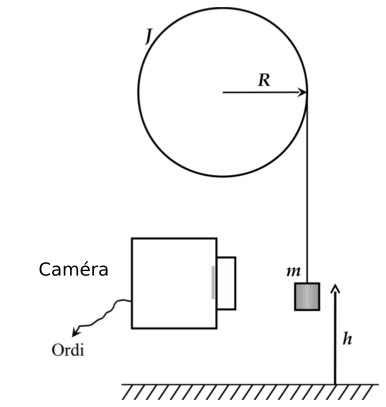
\includegraphics[width=5cm]{images-exp/MecaCylindreTournant.png}}
 \caption{Expérience du cylindre tournant}
\end{figure}


Étude de la vitesse angulaire

    On note J le moment d'inertie du cylindre par rapport à son axe de rotation. Montrer qu'en l'absence de frottement la vitesse angulaire est de la forme :

    \[ \frac{\mathrm{d}\theta }{\mathrm{d}t} = \frac{g / R}{1 + J/mR^2} t + \mathrm{cste}\]

    Mesurer la vitesse v de la masse, tracer la courbe $v = f(t)$, et vérifier la loi ci-dessus. En déduire la valeur de $J$. On peut aussi intégrer une fois l'équation et tracer $h = f(t)$.

Conservation de l'énergie

L'énergie cinétique (proportionnelle à $v^2$) varie linéairement avec la hauteur de chute h. Le vérifier. Représenter l'énergie cinétique, l'énergie potentielle et l'énergie mécanique en fonction du temps. Vérifier la conservation de l'énergie mécanique. 

\subsection{Frottement solide, mouvement ralenti}
\underline{Références :}
\begin{itemize}
\item Bocquet, Faroux, Renault, Toute la mécanique (p 372)
\end{itemize}

Coefficient de frottement dynamique bois-bois, varier masse m2 et distance h

\begin{figure}
      \centerline{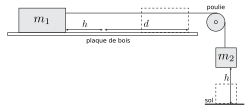
\includegraphics[width=5cm]{images-exp/Manip_frottement_solide.png}}
 \caption{Manip coefficient de frottement solide}
\end{figure}

La dynamique suivant le décrochage pour une masse $m_2$ supérieure à sa valeur critique renseigne sur le coefficient de frottement dynamique. La masse $m_2$ est lâchée sans vitesse initiale d'une hauteur h au dessus d'un obstacle qui limite sa chute (le sol par exemple). La masse $m_1$ parcourt une distance h+d sur le plan horizontal avant de s'arrêter. On peut relier le coefficient de frottement dynamique $f_d$ à $m_1$, $m_2$, $h$, et $d$ par la formule suivante (à savoir démontrer):

\[ f_d=\frac{m_2h}{m_2d+m_1(h+d)}\]

Faire varier $m_2$ en gardant $h$ et $m_1$ constantes, et tracer sur QtiPlot $m_2h$ en fonction de $m_2d+m_1(h+d)$, la pente correspondant à $f_d$. Comparer les valeurs trouvées pour $f_s$ et $f_d$ aux ordres de grandeurs usuels. 

\subsection{Rotation d'un solide : le gyroscope}
\underline{Références :}
\begin{itemize}
	\item Pérez, méca
\end{itemize}

Mesure de J

Préciser que les solides sont assimilés à des points

Le gyroscope permet d'observer le mouvement d'un solide S mobile autour d'un point fixe O. On étudie en particulier les mouvements obtenus lorsqu'il est initialement lancé dans une rotation très rapide ($\omega$) autour de son axe principal d'inertie OT.

Dans notre cas, le gyroscope S est constitué par l'ensemble suivant : disque de laiton de centre T + contrepoids C + axe de liaison. On notera $J$ le moment d'inertie du disque. Le mouvement autour d'un point fixe est réalisé à l'aide du cardan centré en O. 

\begin{figure}
      \centerline{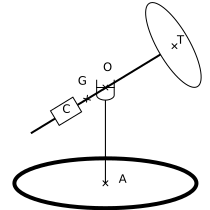
\includegraphics[width=5cm]{images-exp/MecaGyroscope.png}}
 \caption{Schéma d'un gyroscope}
\end{figure}

\section{Surfaces et interfaces.}

\underline{Références :}
\begin{itemize}
	\item Quaranta, méca
	\item Gouttes, bulles, perles et ondes
	\item hydro physique Guyon
	\item Sylvie Hénon – Bernard Cabannes (Belin)
\end{itemize}

\subsection{Interfaces statiques}
\subsubsection{Loi de Jurin}
Expérience avec les capillaires et l'éthanol
\begin{figure}
      \centerline{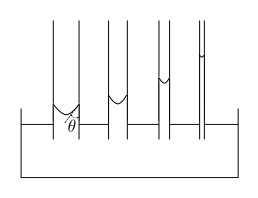
\includegraphics[width=5cm]{images-exp/Jurin1.png}}
 \caption{Montée du fluide dans les capillaires}
\end{figure}

Il s'agit de vérifier expérimentalement la loi de Jurin qui prévoit l'ascension des liquides dans les tubes capillaires.

Réaliser l'expérience avec de l'alcool, l'eau posant trop de problèmes de mouillage imparfait. On dispose de 4 tubes de diamètres différents. Avant de les immerger dans l'alcool, chasser tout liquide résiduel pour éviter la formation de bulles (pourquoi ?). Il est aussi possible de plonger les tubes dans la cuve et de faire couler de l'alcool dans les tubes grâce à une pipette en plastique. 
Faire l'image des tubes avec une lentille comme indiqué ci-dessous (attention, les images sont inversées sur l'écran !)


\begin{figure}
      \centerline{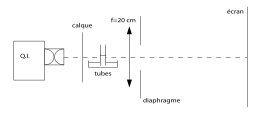
\includegraphics[width=5cm]{images-exp/Jurin2.png}}
 \caption{Montage pour projeter l'image des capillaires sur un écran}
\end{figure}

Tracer l'ascension h du liquide dans le tube en fonction du rayon r du tube. Cette hauteur h est la différence de hauteurs entre le ménisque dans le tube et la zone de la cuve où la surface du liquide est horizontale et plate (pourquoi ?). La relation théorique est : $h = 2 \gamma \cos \theta/ \rho g r$, où $\theta$ est l'angle de contact de l'alcool sur le verre. En déduire une estimation de $\gamma$ en prenant $\theta = 0$ (mouillage total du verre par l'alcool).

\subsubsection{Coefficient de frottement statique}
Bois-bois, plan incliné noter l'angle de début de glissement

Pour mesurer le coefficient de frottement statique, on dispose sur une planche de bois une masse $m_1$ composée d'un palet en bois sur lequel on dépose des masselotes supplémentaires afin de pouvoir diminuer la force normale en retirant ces masselotes ($m_1$ est la masse du palet et des masselotes posées dessus). En utilisant une poulie, on relie le palet par une ficelle à une autre masse $m_2$ (poids avec un crochet), voir schéma. En diminuant progressivement la masse $m_1$, on atteint une valeur seuil qui rompt l'équilibre, la condition $T<f_sN$, soit $m_2<f_sm_1$, n'étant alors plus vérifiée. On déduit $f_s$ de cette valeur critique de $m_1$. 

\subsection{Interfaces en mouvement}
\subsubsection{Coefficient de frottement dynamique}
Masse glisse sur planche attachée à un fil

cf plus haut

\subsubsection{Cuve à ondes}

\begin{figure}
	\centerline{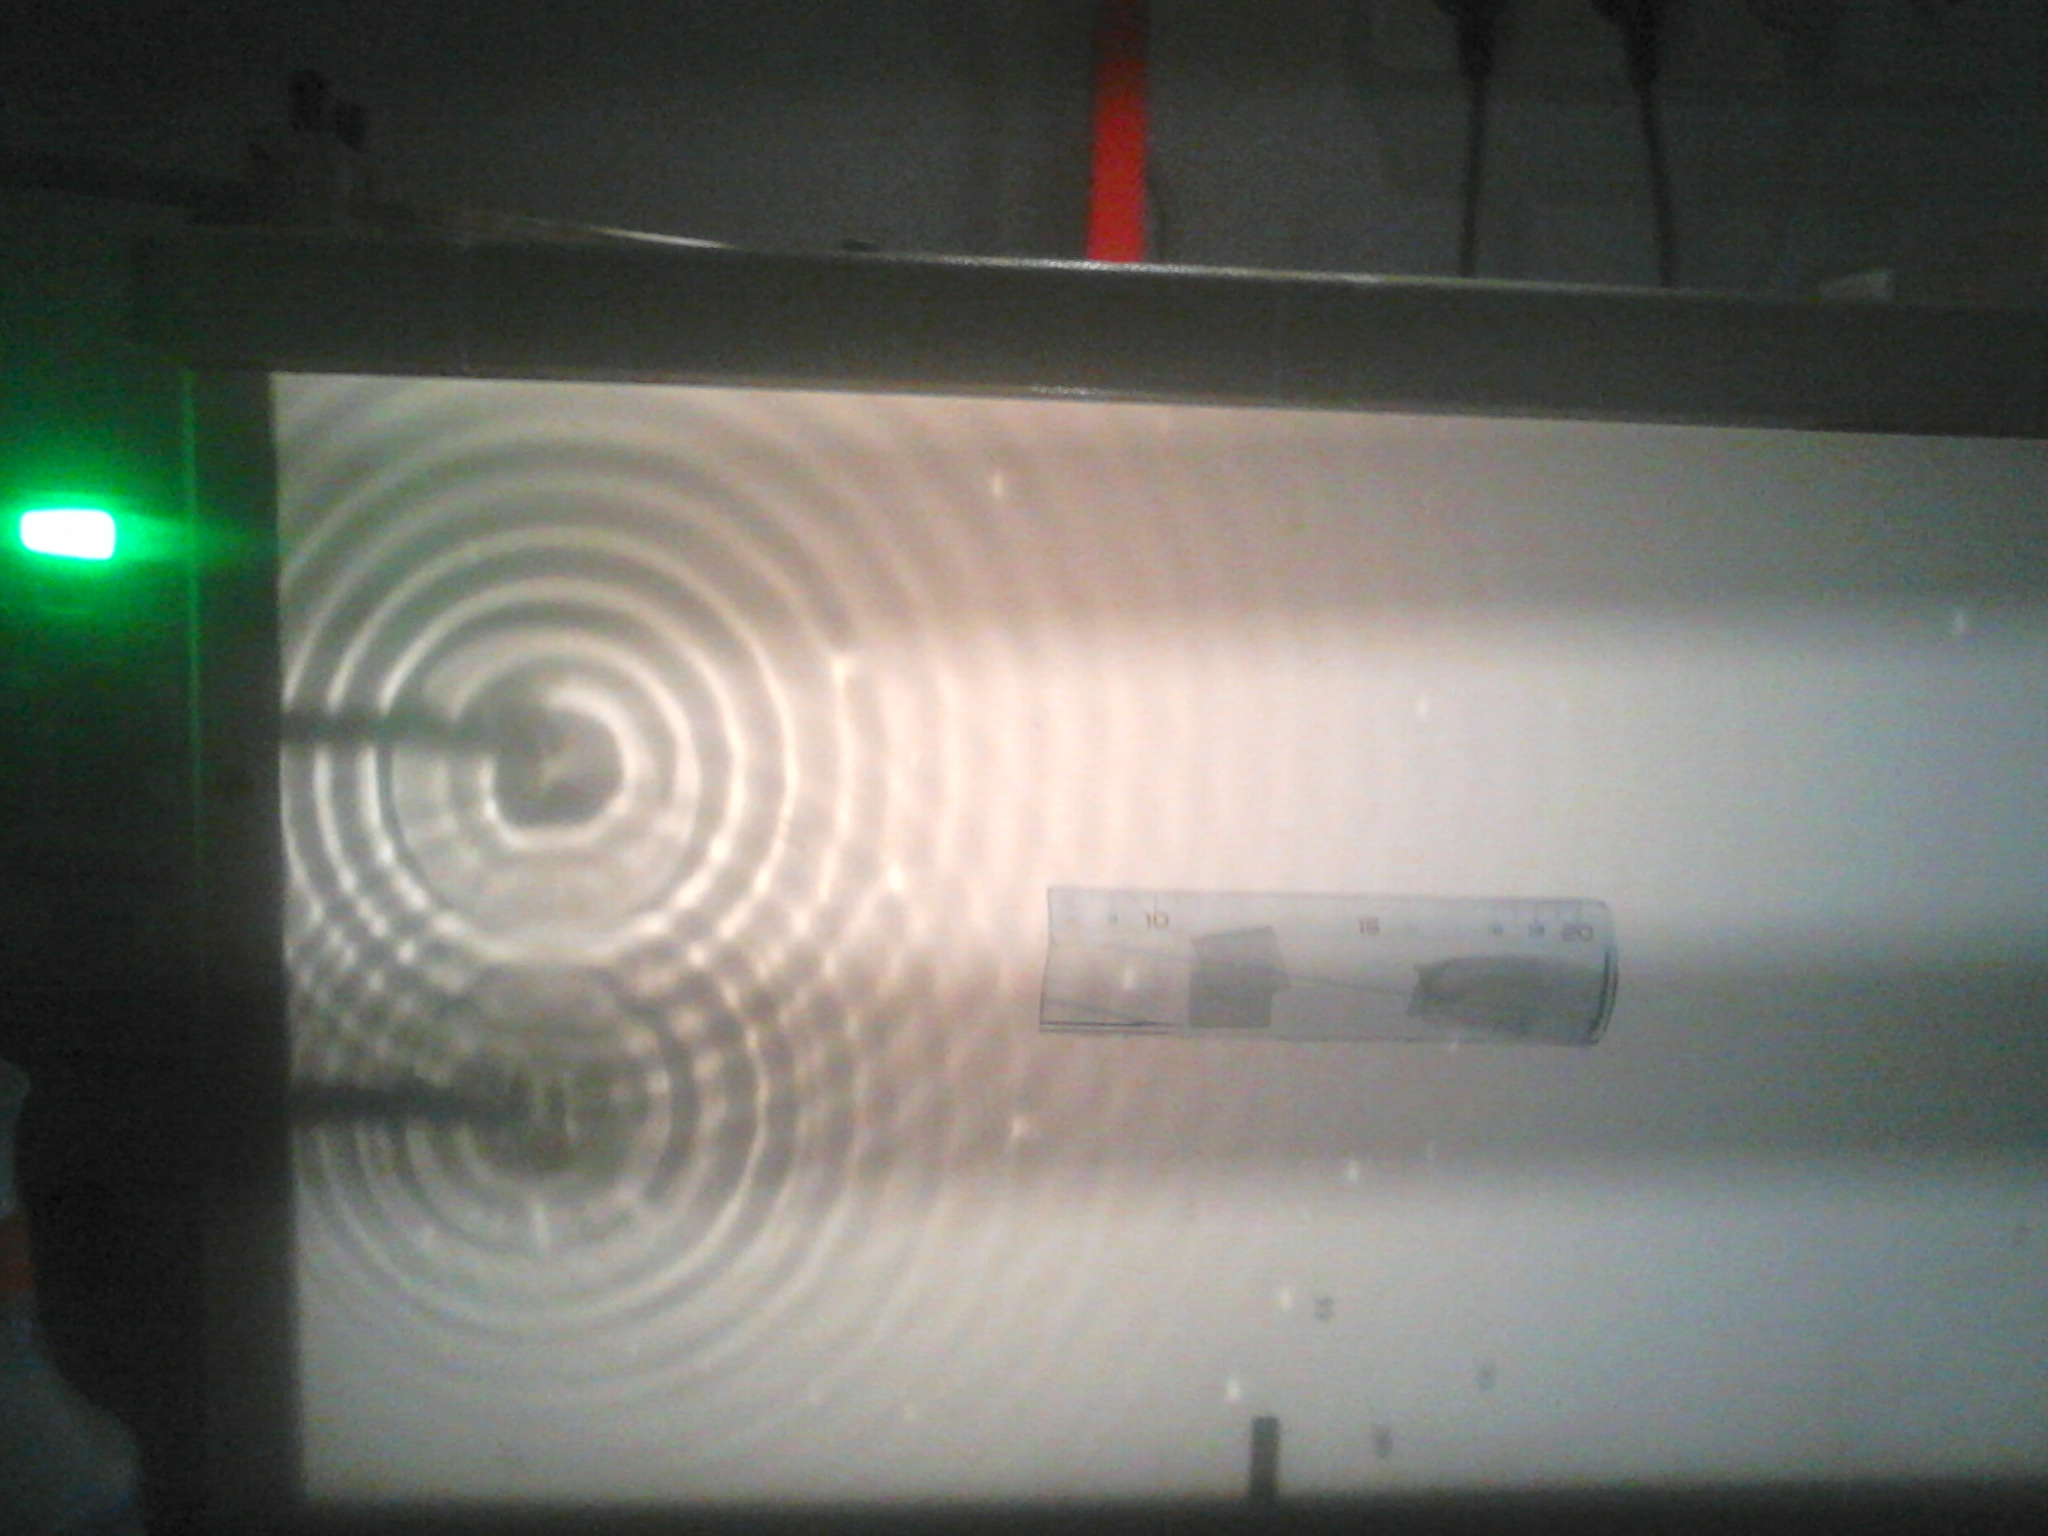
\includegraphics[width=5cm]{images-exp/cuve_ondes.jpg}}
 \caption{Expérience de la cuve à ondes}
\end{figure}
Utiliser la barrette pour générer des ondes planes. Rincer à l'avance à l'éthanol, évaporer avec un sèche-cheveux si besoin.

Relation de dispersion, en déduire $\gamma$

Lorsque la surface libre d'un liquide est perturbée, deux mécanismes physiques exercent un rappel vers l'horizontalité : la gravité, dont l'effet est caractérisé par la masse volumique du fluide $\rho$ et $g$ l'accélération de la pesanteur; et la capillarité caractérisée par la tension de surface $\gamma$. Pour des ondes de faible amplitude les équations et conditions aux limites peuvent être linéarisées et le calcul mène à la relation de dispersion suivante :

\[ \omega^2 =\tanh(kh) \left[ g k + \frac{\gamma}{\rho } k^{3} \right] \]

Deux cas limites apparaissent alors : pour les petites longueurs d'onde (k grand) le mécanisme de rappel dominant est la tension superficielle, alors que c'est la gravité qui domine quand la longueur d'onde est grande (k petit). On parlera respectivement d'ondes capillaires ou de gravité. L'échelle de longueur qui détermine le passage d'un régime à l'autre est la longueur capillaire $\sqrt{\gamma / \rho g}$. Elle est de l'ordre de quelques millimètres pour l'eau.


Pour réviser la théorie associée aux ondes de surface, vous pouvez utiliser avantageusement les références suivantes : l'ouvrage Hydrodynamique physique, E. Guyon, J.-P. Hulin, L. Petit ou, en ligne, le cours de M. Rabaud. 

Ce système est un des rares systèmes physiques disponibles à la collection permettant de générer des ondes dispersives et d'en mesurer la fréquence et la longueur d'onde. De ce fait, on devrait être en mesure de retrouver expérimentalement la relation de dispersion des ondes à la surface de l'eau précédemment rappelée. La notice de la cuve à onde (N614), est disponible en ligne.

Si $g$ et $\rho$ ne sont pas susceptibles de varier au cours de l'expérience il n'en est pas de même pour $\gamma$ qui peut être largement diminuée par la présence de graisses ou de surfactants dans la cuve. Ainsi, avant toute chose, vous devrez prendre soin de nettoyer soigneusement la cuve à onde à l'éthanol pour la dégraisser, à la laisser correctement sécher, et à utiliser de l'eau distillée dont la tension de surface est celle de l'eau pure : $\gamma \approx 70 $, $mN/m$ (à 20 degrés Celsius).

Vous pouvez dès lors préparer votre expérience :

    Remplir la cuve d'eau distillée sur une hauteur h de l'ordre du centimètre.
    Brancher, dans un premier temps, un unique point source à l'embout de la soufflerie via le tube en caoutchouc adapté. L'embout s'accroche au rail sur le côté de la cuve.
    Relier la fiche pour câble coax du générateur d'onde (ENSP4233) à un appareil permettant de mesurer la fréquence du signal, typiquement un oscilloscope. Celui-ci affichera la fréquence du jet d'air.

La déroulé de l'expérience est finalement le suivant : vous générez un flux d'air alternatif qui engendre des ondes propagatives à la surface de l'eau. Leur fréquence est mesurée à l'oscilloscope, et la longueur d'onde se mesure sur l'écran blanc face à la cuve en immobilisant l'image grâce au stroboscope. Attention à choisir judicieusement la méthode de mesure de la longueur d'onde, et à prendre garde au grossissement entre la taille réelle et la taille sur l'écran ! Estimer soigneusement les incertitudes et en déduire $k$ et $\omega$.

L'interprétation consiste à tracer les points expérimentaux $\omega$ en fonction de k puis, par un ajustement, à vérifier la relation de dispersion théorique et déterminer la tension de surface $\gamma$ de l'eau. Dans la pratique, on vérifiera que le terme $\tanh(kh)$ peut être approximé à l'unité. Il est également généralement plus simple d'ajuster par exemple $\omega^2/k$ en fonction de $k^2$, pour obtenir une droite de pente $\gamma/\rho$ et d'ordonnée g à l'origine.

Pour finir cette manip vous pouvez régler le stroboscope afin d'avoir une image parfaitement fixe, puis ajouter quelques gouttes de surfactants (typiquement du savon ou du liquide vaisselle). Vous observez le motif bouger, signe que la relation de dispersion a changé. Vous avez mis en évidence l'influence de la tension de surface sur la relation de dispersion. 

\section{Dynamique des fluides.}
\begin{itemize}
	\item hydro physique Guyon
\end{itemize}
\subsection{Chute dans le glycérol}

\begin{figure}
	\centerline{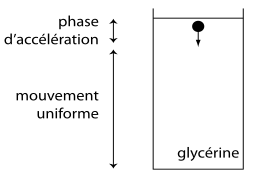
\includegraphics[width=5cm]{images-exp/chute_bille_glycerol.png}}
 \caption{Chute dans le glycérol}
\end{figure}

Attention, dévelloper la formule du coefficient de trainée au second ordre en $R_e$. Utiliser la caméra.

On définit le nombre de Reynolds de l'écoulement par $Re=2 R v \rho_\textrm{fluide}/ \eta$ , où $R$ est le rayon de la sphère, $v$ sa vitesse, $\rho_\textrm{fluide}$ la masse volumique du fluide et $\eta$ sa viscosité. En régime visqueux, i.e. $Re < 1$ la force de traînée s'exerçant sur la sphère vaut $F = -6\pi\eta R v$ .

L'expérience proposée vise à vérifier la loi de Stokes, et à mesurer la viscosité de la glycérine. 

On laisse tomber une bille d'acier. Quand le mouvement est uniforme (la phase d'accélération est liée à l'inertie de la bille, à l'inertie du fluide qui rajoute un terme de masse ajoutée et aussi au fait que la bille se trouve près d'une surface libre, si on la lâche à proximité de la surface air/glycérol. Il est recommandé de ne pas discuter cette phase d'accélération en montage.), on mesure la vitesse v en prenant le temps que la bille met à parcourir une distance fixée au préalable. Répéter l'expérience avec des billes de différents rayons R. On pourra mesurer la vitesse moyenne de chute entre deux points à l'aide d'un chronomètre. Une autre solution est d'utiliser la caméra rapide Jeulin et le logiciel Cinéris. Dans ce cas, il convient d'utiliser la caméra en mode rapide, et de veiller à éclairer fortement la zone filmée (sans chauffer le glycérol, utiliser par exemple un panneau lumineux placé derrière le cylindre), afin d'assurer un bon contraste entre la bille et le fond. Il est également nécessaire que le diamètre de la bille soit suffisamment grand (5 pixels ou plus).

Tracer $v_{\textrm{limite}}$ en fonction de R, et déterminer $\eta$ en ajustant vos résultats par la loi de Stokes. Pour quelles valeurs de R la loi de Stokes est-elle vérifiée ? Est-ce cohérent avec la valeur (à calculer) des nombres de Reynolds ?

\subsection{Ecoulement de Poiseuille}
Peser l'éprouvette pour calculer le flux. Attention aux niveaux du tube dans le vase source et du robinet de sortie (fixent la pression à la pression atmosphérique).

\begin{figure}
	\centerline{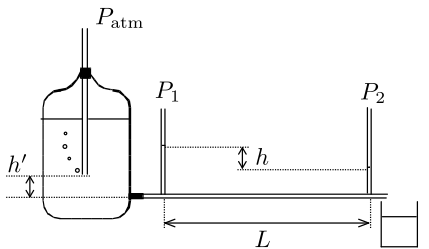
\includegraphics[width=5cm]{images-exp/EcoulementPoiseuille.png}}
 \caption{Ecoulement de Poiseuille}
\end{figure}
On veut vérifier la loi de Poiseuille qui donne le débit volumique Q de l'écoulement en fonction du gradient de pression $\frac{\Delta P}{L}$ mesurée entre deux points de l'écoulement, dans le cas du tube cylindrique :

\[ Q = \frac{\pi r^4 \Delta P}{8 \eta L}\]

où $\eta$ est la viscosité dynamique de l'eau, r le rayon et L la longueur du tube. Cette loi est valable en régime visqueux et elle correspond à un champ de vitesse parallèle à l'axe du tube dont la norme suit un profil parabolique. Suffisamment loin du début du tube, cette loi reste valable jusqu'à des nombres de Reynolds $Re=2 r U \rho/ \eta$ de l'ordre de 2000 (cette valeur ne correspond pas à une instabilité linéaire de l'écoulement, l'écoulement est instable vis-à-vis de perturbations d'amplitude finies. La gamme d'observation du régime de Poiseuille dépend du soin apporté à l'expérience.), où $U$ est la vitesse moyenne dans le tube. La validité de la loi de Poiseuille pour des nombres de Reynolds nettement supérieurs à 1 vient du fait que la solution de Poiseuille annule exactement le terme non linéaire de l'équation de Navier-Stokes ($\mathbf{v}\cdot\mathbf{grad})\mathbf{v}$), et que cette solution reste solution de l'équation de Navier-Stokes pour un nombre de Reynolds quelconque.

La surpression dans le tube est imposée en ajustant la hauteur du tube inséré dans la bouteille. La hauteur {h}', légèrement supérieure à $h$, donne la différence de pression entre les deux extrémités du tube. Cependant, l'étude de l'écoulement est faite entre les deux dérivations, à l'endroit où le régime de Poiseuille est bien établi. Nous mesurerons $\Delta P = P_1 - P_2 = \rho g h$ (Si le long tube n'est pas tout à fait horizontal, il peut y avoir $h\neq 0$ sans écoulement ; il faut alors corriger cette erreur systématique.) à l'aide de papier millimétré. Pour mesurer le débit, utiliser un chronomètre et un bécher ou une éprouvette graduée de 40-50 ml. Attendre que le régime soit permanent.

Calculer les nombres de Reynolds associés à l'écoulement. Vérifier que, dans une gamme où le débit est suffisamment faible, Q est effectivement proportionnel à h et en déduire la viscosité $\eta$ de l'eau. Comparer aux valeurs tabulées dans le Handbook (la viscosité de l'eau dépend notablement de la température). 


\subsection{Tube de Pitot}
A retravailler, parler de fluides parfait et de la loi de Bernouilli

Dans un écoulement parfait et incompressible (à quelles conditions sont valables ces approximations? voir notamment Guyon, Hulin, Petit, 2e édition p. 139 pour la condition d'incompressibilité), on a le long d'une ligne de courant :

\[ \frac{1}{2} v^{2 } + g z + \frac{p}{\rho} = C_{ste}\]

Le tube de Pitot est un tube double : 
\begin{figure}
	\centerline{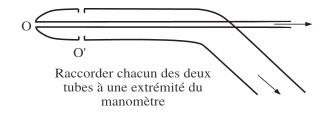
\includegraphics[width=5cm]{images-exp/Pitot.png}}
	\caption{Tube de Pitot}
\end{figure}
\begin{itemize}
\item Utiliser la grosse soufflerie.
\item La différence entre les pressions en O et O' donne accès à la vitesse en O' (établir la relation). Pour mesurer cette différence de pression, on utilisera le capteur prévu à cet effet, en branchant chacun des deux tubes à un embout du boitier. Le capteur délivre un signal de tension continu, linéaire en fonction de $\Delta P$.
\item Il faut faire attention à la position du tube, car il donne une valeur locale de la vitesse.
\item Utiliser aussi l'anémomètre à fil chaud à affichage numérique et le débimètre à hélice, afin de mesurer v et de tracer la courbe $\Delta P(v)$.
\end{itemize}

\section{Capteurs de grandeurs mécaniques.}
\subsection{Position}
\subsubsection{Capteur capacitif de niveau d'eau}
Même manip que pour effets capacitif. Marche bien. Faire l'étalonnage.

La mesure du niveau d'un liquide contenu dans une cuve opaque peut être réalisée à l'aide de capteurs capacitifs. Deux cas sont à envisager selon que le liquide est électriquement isolant ou conducteur. Dans le cas d'un liquide isolant la variation de capacité est due au changement de diélectrique dans le condensateur formé de deux conducteurs métalliques. Dans le cas d'un liquide conducteur, le condensateur est constitué d'un conducteur recouvert d'une fine couche d'un matériau isolant (diélectrique); le liquide joue alors le rôle de la seconde armature du condensateur. La variation de capacité résulte alors du changement de l'aire des armatures du condensateur.

La capacité $C$ varie linéairement avec la hauteur de liquide $h$. La capacité $C_{0}$ est la capacité du condensateur en l'absence de liquide. La pente dépend de la permittivité du vide $\epsilon_{0}$, de la constante diélectrique $\epsilon_{r}$ du matériau isolant et de la géométrie (plane ou cylindrique) du capteur.

Dans la pratique, la géométrie cylindrique est la plus simple à mettre en oeuvre et permet de minimiser les effets de bord. Pour les liquides isolants, une tige conductrice cylindrique est introduite dans la cuve qui constitue souvent la seconde armature du condensateur. Pour les liquides conducteurs, une tige conductrice et cylindrique, recouverte d'une couche d'un matériau isolant, est introduite dans la cuve. Un second conducteur est plongé dans le liquide (seconde armature du condensateur) pour permettre la mesure de capacité.

Enfin, dans le cas d'un liquide isolant, la capacité risque d'être très faible (e est grand) et les effets de bords importants surtout si la cuve sert d'armature. Le capteur est alors utilisé comme détecteur de niveau en "tout ou rien". On détecte alors seulement une variation de capacité quand la sonde plonge dans le liquide isolant. Le capteur n'a donc pas besoin d'être linéaire. 

Comportement électrique de l'eau
\begin{figure}
	\centerline{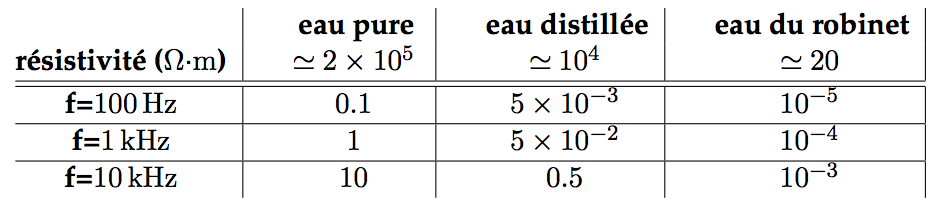
\includegraphics[width=5cm]{images-exp/Tableau_resistivite_eau.png}}
	\caption{Résistance de l'eau}
\end{figure}

On considère un condensateur formé de deux conducteurs de surface S séparés par une épaisseur d'eau $e_{eau}$. Un tel condensateur est caractérisé par sa résistance $R_{eau}$ en parallèle avec son impédance capacitive $\frac{1}{jC_{eau}\omega}$, où $C_{eau}$ et $\omega$ sont la capacité et la pulsation, respectivement. Le rapport de ces deux impédances vaut en module (On peut montrer que $a=\rho \epsilon_{0}\epsilon_{eau} \omega$ reste significatif indépendamment de la géométrie du condensateur.)

$a=R_{eau}C_{eau}\omega=(\frac{\rho e_{eau}}{S})(\frac{\epsilon_{0}\epsilon_{eau}S}{e_{eau}})\omega=\rho \epsilon_{0}\epsilon_{eau} \omega$, avec $\epsilon_{0}$ et $\epsilon_{eau}$ les permittivités du vide et de l'eau.

Si $a\ll 1$ le dipôle se comporte comme une résistance pure $R_{eau}$. Si $a\gg 1$ le dipôle se comporte comme un condensateur de capacité $C_{eau}$.

Le tableau ci-dessous présente l'ordre de grandeur attendu pour le coefficient $a=\rho \epsilon_{0}\epsilon_{eau}$ $\omega$ pour de l'eau contenant plus ou moins d'espèces dissoutes : eau pure, eau distillée (à l'abri du $CO_{2}$) et eau du robinet. Les fréquences de test envisagées (100 Hz, 1 kHz et 10 kHz) sont celles généralement disponible sur les RLC-mètres. 

Le comportement capacitif est observé pour les valeurs de résistivité et de fréquences élevées. Le comportement résistif (c'est à dire conducteur) est observé pour les faibles valeurs de résistivité et de fréquence.

Dans la suite, on suppose que l'eau a un comportement totalement résistif (ou de façon équivalente que l'eau est un liquide conducteur).
Manipulation
Description du dispositif
\begin{figure}
	\centerline{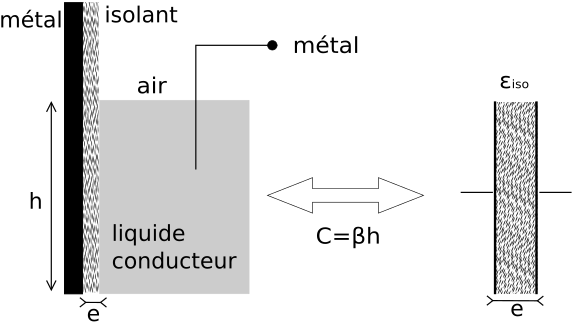
\includegraphics[width=5cm]{images-exp/NiveauCapa-liqcon.png}}
	\caption{Capteur de niveau capacitif, liquide conducteur}
\end{figure}
\begin{figure}
	\centerline{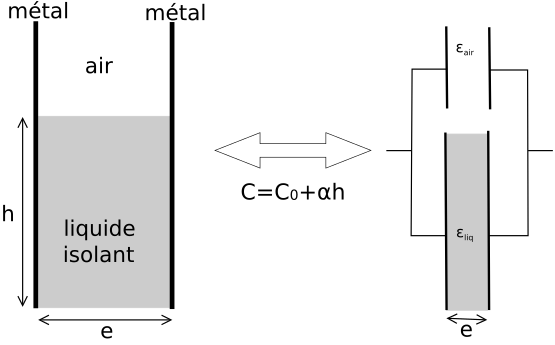
\includegraphics[width=5cm]{images-exp/NiveauCapa-liqiso.png}}
	\caption{Capteur de niveau capacitif, liquide isolant}
\end{figure}

La sonde capacitive est constituée d'un fil de cuivre verni. Ce fil verni est courbé de façon à former un "U", l'extrémité du coeur en cuivre n'est donc pas en contact avec l'eau. Un second fil de même nature et dénudé permet d'établir un contact électrique avec l'eau. L'ensemble est protégé par un tube transparent en PMMA[2]. Une bande millimétrée transparente est collée sur le tube pour permettre la lecture des variations de hauteur d'immersion de la sonde capacitive.
Utilisation

La sonde, tenue sur un support à l'aide d'une tige et d'une pince, est plongée dans un réservoir contenant de l'eau du robinet. Le niveau d'immersion est contrôlé en modifiant la hauteur du support ou en vidant le récipient progressivement avec un siphon (utiliser une pince à clamper pour déclencher et interrompre la vidange). Mesurer la capacité de la sonde à l'aide d'un RLC-mètre en fonction de la profondeur d'immersion. Pour améliorer la précision de la mesure, on peut utiliser des câbles BNC banane-banane sur les entrées + et -, et relier les masses de ces câbles BNC à la borne de garde du RLC-mètre. On peut réaliser un étalonnage, et chercher ensuite à déterminer une hauteur inconnue. On peut aussi déduire des résultats obtenus l'épaisseur de la couche de vernis recouvrant le fil de cuivre.

Pour aller plus loin, consulter la notice N.197. 

\subsection{Vitesse : mesure par effet Doppler}

On cherche à mettre en évidence l'effet Doppler. Pour cela, on utilise deux transducteurs piezoélectriques monté sur un banc à défilement : l'un est fixe et l'autre monté sur le support mobile du banc et se déplace, à vitesse constante, vers l'avant ou l'arrière. Régler la hauteur des transducteurs et adapter la fréquence d'excitation de sorte à avoir le signal le plus fort possible. Celle-ci doit se trouver autour de $f_{em}= 40 kHz$ mais elle peut varier de quelques centaines de Hertz. Lorsqu'on met en route la table traçante la fréquence $f_{rec}$ reçue par le transducteur mobile varie selon (le récepteur s'éloignant de l'émetteur) :
\[f_{rec} = \left(1 - \frac{v_{rec}}{c}\right) f_{em}\]

Étant donnée la faible vitesse de défilement (à mesurer avec précision), la différence de fréquences atteignable $\Delta f=f_{em}-f_{rec}$ est de l'ordre du hertz de sorte qu'une mesure directe de la fréquence ne sera pas assez précise pour distinguer $f_{em}$ de $f_{rec}$. On propose alors de réaliser une détection synchrone : l'idée est de multiplier le signal reçu de fréquence $f_{rec}$ par le signal émis de fréquence $f_{em}$ à l'aide d'un multiplieur. On obtient alors un signal modulé dont une décomposition en série de Fourier permet de se convaincre qu'il contient deux fréquences : $f_{rec}+f_{em}\approx 2f_{em}$ et $\Delta f$ qui ont des ordres de grandeur très différents. Un filtrage passe-bas effectué par un filtre RC en sortie du multiplieur permet de ne récupérer que le signal basse fréquence $\Delta f$ qui nous intéresse et dont on peut mesurer la fréquence précisément.

\begin{figure}
	\centerline{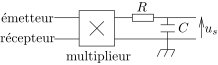
\includegraphics[width=5cm]{images-exp/CircuitEffetDoppler.png}}
	\caption{Circuit (demodulation+filtrage passe bas) pour la mesure de la vitesse par effet Doppler}
\end{figure}
Vous pouvez enfin confronter votre mesure de fréquence et sa précision à la valeur prévue par la formule théorique précédente à condition d'avoir rigoureusement mesuré la vitesse de défilement du banc. 

\subsection{Accéleration}
\begin{figure}
	\centerline{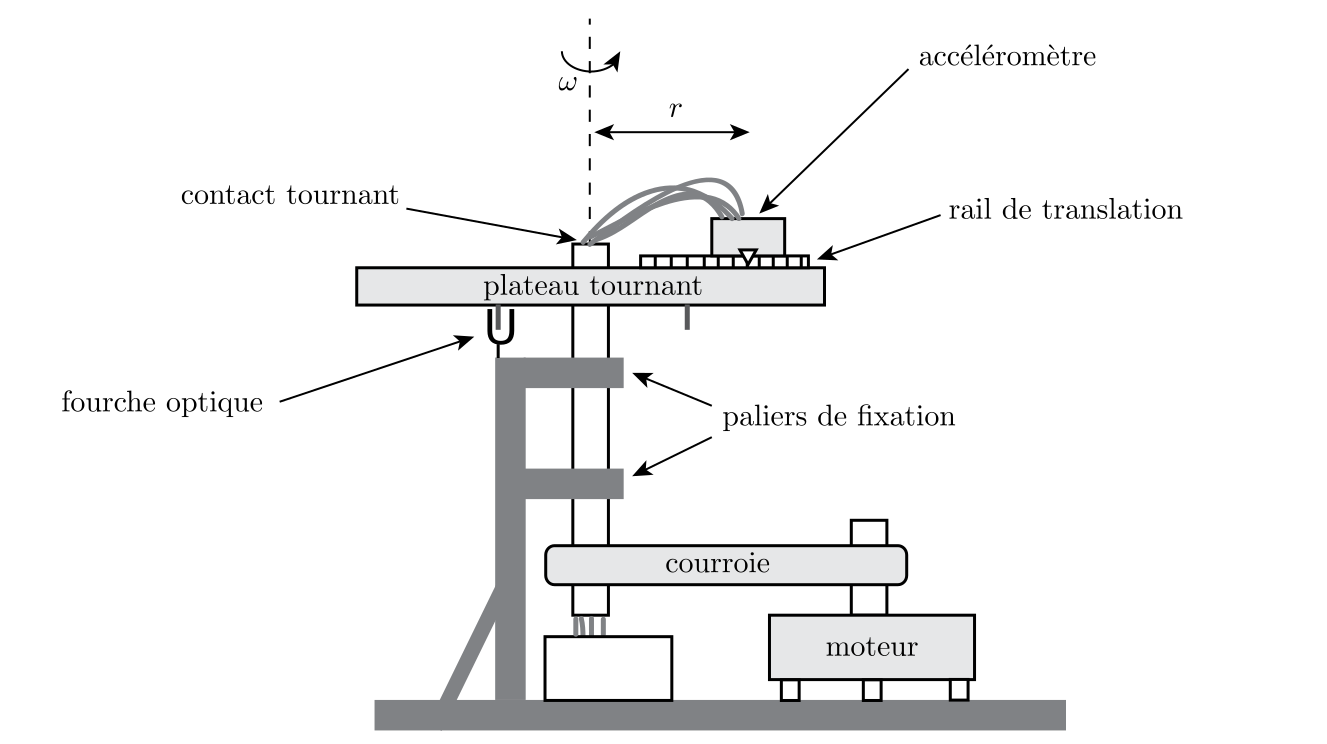
\includegraphics[width=5cm]{images-exp/Plateau_tournant.png}}
	\caption{Plateau tournant.}
\end{figure}

Accéléromètres

Il est indispensable de lire la notice, et en particulier la section Sécurité, avant d'utiliser ou de transporter l'expérience. Cette notice contient de plus des photos de l'expérience, et toutes les données nécessaires à son exploitation quantitative.
Principe

Un accéléromètre est un capteur permettant de mesurer des accélérations selon un ou plusieurs axes. Il peut être modélisé par un système masse-ressort, le déplacement de la masse par rapport à sa position d'équilibre étant proportionnel à l'accélération appliquée d'après le principe fondamental de la dynamique. Plusieurs types d'accéléromètres existent: asservis ou non asservis, et plusieurs formes de détection du mouvement de la masse peuvent être mises en oeuvre: détection capacitive, piézoélectrique, inductive, optique, etc.

On dispose d'un accéléromètre Analog Devices ADXL335 (à détection capacitive), capable de mesurer sur trois axes des accélérations comprises entre $3g$ et $-3g$. Ce capteur permet aussi bien de mesurer l'accélération statique de la gravité que de mesurer l'accélération dynamique résultant de mouvements, chocs ou vibrations.

L'accéléromètre est monté sur un plateau tournant, avec un de ses axes selon la direction radiale, de façon à pouvoir quantifier la force centrifuge liée à la rotation du plateau. 

Expérience

Consignes de sécurité :

le dispositif expérimental consiste en un plateau tournant, qui peut s'avérer dangereux. Il est impératif :

    de vérifier qu'il n'y a aucun objet mobile sur le plateau tournant.
    de vérifier qu'aucun fil ne gêne le mouvement du plateau, de la courroie ou du moteur.
    de vérifier que le chariot (situé sur le rail) est bien vissé, c'est-à-dire que la vis (Thorlabs) est vissée.
    de vérifier que le potentiomètre d'alimentation du moteur est au minimum.
    de vérifier que l'expérience est dans la boîte, et que celle-ci est bien fermée.

Le dispositif expérimental permet de comparer sans paramètre ajustable la force centrifuge à sa valeur théorique (à connaître). Cette expérience donne un accord quantitatif, si ce n'est pas le cas c'est qu'il y a un problème. Elle consiste en un plateau tournant, entraîné par un moteur à courant continu. La vitesse de rotation est mesurée grâce à une fourche optique. La force centrifuge est mesurée par un accéléromètre.

Moteur. Pour faire tourner le moteur, il est nécessaire d'utiliser une alimentation continue externe, non incluse dans le dispositif. Cette alimentation doit délivrer une tension de $12 V$, et doit pouvoir fournir une intensité de $5 A$. Le moteur est susceptible de ne pas fonctionner correctement si une alimentation moins puissante est utilisée. Par exemple, une alimentation ISO-TECH ENSP 4286 convient. Eteindre l'alimentation externe avant d'effectuer les branchements. Il faut ensuite brancher les sorties de l'alimentation externe sur les bornes rouge (positif) et noire (masse) du boîtier où se trouve le potentiomètre .

D'après les conseils de sécurité, le potentiomètre est initialement réglé au minimum. Il faut ensuite tourner progressivement le potentiomètre, pour augmenter la vitesse de rotation du plateau. Il est normal que la vitesse du plateau soit presque nulle sur une plage de valeurs du potentiomètre, puis qu'elle augmente rapidement.

Alimentation de la fourche optique et de l'accéléromètre La fourche optique et l'accéléromètre sont alimentés grâce à la prise à relier au secteur. Il faut ensuite que l'interrupteur situé sur la boîte près de l'axe de rotation soit sur la position 1.

Fourche optique La vitesse de rotation est obtenue à partir du signal de sortie de la fourche optique. Ce signal est obtenu à partir des sorties rouge et noire du boîtier noir situé près de l'axe de rotation. Il y a 2 vis sur le plateau tournant dont le passage à travers la fourche optique donne une impulsion de sortie. Pour mesurer la vitesse de rotation, il est conseillé d'utiliser un oscilloscope numérique et de mesurer soit avec des curseurs soit automatiquement le temps entre plusieurs impulsions. Il est conseillé de mesurer le temps qui correspond à un nombre entier de périodes de rotations parce que les temps entre deux impulsions successives (correspondant à des demi-rotations) ne sont pas tout à fait identiques à cause des imperfections du dispositif.

Rail La position de l'accéléromètre sur le plateau tournant peut être réglée à l'aide d'un rail de translation. La distance r entre le centre de l'accéléromètre et l'axe de rotation du plateau tournant est donnée par  : $r=l_0-l$ où $l_0=85 \pm 1 mm$ et où l est la position de la partie externe du chariot sur le rail. La valeur de l est la valeur en mm inscrite sur le rail de translation, en considérant la position de la face du chariot la plus éloignée de l'axe de rotation.

Il faut toujours visser correctement la vis Thorlabs du chariot avant de mettre en marche le moteur.

Accéléromètre L'accéléromètre se trouve dans la boîte grise. Un de ses axes est dirigé dans la direction radiale notée y , un autre dans la direction verticale notée z . Le troisième axe n'est pas utilisé.

Les sorties des signaux de l'accéléromètre sont situées sur la boîte noire située près de l'axe de rotation, sur la face opposée à celle où se trouve la sortie de la fourche optique. La tension $V_y$ , liée à l'accélération dans la direction radiale, est la tension entre l'embout bleu et la masse (embout noir). La tension $V_z$ , liée à l'accélération dans la direction verticale, est la tension entre l'embout jaune et la masse. Ces tensions sont typiquement de l'ordre de $2 V$ .

Le protocole expérimental consiste à mesurer les tensions $V_y(0Hz)$ et $V_z(0Hz)$ en l'absence de rotation (0 Hz). Ces mesures peuvent se faire à l'aide d'un voltmètre (par exemple les multimètres Agilent 34450A conviennent). Ensuite, il faut fixer une vitesse de rotation, et mesurer la tension $V_y$ en régime permanent.


La tension mesurée par les capteurs varie proportionnellement à l'accélération (tant que la tension à leur bornes est inférieure à la tension d'alimentation de l'accéléromètre). Le coefficient de proportionnalité dépend de la tension d'alimentation de l'accéléromètre. En l'absence de rotation, la différence entre les tensions $V_y(0Hz)$ et $V_z(0Hz)$ correspond à l'accélération $g$. L'accélération selon $y$ $a_y$ vaut donc :

$a_y=\frac{V_y-V_y(0Hz)}{V_z(0Hz) -V_y(0Hz)}g$

Les variations de $V_z$ avec la rotation sont dues aux imperfections du plateau tournant. 

\subsection{Jauge de contrainte}

Une jauge de contrainte est constituée d'un fil métallique ou semiconducteur très fin dont la résistance varie avec l'élongation. Collée directement sur une structure, elle en subit les déformations ; en ce sens, il s'agit plutôt d'une jauge de déformation.
\begin{figure}
	\centerline{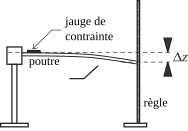
\includegraphics[width=5cm]{images-exp/JaugeContrainte.png}}
	\caption{Schéma du dispositif}
\end{figure}

La variation relative de sa résistance est donnée par :
\[ \frac{\Delta R}{R_0}= K \frac{\Delta l}{l_0}\]

où K est le facteur de jauge et $\Delta l/l_0$ est l'allongement relatif de la jauge.

La connaissance des propriétés élastiques de la structure permet de remonter aux contraintes appliquées. Une telle jauge est collée sur une poutre métallique encastrée à une extrémité.

Les lois de la résistance des matériaux montrent que l'allongement relatif de la jauge est relié au déplacement $ \Delta z$ de l'extrémité libre de la poutre par la relation (donnée dans la notice) :
\[ \frac{\Delta l}{l_0}= \frac{3e}{2 L^2}\Delta z \]

où L et e sont respectivement la longueur et l'épaisseur de la poutre ($e = 0,6 mm$).

\section{Mesure de température.}
Les capteurs en instrumentation industrielle, Asch et al.
\subsection{Etalonnage d'une sonde de platine}
Dans l'azote au point triple
(préparation à 77K, 273K, 373K)+fit

\begin{figure}
	\centerline{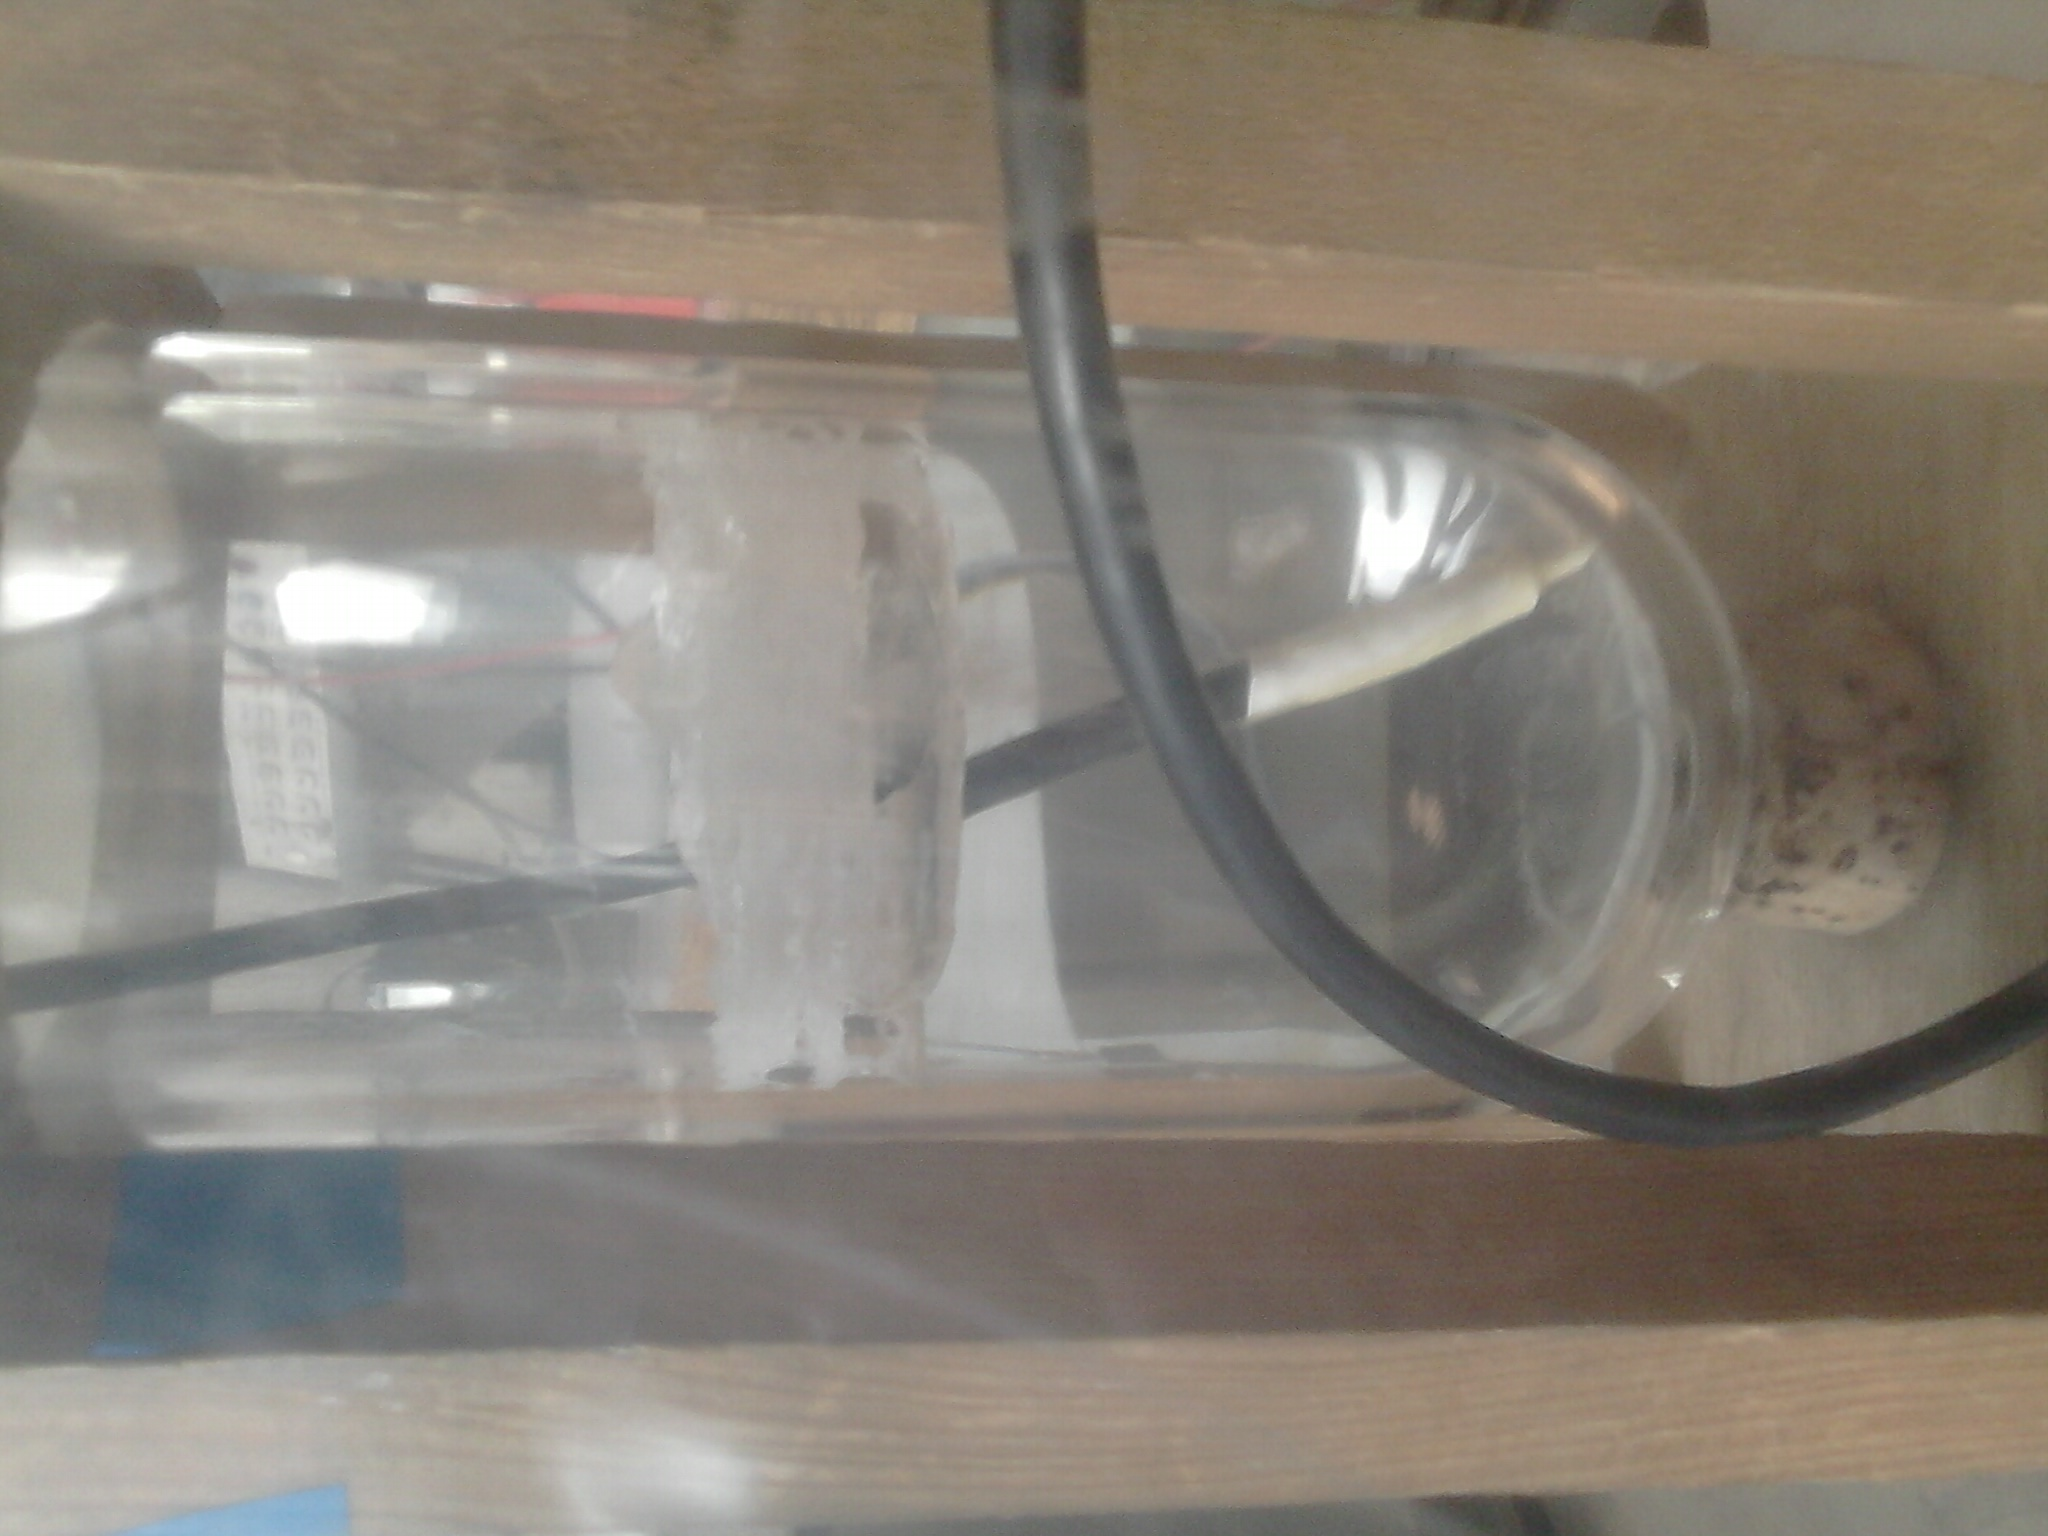
\includegraphics[width=5cm]{images-exp/pt_triple2.jpg}}
	\caption{Point triple de l'azote}
\end{figure}
\begin{figure}
	\centerline{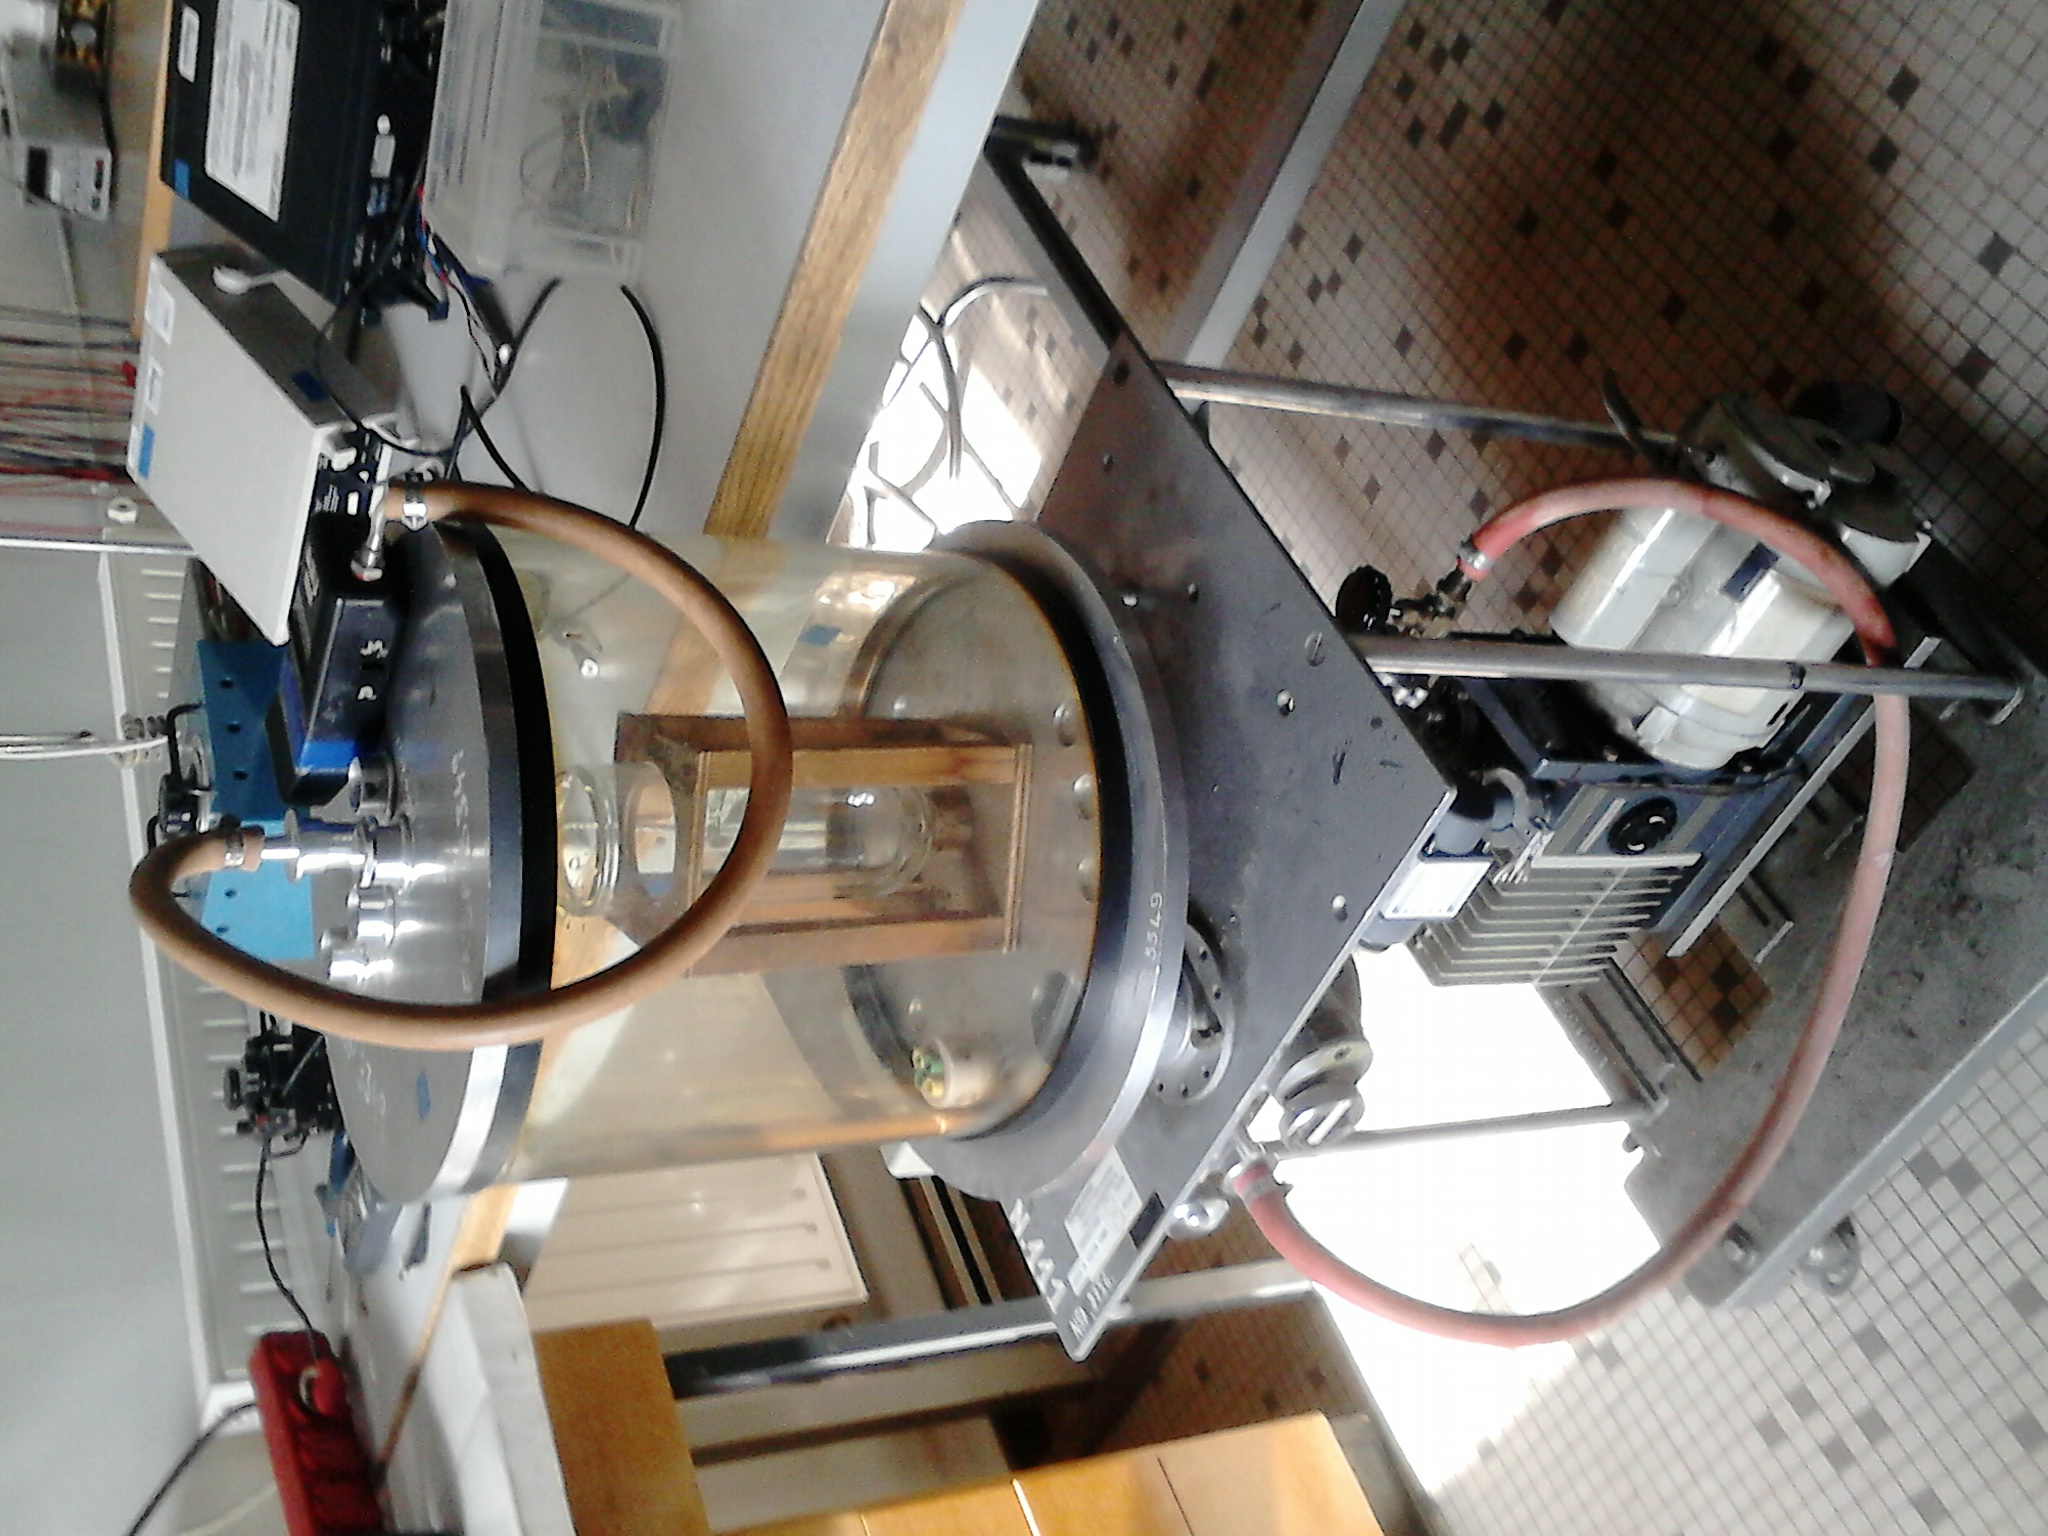
\includegraphics[width=5cm]{images-exp/cloche_vide.jpg}}
	\caption{Cloche à vide}
\end{figure}

Utilisée pour la définition de l'EIT-90, la sonde à résistance de platine permet également d'illustrer les précautions à prendre pour la thermométrie.

La sonde, fragile, est constituée d'un fil de platine très fin et calibré. On dispose en général d'une «Pt100» ( $R_{0} = 100 \Omega$ à $0^{\circ}\textrm{C}$) ou d'une «Pt1000» ($R_{0}=1000 \Omega$ à $0^{\circ}\textrm{C}$). La résistance de ce fil est tabulée en fonction de la température (cf. notice N455). La sonde est montée dans un support assurant un bon contact thermique avec le corps dont la température est à mesurer. Pour les expériences suivantes, on utilisera la sonde la plus robuste, montée dans un support en cuivre et en Teflon.

Il faut limiter le courant de mesure pour éviter d'abîmer la sonde (cf. notice pour la valeur du courant maximum), et pour perturber le moins possible la mesure à cause de l'auto-échauffement par effet Joule. On trouvera dans la notice la valeur du courant maximum, ainsi que le coefficient d'autoéchauffement permettant de faire les corrections éventuelles. Pour déterminer une température, mesurer la résistance $R_{0}$ dans le thermostat de référence (mélange eau-glace à $0^{\circ}\textrm{C}$) puis mesurer la résistance $R$ pour la température $T$ inconnue. Le rapport $R/R_{0}$ permet d'accéder à la température au moyen de la table ou de la formule donnée dans la notice.

La mesure de la résistance de la sonde se fait à l'aide d'une mesure quatre points (il faut être à l'aise sur son avantage par rapport à la mesure classique à deux points dite « courte dérivation »). On pourra

Utiliser pour cela la fonction quatre points des multimètres HP34401A (mode « $\Omega4W$»), (voir Métaux).

 Sinon appliquer une tension continue aux bornes de la sonde de platine, mesurer le courant avec un ampèremètre et la tension à ses bornes avec un voltmètre dans une configuration quatre points. Attention, afin de limiter le courant, il est important de placer une autre résistance R' en série avec la sonde.

La seconde méthode permet d'illustrer le phénomène d'autoéchauffement (facultatif) : mesurer la température de l'air ambiant, qui contrairement aux liquides évacue très mal la chaleur. Opérer avec une intensité assez élevée (pas trop, voir la notice). Mesurer la résistance juste après avoir établi le courant puis après avoir attendu le régime stationnaire, en utilisant un voltmètre résolvant $10 \mu V$. Évaluer l'écart de température, et la résistance thermique (en K/W) de cette sonde (et de son support) dans l'air. 

\subsection{Etalonnage d'une thermistance}
Avec la sonde de platine dans l'eau refroidissante, prendre les derniers points devant le jury

Un très grand nombre de thermomètres d'utilisation courante utilisent des thermistances comme capteur, car ils sont peu couteux et qu'un simple mesure de resistance permet d'obtenir une mesure de la température. Les thermistances sont des matériaux semi-conducteurs dont la résistance varie approximativement suivant la loi $R = A e^{B/ T}$

Il est facile de vérifier cette loi entre $0^\circ C$ et $100^\circ C$, par exemple avec de l'eau portée à ébullition qu'on laisse refroidir ; on relève alors la température à l'aide d'un des thermomètres précédent et la résistance de la thermistance (voir aussi le polycopié «semi-conducteurs» pour une autre vérification de cette loi). Cette étude peut aussi être l'occasion de faire quelques mesures de calorimétrie en mélangeant dans le calorimètre des masses différentes d'eau chaude et d'eau froide.

Elles sont aussi très utilisées dans les mesures de basses températures (on ne propose rien ici sur ce sujet) ainsi que dans les mesures courantes car elles ont une grande sensibilité.

La sensibilité est évaluée par le coefficient de température, défini par:
$\alpha = \frac{1}{R}\frac{dR}{dT}$


Le caractère exponentiel de la variation de la résistance de la thermistance en fonction de la température explique cette grande sensibilité. Cependant, la plage de température où celle-ci est valide est limitée, ce qui peut restreindre son utilisation. 

\subsection{Loi de Stefan, rayonnement du corps noir}
Pile de Moll à la sortie d'un four, fit log-log


\begin{figure}
	\centerline{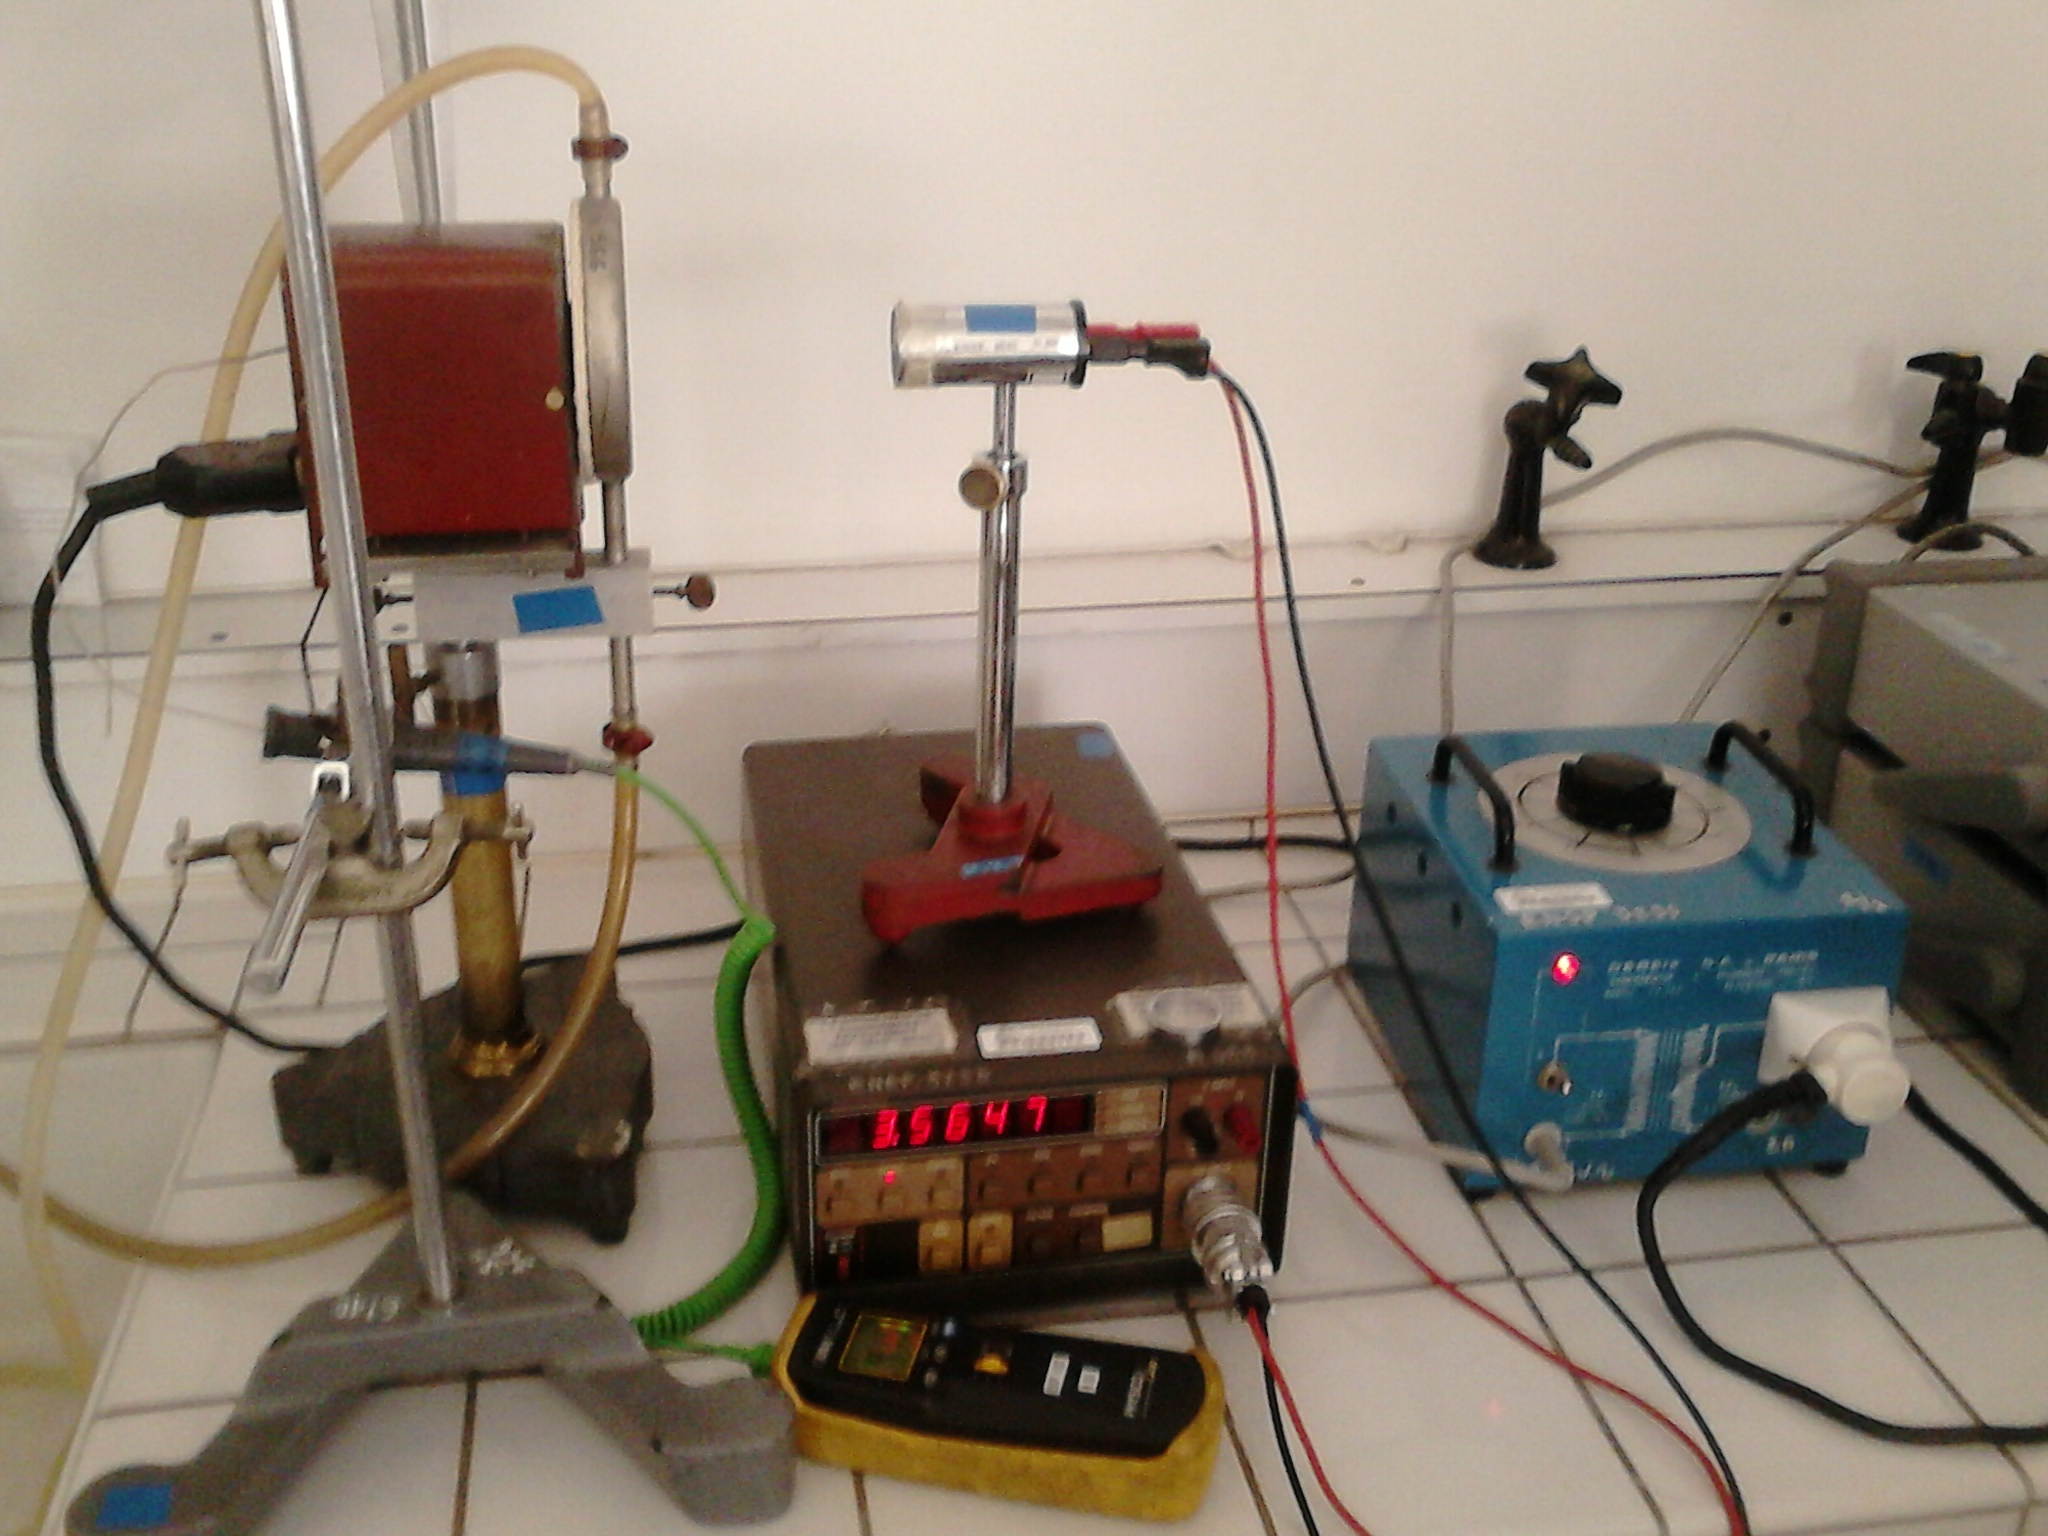
\includegraphics[width=5cm]{images-exp/pile_Moll.jpg}}
	\caption{Photo de l'expérience}
\end{figure}

À haute température, dans l'EIT-90, la température d'un corps noir est définie à l'aide de la formule reliant sa densité spectrale de luminance énergétique au voisinage d'une longueur d'onde laissée au choix de l'expérimentateur.

Par ailleurs, on peut utiliser des détecteurs infrarouges à large bande pour la réalisation pratique de l'EIT-90. On illustre ici le principe du «pyromètre à radiation totale» :
\begin{itemize}
\item pyromètre = instrument qui sert à mesurer les hautes températures;
\item à radiation totale: le détecteur est la thermopile, dont on aura ôté le filtre anti-thermique.
\end{itemize}
La thermopile est constituée par une succession de thermocouples, placés en série électriquement et en parallèle thermiquement, comme schématisé sur la figure 2.

\begin{figure}
	\centerline{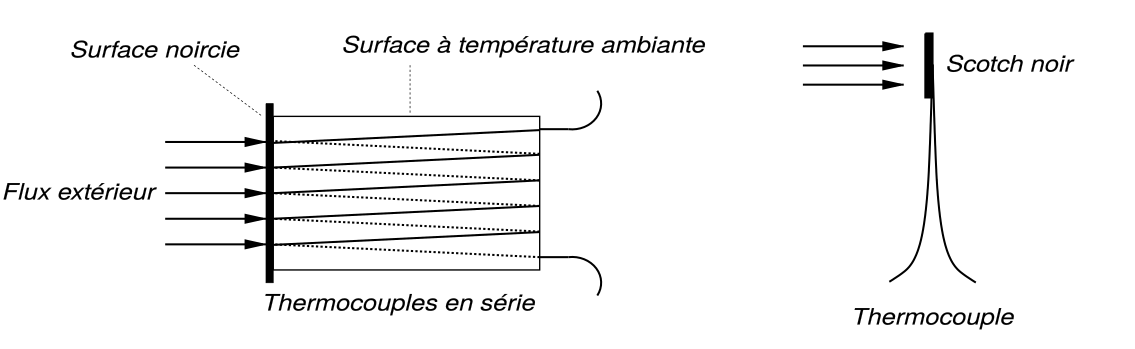
\includegraphics[width=5cm]{images-exp/ThermometriePrincipeThermopile_new.png}}
	\caption{Principe d'une thermopile}
\end{figure}

On propose d'effectuer ici une mesure relative de la température d'un corps noir (ce qui correspond aux techniques réelles) à l'aide du montage présenté figure 3. 

En pratique, on réalise un corps noir de la manière suivante : on utilise un four aux parois noircies percé d'une petite ouverture : tout rayon incident est piégé dans le four. A l'intérieur, le rayonnement est absorbé et réémis à plusieurs reprises par la paroi interne du four; une petite partie de ce rayonnement thermostaté est émise par l'orifice. Ce four est porté à la température $T$, son émission totale est donc proportionnelle à $T^4$ (loi de Stefan). On utilise un détecteur sensible au flux émis par le corps noir. Ce détecteur doit avoir une réponse spectrale plate, d'où le choix d'une thermopile.

Cette dernière mesure la différence de température $\Delta T_{\textrm{surf}}$ entre ses surfaces intérieures et extérieures. La température intérieure est $T_{\textrm{amb}}$. La surface extérieure chauffée par le flux $\Phi \propto T^4$ émis par le four chaud est à $T_{\textrm{amb}} + \Delta T_{\textrm{suf}}$. Alors, la réponse de la thermopile est de la forme :

\[V=\varepsilon \Delta T_{\textrm{surf}} = K(T^4-T_{\textrm{amb}}^4)\]

où $K$ est un facteur qui dépend de la sensibilité globale de la thermopile et de la géométrie de l'expérience, et qui est proportionnelle à la constante de Stefan $\sigma$.

\underline{En plus : schéma de principe d'un pyromètre optique}

\begin{figure}
	\centerline{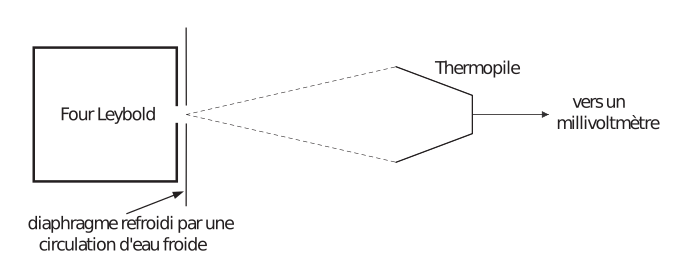
\includegraphics[width=5cm]{images-exp/ThermometriePrincipePyrometreOptique.png}}
	\caption{Principe d'un pyromètre optique}
\end{figure}
\section{Transitions de phase.}
\subsection{Transitions du premier ordre}

\subsubsection{Courbe de refroidissement de l'étain}

Monovariance d'un équilibre entre deux phases: équilibre solide-liquide pour l'étain, chaleur latente.

L'étain placé dans un creuset est chauffé à l'aide d'un bec Bunsen. Lorsqu'il est devenu liquide, éliminer la couche d'oxyde en surface, arrêter le chauffage et introduire un thermocouple prévu pour cet usage dans l'étain. Enregistrer sur LatisPro le refroidissement. En déduire la température de solidification de l'étain. Si l'étain est bien propre, on peut observer pendant la phase de refroidissement un retard au changement d'état. On aura intérêt à commencer l'enregistrement de la température dés le début du chauffage.

\begin{figure}
	\centerline{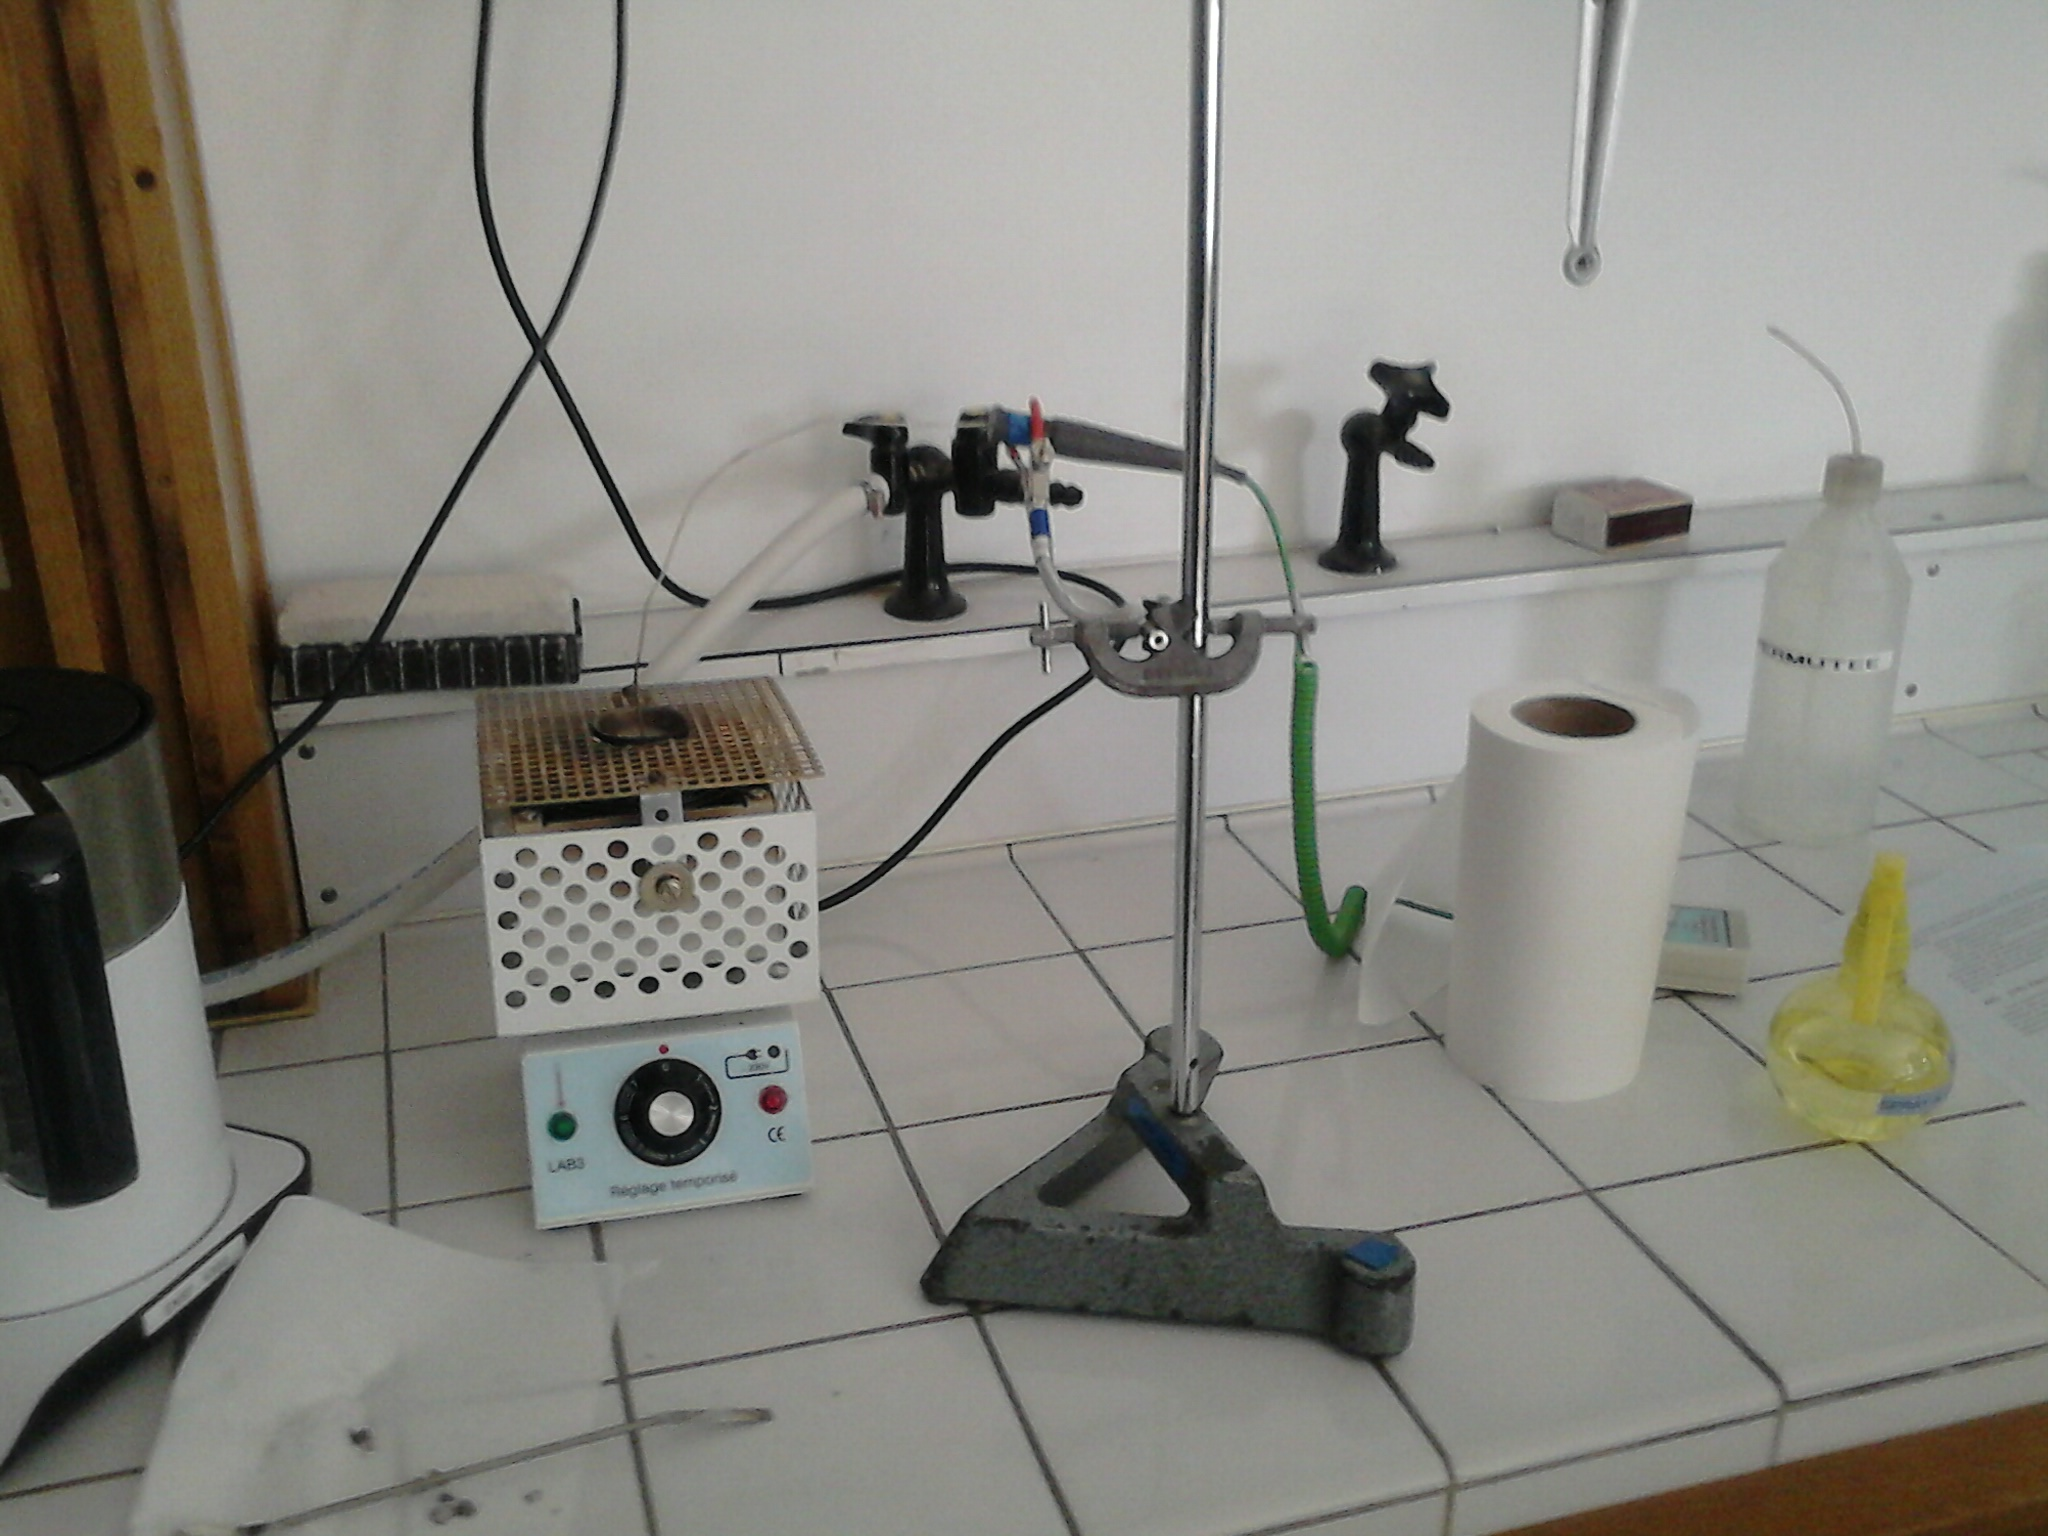
\includegraphics[width=5cm]{images-exp/transition_phase_Sn.jpg}}
	\caption{Courbe de refroidissement de l'étain : Photo du dispositif}
\end{figure}
Par définition, un changement d'état est du premier ordre s'il y a discontinuité d'au moins une des dérivées premières de l'enthalpie libre (ou du potentiel thermodynamque adapté au système étudié). Cela équivaut à l'existence d'une chaleur latente de changement d'état. On illustre ce cas en étudiant la vaporisation de l'azote.
Lancer au début + acquisition automatique (y revenir plus tard). Calculer la chaleur latente, on peut observer un petit pic dû à la surfusion.
\subsubsection{Diagramme P-V de SF6}
Premiers points vite, puis prendre son temps. Relevé d'un isoT devant le jury, les autres en prépation.

Le dispositif est constitué d'une éprouvette de verre graduée, verticale, contenant un fluide inerte (hexafluorure de souffre, SF6) que l'on comprime via un joint de mercure en tournant un volant.

\begin{figure}
	\centerline{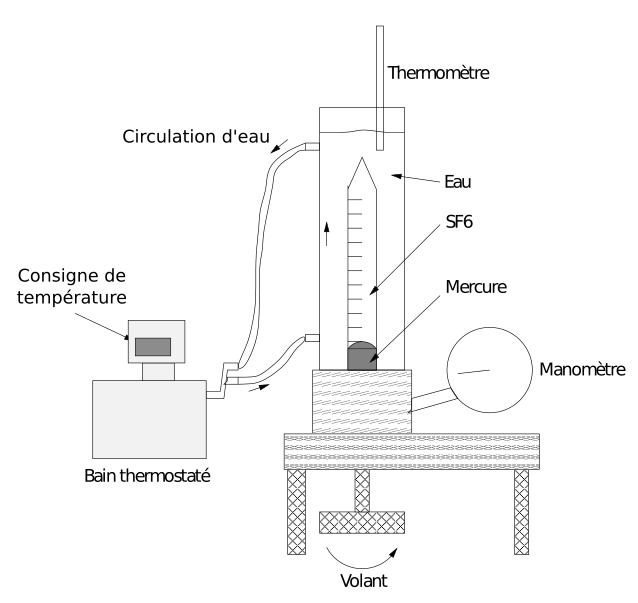
\includegraphics[width=5cm]{images-exp/IsoT_SF6.png}}
	\caption{Diagramme P-V de SF6 : Schéma du dispositif}
\end{figure}
\begin{figure}
	\centerline{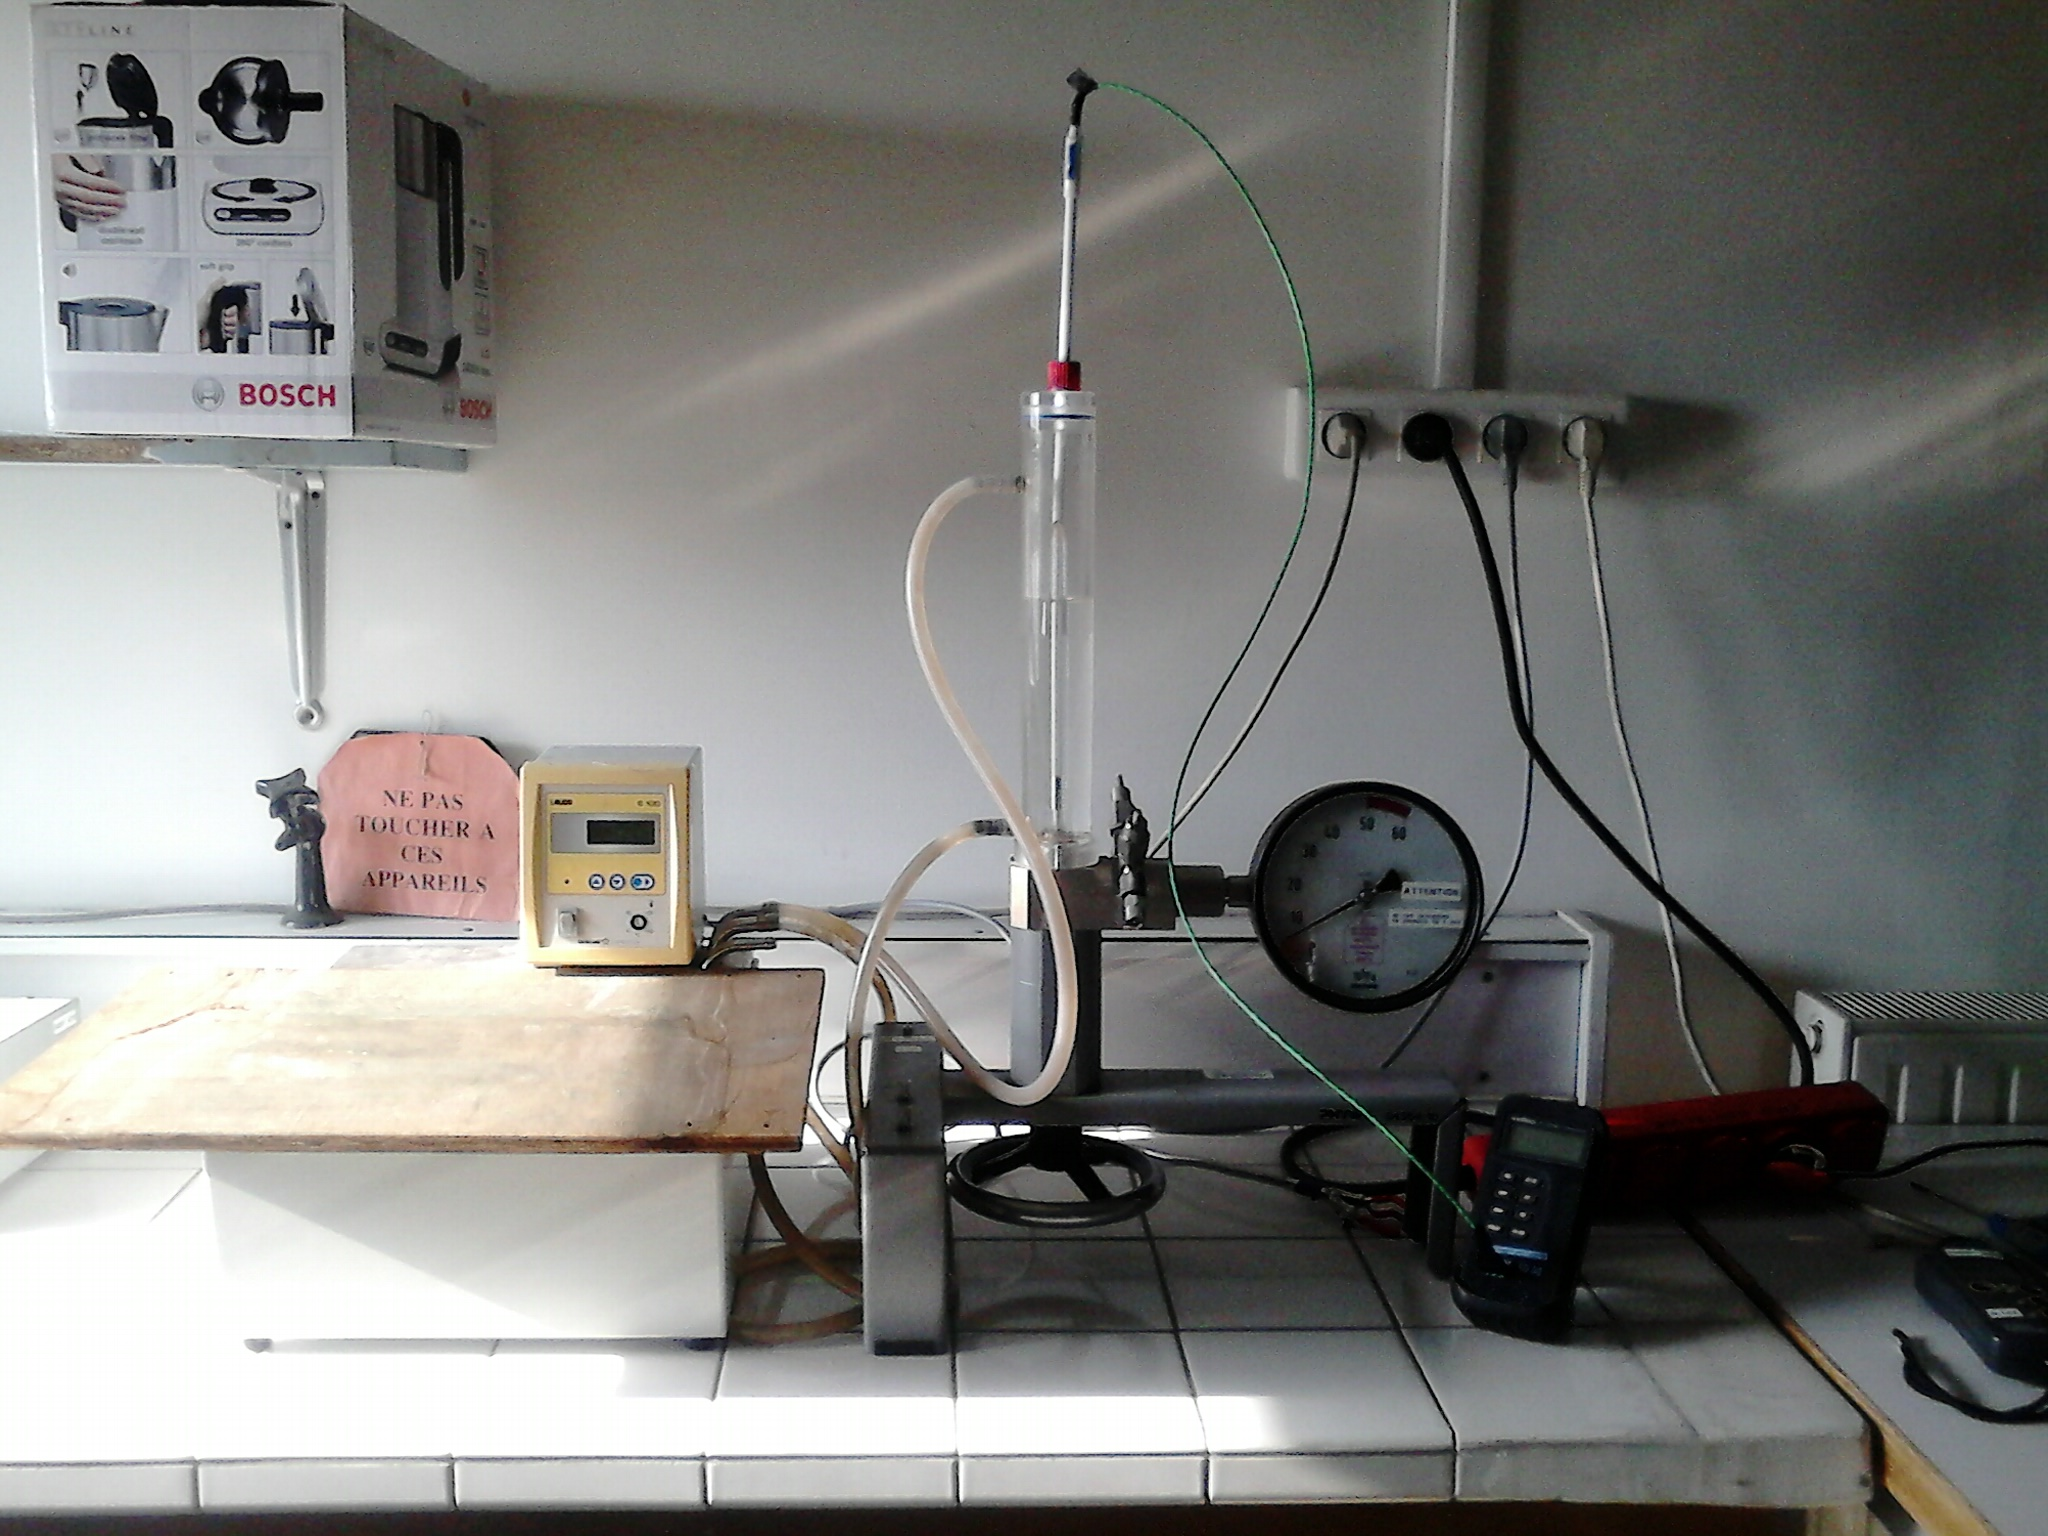
\includegraphics[width=5cm]{images-exp/diagramme_pv_sf6.jpg}}
	\caption{Diagramme P-V de SF6 : Photo du dispositif}
\end{figure}

On mesure le volume de SF6 en relevant la position du ménisque du mercure sous le SF6, par rapport aux graduations en mL de l'éprouvette. La pression imposée est lue en bar sur un manomètre incorporé. La pression maximale à ne pas dépasser est de 50 bars. L'éprouvette est elle-même contenue dans une contre-cuve en plexiglas, à travers laquelle on fait passer une circulation d'eau provenant d'un bain thermostaté. Par mesure de sécurité, il est indispensable, lorsqu'on comprime le SF6, que l'éprouvette soit entièrement recouverte d'eau. On impose la température par le bain thermostaté, dont la pompe permet de faire circuler l'eau à la température désirée dans la contre-cuve (consulter la notice). Il faut néanmoins un certain temps pour que l'éprouvette soit à la température de l'eau. La température est lue en degrés Celsius sur le bain thermostaté et est contrôlée sur un thermomètre au sommet de la contre-cuve. On fixe une température de consigne au bain thermostaté, puis on fait varier progressivement la pression et on relève le volume de SF6. La mise à l'équilibre est assez lente, compter environ 1 minute par degré d'écart. Essayer de faire des variations de faible amplitude et progressives. À partir d'une pression assez élevée, on observe la formation d'une interface liquide-vapeur, qui correspond à un palier de pression, c'est-à-dire une variation de volume à pression constante, par modification des proportions respectives de liquide et de gaz. On réitère l'opération pour plusieurs températures comprises entre la température ambiante et 50 °C.

On peut ainsi tracer les isothermes $P=f(V)$ du SF6 dans le diagramme de Clapeyron et caractériser une transition de phase du premier ordre. Les courbes de rosée et d'ébullition peuvent aussi être tracées. En utilisant la formule de Clapeyron, on peut déduire la chaleur latente de vaporisation du SF6. Dans la zone gazeuse, on peut montrer l'écart au gaz parfait, en traçant PV en fonction de $1/V$. Enfin, pour des températures au-dessus de 45 °C, on se trouve dans la zone de fluide supercritique et on peut essayer de contourner le point critique. L'observation du point critique semble par contre plus aisée dans la cellule scellée, à la densité critique (voir paragraphe suivant). Le point critique du SF6 est obtenu pour $T_\mathrm{crit}=45^{\circ} C$ et $P_{crit}=38 bars$.
Point critique: observation d'un point critique liquide-gaz

On dispose de cellules Leybold contenant de l'hexafluorure de soufre (SF6). Elles permettent de mettre en évidence quelques phénomènes physiques caractéristiques d'un point critique:
\begin{itemize}
	\item    disparition sur place du ménisque séparant les deux phases au point critique, lors du chauffage ;
	\item    coalescence, puis apparition d'un ménisque au milieu de la cellule après décantation, lors du refroidissement ;
	\item    opalescence critique au voisinage de $T_{c}$, très délicate à observer.
\end{itemize}
Fig. 5 Diagramme (p,V) d'un corps pur

Éclairer la cellule avec une lampe Quartz-Iode et un condenseur, projeter son image avec une lentille. Chauffer avec un sèche-cheveux.
\begin{figure}
	\centerline{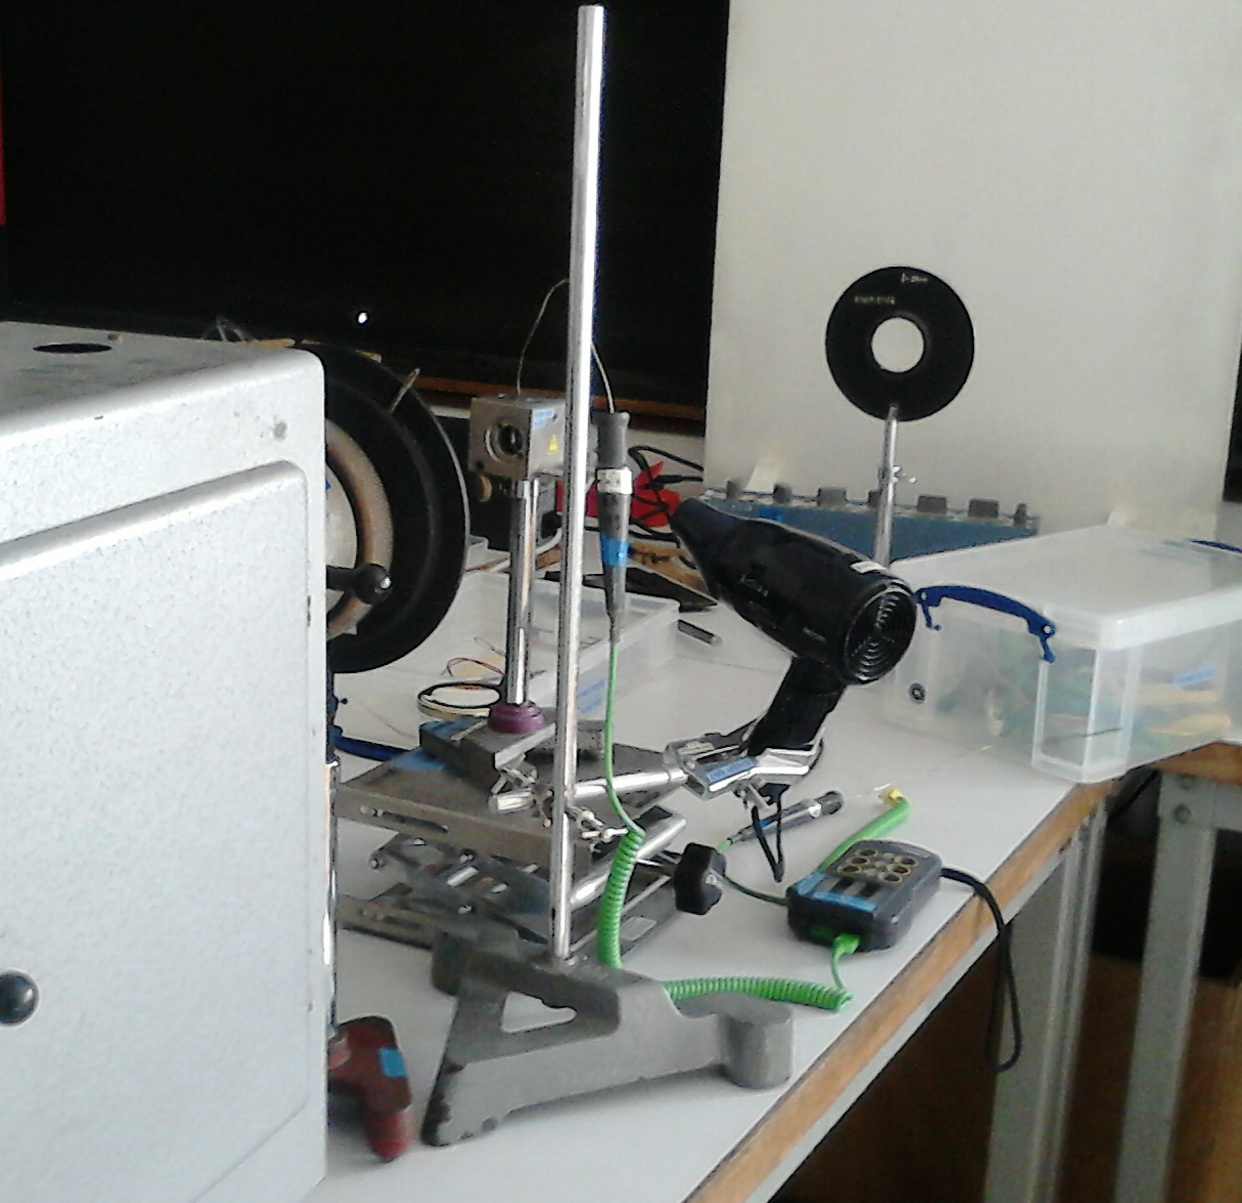
\includegraphics[width=5cm]{images-exp/opalescence_critique.jpg}}
	\caption{Opalescence critique de SF6 : Photo du dispositif}
\end{figure}

Observation et interprétation lors de la montée en température :

\begin{itemize}
	\item    Pour $T < T_{c}$ : Le ménisque s'élargit et devient de moins en moins net. Si l'on a une cellule remplie exactement à la densité critique, et une bonne régulation de température, on peut espérer observer l'opalescence critique. Près du point critique, la compressibilité du fluide diverge, et les fluctuations de densité, donc d'indice de réfraction, deviennent très grandes : cela provoque une diffusion importante de la lumière. La lumière diffusée prend une couleur bleue (intensité diffusée en $1/\lambda^{4}$) et la lumière transmise, initialement blanche, devient légèrement jaune.
	\item    Pour $T=T_{c}$: le ménisque disparaît car les deux phases deviennent identiques.
	\item    Pour $T > T_{c}$: une seule phase (fluide supercritique). La lumière transmise redevient progressivement blanche.
\end{itemize}

Lors de la descente en température

Lorsque T devient très légèrement inférieur à $T_{c}$, le système devient diphasique: apparition d'un brouillard dense formé par des gouttelettes des deux phases. Les gouttelettes d'une même phase coalescent et les phases liquide et vapeur se séparent nettement avec apparition d'un ménisque au milieu de la cellule. Le brouillard est, comme un nuage, opaque à la lumière : celle-ci ne traverse plus la cellule, qui prend une couleur gris-marron (phénomène à ne pas confondre avec l'opalescence critique).

Remarque : Pour une image plus spectaculaire, on peut utiliser un montage de strioscopie.


\subsection{Transition de phase du deuxième ordre}
\subsubsection{Transition ferromagnétique-paramagnétique}

Mesure de la température de Curie, transition ferromagnétique-paramagnétique du fer

À la température de Curie $T_C$, le fer passe de l'état ferromagnétique à paramagnétique. C'est une transition du second ordre: continuité des dérivées premières de l'enthalpie libre G, discontinuité des dérivées secondes, et donc absence de chaleur latente à la transition.
\begin{figure}
	\centerline{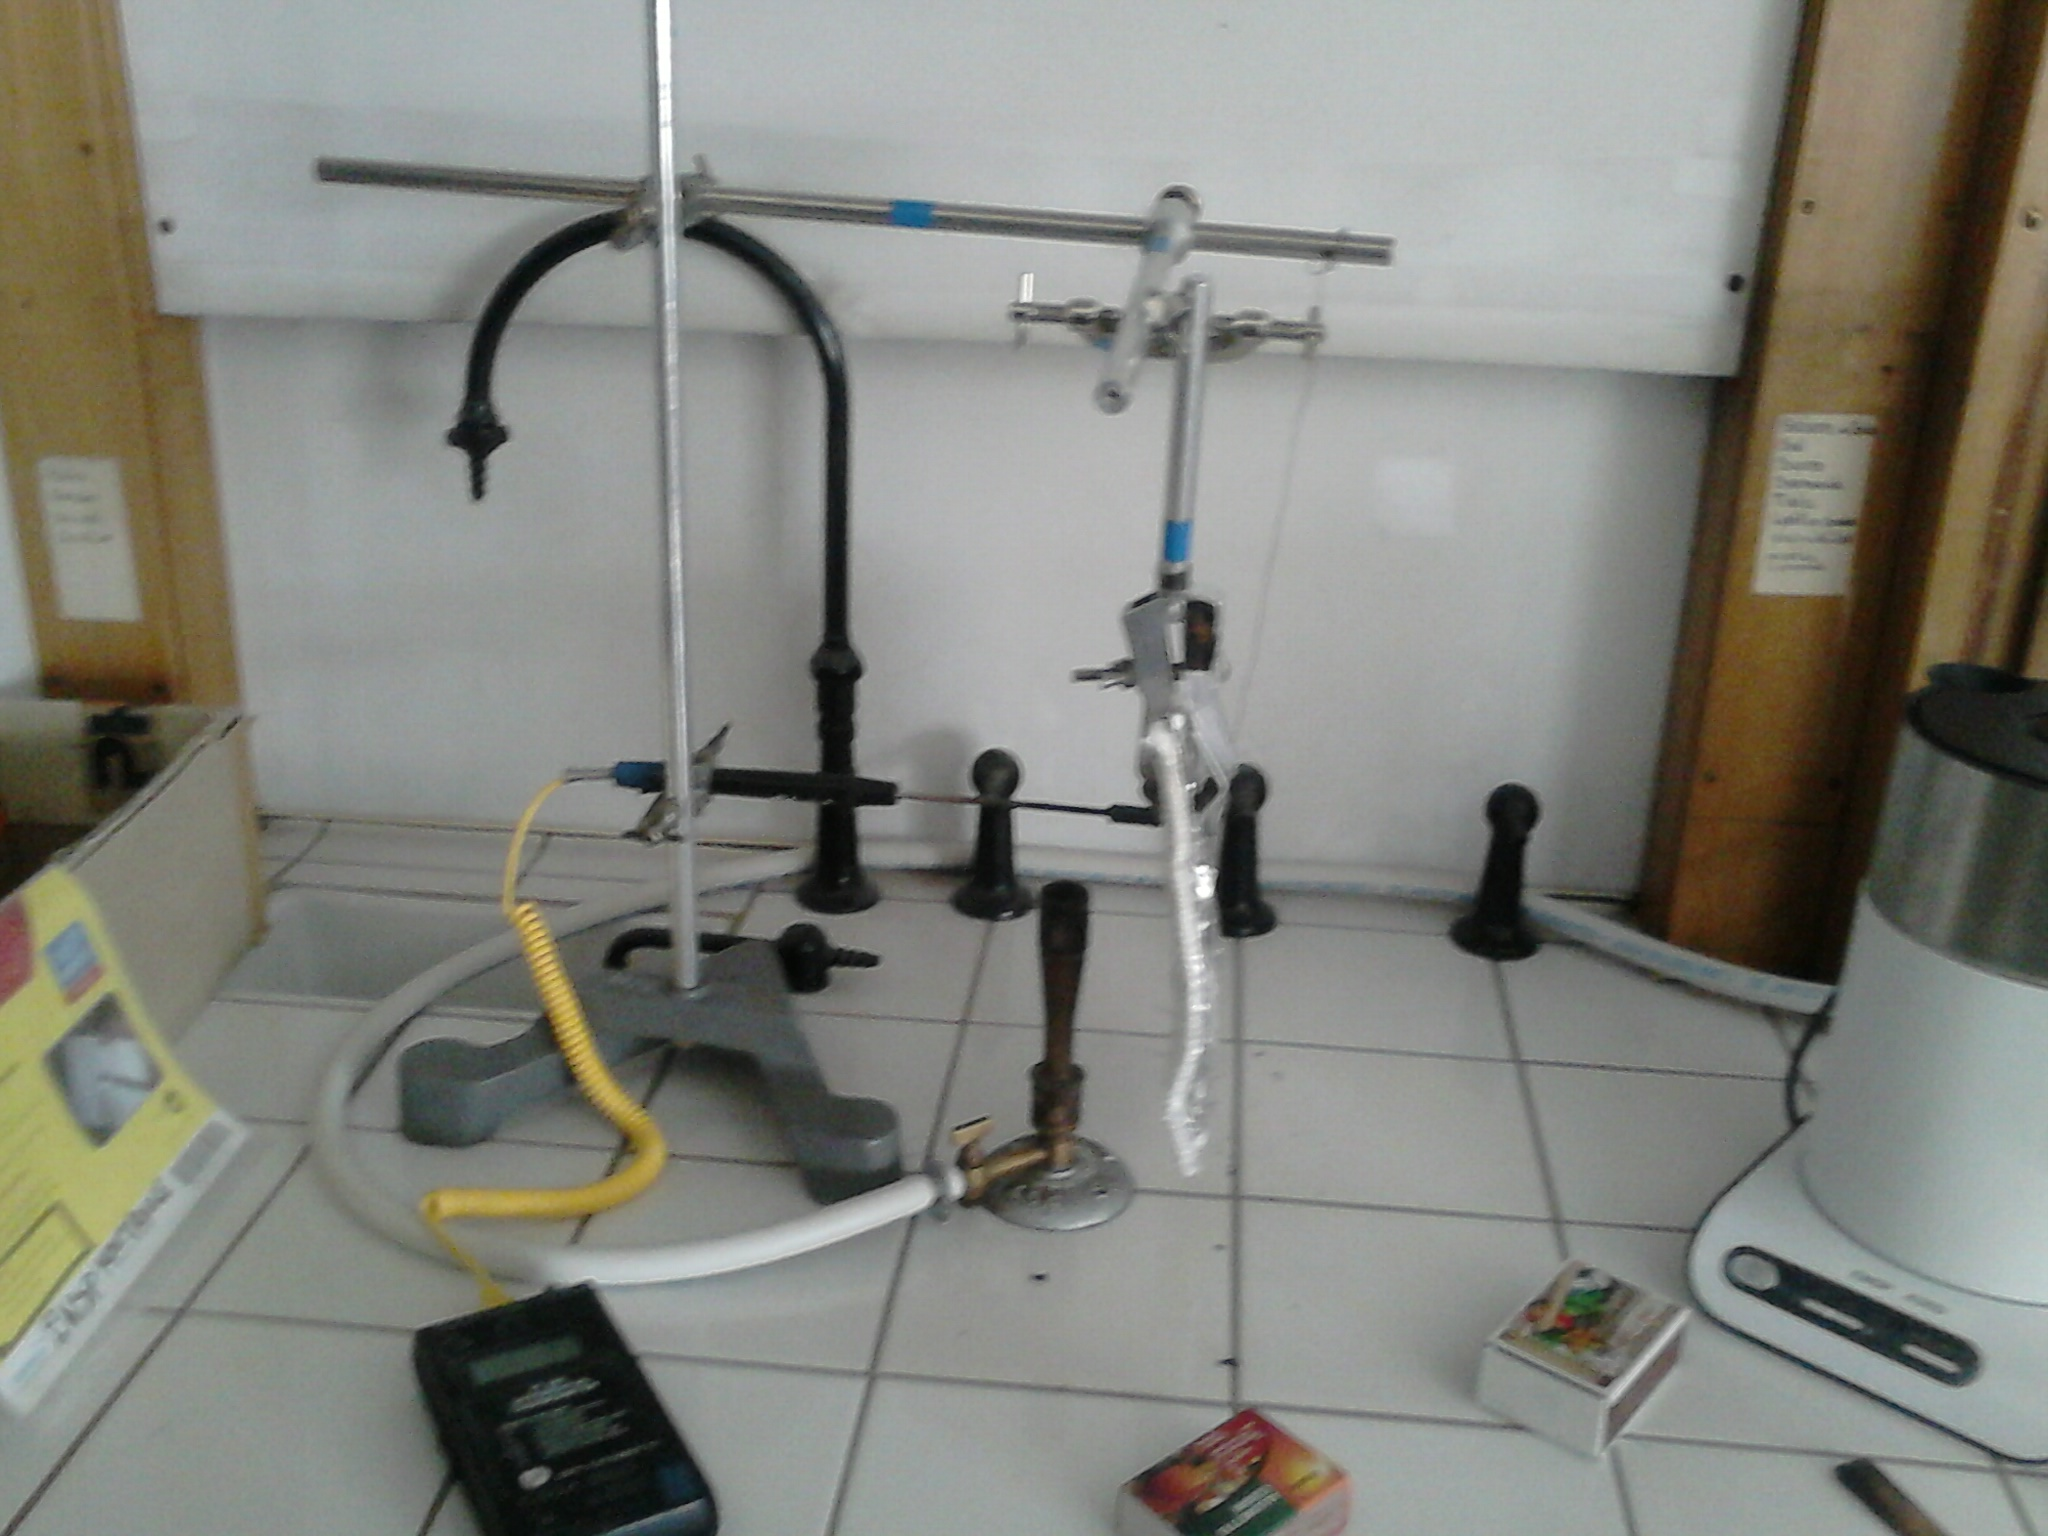
\includegraphics[width=5cm]{images-exp/transition_ferro_para.jpg}}
	\caption{Transition ferromagnétique-paramagnétique : Photo du dispositif}
\end{figure}

Réaliser cette expérience en utilisant le matériel prévu à cet effet : on chauffe avec un bec Mecker (température de flamme plus élevée que celle d'un bec Bunsen) une tige en fer percée dans laquelle on peut glisser un thermocouple chromel-alumel qui permet de mesurer la température. Un aimant, attaché à une ficelle et protégé par un écran anticalorique, est maintenu en position oblique par la tige au-dessous de $T_C$. Quand la tige atteint $T_C$, l'aimant reprend une position verticale. 

\underline{Ccl} : universalité du comportement

\og{}Bonus\fg{} : lévitation d'un semi-conducteur à basse température au-dessus d'un aimant en néodyme

\begin{figure}
	\centerline{\includegraphics[width=5cm]{images-exp/aimant_lévitation.jpg}}
	\caption{Transition vers état supraconducteur à basse température : Photo du dispositif}
\end{figure}

\section{Instruments d'optique.}
\underline{Références :}
\begin{itemize}
	\item Sextant 
	\item	Houard
\end{itemize}
\subsection{Lunette}
A construire et caractériser.

Comme le microscope, la lunette astronomique est formée de deux lentilles convergentes (une variante existe avec une lentille convergente et une divergente). Cependant, la lunette est conçue pour observer des objets à l'infini. On souhaite également une image sortante à l'infini pour que l'oeil n'ait pas besoin d'accomoder. C'est ce qu'on appelle un système afocal.

\textit{Schéma :}

Le schéma de principe d'une lunette est donné ci-dessous. L'objet sera l'image à l'infini d'un quadrillage, renvoyé à l'infini par une lentille convergente ($L_1$) de focale $20 cm$. La lunette astronomique est représentée par une lentille de grande focale ($L_2$) appelée objectif, et une lentille de petite focale ($L_3$) appelée oculaire, le foyer image de la première est confondu avec le foyer objet de la seconde. On modélise l’œil par une lentille convergente ($L_4$) de $20 cm$ également, munie d'un écran dans son plan focal image (œil sans accommodation). Réaliser le montage ci-dessous sur banc d'optique.

\begin{figure}
	\centerline{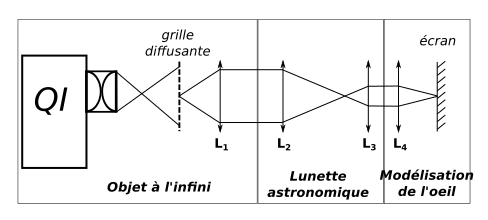
\includegraphics[width=5cm]{images-exp/Telescope.png}}
	\caption{Schéma de la lunette}
\end{figure}
\textit{Grossissement :}

L'objet AB étant à l'infini, le grandissement n'est pas une grandeur pertinente. Comme pour le microscope, on définit le grossissement $G=\frac{\theta'}{\theta}$, rapport des angles sous lesquels sont vus l'objet avec et sans lunette. Démontrer que
$G=\frac{\theta'}{\theta}\approx-\frac{f'_\textrm{ob}}{f'_\textrm{oc}}$

dans l'approximation des petits angles. Le signe moins témoigne du fait que l'image obtenue est renversée. Il faut donc choisir un objectif de grande focale (ici on prendra $f'_{ob}=50 cm$) et un oculaire de petite focale ($f'_{oc}=10$ ou $20 cm$). Noter que c'est l'inverse du microscope où on choisit un objectif de courte focale ! Mesurer expérimentalement le grossissement, et vérifier la formule ci-dessus.

\textit{Cercle oculaire :}

Le cercle oculaire est le lieu de convergence de tous les rayons passant à travers l'objectif. Il est habituellement situé derrière l'oculaire. Plus clairement, c'est l'endroit situé derrière l'oculaire où les rayons lumineux sont les plus concentrés. Le repérer. C'est à cet endroit qu'il convient de placer l’œil (ici la focale de $20 cm$) afin d'avoir le maximum de champ. La taille du cercle oculaire dépend-elle du grossissement de la lunette ? Quelle est la taille optimale du cercle oculaire ?


\subsection{Appareil photo, loi en $1/N^2$}

Vérifier la loi avec une photodiode en régime linéaire (branchée en inverse), pour n petit (gde ouverture) limitation par d'autres diaphragmes.

Nous commençons l'étude des instruments d'optiques par celle d'un objectif d'appareil photographique. Le but est de réaliser sur une pellicule fixe l'image d'un objet distant de quelques décimètres à l'infini [1]. On le modélise par une lentille convergente de distance focale f' [2].

Regarder l'objectif dont on dispose : on distingue une première bague de rotation permettant de modifier le tirage (distance entre la pellicule et l'objectif) pour que l'objet observé soit net. Les nombres allant de l'infini à 1.5 m aident à la mise au point en indiquant une distance approximative de netteté sur la pellicule (ici non présente, l'intérêt est donc limité). Plus proche du corps de l'objet se trouve une autre bague affichant des nombres entre 22 et 2,8 ; il s'agit de l'échelle des nombres d'ouverture permettant, grâce au contrôle de la taille d'un diaphragme, d'adapter le compromis entre luminosité et profondeur de champ : c'est l'objet de cette étude.

\textit{Nombre d'ouverture et profondeur de champ :}

En toute rigueur, un objet est net seulement s'il est dans le plan conjugué à celui de la pellicule. Cependant, l'expérience commune montre qu'il existe une certaine plage de tolérance, appelée profondeur de champ, sur laquelle une translation de l'objet laisse son image nette. Le passage à une image floue étant progressif, on recourt à un critère objectif pour définir cette profondeur de champ : on compare par exemple la taille de l'image d'un point sur la pellicule (le "cercle de confusion") à celle d'un pixel, ou à celle d'un grain en photographie argentique. Le schéma suivant illustre cette définition empirique  :
\begin{figure}
	\centerline{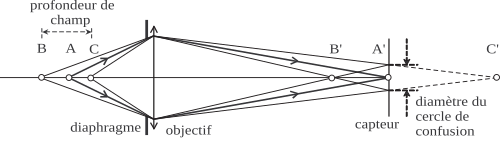
\includegraphics[width=5cm]{images-exp/InstrumentsProfChamp1.png}}
	\caption{Profondeur de champ et cercle de confusion}
\end{figure}

On remarque notamment sur cette figure que l'introduction proche de l'objectif d'un diaphragme, dont le diamètre sera noté D par la suite, augmente ainsi la profondeur de champ. Le nombre N= f'/D est appelé nombre d'ouverture : c'est celui affiché sur l'objectif[3]. Dans le cas particulier d'une mise au point à l'infini (photographie de paysage), on peut montrer que la profondeur de champ est proportionnelle à N .

Manipulation (cf. Sextant) : on propose ici une expérience qualitative montrant l'augmentation de la profondeur de champ avec le nombre d'ouverture. Éclairer une grille diffusante avec une lampe quartz-iode et faire l'image avec l'objectif d'appareil photo de cet objet sur un écran situé à environ un mètre (pour minimiser les aberrations géométriques décrites dans la suite de ce TP, orienter l'objectif dans le sens inverse au cas usuel, l'objet étant ici plus proche de l'objectif que l'image). Incliner maintenant la grille comme représenté sur la figure ci-dessous et observer l'influence du nombre d'ouverture sur l'image (en particulier le nombre de carreaux apparaissant nets).
\begin{figure}
	\centerline{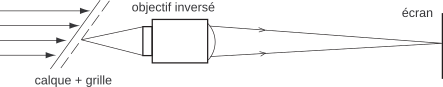
\includegraphics[width=5cm]{images-exp/InstrumentsProfChamp2.png}}
	\caption{Mesure de la profondeur de champ}
\end{figure}

Il est possible de rendre cette manipulation quantitative, en mesurant la profondeur de champ en fonction de l'ouverture de l'objectif (voir Sextant).

\textit{Nombre d'ouverture et éclairement :}

On pourrait penser qu'il faut toujours choisir le nombre d'ouverture le plus élevé disponible afin d'optimiser la profondeur de champ. Cependant, un grand nombre d'ouverture diminue fortement l'intensité lumineuse reçue sur la pellicule (inversement proportionnelle à $N^2$ ) et oblige à utiliser un temps de pose long entraînant des risques de bougé : il faut donc établir au cas par cas le bon compromis entre profondeur de champ et durée d'exposition.

Manipulation (inspirée du Sextant) : il est possible de montrer quantitativement la dépendance en $N^{-2}$ de l'intensité reçue sur la pellicule. Pour cela, remplacer la grille diffusante par un calque non incliné (ou tout du moins vérifier que le faisceau incident est homogène sur la surface de l'objectif), et accoler à l'objectif photographique, du côté opposé à celui de l'objet, une lentille de courte distance focale (10 centimètres). Positionner le capteur (luxmètre ou photodiode) de manière à capter tous les rayons issus de l'objectif, faire le zéro de manière appropriée pour s'affranchir de toute lumière diffusée et tracer l'intensité lumineuse en fonction de $N^{-2}$ en prenant en compte les incertitudes, puis vérifier la loi proposée. 

\subsection{Objectif de microscope}
Caractériser, bien se placer dans les conditions de fonctionnement.

\begin{figure}
	\centerline{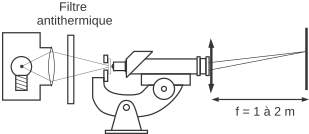
\includegraphics[width=5cm]{images-exp/InstrumentsMicroscope.png}}
	\caption{Etude du microscope}
\end{figure}
Le microscope a pour but de réaliser à partir d'un objet proche une image agrandie à l'infini (pour que l’œil n’accommode pas) dont les détails sont mieux perceptibles. Il est constitué d'un tube reliant deux cylindres, nommés objectif et oculaire et modélisés par des lentilles convergentes : le premier fait de l'objet une image intermédiaire, agrandie, située dans le plan focal objet du second (utilisé comme une loupe : il renvoie l'image agrandie à l'infini). Chacun de ces constituants participe à l'agrandissement de l'image, mais du fait de leur fonction différente, on est amené à quantifier cet effet via deux grandeurs distinctes :

\begin{itemize}
	\item pour l'objectif, le chiffre gravé sur le cylindre (x4, x10, x60) est son grandissement $\gamma_{ob}$ , i.e. le rapport entre deux tailles : celle de l'image intermédiaire et celle de l'objet ( $\gamma_{ob} <0$ car l'image est renversée)

	\item pour l'oculaire, il s'agit en revanche de son grossissement commercial $G_{c,oc}$ (x6, x10, x15), à savoir le rapport entre deux angles : celui sous lequel est vu l'objet après l'oculaire et celui sous lequel il est vu sans oculaire à une distance de $25 cm$ (le punctum proximum)

	\item pour le microscope entier, on utilise aussi le grossissement commercial et on peut alors montrer que $G_{c,mic}=G_{c,oc} \vert \gamma_{ob} \vert$
\end{itemize}

\textit{Mesure du grossissement commercial :}

Manipulation (cf. Sextant) : Disposer le microscope horizontalement comme indiqué sur la figure et le poser sur un support élévateur. Placer une mire graduée en dixièmes de millimètre dans la platine porte-objet et choisir par exemple $\gamma_{ob}=4$ et $G_{c,oc} = 10$. Éclairer l'objet grâce à une lampe quartz-iode avec un condenseur de courte focale faisant converger le faisceau sur l'objet. Il est indispensable de prendre l'habitude de placer entre le condenseur et l'objet un filtre antithermique pour éviter une destruction rapide de l'objet. Placer juste après l'oculaire une lentille de grande focale (1 à 2 m) et un écran dans le plan focal. Régler le microscope pour que l'image de la mire soit nette sur l'écran, mesurer l'angle sous lequel on voit une graduation de la mire à la sortie du microscope, en déduire le grossissement commercial du microscope et vérifier la relation $G_{c,mic}=G_{c,oc} \vert \gamma_{ob} \vert$ .

\textit{Autres manipulations possibles :}

La profondeur de champ est définie de manière différente pour l'objectif d'appareil photo et le microscope (l’œil accommodant au maximum pour toujours avoir une image nette sur la rétine), sa valeur variant typiquement entre le micron et la centaine de microns pour ce dernier appareil : il est cependant délicat d'en faire une mesure quantitative. D'autres expériences concernant le microscope sont néanmoins réalisables, on se référera par exemple au Sextant ou à Optique (S. Houard). 

\section{Interférences lumineuses.}
\underline{Références :}
\begin{itemize}
	\item Sextant
	\item  Bottineau
\end{itemize}
\subsection{Fentes d'Young}
barette CCD
division du front d'onde

    Comme le montre la figure 1, on propose l'expérience sous sa forme classique, sans utiliser de lentille après la fente source. Il ne s'agit pas d'une expérience de diffraction de Fraunhofer.
\begin{figure}
	\centerline{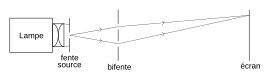
\includegraphics[width=5cm]{images-exp/Fentes_Young2.png}}
	\caption{Fentes d'Young : schéma du dispositif}
\end{figure}

    \textit{Choix de la source :}
    Lampe Quartz-Iode[1]. Pourquoi le laser ne permet-il pas de faire l'expérience (importante) de cohérence spatiale?

    \textit{Choix du condenseur :}
    Comparer la zone éclairée sur l'écran dans le cas d'un condenseur très convergent puis très peu convergent. Si l'on veut que la luminosité sur l'écran soit élevée lequel a-t-on intérêt à choisir[2]?

    \textit{Choix de la fente source :}
    Choisir une fente réglable étalonnée (pour l'expérience de cohérence spatiale), s'entraîner à la régler et à lire sa largeur. Le faisceau doit couvrir toute sa surface, et en pratique, afin de réduire la lumière parasite, il est conseillé de placer la fente contre le condenseur. Régler la fente à sa largeur maximum. Constater que l'on voit sur l'écran l'image indésirable du filament. En déplaçant un petit écran mobile remarquer que cette image est très délocalisée : il s'agit d'un effet de profondeur de champ, plus on diaphragme plus le champ en profondeur est grand (cf. poly Instruments d'optique). Remarquer ensuite qu'en réduisant beaucoup la largeur de la fente, l'image du filament sur l'écran devient floue, donc non gênante, à cause de la diffraction. Les expériences qui suivent imposent de travailler avec une fente fine, donc on sera toujours à peu près dans ce cas[3].

    \textit{Choix de la bifente :}
    Choisir une bifente photographique dont la distance a entre les deux traits est comprise entre $0,2$ et $0,3 mm$. Il y a aussi une bifente gravée sur plaque inox mince mais celle-ci n'est pas conseillée ici car $a = 0,6 mm$ est un peu trop grand. Placer la bifente à $10-30 cm$ de la fente source (à ajuster, plus cette distance est grande et plus on peut élargir la fente source, mais il ne faut pas trop réduire l'interfrange sur l'écran. Expliquer en termes d'angle de cohérence).

    Observer les franges sur un écran à environ 2 m. Élargir progressivement la fente source en faisant un compromis entre luminosité et contraste. Bien régler le parallélisme fente-bifente. Pour rendre l'expérience visible de loin, interposer un petit écran mat fortement incliné vers l'auditoire. Expliquer les irisations.

    Vérifier la non localisation des franges en déplaçant l'écran. 

    Placer des filtres interférentiels (les filtres colorés ordinaires n'ont pas de longueur d'onde affichée, ils peuvent cependant servir à faire une première présentation sans mesure) et vérifier quantitativement la loi donnant l'interfrange. Le phénomène est très peu lumineux. Pour le rendre plus visible pour l'auditoire on peut utiliser une Webcam avec son objectif dirigé vers l'écran mat et observation sur l'écran de l'ordinateur étalonné avec une règle, ou placer une barrette CCD. À tester mais ces techniques risquent de vous prendre pas mal de temps à chaque fois. Avec ces appareils le contraste peut être meilleur si on ajoute un filtre antithermique.

    \textit{Expérience de cohérence spatiale :} Étudier l'influence de la largeur de la fente source. En élargissant la fente source on observe le brouillage puis la réapparition des franges avec inversion du contraste[4]. Il faut faire une exploitation quantitative du premier brouillage, mais on ne peut pas en attendre une grande précision, on peut donc opérer rapidement en utilisant un filtre coloré orange (environ 600 nm[5]) à la place d'un filtre interférentiel. Dans ce cas l'expérience est beaucoup plus lumineuse. Elle est visible de loin en inclinant l'écran. Sinon webcam ou barrette CCD.

\subsection{Lame de savon}
Division d'amplitude
semi-qualitative

Pour augmenter la tenue des lames on peut interposer un filtre anti-thermique.

\begin{figure}
	\centerline{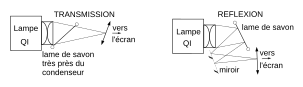
\includegraphics[width=5cm]{images-exp/Film_Savon.png}}
	\caption{Lame de Savon : schéma du dispositif}
\end{figure}
Le montage par transmission est facile à mettre en œuvre mais donne un très faible contraste des franges (expliquer). L'expérience peut cependant être réalisée en inclinant fortement la lame autour d'un axe vertical ce qui augmente le coefficient de réflexion. Pour accroître la zone de netteté, incliner un peu la lentille vers la lame comme indiqué[17] sur la figure 2.

Pour réaliser le montage par réflexion, plus délicat à mettre en œuvre, il est préférable d'opérer en incidence proche de la normale, car à partir de l'incidence de Brewster le comportement change (notamment en phase).

\begin{itemize}
	\item    Pourquoi ne voit-on pas de franges quand la lame est épaisse?
	\item    Ajouter un filtre interférentiel. Que se passe-t-il?
	\item    Pourquoi avant l'éclatement la partie la plus mince apparaît-elle noire dans le montage par réflexion ?
\end{itemize}

\subsection{Michelson, longueur de cohérence de la lampe à vapeur de sodium}
Division d'amplitude

Prendre une lampe à vapeur de sodium[9] avec un condenseur de $70 mm$ et travailler en anneaux. Charioter. Observer que pour certaines différences de marche le contraste s'annule (anti-coïncidence). Mesurer le chariotage $\Delta e$ correspondant au passage d'une anti-coïncidence à la suivante (s'entraîner à lire correctement les indications de chariotage). En déduire $\Delta \lambda$ par la formule:
\[\Delta \lambda = \frac{\lambda ^2}{2\Delta e}\]

Que faire pour améliorer la précision ?

En fait cette manipulation est un exemple élémentaire de spectroscopie par transformée de Fourier étudiée dans le paragraphe suivant. 

\section{Diffraction des ondes lumineuses.}
\subsection{Fente}
Diffraction par une fente en lumière laser

Envoyer directement le faisceau laser sur une fente étalonnée de largeur variable[3]. Si les bords de la fente sont en biseau, il faut que celui-ci soit du côté émergent des rayons (figure 4).

Observer la figure de diffraction. Comment est-elle modifiée quand on change la largeur de la fente diffractante ?
Exploitation quantitative

Il s'agit de mesurer la distance entre les lobes de la figure de diffraction ainsi que les intensités des maxima successifs, puis de confronter ces mesures à la théorie.

\textit{Méthode rapide}

    Fermer nettement la fente réglable étalonnée de façon à ce que le lobe central occupe plusieurs cm. Mesurer l'écartement entre les lobes avec une règle. Mesurer les intensités lumineuses contenues dans les lobes principaux avec une photodiode auto-alimentée. Pour cette mesure, il faut que la largeur du détecteur soit petite devant celle d'un lobe[4], sinon diaphragmer le capteur avec de l'adhésif noir.

\textit{Méthode longue}

    On peut également enregistrer la figure de diffraction à l'aide d'une caméra pour en faire un ajustement par la loi en sinc2. Le mieux est d'utiliser une barrette CCD Mightex, qui a un grand nombre de niveaux de gris (16 bits) (l'utilisation d'une webcam utilisée comme CCD en ôtant l'objectif est déconseillé). Bien faire attention au parallélisme entre la barrette CCD et la figure de diffraction.
    Les signaux obtenus avec un laser sont souvent bruités à cause du speckle et facilement déformés. À ce titre on aura parfois moins de problèmes en utilisant un faisceau laser élargi ou une source conventionnelle filtrée (utiliser en priorité un laser seul, et ne changer de source lumineuse que si c'est vraiment nécessaire).
    Une autre difficulté est liée à la grande sensibilité du capteur Mightex. En particulier, il est difficile d'observer simultanément le pic principal et les lobes secondaires du sinus cardinal sans que le premier soit saturé ou que les seconds soient noyés dans le bruit. Pour observer les lobes secondaires, on peut placer volontairement le pic principal en dehors de la barrette CCD. Pour observer le pic principal, on aura souvent intérêt à réduire le temps d'exposition et/ou à réduire l'intensité lumineuse en utilisant des filtres de densité (placé directement en sortie du laser) ou des polariseurs croisés[5].

    L'expérience montre que la méthode longue fonctionne bien avec la caméra CCD linéaire Mightex (voir image de la notice de cette caméra). Mesurer les tailles du lobe principal et des lobes secondaires et vérifier qu'elles correspondent aux valeurs attendues. Idéalement, on fera un ajustement de l'intensité lumineuse par la loi en sinc2 (ajouter une constante dans l'ajustement si l'on ne soustrait pas le niveau de bruit). Attention, pour sauvegarder le profil au format txt, il faut indiquer un nom de répertoire autre que C:, sinon le logiciel plante.
\subsection{Poudre de lycopode}
Grains répartis aux hasard=> les intensités lumineuses s'additionnent, pas d'interférences. Détermination du rayon des spores avec le rayon de la tache d'Airy

On peut aussi observer la diffraction par des spores de lycopode, alias pied-de-loup. Déposer la poudre sur une plaque de verre embuée, au-dessus d'une feuille de papier, et récupérer le surplus (une plaque déjà préparée est aussi disponible dans la collection). Comparer le résultat en éclairage direct et élargi. Constater que la figure de diffraction est la même que celle obtenue avec un object diffractant en forme de trou[7], sauf au centre de la figure (pourquoi ?). On illustre ainsi le théorème de Babinet, voir section IV.1.

La figure ici obtenue est la figure de diffraction par de nombreux objets identiques répartis aléatoirement. Pourquoi peut-on déduire de cette expérience que les spores ont des diamètres voisins ? Mesurer la diamètre moyen des spores.

On peut comparer la taille trouvée avec une mesure obtenue par observation directe des spores, au moyen de l'ensemble microscope + caméra vidéo + moniteur (faire la calibration en observant la mire graduée au moyen du même dispositif), ou plus simplement du microscope seul.

On observe une tache d'Airy, dont on mesurera le rayon du 1er anneau. Vérifier qu'il correspond à un angle de diffraction $\theta\approx 1,22 \lambda/d$, où d est le diamètre du trou et $\lambda$ la longueur d'onde du laser.


\subsection{Réseau}
Goniomètre, montrer le figure théorique d'interférence
Appli mesure raies d'une lampe spectrale (hydrogène). Attention à l'intensité des lampes pour ne pas endommager les yeux.

Observer maintenant la figure de diffraction par un réseau "classique". On l'a déjà rencontré dans le TP Propriétés des instruments d'optique. Dans le cadre du montage Diffraction des ondes lumineuses, on pourra

\begin{itemize}
	\item    examiner l'influence du nombre de traits par unité de longueur sur la distance entre les ordres,
	\item    examiner l'influence du nombre de fentes éclairées sur le pouvoir de résolution (par exemple en utilisant une fente réglable dont on pourra facilement changer la largeur),
	\item    déterminer si les réseaux étudiés sont "blazés"[9], i.e. si le maximum d'intensité est placé dans un ordre de diffraction non nul, typiquement 1 ou -1 (il peut alors être utile de passer en lumière blanche afin d'utiliser l'absence de dispersion dans l'ordre 0 de diffraction et ainsi le repérer facilement).
\end{itemize}

\textit{Description :}

Un goniomètre est un appareil permettant de mesurer de manière précise des angles. On va s’en servir ici pour déterminer les longueurs d’onde des raies d’émission d'une lampe spectrale. Le but du réglage consiste à observer à travers la lunette afocale (observation a l’infini) les rayons émergents de la fente source à l’infini (donc parallèles) après déviation par un élément dispersif (réseau ou prisme). Il faut aussi aligner les axes de la lunette et du collimateur, qui doivent être perpendiculaires aux éléments dispersifs. Les angles se lisent à l’aide d’un système de vernier via le deuxième oculaire placé sous la lunette.
\begin{figure}
	\centerline{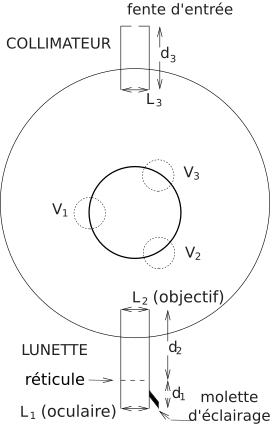
\includegraphics[width=5cm]{images-exp/FigureGonioDessus.png}}
	\caption{Goniomètre : schéma de l'appareil}
\end{figure}

\textit{Réglage optique :}

Commençons par le réglage de la lunette autocollimatrice d’observation. Régler d’abord la distance $d_1$ (tirage de l’oculaire) de manière à voir net le réticule (croix) sans accommoder (i.e. en relâchant complètement le cristallin de l’œil). Ce réglage peut dépendre de la vision de chaque utilisateur. Basculer vers l’avant la manette sur le côté de l’oculaire : on éclaire ainsi le réticule avec une lampe par l’intermédiaire d’une lame semi-réfléchissante. Le réticule peut donc alors servir d’objet pour un réglage par autocollimation. Placer un miroir devant l’objectif de la lunette, et régler la distance $d_2$ (tirage de l’objectif) de manière à voir nets simultanément le réticule et son image réfléchie par le miroir. Rebasculer la manette et enlever le miroir. La lunette est alors réglée pour une observation à l’infini : les foyers de $L_1$ et $L_2$ sont confondus, et le réticule est dans leur plan. Réglons maintenant le collimateur, en l’alignant avec la lunette d’observation. Ajuster la distance $d_3$ de manière à voir net les bords de la fente d’éclairage dans le même plan que le réticule. La fente est alors dans le plan focal objet de la lentille $L_3$ , qui produit donc un faisceau de rayons parallèles.

\textit{Réglage de l'horizontalité de la lunette :}

On va maintenant régler les alignements des différents éléments du goniomètre. L’axe du collimateur est par construction perpendiculaire à l’axe de rotation de la partie inférieure du plateau central ; par contre l’horizontalité de l’axe de la lunette est réglable par une vis (appelée $V_0$ dans la suite), tandis que la partie supérieure du plateau central est orientable librement par rapport à la partie inférieure à l’aide des vis $V_1$, $V_2$ et $V_3$ :

Régler grossièrement les trois vis du plateau autour de leur mi-course, de manière a avoir le plateau à peu près horizontal. Ajuster de même $V_0$ pour rendre, à vue d’œil, la lunette horizontale. On va régler précisément $V_0$ de manière à rendre l’axe de la lunette perpendiculaire à l’axe de rotation de la partie inférieure du plateau (et ainsi colinéaire au collimateur). Pour cela poser la lame à faces parallèles sur le plateau, avec les faces parallèles à l’axe défini par deux des trois vis du plateau.


Éclairer le réticule à l’aide de la manette sur le côté. On va faire un réglage par auto-collimation en utilisant la réflexion sur la face avant de la lame. Aligner la lunette perpendiculairement à la lame, de manière à voir le réticule et son image ; amener à coïncidence leurs bras horizontaux, en faisant la moitié du chemin avec $V_0$ et l’autre moitié avec $V_1$ . Faire pivoter le plateau de 180 degrés. Recommencer le réglage de $V_0$ et $V_1$, faire pivoter de nouveau le plateau, ainsi de suite jusqu’à ce que la coïncidence persiste sur les deux faces de la lame. L’axe de la lunette est alors perpendiculaire à l’axe de rotation central, quelque soit l’angle de contact entre la lame et le plateau :

Il ne faut plus toucher à $V_0$ à partir de maintenant.

\textit{Utilisation avec un réseau}

Placer le réseau au centre de la plate-forme centrale du goniomètre, parallèle à l’axe défini par deux des trois vis du plateau (cf. figure précédente pour la lame). Il faut régler les trois vis du plateau pour que le plan du réseau soit perpendiculaire au faisceau lumineux, et pour que ses traits soient parallèles à l’axe de rotation du goniomètre. Le premier réglage se fait en jouant sur $V_1$ : avec le réticule éclairé, ajuster cette vis pour que les bras horizontaux du réticule et de son image par réflexion sur une des faces du réseau coïncident. Avant la suite du réglage, vérifier que la fente d'éclairage est bien verticale. Supprimer l’éclairage du réticule ; approcher une lampe spectrale de la fente d’éclairage, en masquant les lumières parasites. Vérifiez que vous voyez les différentes raies dans la lunette d’observation. Régler la largeur de la fente d’illumination la plus fine possible de manière à avoir une plus grande précision dans la lecture des angles, mais assez large pour que l’intensité lumineuse soit suffisante. Régler les vis $V_2$ et $V_3$ de manière à avoir des raies verticales ; on peut aussi masquer la fente d’illumination de manière à ne garder qu’une petite portion verticale des raies de diffraction, et vérifier qu’elles sont toutes alignées horizontalement.

\textit{Mesures :}

Pour une plus grande précision dans la détermination de la longueur d'onde d'une raie par un réseau à transmission, il faut utiliser la méthode du minimum de déviation[1]. Celle-ci permet d'éviter une mesure absolue des angles d'incidence sur le réseau. On se trouve alors dans la configuration schématisée ci-dessous :
MinimumDeviationReseau.svg

On a alors $2a \sin(\theta_{0})=-p\lambda$, à savoir démontrer. Mesurer la déviation $ D=2\theta_{0}$, en déduire la longueur d’onde correspondante. Pour une meilleure précision, on peut choisir un ordre de diffraction élevé (voire effectuer un ajustement à partir de tous les ordres visibles...).

Un calcul rapide peut vous convaincre qu'il n'existe pas de minimum de déviation pour un réseau en réflexion.

%\subsection{Filtrage spatial et strioscopie}
\section{Spectrométrie optique.}

\underline{Références :}
\begin{itemize}
	\item Sextant
\end{itemize}

\subsection{Etalonage d'un spectromètre (réseau)}

Avec gonio (voir au-dessus), lampe spectrale (hydrogène)

Idem en supposant les valeurs des longueurs d'onde connues.

\subsection{Mesure par spectromètre USB}
Interférence de polarisation,spectre cannelé (1 nm précision)

On étudie, par exemple, une lame de quartz taillée parallèlement à l'axe optique.

    Réaliser le spectre d'une lampe quartz-iode à l'aide d'une fente F et d'un prisme à vision directe (on fera l'image de la fente sur l'écran à l'aide de la lentille, et on ajoutera ensuite le prisme à vision directe). Ajouter deux polariseurs croisés. Placer la lame Q entre P et A. Faire tourner Q dans son plan de manière à obtenir l'image la plus éclairée. Observer le spectre cannelé. On vérifiera que la rotation de Q modifie l'éclairement mais ne modifie ni le contraste ni la position des cannelures.[3] À quelles longueurs d'onde correspondent les cannelures ? Combien d'entre elles s'attend-on à voir ?

ATTENTION: ni la lentille ni le prisme ni la lame Q ne doivent diaphragmer le faisceau.

    Interposer successivement deux filtres étalonnés ayant une largeur à mi-hauteur d'environ 10 nm, pour repérer la position de deux cannelures. En admettant que la dispersion du quartz est négligeable sur le spectre visible, en déduire la valeur de $\Delta n = n_e - n_o$ , que l'on comparera à la valeur tabulée. Pour plus de précision, on peut aussi remplacer le prisme à vision directe par une fibre reliée à un spectromètre USB.

    Tourner l'analyseur de 90°. Expliquer qu'on observe le spectre complémentaire. L'expérience suivante permet de le mettre en évidence dans le cas d'une lame mince.
\subsection{Mesure par interférométrie avec le Michelson}
Cohérence spatiale/temporelle

L'interféromètre de Michelson met en évidence le phénomène de cohérence temporelle : à cause de la largeur spectrale de la source, les interférences ne sont présentes que sur un intervalle spatial nommé longueur de cohérence, variant pour les sources classiques de quelques microns (lampe Quartz-Iode) à quelques centimètres (lampe spectrale). On se propose ici de montrer l'un des aspects importants du laser, à savoir sa longueur de cohérence, qui peut atteindre plusieurs centaines de mètres pour des lasers ordinaires, des secondes ou heures lumière pour les lasers les plus stables.
InstrumentsCoherenceTemporelleMichelson.svg

Manipulation (cf. Sextant) : Grâce à cette facilité d'obtention d'interférences avec un laser, il est possible de réaliser un interféromètre de Michelson en agençant à la main les composants. Réaliser le schéma ci-dessus de la manière suivante :

    Placer le miroir $M_{1}$ près de la séparatrice et régler son orientation pour qu'une partie du spot revienne juste au dessus de la sortie du laser (ne pas le faire revenir directement dans le laser, car le couplage entre les faisceaux «aller» et «retour» dans le tube peut induire des franges parasites et des instabilités).
    Placer le miroir $M_{2}$ de façon à introduire une différence de marche de l'ordre de 1 m. Pour le réglage de l'orientation, procéder comme pour $M_{1}$.
    Placer la lentille de très faible distance focale à la sortie de la séparatrice. Observer sur l'écran les deux faisceaux étalés et retoucher l'orientation d'un des miroirs pour que ces deux faisceaux aient une région commune. Si vous n'observez pas de franges, cela peut être dû à une anticoïncidence entre les différents modes longitudinaux du laser, déplacer $M_{1}$ d'environ $10 cm$ et reprendre le réglage.

Le fait d'observer des franges (avec une visibilité acceptable) prouve que la longueur de cohérence est supérieure à la différence de marche des deux faisceaux : on mesure ainsi une borne inférieure pour la longueur de cohérence (déjà au dessus de celles des sources classiques). Ce montage permet avec un peu plus de travail de mettre en évidence le caractère multimode des lasers de la collection (i.e. ayant un spectre composé non pas d'une mais de plusieurs raies très fines), on se référera pour cela au Sextant. 

\section{Émission et absorption de la lumière.}
\underline{Références :}
\begin{itemize}
	\item Sextant
\end{itemize}

\subsection{Emission spontanée}

Spectre d'émission d'un atome (niveaux Rydberg) , hydrogène s'il y a la lampe.
Avec prisme (montrer spectre) et goniomètre (mesure précise)

cf plus haut
\subsection{Absorption d'un semi-conducteur, mesure de l'énergie du gap}
Avec l'illuminateur monochromateur, illuminer le conducteur, mesure sur photodiode, tracé intensité en fct $\lambda$, absorption

Retrouver la relation numérique liant la longueur d'onde en $\mu m$ à l'énergie en $eV$ d'un photon. Cette relation servira dans tout ce qui suit.
Absorption fondamentale d'un semiconducteur

Un cristal semiconducteur, transparent pour $hc/\lambda$ très petit devant le gap $E_g$, devient opaque lorsque $hc/\lambda$ dépasse $E_g$ : un photon a alors en effet une énergie suffisante pour exciter un électron de la bande de valence dans la bande de conduction.

On dispose ici de deux échantillons : GaAs, d'aspect "opaque", et GaP, "orange". Utiliser ces simples observations visuelles pour situer les gaps de ces semiconducteurs par rapport aux limites du visible, qui sont 1,6 eV (rouge) et 3,1 eV (bleu).
[1P] Détermination du gap de GaP

Une source de lumière blanche (illuminateur) est placée à l'entrée d'un monochromateur. L'échantillon de GaP est plaqué contre la fente de sortie. Placer un écran blanc une vingtaine de centimètres plus loin.
\begin{figure}
	\centerline{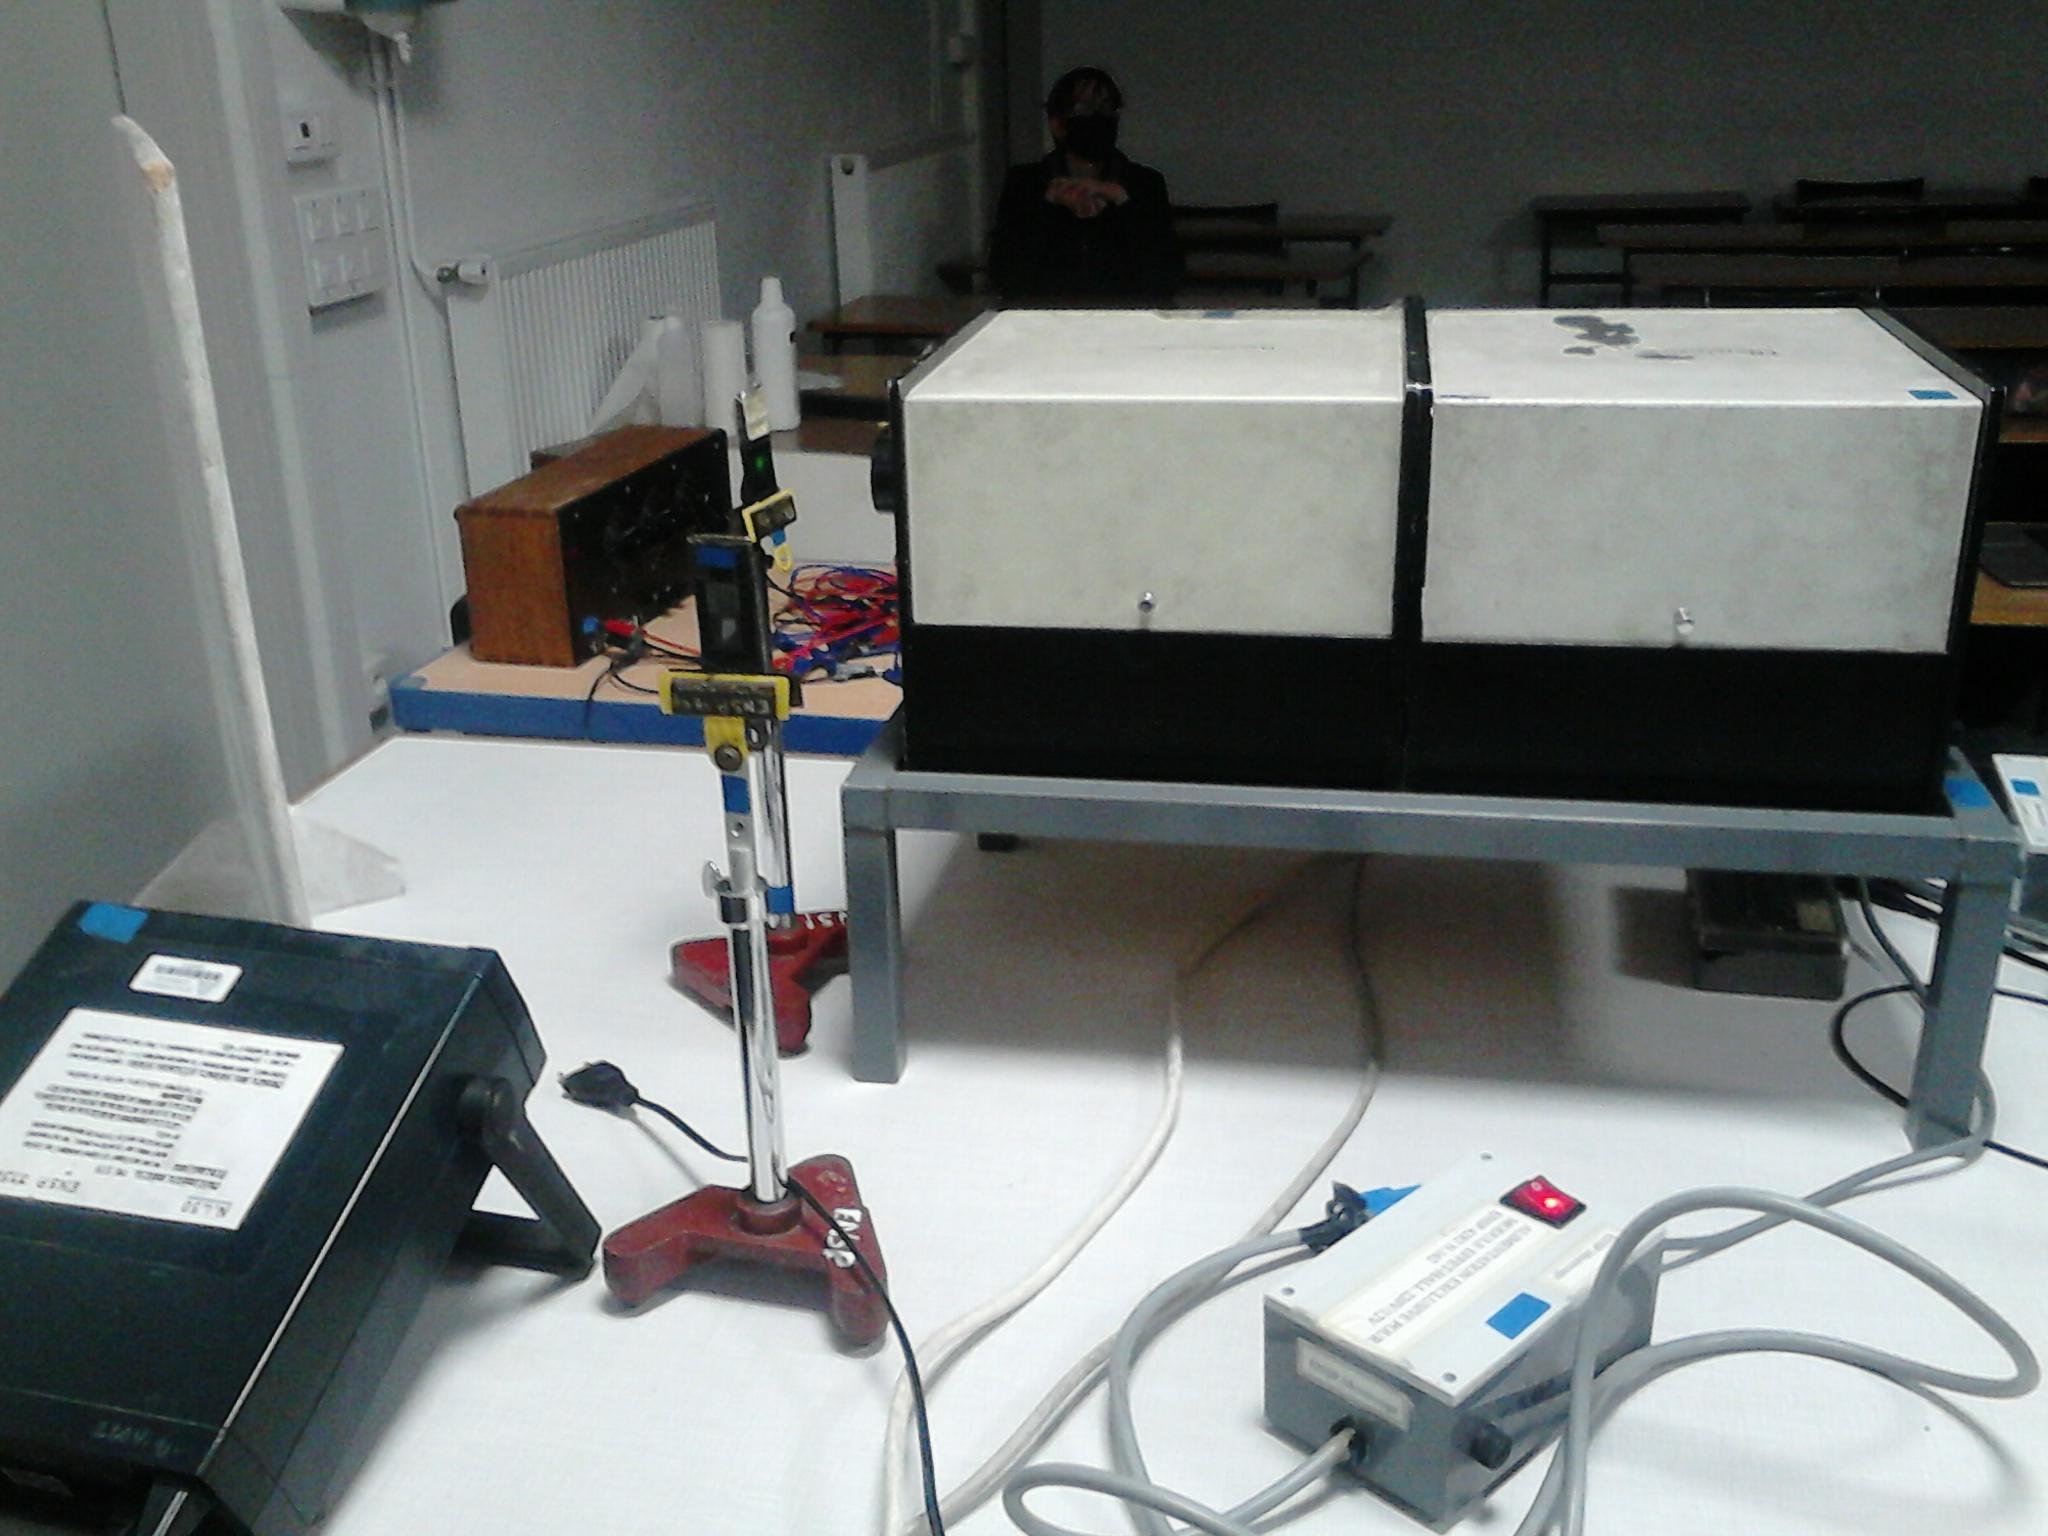
\includegraphics[width=5cm]{images-exp/gap_monochromateur.jpg}}
	\caption{Absorption d'un semi-conducteur, mesure de l'énergie du gap : Photo du matériel}
\end{figure}

Faire défiler à la main les longueurs d'onde. Observer que le rouge, le jaune, le vert sont transmis, puis que l'échantillon devient opaque aux longueurs d'onde plus courtes.

Déduire du seuil de l'absorption fondamentale ainsi mise en évidence une estimation du gap de GaP.

N.B. : On peut aussi envisager de faire cette expérience avec un des spectromètres USB, en enregistrant successivement un spectre de référence et un spectre de la lumière transmise à travers l'échantillon et en faisant le rapport des deux.
[2P] Détermination du gap de GaAs

Celui-ci se trouve dans le domaine du proche infrarouge. Il est donc nécessaire de modifier le montage précédent pour remplacer l'œil par un détecteur sensible dans l'infrarouge : la photodiode au silicium.

Placer l'échantillon de GaAs contre la fente de sortie, immédiatement suivi par une photodiode au silicium, polarisée en inverse. On prendra pour R une résistance de l'ordre de $100 k\Omega$.


L'enregistrement n'est pas indispensable. On peut se contenter d'observer "à la main" le signal transmis. Commencer les réglages avec des fentes de l'ordre du mm. Les réduire ensuite si le signal est suffisant. A partir de la courbe obtenue, déterminer la valeur de la largeur de bande interdite du semiconducteur. Le choix de la position du seuil sur la courbe de transmission est néanmoins délicat.
\subsection{Absorption et émission d'un colorant : fluorescence}
Mesure cuve rodamine, spectroscope USB et prisme

\underline{Définition fluorescence (wikipédia)}

La fluorescence est une émission lumineuse provoquée par l'excitation des électrons d'une molécule (ou atome), généralement par absorption d'un photon immédiatement suivie d'une émission spontanée. Fluorescence et phosphorescence sont deux formes différentes de luminescence qui diffèrent notamment par la durée de l'émission après excitation : la fluorescence cesse très rapidement tandis que la phosphorescence perdure plus longtemps. La fluorescence peut entre autres servir à caractériser un matériau.


\section{Photorécepteurs.}
\underline{Références :}
\begin{itemize}
	\item Sextant
	\item Kittle
\end{itemize}

\subsection{Photodiode}

Linéarité, caractéristique, sensibilité,sensibilité spectrale, temps de réponse
s'affranchir de la résistance en mesurant $u_D$ et en utilisant un transformateur d'isolement.
Utiliser une grande valeur de résistance pour voir l'effet du flux lumineux

La lumière crée des porteurs dans une jonction p-n et augmente le courant inverse dû aux porteurs minoritaires. Pour un fonctionnement en régime linéaire, une photodiode doit être utilisée avec une polarisation inverse externe (voir plus bas). Nous disposons de photodiodes au silicium (gap indirect à $1,14 eV$ correspondant à $1,1 \mu m$ ; modèles BPX 61 et BPW 34) dont le maximum de sensibilité est dans l'infrarouge proche ($ \sim 0,85 \mu m$).
[1P] Caractéristique courant -- tension

On l'obtient à l'oscilloscope grâce au montage de la Fig. 1 (la résistance sert à la fois à mesurer et à limiter le courant) :
Montage de la photodiode pour la caractéristique courant-tension

Régler le décalage et le niveau du GBF pour explorer la caractéristique. En l'absence d'éclairement on a la caractéristique usuelle d'une diode (le courant pour des tensions très négatives est alors appelé courant d'obscurité). Observer sa modification quand on augmente le flux lumineux~$\Phi$.
Caractéristique courant-tension de la photodiode

On passe d'une caractéristique à l'autre par un décalage vertical proportionnel au flux : $ I = k \Phi$ .

Note : idéalement il faudrait un oscilloscope différentiel pour avoir la tension aux bornes de la diode, sinon la résistance qui sert à mesurer le courant introduit une erreur sur cette tension. L'erreur est cependant sans importance dans la zone où les caractéristiques sont horizontales, l'effet étant dans ce cas un décalage horizontal.
[1P] Utilisation de la photodiode en détecteur de lumière linéaire
Photodiode non polarisée (ne pas réaliser ce montage)

C'est le montage le plus simple auquel on pourrait penser.


Photodiode non polarisée

Déduire de la caractéristique que le fonctionnement n'est linéaire que sur une faible plage d'éclairement. En pratique ce montage n'est utilisé que pour effectuer des mesures de très faibles flux, car le courant d'obscurité ( $\sim nA$) y joue un rôle plus faible que dans le montage avec polarisation inverse.
Photodiode polarisée en inverse (montage à utiliser par la suite)

Attention : On utilise dorénavant une alimentation continue, et non plus le GBF utilisé précédemment, puisqu'il ne s'agit plus de tracer la caractéristique !


Comprendre pourquoi le fonctionnement est cette fois-ci linéaire : $V_{R}$ est proportionnelle au flux lumineux. Dans ce cas la photodiode peut être modélisée par un générateur de courant.
Photodiode polarisée en inverse
Afin de travailler dans une zone de fonctionnement linéaire, on contrôlera toujours que la tension aux bornes de la résistance est inférieure à la tension d'alimentation.

On travaille en général avec une tension de polarisation de quelques Volts (attention à ne pas dépasser la tension inverse maximale spécifiée par le fabricant !). Comment faut-il choisir la résistance R ? Se convaincre qu'en choisissant R petit, on améliore la "gamme de linéarité" de la photodiode. Quel problème rencontre-t-on si R est trop faible ?

En pratique, en choisissant $R \simeq E/I_{max}$, on obtient à la fois un comportement linéaire et des signaux forts.
Vérification de la linéarité

Pour ces expériences, utiliser des DELs haute luminosité ayant atteint leur équilibre thermique, ce qui prend plusieurs minutes après leur branchement. Voir le § VII pour leur branchement. Au cours de l'expérience ne pas les éteindre mais masquer leur faisceau au moyen d'un petit écran noir[2].

On évitera d'utiliser un laser (même polarisé et branché depuis longtemps[3]) pour lequel il faut prendre garde aux fluctuations lentes de puissance, souvent importantes.


[1P] Vérification simple

En utilisant 2 DELs, montrer qu'il y a additivité des réponses en courant $I$ :
\[ I(\Phi_1 ) + I(\Phi_2 ) = I(\Phi_1 + \Phi_2 )\]

Contrôler que le courant d'obscurité est négligeable (ou en tenir compte).
[2P] Vérification complète

Opérer avec des filtres gris[4]. On rappelle que la densité d'un filtre est
\[ D = \log \frac{\Phi _{\rm incident} }{\Phi_{\rm transmis} }\]

On dispose de filtres gris en verre de densité 1 à 4.

    Ces filtres ayant une absorption beaucoup plus faible que prévu dans le proche infrarouge, ce qui coïncide avec le maximum de sensibilité de la photodiode, ne pas utiliser de source de lumière blanche.
    La précision des filtres est environ 0,1 en densité, soit $10^{0,1} = 26\%$ en transmission. Cette imprécision empêche de faire un contrôle direct de la linéarité. Procéder de la façon suivante en présence du faisceau lumineux (vérifier à chaque fois que le signal est négligeable lorsqu'on masque la source, sinon le retrancher) :
        mesurer $I(0)$, signal en absence de filtre (ne pas le confondre avec le courant d'obscurité) ;
        mesurer $I(D_{1}), I(D_{2}) et I(D_{1} + D _{2})$.

Si le comportement est linéaire on doit avoir $I(0) = k\Phi$ , $I(D_{1}) = k\Phi \times\ 10^{ - D1 }$, ... d'où
\[ \frac{I(D_1 + D_2 )}{I(0)} = \frac{I(D_1 )}{I(0)} \frac{I(D_2 )}{I(0)} \]

où $D_{1}$ et $D_{2}$ n'ont pas besoin d'être connus a priori.

Si c'est le cas on peut en déduire :

    que le système de détection est linéaire[5],
    une mesure précise des densités $D_{1} et D_{2}$ : $D_1 = - \log\frac{I(D_1 )}{I(0)}$.

On peut opérer avec des filtres de densités très différentes ( $D_{1} \approx 1$ et $D_{2} \approx 4$ par exemple) et vérifier ainsi rapidement la linéarité sur 5 décades (grande dynamique).
[1P] Détermination de la sensibilité et du rendement quantique de la photodiode

Mesurer la puissance d'un laser He-Ne grâce au puissance-mètre optique (N.139), outil beaucoup plus adapté aux lasers que le détecteur pyroélectrique décrit plus bas. Il s'agit en fait d'une photodiode calibrée. En déduire la sensibilité de la photodiode dans le rouge (en $A \cdot W^{-1}$) et son rendement quantique en électron par photon (voir le Sextant). Comparer aux valeurs annoncées par le constructeur.
[2P] Sensibilité spectrale

La réponse spectrale des photodiodes n'est pas plate. La connaissance de cette réponse est essentielle pour toute expérience de type spectroscopie, où la photodiode sert à mesurer des flux lumineux à différentes longueurs d'onde.
Expérience rapide illustrant la sensibilité dans l'IR

Prendre comme source une lampe QI avec condenseur. Comme toute lampe à incandescence, elle émet beaucoup d'IR et très peu d'UV. Attention le faisceau peut être destructeur : ne pas le focaliser sur la matière.

Interpréter le signal donné par la photodiode lorsque l'on place entre elle et la source deux polariseurs soigneusement croisés. Pour confirmation ajouter ensuite un filtre anti-thermique. Cette expérience illustre également les défauts des polaroïds dans l'infrarouge.
Étude complète de la sensibilité spectrale (ne pas y passer trop de temps)

On utilise le monochromateur avec son illuminateur (notice 328). Choisir des fentes d'entrée et sortie larges (2,5 mm, la résolution en fonction de la largeur des fentes est indiquée sur l'appareil)[6]. On étudie tout d'abord le spectre émis par le monochromateur au moyen d'un détecteur pyroélectrique dont la réponse spectrale est quasiment plate[7]. On se reportera à la notice 539 et au Sextant pour des informations sur le principe de fonctionnement de cet appareil, qui nécessite une modulation d'intensité lumineuse à l'aide d'un hacheur optique. La tension délivrée est alors proportionnelle à la variation de température de la surface sensible entre les phases faisceau coupé/faisceau passant. Observer le signal à l'oscilloscope. La sensibilité du détecteur est étalonnée pour différentes valeurs de la fréquence de modulation, permettant de remonter, à partir de la tension crête-crête, à la puissance lumineuse reçue (voir la notice). Ici, on ne s'intéresse qu'à des mesures relatives de la sensibilité et on pourra donc plus simplement[8] mesurer la tension avec un voltmètre RMS[9]. Il est important de bien condenser à l'aide d'une lentille la lumière en sortie du monochromateur sur les détecteurs, car les signaux obtenus sinon sont très faibles, particulièrement pour le détecteur pyroélectrique.
Attention : bien que le détecteur soit protégé par une fenêtre en quartz, il est essentiel de le placer assez loin du hacheur optique, qui fait ventilateur, et de se déplacer le moins possible dans la pièce.
Mesure de la sensibilité spectrale du détecteur pyroélectrique

Le réseau utilisé étant "blazé" dans l'ordre 1, on peut a priori continuer l'étude au delà de 800 nm (jusqu'à environ 1000 nm) sans être trop gêné par l'ordre 2 de la partie bleue du spectre[10] qui apparaît alors.

On mesure pour quelques longueurs d'onde (par exemple tous les 50 nm de 400 à 1000 nm), la valeur efficace de la tension alternative délivrée par le pyroélectrique.

On remplace ensuite le détecteur pyroélectrique par la photodiode à étudier et on mesure son signal aux mêmes longueurs d'onde que précédemment.

En déduire la fonction de réponse de la photodiode (rapport signal photodiode / signal pyroélectrique) pour la douzaine de points pris. Comparer à la courbe du constructeur.

NB: on peut aussi balayer le spectre continûment en utilisant le moteur du monochromateur, utiliser l'ordinateur pour faire un suivi temporel automatisé des courbes de réponse, et faire leur rapport[11].
[AP] Temps de réponse de la photodiode

La photodiode est un composant rapide, ce qui impose l'emploi d'une source lumineuse rapide pour tester son temps de réponse. Dans cette expérience quantitative, on ne pourra qu'établir une limite supérieure sur le temps de réponse. Pour cette expérience, on choisira impérativement une diode électroluminescente (DEL) rouge de haute luminosité.
Alimentation de la DEL et montage de la photodiode

La Fig. 13 (à gauche) indique comment alimenter la diode électroluminescente (DEL) :

    elle n'aime pas les tensions négatives : utiliser des signaux carrés avec décalage ;
    elle supporte des courants de 50 mA au maximum et la tension à ses bornes lorsqu'elle éclaire vaut approximativement 2 V (pourquoi ?). Donc pour contrôler le courant qui la traverse il faut choisir $ V_{\rm max}\gg 2 V$ et prendre $R_{\rm DEL}$ en conséquence (on réalise ainsi un générateur de courant).

Enfin vérifier que le temps de montée des signaux carrés donnés par le GBF ne dépasse pas $0,1  \mu s$, sinon prendre un autre GBF.
Mise en œuvre

La démarche proposée consiste à montrer que dans les conditions usuelles, le temps de réponse à un échelon d'éclairement n'est pas imposé par la photodiode mais par le circuit électrique qui lui est associé. On montre aussi que ce n'est pas la DEL qui limite la rapidité.

Il n'est pas question de faire ici une étude quantitative poussée : le signal obtenu n'est qu'approximativement exponentiel. Cependant pour évaluer simplement la rapidité on mesurera[12] le temps caractéristique $\tau$ tel que l'écart à la valeur asymptotique soit divisé par $ e \approx 3$.

Commencer avec $ R_{\rm Phd} = 100 k\Omega$. Choisir une période du signal BF suffisamment grande pour que les asymptotes soient atteintes. Ajuster la distance DEL-photodiode pour éviter la saturation. Déterminer $ \tau$.

Sans changer l'alimentation de la DEL, passer à $R_{\rm Phd} = 10 {k}\Omega$ . Ajuster à nouveau la période et la distance.

On en conclut que :

    ce n'est pas l'éclairage qui limite la rapidité quand $ R_{\rm Phd} = 100 k \Omega$ ;
    ce n'est pas le composant photodiode qui limite la rapidité quand $ R_{\rm Phd} = 100 k\Omega$.

Exploitation quantitative

On se donne le modèle linéaire suivant pour le circuit[13] :


Modèle du circuit

avec $ C_{\rm PhD} \simeq 20 pF$ pour la BPW34, $ C_{\rm oscillo} \simeq 25 pF$ et surtout $ d C_{cable}/d L = 100 pF/m$

Faire un schéma électrique équivalent (avec un générateur de tension), en déduire qu'on attend :
\[ \frac{\tau}{(R_{\rm PhD} / R_{\rm oscillo})} ={\rm Cste} avec {\rm Cste}=C_{\rm PhD} +C_{\rm cable} + C_{\rm oscillo} \simeq C_{\rm cable}\]

On vérifiera que ce modèle concorde avec les mesures pour $ R_{\rm Phd} = 100 k\Omega et 10 k\Omega$.

Passer à $R_{\rm PhD} = 1 k\Omega$ (il faut alors accoller DEL et photodiode). Il se peut que le modèle ne convienne plus : $\tau  R_{\rm PhD}\gg C_{\rm cable}$. Mais attention, on ne peut pas savoir si c'est à cause du circuit d'éclairage ou du modèle de photodiode.

Pour des valeurs plus faibles de $R_{\rm PhD}$ le signal, trop faible, est probablement très bruité.

Le modèle s'avère donc valable pour des temps caractéristiques de l'ordre de la microseconde.
Suggestions

    Pour avoir un point de mesure en plus, on peut supprimer la résistance $ R_{\rm PhD}$.
    En utilisant un adaptateur BNC-BNC, accroître la longueur du câble coaxial de liaison avec l'oscilloscope.

\subsection{Photorésistance}
Montage avec AO
Temps de réponse (envoi créneaux)

Lorsqu'on éclaire un échantillon de semiconducteur, l'absorption des photons d'énergie supérieure au gap génère des paires électron-trou (voir Kittel). L'apparition de ces porteurs excédentaires provoque l'augmentation de la conductivité du matériau. Lorsque l'éclairement s'interrompt, les concentrations de porteurs retournent vers leurs valeurs à l'équilibre avec une constante de temps caractéristique qui est le temps de vie des porteurs photocréés. Dans le domaine visible, on utilise les photorésistances (ou cellules photoconductrices) au sulfure de cadmium (CdS).
Mise en évidence de la photoconductivité

Comme on souhaite un signal donnant accès à la conductivité, proportionnelle à $1/R_L$, où $R_L$ est la résistance électrique du photoconducteur, le schéma le plus simple auquel on pourrait penser est le montage A de la Fig. 6.
Mesure de la photoconductivité

La mesure de la tension aux bornes de la résistance R donne alors $u_R=ER/(R+R_L) \simeq ER/R_L$ à condition que $R\ll R_L$. Or le domaine de variation des résistances des cellules photoconductrices est important : de quelques $M \Omega$ pour la résistance d'obscurité à quelques centaines d'Ohms pour les niveaux d'éclairement usuels. Cette approche pose donc un problème de linéarité, sauf si R est petite. Mais dans ce cas la précision de la mesure de $u_R$ est limitée.

On propose donc le schéma à amplificateur opérationnel (A.O.) du montage B de la Fig. 6. Ce montage permet d'imposer une différence de potentiel constante aux bornes de la cellule, et le courant I qui la traverse est alors proportionnel à la conductance de la cellule : $V_s=RI=-ER/R_L$. Il n'y a cette fois pas de condition sur R et on choisira pour celle-ci une boîte AOIP $\times 1 k\Omega$. Attention néanmoins à la saturation possible de l'A.O. On prendra pour E la partie négative (-12 V ou -15 V) d'une alimentation d'A.O.

Élargir un faisceau laser pour éclairer entièrement la photorésistance. Interposer des densités ou utiliser deux polariseurs pour faire varier l'intensité. On notera la non-linéarité du photocourant par rapport à l'éclairement.
Temps de réponse

Éclairer avec une DEL ultra-luminescente alimentée en signaux carrés dissymétriques (0,+E) de façon à avoir un courant inférieur à $30 mA$ ($E=10 V$ avec une résistance de $300 \Omega$). Faites attention à ne pas griller la DEL.

Observer à l'oscilloscope le signal de sortie $V_{s}$. On obtient un temps de réponse de l'ordre de $10 ms$. Il n'est pas ici nécessaire de mesurer précisément ce temps de réponse, car il dépend du niveau d'éclairement.

Ce temps de réponse, très grand, n'est pas lié à un éventuel temps électrique RC comme cela peut être parfois mentionné[14]. Il est directement relié au temps de vie des électrons dans le composant photorésistance (voir Asch page 156). C'est d'ailleurs ce temps de vie élevé des porteurs qui explique la grande sensibilité de la photorésistance.
Réponse spectrale

Mettre la photorésistance derrière la fente de sortie du monochromateur. Déterminer à la main (sans enregistrement) la longueur d'onde correspondant au maximum de photoconductivité. En déduire une valeur approchée du gap de CdS.

Interprétation de la courbe "en cloche" observée pour la réponse spectrale complète :

    du côté des grands $\lambda$ , le signal chute quand le cristal devient transparent ( $\lambda > \lambda _{g}$, seuil de l'absorption fondamentale);

    du côté des petits $\lambda$ , le coefficient d'absorption devient très grand. La lumière est absorbée en surface, où les porteurs photocréés ont une durée de vie trop faible pour contribuer efficacement à la conduction.

\subsection{Cellule photovoltaïque}
Caractéristique, rendement, sensibilité
Prendre les trois et comparer si le temps le permet, sinon n'en étudier qu'une
Réponse spectrale si le temps de réponse ne le permet pas

Généralités
Introduction

Les cellules photovoltaïques permettent de convertir l'énergie du rayonnement solaire en énergie électrique. Elles se présentent sous la forme de plaques sombres, équipées de bornes pour brancher des charges (accumulateur ou charge utile en utilisation directe). Il existe différentes technologies de cellules photovoltaïques, nous allons uniquement nous intéresser aux technologies silicium, qui constituent la grande majorité des cellules commerciales.

Les cellules photovoltaïques au silicium sont fabriquées à partir d'une jonction PN au silicium, sur le même principe que la photodiode. La différence entre ces deux objets est technologique : les photodiodes sont optimisées pour avoir le plus fort courant inverse sous éclairement, dans un domaine spectral donné, afin d'être utilisées comme capteur. Les cellules photovoltaïques sont optimisées pour fournir la puissance maximale pour un éclairement dont la distribution spectrale est celle du rayonnement solaire. Deux paramètres importants d'une photopile sont le courant de court-circuit $I_{cc}$ et la tension en circuit ouvert $V_{co}$, ces deux paramètres dépendant de l'éclairement incident.
Jonction PN au silicium

Au § II, nous avons étudié la jonction PN en convention récepteur, comme capteur de flux lumineux (voir Fig. 9, cas a). On remarque que pour un éclairement non nul, il existe une région de la caractéristique de la jonction où la puissance reçue est négative. C'est ce domaine qui est exploité dans les cellules photovoltaïques.

Désormais, nous considérons la jonction en convention générateur, soumise à un éclairement. On obtient alors la caractéristique de la Fig. 9 (cas b).
Caractéristique de la cellule photovoltaïque


Au niveau microscopique, la génération du courant provient de l'absorption d'un photon aboutissant à la création d'une paire électron-trou au niveau de la jonction, schématisée sur la Fig. 10. L'énergie du photon $h \nu$ est absorbée et transférée à un électron excité de la bande de valence vers la bande de conduction. Cet électron relaxe très rapidement vers le minimum de la bande de conduction, cédant son énergie cinétique $h\nu-E_g$ au cristal sous forme de chaleur, où $E_g$ est la largeur de la bande interdite ("gap"). Sous l'action du champ électrique régnant dans la jonction, il est collecté par une électrode. Symétriquement, le trou associé relaxe également dans la bande de valence et est collecté par une deuxième électrode. Il apparaît ainsi aux bornes du dispositif une tension en circuit-ouvert de l'ordre de $E_g/q$ (en pratique $V_{co} \approx E_g/2q$) où $q$ est la charge de l'électron. Le courant de court-circuit correspond au flux d'électrons photocréés. Il correspond donc au flux de photons absorbés multiplié par $q$ et par le rendement quantique (voir Sextant).
Jonction p-n d'une cellule photovoltaïque

Une faible valeur de $E_g$ permet l'absorption de la plupart des photons du spectre solaire (et donc un courant important). Une grande valeur de $E_g$ permet d'obtenir une tension élevée. Un compromis entre les deux permet d'optimiser la puissance, en pratique pour des gaps de l'ordre de 1 à 2 eV. Le silicium avec un gap de 1,1 eV est bien adapté, et possède également de nombreux avantages au niveau industriel (légèreté et faible coût, maîtrise des techniques de la microélectronique).
Associations série ou parallèle

La tension en circuit ouvert est liée au gap du matériau utilisé ($V_{co}\approx 0,6V$ pour le silicium). Afin d'augmenter la tension délivrée, à charge donnée, on associera plusieurs cellules ("une cellule = une jonction") en série. Ainsi, la tension en circuit ouvert de N jonctions en série, éclairées identiquement, est alors $V_{N, co}=N V_{co}$, où $V_{co}$ est la tension en circuit ouvert d'une cellule unique.

De manière similaire, si à éclairement donné la charge nécessite un courant plus élevé que celui d'une cellule unique, on les associera en parallèle.

Au final, le nombre d'association en série ou en parallèle sera adapté suivant la charge à alimenter.
[1P] Mesure des caractéristiques de cellules photovoltaïques

Outre le courant de court-circuit et la tension en circuit ouvert, on se propose de tracer la caractéristique complète de plusieurs cellules photovoltaïques. Pour cela, nous disposons de trois type de cellules photovoltaïques différentes :
\begin{itemize}
	\item    cellules en silicium amorphe,
	\item    cellules en silicium polycristallin,
	\item    cellules en silicium monocristallin.
\end{itemize}

Etude des cellules photovoltaïques

Afin d'avoir un éclairement le plus homogène possible, placer la cellule à étudier à une trentaine de centimètres d'une quartz-iode sans condenseur. Placer également à côté (à la même distance du filament) une pile de Moll (notice 80) permettant de mesure le flux surfacique incident. Réaliser le montage électrique suivant
Montage électrique de la cellule photovoltaïque

On pourra éventuellement remplacer l'ensemble ampèremètre+voltmètre par un wattmètre. Comme charge, on prendra une résistance variable allant de $1 \Omega$ à $1 k\Omega$ (boîte à décades).

Pour chaque type de cellule, mesurer la tension et le courant délivré pour plusieurs valeurs de résistance de charge, et reconstruire la caractéristique.
[1P] Rendement maximal

Tracer également la puissance utile en fonction de la charge. A l'aide de la pile de Moll (dont on aura enlevé le filtre anti-thermique), calculer le flux lumineux surfacique incident, et en déduire le rendement (en mesurant précautionneusement la surface des cellules utilisées) pour chaque type de cellules. Quelle hiérarchie de rendement suivant le type de cellule observe-t-on ?

Une des sources de pertes dans les cellules photovoltaïques sont les recombinaisons de porteurs. Ces dernières sont particulièrement importantes au niveau des défauts (de surface et de volume) et des impuretés du matériau utilisé. A la lumière de cela, commenter le résultat précédent.
[AP] Estimation du nombre de cellules

Pour une jonction PN, on a le lien entre le courant et la tension (en convention récepteur) suivant : $I_p=I_{cc}(\Phi)+I_{s} \left( e^{\frac{eV_p}{k_BT}}-1 \right)$, où $I_{cc}(\Phi)$ est le courant parcouru par la cellule court-circuitée, pour un flux surfacique $\Phi$ donné. Dans le cas de N cellules en série, on obtient alors $I=I_{cc}(\Phi)+I_{s} \left( e^{\frac{eV}{Nk_BT}}-1 \right)$, où V et I sont les tension et courant mesurés.


En procédant à un ajustement des caractéristiques tracées précédemment, estimer le nombre de cellules branchées en série pour chaque type considéré. Vérifier que cela est cohérent avec l'estimation que l'on peut faire à partir de la tension en circuit ouvert ($nombre de cellules en série = V_{co}/0,6V$ pour le silicium).

On pourra également associer en série ou parallèle deux cellules de même type, et tracer les caractéristiques correspondantes.
[2P] Photoconductivité : création de porteurs par un rayonnement lumineux

Lorsqu'on éclaire un échantillon de semiconducteur, l'absorption des photons d'énergie supérieure au gap génère des paires électron-trou (voir Kittel). L'apparition de ces porteurs excédentaires provoque l'augmentation de la conductivité du matériau. Lorsque l'éclairement s'interrompt, les concentrations de porteurs retournent vers leurs valeurs à l'équilibre avec une constante de temps caractéristique qui est le temps de vie des porteurs photocréés. Dans le domaine visible, on utilise les photorésistances (ou cellules photoconductrices) au sulfure de cadmium (CdS).
Mise en évidence de la photoconductivité

Comme on souhaite un signal donnant accès à la conductivité, proportionnelle à $1/R_L$, où $R_L$ est la résistance électrique du photoconducteur, le schéma le plus simple auquel on pourrait penser est le montage A de la Fig. 6.
Mesure de la photoconductivité

La mesure de la tension aux bornes de la résistance R donne alors $u_R=ER/(R+R_L) \simeq ER/R_L$ à condition que $R\ll R_L$. Or le domaine de variation des résistances des cellules photoconductrices est important : de quelques $M \Omega$ pour la résistance d'obscurité à quelques centaines d'Ohms pour les niveaux d'éclairement usuels. Cette approche pose donc un problème de linéarité, sauf si R est petite. Mais dans ce cas la précision de la mesure de $u_R$ est limitée.

On propose donc le schéma à amplificateur opérationnel (A.O.) du montage B de la Fig. 6. Ce montage permet d'imposer une différence de potentiel constante aux bornes de la cellule, et le courant I qui la traverse est alors proportionnel à la conductance de la cellule : $V_s=RI=-ER/R_L$. Il n'y a cette fois pas de condition sur R et on choisira pour celle-ci une boîte AOIP $\times 1 k\Omega$. Attention néanmoins à la saturation possible de l'A.O. On prendra pour E la partie négative (-12 V ou -15 V) d'une alimentation d'A.O.

Élargir un faisceau laser pour éclairer entièrement la photorésistance. Interposer des densités ou utiliser deux polariseurs pour faire varier l'intensité. On notera la non-linéarité du photocourant par rapport à l'éclairement.
Temps de réponse

Éclairer avec une DEL ultra-luminescente alimentée en signaux carrés dissymétriques (0,+E) de façon à avoir un courant inférieur à 30 mA (E=10 V avec une résistance de $300 \Omega$). Faites attention à ne pas griller la DEL.

Observer à l'oscilloscope le signal de sortie $V_{s}$. On obtient un temps de réponse de l'ordre de $10 ms$. Il n'est pas ici nécessaire de mesurer précisément ce temps de réponse, car il dépend du niveau d'éclairement.

Ce temps de réponse, très grand, n'est pas lié à un éventuel temps électrique RC comme cela peut être parfois mentionné[14]. Il est directement relié au temps de vie des électrons dans le composant photorésistance (voir Asch page 156). C'est d'ailleurs ce temps de vie élevé des porteurs qui explique la grande sensibilité de la photorésistance.
Réponse spectrale

Mettre la photorésistance derrière la fente de sortie du monochromateur. Déterminer à la main (sans enregistrement) la longueur d'onde correspondant au maximum de photoconductivité. En déduire une valeur approchée du gap de CdS.

Interprétation de la courbe "en cloche" observée pour la réponse spectrale complète :

    du côté des grands $\lambda$ , le signal chute quand le cristal devient transparent ( $\lambda > \lambda _{g}$, seuil de l'absorption fondamentale);

    du côté des petits $\lambda$ , le coefficient d'absorption devient très grand. La lumière est absorbée en surface, où les porteurs photocréés ont une durée de vie trop faible pour contribuer efficacement à la conduction.

\subsection{Thermopile, pile de Moll ?}
Détecteur thermique (vs détecteur photonique avant)

\section{Biréfringence, pouvoir rotatoire.}
\underline{Références :}
\begin{itemize}
	\item Sextant
\end{itemize}


\subsection{Biréfringence d'une lame de quartz}
Méthode du spectre cannelé

Loi de Biot (dépendance en $1/\lambda^2$)

Pas sûr ?

On cherche à mesurer l'épaisseur optique[1] d'une lame biréfringente Q, i.e. la quantité $e \Delta n$, où e est l'épaisseur "géométrique" de la lame et $\Delta n = n_e - n_o$ sa biréfringence. De telles lames sont d'usage très courant. Leur épaisseur optique doit alors être choisie de façon précise, afin que pour une longueur d'onde $\lambda$ donnée, $e \Delta n = \lambda/2$ ou $\lambda/4$ par exemple. On n'oubliera donc pas, lors de l'utilisation de telles lames, de travailler en lumière monochromatique et de choisir des lames adaptées à la longueur d'onde à laquelle on travaille.

Les lames à retard utilisées sont en général "d'ordre élevé" : pour une lame quart d'onde par exemple, $e \Delta n = (p+1/4)\lambda$, où $p$ est un entier qui peut valoir plusieurs dizaines. Elles présentent en effet l'avantage d'être peu coûteuses. Toutefois, une variation faible de $\lambda$ modifie alors notablement le caractère de la lame. Calculer en fonction de l'ordre p la variation $\delta \lambda$ qui transforme une lame quart d'onde pour $\lambda$ en une demi-onde.

Pour remédier à ce problème, notamment si l'on cherche à disposer d'une lame quart d'onde avec une source de longueur d'onde variable, on utilise des lames d'ordre zéro, i.e. pour lesquelles p=0. Elles sont donc d'épaisseur optique bien plus faibles que celles des lames d'ordre élevé.[2] Elle sont aussi plus coûteuses !

On propose ici deux dispositifs permettant de réaliser une mesure de l'épaisseur optique :

    le compensateur de Babinet : adapté à l'étude des lames suffisamment minces, i.e. de faible épaisseur optique : $e\Delta n$ doit être plus petit que l'épaisseur optique maximum du compensateur de Babinet, soit $e_{B}\Delta n_B$ , où $e_B$ est l'épaisseur du compensateur et $\Delta n_B$ la biréfringence du matériau utilisé.
    Méthode dite du spectre cannelé : adapté à l'étude des lames suffisamment épaisses, i.e. telles que $e \Delta n \gg \frac{1}{\lambda_b^{-1}-\lambda_r^{-1}}\sim 10^{-6}m$, où $\lambda_b$ et $\lambda_r$ sont les limites du visible.

Remarques

    Aucun de ces deux dispositifs ne permet de distinguer l'axe rapide de l'axe lent de la lame. Pour ce faire, il faut pouvoir mesurer l'épaisseur optique ne d'une lame, non nécessairement biréfringente. Proposer une méthode.
    En lumière monochromatique, la valeur de l'ordre p de la lame est indifférente. Pour mesurer l'épaisseur optique d'une lame, il faut donc nécessairement travailler en lumière polychromatique, comme c'est le cas pour les deux dispositifs décrits ci-dessous.
    Pour la bibliographie, la plupart des expériences qui suivent sont décrites dans le Sextant, Optique expérimentale.

Cas d'une lame épaisse -- spectre cannelé
\begin{figure}
	\centerline{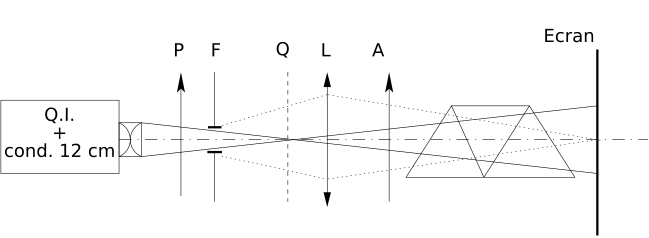
\includegraphics[width=5cm]{images-exp/spectrecannele.png}}
	\caption{Montage pour le spectre cannelé}
\end{figure}

On étudie, par exemple, une lame de quartz taillée parallèlement à l'axe optique.

    Réaliser le spectre d'une lampe quartz-iode à l'aide d'une fente F et d'un prisme à vision directe (on fera l'image de la fente sur l'écran à l'aide de la lentille, et on ajoutera ensuite le prisme à vision directe). Ajouter deux polariseurs croisés. Placer la lame Q entre P et A. Faire tourner Q dans son plan de manière à obtenir l'image la plus éclairée. Observer le spectre cannelé. On vérifiera que la rotation de Q modifie l'éclairement mais ne modifie ni le contraste ni la position des cannelures.[3] À quelles longueurs d'onde correspondent les cannelures ? Combien d'entre elles s'attend-on à voir ?

ATTENTION: ni la lentille ni le prisme ni la lame Q ne doivent diaphragmer le faisceau.

    Interposer successivement deux filtres étalonnés ayant une largeur à mi-hauteur d'environ $10 nm$, pour repérer la position de deux cannelures. En admettant que la dispersion du quartz est négligeable sur le spectre visible, en déduire la valeur de $\Delta n = n_e - n_o$ , que l'on comparera à la valeur tabulée. Pour plus de précision, on peut aussi remplacer le prisme à vision directe par une fibre reliée à un spectromètre USB.
    Tourner l'analyseur de 90°. Expliquer qu'on observe le spectre complémentaire. L'expérience suivante permet de le mettre en évidence dans le cas d'une lame mince.

Spectre cannelé

Reprendre le montage du § I.1.b en remplaçant la lame biréfringente par un canon de quartz. Régler l'orientation du canon de quartz de façon à avoir des franges bien rectilignes.

Observations

    Montrer qu'une rotation du canon dans son plan ne perturbe pas le phénomène.
    Qu'observe-t-on si l'on tourne l'analyseur ? En déduire le sens du pouvoir rotatoire.
    Noter les différences qualitatives avec le spectre cannelé observé en biréfringence.

Mesure

    Repérer la position de deux longueurs d'onde en utilisant des filtres interférentiels. Déterminer de quel angle il faut tourner l'analyseur pour faire passer une cannelure noire de $\lambda_{1}$ à $\lambda_{2}$.
    En déduire la constante de proportionnalité de la loi de Biot ( $\alpha \propto e/\lambda^{2}$ ).

\subsection{Pouvoir rotatoire}

\subsubsection{Effet Faraday}

Marche bien, utiliser le gros électroaimant.

Certaines substances acquièrent un pouvoir rotatoire lorsqu'elles sont soumises à un champ magnétique $B$ parallèle à la direction de la lumière qui les traverse. L'angle de rotation $\alpha$ est proportionnel à $B$.

Application : modulateur de Faraday, isolateur optique (voir notice de l'isolateur).

Principe

Une bobine entoure un barreau de verre à fort effet Faraday. Sous l'action du courant résultant d'une tension V appliquée à la bobine, il se produit un phénomène de polarisation rotatoire magnétique, c'est-à-dire que la polarisation linéaire d'un faisceau lumineux traversant le dispositif tourne d'un angle $\alpha$ proportionnel au champ magnétique produit par la bobine, donc proportionnel à V.

Utilisation

La notice indique le branchement du modulateur et décrit une expérience possible. La consulter. Étant donnée la faible ouverture du dispositif, ne l'utiliser que pour de la lumière laser. Le modulateur doit être éclairé par de la lumière polarisée linéairement ; mettre un polariseur à son entrée si le laser n'est pas polarisé. L'effet de rotation est faible ( $\alpha \approx 1^{\circ}$ pour quelques volts). Appliquer une tension alternative (GBF + ampli de puissance) 1<V<10 V.

L'angle que fait la polarisation avec l'analyseur est, sous l'effet du champ de fréquence $\omega$,
\[ \alpha=\alpha_0+\alpha_1\cos\omega t\equiv \alpha_0 + \alpha_1(t)\]

L'angle $\alpha_0$ peut être modifié en changeant l'orientation de l'analyseur. L'intensité après l'analyseur est
\[ I=I_0\cos^2(\alpha_0+\alpha_1(t)) = \frac{I_0}{2}\left[1+\cos(2\alpha_0 + 2\alpha_1(t))\right]\]

La variation d'intensité avec $\alpha_1(t)$, et donc l'amplitude du signal enregistré, est alors la plus grande pour $\alpha_0=\pi/4$, i.e. là où le cosinus s'annule : c'est en ce point que la pente de la sinusoïde est maximale, soit que $dI/d\alpha$ est maximal. On ne cherchera donc pas à annuler l'intensité à tension nulle ! (On réglera l'analyseur pour observer la moitié de l'intensité maximale.)

Remarque : La résistance de la bobine est faible, son impédance est uniquement selfique, et il est donc DANGEREUX pour l'appareil de lui appliquer une tension continue qui le ferait chauffer excessivement. Le modulateur est en fait uniquement adapté à la modulation de la polarisation d'un faisceau lumineux par une tension alternative.

Remarque importante

Lors d'un montage, l'expérience peut aussi être menée en utilisant un matériau avec une polarisation rotatoire induite (du flint) placé dans un électroaimant (cf. Sextant). On choisit des pièces tronc-coniques creuses pour pouvoir faire passer le faisceau laser dans l'électro-aimant, qui va traverser le milieu de pouvoir rotatoire variable, et on croise entre deux polariseurs. Les deux polariseurs sont croisés en champ nul et on a extinction. Lorsqu'on applique un champ magnétique, il faut tourner l'analyseur pour retrouver l'extinction. Cet angle permet de remonter au pouvoir rotatoire induit du matériau, et donc à sa constante de Verdet ( $\beta = \mathcal{V}eB$ ). On peut aussi étudier la variation de la constante de Verdet avec la longueur d'onde en changeant de laser. 

\section{Polarisation des ondes électromagnétiques.}
\underline{Références :}
\begin{itemize}
	\item Sextant
\end{itemize}

Polarisation : direction du chp dans le plan perpendiculaire à propagation.

\subsection{Caractère vectoriel des ondes EM}
Avec émetteur d'ondes centimétriques, et les deux cornets.Vérifier la loi de Malus

\subsection{Production d'onde EM polarisée}

[1P] \textit{Polarisation rectiligne}
Obtenue par dichroïsme: polaroïds

Un matériau est dit «dichroïque» si son absorption dépend de la polarisation de l'onde incidente.

Montage:


\begin{figure}
	\centerline{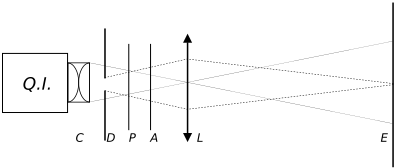
\includegraphics[width=5cm]{images-exp/Polarrectdichro.png}}
	\caption{Polarisation avec un matériau dichroïque}
\end{figure}

Faire l'image du trou D sur l'écran E avec la lentille L. Maintenir P fixe et vérifier l'extinction pour P et A croisés.

Remarque : En toute rigueur, on devrait utiliser un faisceau parallèle et ne contenant pas d'infrarouge (on dispose dans la collection de filtres antithermiques qui coupent l'infrarouge) car les polariseurs dont on dispose fonctionnent dans le visible mais très mal dans l'IR. Pour une expérience qualitative visuelle de cours, un faisceau quasi parallèle de lumière blanche convient. En revanche, pour une expérience quantitative et dans le cas de l'utilisation d'un capteur sensible aux infrarouges comme la photodiode, l'utilisation du filtre antithermique est indispensable.
Obtenue par réflexion vitreuse (interface air/diélectrique)

On utilise un miroir de verre noir, qui consiste en un diélectrique (du verre) dont la face arrière est peinte en noir et absorbe la lumière : ainsi, seule l'interface air/verre de la face avant est réfléchissante. Pour le réglage et l'utilisation, se reporter au mode d'emploi.

Envoyer un faisceau parallèle de lumière blanche sur le miroir $M_{1}$ et étudier la polarisation du faisceau réfléchi à l'aide d'un analyseur.

Pour une rotation complète de 360° de l'analyseur, l'intensité lumineuse présente 2 maxima et 2 minima placés à angle droit. Si l'incidence sur $M_{1}$ est l'incidence brewstérienne ($i=i_B$ avec $\tan i_{B}=n$, indice du verre), les minima sont nuls; on a affaire à de la polarisation rectiligne totale. Ici $i_{B} \approx 56^{\circ}$. Si $i \ne i_{B }$, la polarisation est rectiligne partielle, il subsiste, en plus de la vibration rectiligne précédente, une fraction de lumière naturelle. Dans les 2 cas, vérifier que la vibration rectiligne obtenue est perpendiculaire au plan d'incidence sur $M_{1}$.

Application : Contrôle rapide d'un polariseur. Observer l'image d'une lampe réfléchie sur une surface brillante diélectrique (peinture, bois verni, etc...) sous une incidence de l'ordre de 45°, à travers le polariseur à contrôler. Repérer l'angle du polariseur qui donne un minimum de luminosité. Interpréter. Ceci permet de voir si l'index du polariseur repère la transmission ou l'extinction, et si le polariseur n'a pas glissé par rapport à l'index.

Obtenue par diffusion

Lors de la diffusion de lumière non polarisée, la lumière réémise dans le plan perpendiculaire à la direction du faisceau incident est polarisée linéairement.
\begin{figure}
	\centerline{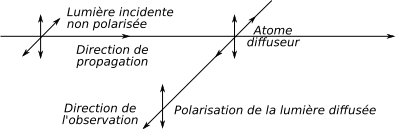
\includegraphics[width=5cm]{images-exp/Polardiffatom.png}}
	\caption{Polarisation par diffusion}
\end{figure}

Par beau temps, observer le ciel avec un polaroïd : il y a une extinction très nette pour une direction d'observation perpendiculaire aux rayons solaires (en déduire le rôle des filtres polariseurs sur les appareils photo).

Expérience :

\begin{figure}
	\centerline{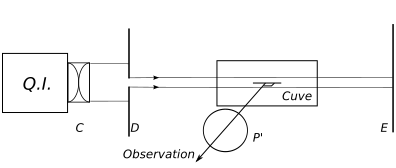
\includegraphics[width=5cm]{images-exp/Polarcuve.png}}
	\caption{Polarisation avec une cuve contenant du lait en poudre}
\end{figure}

On opère avec une cuve parallélépipédique en verre. Dans la cuve pleine d’eau ajouter une pincée de lait en poudre (pour le début de l'expérience il en faut très peu, l'eau doit être à peine diffusante).

Montrer l’état de la lumière diffusée à 90° avec un polariseur P' de grande taille placé contre la cuve.

On place un polariseur P sur le faisceau incident et on observe toujours à 90° à travers P'. Qu'observe-t-on en tournant P ?

Revenir à l'expérience initiale, ajouter suffisamment de lait pour que l'eau deviennent blanchâtre, mais on doit encore distinguer les objets vus à travers. Vérifier à travers P' que le degré de polarisation (c'est-à-dire le contraste entre les minima et maxima d'intensité) diminue, l'interpréter en terme de diffusions multiples.

Enfin observer sur l'écran E le changement de couleur du faisceau transmis, expliquer le phénomène.

\textit{Polarisation elliptique}

Rappels sur les lames cristallines (se référer à la bibliographie pour une introduction plus complète) :

Nous disposons de deux sortes de lames à faces parallèles de quartz:

quartz $\parallel$ : l'axe optique est parallèle aux faces de la lame.

quartz $\perp$ : l'axe optique est perpendiculaire aux faces de la lame.

Si on attaque une lame de quartz parallèle en incidence normale, la vitesse de propagation n'est pas la même pour une onde polarisée parallèlement à l'axe optique (indice $n_e$) et pour une onde polarisée perpendiculairement à l'axe optique (indice $n_o$). C'est le phénomène de biréfringence, qui donne lieu, en incidence non normale, à l'apparition de deux rayons réfractés (faire un schéma).

Dans le cas d'un quartz $\perp$, la biréfringence n'apparaît pas en incidence normale (ces lames seront utilisées pour l'étude de la polarisation rotatoire dans le TP Polarisation II).

Nous disposons aussi de lames de spath $\parallel$ (milieu uniaxe ne présentant pas de polarisation rotatoire).

Pour le quartz $\Delta n = n_e - n_o \approx 1 \times 10^{- 2}$. Pour le spath, $n_e - n_o \approx -20\times 10^{-2}$.

Il existe d'autre part des lames de mica, milieu biaxe sans polarisation rotatoire qui se comporte dans les géométries utilisées comme un milieu uniaxe.


\begin{itemize}
\item Lampe Mercure + polariseur + lame quart d'onde
\item Réflexion vitreuse à l'incidence de Brewster
\end{itemize}

\begin{figure}
	\centerline{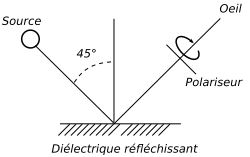
\includegraphics[width=5cm]{images-exp/Polarreflvitrbase.png}}
	\caption{Polarisation par réflexion vitreuse}
\end{figure}
\begin{figure}
	\centerline{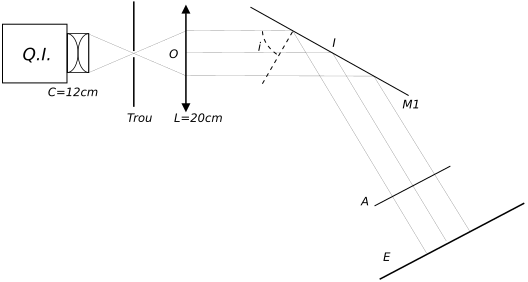
\includegraphics[width=5cm]{images-exp/Polarreflvitr.png}}
	\caption{Polarisation par réflexion vitreuse}
\end{figure}

\subsection{Analyse d'une lumière polarisée elliptiquement}
source : Laser polarisé+polariseur+onde $\lambda /4$
avec deuxième $\lambda /4$ et analyseur tournant, mesure du taux d'ellipticité.

\textit{Analyse de la lumière naturelle}

On peut utiliser une lampe Quartz-Iode.

Symétrie de révolution

Placer un polariseur sur le trajet du faisceau et montrer qu'en le faisant tourner, l'intensité reste constante. A ce stade la vibration est soit non polarisée, soit de polarisation circulaire totale ou partielle.
Absence de polarisation

Ajouter avant le polariseur une lame $\lambda / 4$ avec un filtre adapté et vérifier que l'intensité obtenue en faisant tourner le polariseur est toujours constante.

La lumière naturelle n'est donc pas polarisée (pour l'interprétation, voir le paragraphe III).


[1P] \textit{Méthode générale}

L'analyse complète d'une vibration lumineuse nécessite d'abord de déterminer s'il s'agit de lumière naturelle ou polarisée (totalement ou partiellement). Dans ce dernier cas, il faut déterminer le taux de polarisation. Si la lumière est polarisée, il faut déterminer si cette polarisation est rectiligne (et dans ce cas déterminer sa direction), circulaire ou elliptique (dans ces deux derniers cas, il faut déterminer l'orientation des axes et le sens droit ou gauche. Pour une polarisation elliptique, il faut enfin déterminer le rapport des deux axes de l'ellipse).

En présence d'une polarisation inconnue on procèdera comme indiqué dans le schéma de la dernière page avec les notations ci-dessous (voir également Duffait, Chap. IX-3) :
PolarisationAnalyseLegende.svg
\begin{figure}
	\centerline{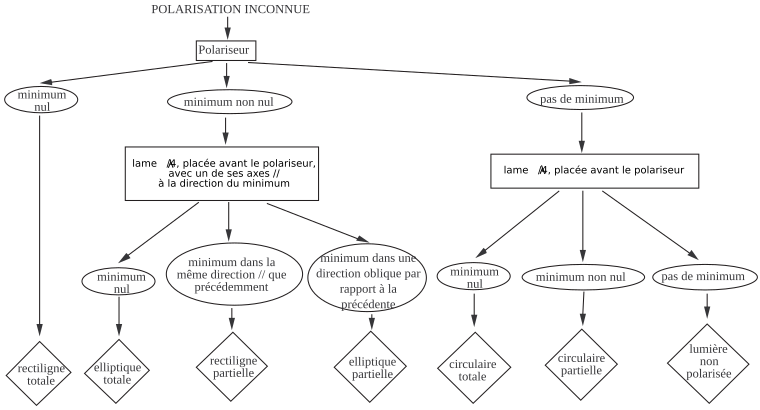
\includegraphics[width=10cm]{images-exp/PolarisationSchemaAnalyse.png}}
	\caption{Méthode d'analyse d'une lumière polarisée}
\end{figure}


Analyseur à extinction, type polaroïd ou nicol

Effectuer le montage suivant, à l'aide d'une lampe à vapeurs de mercure.


PolarisationPhiloraAnalyseur.svg


La détermination de l'extinction se fera soit visuellement, soit en utilisant une photodiode auto-alimentée[1]. Évaluer l'incertitude sur la détermination de la direction de la polarisation rectiligne dans ces deux cas.

Dans la suite, on pourra distinguer les extinctions ou les minima à l’œil nu, c'est suffisant dans le cadre de ce TP. Il est cependant toujours possible d'utiliser des photodiodes, notamment dans le cadre d'un montage. Dans le cas d'une détermination visuelle directe, il faut systématiquement repérer le minimum de luminosité, et pas le maximum, car l’œil y est plus sensible[2].
Pointé précis de la direction de polarisation

Analyseur à pénombre 
    L'instrument "traditionnel" destiné à faire des pointés précis de la direction absolue (c'est-à-dire par rapport à un repère du laboratoire) est l'analyseur à pénombre. Il n'est plus très utilisé aujourd'hui. Pour sa description voir Bruhat § 278 et suivants.

Polariseur tournant 
    Ref: Sextant p. 301 et suivantes.

PolarisationPolariseurTournant.svg

Un polariseur de type polaroïd a été monté sur le moteur d'un hacheur optique. Une petite languette de scotch noir est collée sur le bord du disque dans la direction de l'axe absorbant du polariseur. Son passage dans la fourche optique permet au boîtier du hacheur de fournir une tension de référence (sortie « reference out ») dont le zéro correspond au passage de l'axe absorbant dans la direction (généralement) verticale. On notera que la taille de cette languette limite déjà la précision du pointé.

Envoyer sur ce polariseur tournant le faisceau d'un laser polarisé. Observer l'évolution temporelle de l'intensité émergente avec une photodiode et un oscilloscope numérique.

Loi de Malus 
    Faire une acquisition de ce signal et l'ajuster par une sinusoïde. Commenter en particulier la période et la valeur moyenne. Pourquoi la loi de Malus illustre-t-elle le caractère vectoriel de la lumière ?

Pointé d'une direction de polarisation 
    Mesurer la phase du signal par rapport au signal de référence. En déduire la direction de polarisation. Quelle précision peut-on attendre pour un tel pointé absolu de la direction de polarisation ? Introduire une lame  $\lambda /2$ avant le polariseur tournant. Constater que la polarisation reste rectiligne. Tourner cette lame d'un angle arbitraire. Déduire de la courbe lue à l'oscilloscope la rotation de la direction de polarisation induite. Conclure. Quelle précision peut-on attendre de la méthode du polariseur tournant pour des pointés relatifs de direction de polarisation ?

    [1P] \textit{Analyse d'une vibration elliptique}

Produire un faisceau de lumière polarisée elliptiquement par l'une des méthodes proposées au II.2.

Repérer avec un analyseur la direction de l'intensité minimale (petit axe de l'ellipse), puis ôter l'analyseur. Placer une lame quart d'onde (et donc travailler en lumière monochromatique) de manière à ce que son axe lent coïncide avec la direction que l'on vient de repérer.

A la sortie de la lame quart d'onde, on a alors une vibration rectiligne. Replacer l'analyseur avec son orientation initiale et repérer l'extinction en tournant l'analyseur d'un angle $\beta < \pi /4$.

L'angle $\beta$ dont on a dû tourner l'analyseur permet d'avoir :

    le degré d'ellipticité de la vibration par $\tan \beta = b/a$ où $a$ est le demi grand axe de l'ellipse ( $b$ est le demi petit axe)
    le sens de rotation de la vibration (opposé au sens de rotation de l'analyseur)

Faire les calculs qui permettent de trouver ces résultats.

Polariseur tournant 
    Envoyer la lumière polarisée elliptiquement sur le polariseur tournant décrit au paragraphe précédent. Comment déduire le degré d'ellipticité de la courbe obtenue à l'oscilloscope ?

    [2P] \textit{Cas d'une vibration rectiligne partielle}

Le moyen de production le plus simple consiste à utiliser la réflexion vitreuse d'un faisceau non polarisé avec une incidence autre que l'incidence de Brewster (cf. II.1.b). On peut aussi utiliser une pile de glace par transmission (cf. II.1.b).

Pour l'analyser, repérer la direction de l'intensité minimale grâce à un analyseur, qu'on retire ensuite.

Placer une lame $\lambda/4$ (et donc travailler en lumière monochromatique) dont l'un des axes est parallèle à la direction repérée précédemment. Avec l'analyseur, vérifier que le minimum d'intensité (non nul) est parallèle à l'un des axes de la lame. En déduire que la vibration est rectiligne partielle (on ne propose pas d'aller plus loin dans l'analyse). Qu'aurait-on observé si la vibration obtenue avait été elliptique totale ? Et si elle avait été elliptique partielle ?


Prendre l'habitude de mettre systématiquement un filtre anti-thermique dans ce cas, on rappelle que les analyseurs ne filtrent pas les infrarouges.
L'œil est un récepteur dont la sensibilité est approximativement logarithmique.
\section{Production et mesure de champs magnétiques.}
\underline{Références :}
\begin{itemize}
	\item Sextant
\end{itemize}
\subsection{Mesure du champ magnétique terrestre, boussole (méthode des tangentes)}
Attention nombreuses sources de bruit
Marche bien.

La boussole des tangentes est un dispositif simple permettant d'obtenir une estimation de la valeur de la composante horizontale du champ magnétique terrestre. Elle est constituée d'une grande bobine plate, verticale, comportant N spires de rayon R, au centre de laquelle est placée une aiguille aimantée sur un support horizontal. Le dispositif permet de choisir le nombre de spires de la bobine (de N=1 à N=5). Attention, ces spires sont de rayons différents. En pratique, on utilisera une seule spire dont on choisira le rayon le plus adapté pour la manipulation.
Principe de la mesure

La boussole indique la direction du champ magnétique local. Le principe consiste à mesurer la déviation de l'aiguille lorsqu'un champ magnétique est appliqué à l'aide de la spire. Le champ généré par la spire étant connu, il est alors possible de remonter à l'amplitude de la composante horizontale du champ magnétique terrestre. La boussole n'est sensible qu'au champ magnétique contenu dans son plan. Dans la suite, on ne considérera donc que la composante horizontale du champ (notée $\mathbf{B}_{Terre}$).

Pour cela, orienter la boussole des tangentes afin que l'aiguille, en l'absence de courant dans les spires, pointe dans le plan de la bobine. Dans cette configuration, $\mathbf{B}_{Terre}$ est orthogonal au champ généré par la spire noté $\mathbf{B}_{0}$. La déviation de l'aiguille $\alpha$ permet de repérer la direction du champ total $\mathbf{B}_{tot}=\mathbf{B}_{Terre}+\mathbf{B}_{0}$.
\begin{figure}
	\centerline{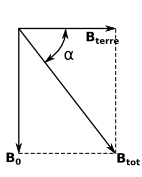
\includegraphics[width=5cm]{images-exp/Boussole_tangente.png}}
	\caption{Principe de la boussole}
\end{figure}

Pour une spire de rayon R, parcourue par un courant I, le champ généré au centre de la spire vaut
$\mathbf{B}=\frac{\mu_0 I}{2R}$.

Ainsi, la déviation est reliée simplement à $B_{Terre}$ selon
$\tan \alpha=\frac{\mu_0 I}{2 R B_{Terre}}$.
Manipulation

À partir de l'ordre de grandeur du champ magnétique terrestre, et sachant que le courant maximal admissible par une spire est de $5 A$ !, choisir le rayon de spire le mieux adapté pour observer une déviation notable.

À l'aide d'une alimentation continue et d'un ampèremètre, mesurer la déviation $\alpha$ en fonction du courant $I$. Quel est le paramètre dont l'incertitude domine dans la mesure ? On prendra soin de l'estimer soigneusement pour chaque mesure.

À l'aide d'un ajustement avec QtiPlot, en déduire la valeur de la composante horizontale du champ terrestre. Commenter.

Quel intérêt y a-t-il à prendre des valeurs négatives et positives du courant I pour la mesure ? Doit-on modifier alors la fonction d'ajustement de $\alpha(I)$ ? et si oui, comment ?
Remarques

Étant donné les champs rémanents pouvant exister, notamment au niveau des tables métalliques, il peut être bon de vérifier que la boussole indique bien le nord, par exemple en prenant une autre boussole et en s'assurant que les deux pointent dans la même direction. Si ce n'est pas le cas, essayer de déplacer la boussole des tangentes dans la pièce.

On ne connait le champ magnétique créé par une spire que sur son axe. Ainsi, assimiler le champ magnétique auquel est soumis l'aiguille au champ au centre est une approximation, dont il convient d'apprécier l'extension.

Par ailleurs, il convient de noter que la formule donnant l'angle de déviation est exacte précisément parce qu'elle correspond à l'équilibre entre deux couples de sens opposés. Par chance, le couple subi par un moment magnétique est linéaire en le champ appliqué.

Enfin, ne pas oublier que l'aiguille est fabriquée dans un matériau ferromagnétique. Lorsqu'un champ est appliqué, ce matériau réagit en développant lui-même un (petit) champ magnétique. Sachez apprécier la petitesse de celui-ci par rapport au champ ambiant. 

\subsection{Bobines de Helmoltz}

On utilise deux bobines circulaires identiques, de rayon R, qui peuvent coulisser parallèlement à leur axe sur des rails, et dont l'écartement D est mesurable.

À l'aide d'un teslamètre (à effet Hall) dont la géométrie permet de déplacer la sonde sur l'axe des bobines en repérant sa position, tracer point par point la courbe donnant le champ magnétique sur l'axe dans différents cas :

    une bobine seule,
    les 2 bobines à distance quelconque,
    les 2 bobines réglées en configuration Helmholtz : $D = R$ (Les branchements doivent être faits tels que les bobines créent des champs magnétiques de même sens. Dans le cas contraire, on parle de configuration anti-Helmholtz.). Que peut-on dire du champ entre les deux bobines ?

Rappel : pour une bobine (considérée plate, à vérifier dans les conditions de l'expérience) possédant N spires, et en notant $\theta$ l'angle entre l'axe de la bobine et la droite joignant le point M à la bobine, on a

\[\vec B = \frac{\mu_0 NI}{2 R}\sin^3(\theta) \vec{u_z}\]

Lorsque les dimensions de la bobines ne permettent pas de l'assimiler à une bobine plate, on privilégiera la formule du solénoïde fini.

Remarque : Il est possible d'automatiser cette mesure en utilisant une table traçante, sur laquelle on aura fixé la sonde à effet Hall. Ne pas effectuer cette manipulation dans un premier temps, mais on pourra la mettre en place pendant la période de préparation des ora

\subsection{Mesure du champ magnétique dans l'entrefer d'un électroaimant}
Fluxmètre, sonde à effet Hall (comparer)

Électroaimant : une source fiable de forts champs magnétiques

Un électroaimant est un exemple de circuit magnétique ouvert. Il est composé de grosses bobines de cuivre dans lesquelles on a placé un élément de fer formant presque un circuit fermé. On propose d'étudier le champ magnétique dans l'entrefer.

Démontrer, en utilisant le théorème d'Ampère et la conservation du flux magnétique, que :
\[ B \approx \frac{\mu_0 n I}{\frac{L}{\mu_r}\frac{s}{S} + e}  \qquad\qquad\qquad\qquad(1)\]

Le circuit étant ferromagnétique, on peut poser en absence de saturation que $\mu_r \gg 1$, d'où :
\[ B \approx \frac{\mu_0 nI}{e} \qquad\qquad\qquad\qquad(2)\]

Voir la notice de l'électroaimant. Attention, les deux bobines de 5600 spires sont en parallèle et sont donc équivalentes à 11200 spires parcourues par le courant moitié.
\begin{figure}
	\centerline{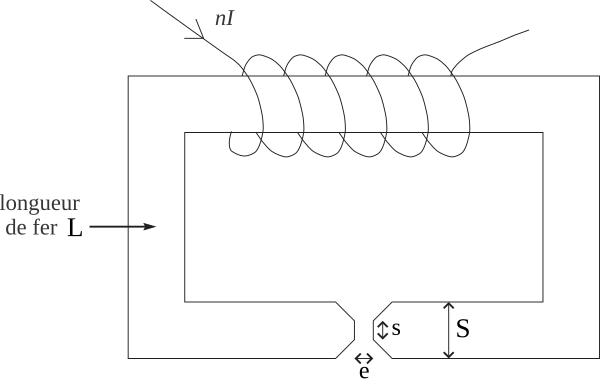
\includegraphics[width=10cm]{images-exp/MagnetismeCircuitMagnetique.png}}
	\caption{Schéma d'un électroaimant}
\end{figure}

Réaliser les expériences décrites ci-dessous avec les pièces polaires tronconiques (s/S = 1/4):

    c'est la configuration qui permet d'atteindre les champs les plus grands, ce qui est intéressant à étudier.
    c'est celle où le passage de (1) à (2) a le plus grand domaine de validité en e (par le terme s/S). 

(les pièces polaires cylindriques seront utilisées lorsque l'on cherchera un grand domaine de champ uniforme). On fera varier l'épaisseur e entre environ 1 cm (afin de pouvoir glisser la sonde à effet Hall) et 4 cm (diamètre des pièces polaires). On limitera le courant à 4 A (5 A en régime non permanent).

Commencer par faire un calcul d'ordre de grandeur de $ \frac{L}{\mu_r}\frac{s}{S}$ sachant que $L \simeq 1,40 m$ (à vérifier) et qu'on a typiquement $\mu_r > 1000$. Conclure.

Courbe $B = f(I)$ à $e$ constant:

Mesurer $B$ en fonction de $I$ en prenant la plus petite valeur de $e$.
La courbe commence par une zone linéaire. Interpréter et en déduire le nombre de spires.
Comment peut-on expliquer que la courbe s'incline pour les fortes intensités ? En déduire un ordre de grandeur de $\mu_r$ à l'intensité maximale (la valeur de $\mu_r$ à faible intensité n'est pas mesurable ici).

Courbe $\frac{1}{B} = f(e)$ à $I$ constant:

Mesurer B en fonction de e en prenant une faible valeur de I afin de travailler à coup sûr loin de la saturation (1 A au maximum comme on peut le voir sur la notice p.9).
Pour vérifier l'expression (1), représenter $1/B$ en fonction de e. Faire un ajustement linéaire. Cette loi est-elle validée ? De la pente déduire le nombre de spires.
De l'ordonnée à l'origine on peut en déduire $\mu_r$, cependant l'expérience montre que ceci conduit le plus souvent à un résultat absurde : il n'est pas rare de trouver une valeur de $\mu_r$ négative ou nettement inférieure à 1000. En réalité la formule (1) est approchée et de plus $\mu_r$ subit des variations complexes, même en faible courant, ce qui perturbe gravement la faible ordonnée à l'origine même si les points semblent convenablement alignés. Un choix raisonnable des incertitudes doit conduire à la possibilité d'une ordonnée à l'origine nulle, ce qui traduit le fait que $\mu_r$ est trop grand pour pouvoir être déterminé ici. En déduire que dans ces conditions le produit $Be$ est constant à $I$ donné.

On peut aussi s'intéresser qualitativement au domaine dans lequel le champ peut spatialement être considéré comme uniforme, en particulier lorsque e devient grand. 

L'effet Hall : les sondes les plus courantes sont les teslamètres à effet Hall, constitués essentiellement d'un capteur à effet Hall traversé par un courant constant, et d'un circuit d'amplification de la tension de Hall (consulter la notice) ;
effet inductif : en déplaçant une bobine exploratrice dans un champ magnétique non-uniforme, il se créé une f.é.m. à ses bornes. L'intégration de la f.é.m. induite dans la bobine donne la variation du flux du champ magnétique. On appelle ce capteur un fluxmètre. Cette intégration est réalisée avec un circuit à amplificateur opérationnel. La sensibilité de ce fluxmètre électronique est contrôlée en changeant la surface totale $ S $ de la bobine exploratrice. ;

ccl : différents odg => différentes méthodes
Mise à profit de l'induction, aimantation permanente et effet Hall

\section{Milieux magnétiques.}
\subsection{barreaux dans un champ magnétique}
Rappeler déf para, dia, ferro

Tous les matériaux sont magnétiques puisque constitués d'éléments présentant des moments magnétiques microscopiques. Ces moments peuvent provenir du spin des particules, ou d'une contribution orbitale. Si ces moments n'interagissent que faiblement, le matériau associé ne peut pas avoir d'aimantation spontanée (i.e., en l'absence de champ magnétique extérieur). De plus, la réponse magnétique de ce matériau à un champ extérieur est faible : il s'agit d'un système paramagnétique ou diamagnétique.

[1P] \textit{Mise en évidence (qualitatif)}

À l'aide d'un fil sans torsion, suspendre par le milieu un barreau diamagnétique ou paramagnétique dans l'entrefer d'un électroaimant. On observe les déplacements suivants :
MagnetismeBarreaux.svg

Le barreau diamagnétique se place dans les régions de champ faible, et le barreau paramagnétique dans les régions de champ fort. Il est nécessaire d'utiliser ici les pièces polaires coniques pour avoir de fortes inhomogénéités de champ : comment sont alors les lignes de champ ? 

\subsection{Mesure de la susceptibilité magnétique d'un milieu para}
tube FeCl3, montée dans électroaimant=> retrouver $\chi$, prendre le gros aimant de Cachan

Mesure de la susceptibilité d'un milieu paramagnétique

Référence : BFR, Électromagnétisme 4, chap. 6

Choisir les pièces polaires tronconiques (Pourquoi ?). Placer entre elles une branche d'un tube en U contenant une solution de FeCl3, de concentration et de masse volumique connues. On choisira un écartement de pôles assez faible mais sans risque de casse pour le tube (sachant que les entrefers se rapprochent lorsque l'électroaimant est en marche).

Mesurer la dénivellation produite par un champ magnétique en projetant sur un écran la branche située hors de l'entrefer, sur laquelle a été fixé un réglet transparent. Le but est de déterminer d'abord la susceptibilité de la solution, puis d'en déduire, assez grossièrement, la susceptibilité de $FeCl_3$ solide.
MagnetismeSusceptibiliteFeCl3.svg

Mesurer le champ dans l'entrefer à l'aide du teslamètre à effet Hall ; bien choisir le niveau d'affleurement dans l'état final du liquide au centre de l'entrefer. La susceptibilité de la solution est donnée (dans le système SI) par la relation :
\[ \chi {B^2\over 2\mu_0} = \rho g\; 2 \Delta h\]

(Refaire le calcul : que représente exactement B dans cette équation ? Pourquoi l'entrefer doit-il être centré sur la surface libre ? Éventuellement reprendre l'expérience en décalant le tube en U de plusieurs cm vers le haut.).
Remarque : il faut faire attention à la définition de $\chi$. Dans le système international d'unités, $\chi$ est un nombre sans dimension (il peut être pratique de le considérer comme un moment magnétique par unité de volume dans un champ de 1 A.m-1). On le calcule à partir de $\chi_{solide}$, la susceptibilité du solide, en appliquant une loi approchée d'additivité des moments magnétiques (loi de Wiedman) : cela suppose que les moments magnétiques n'interagissent pas. L'eau ne jouant qu'un rôle de dilution on a :
\[ \frac{\chi_{\rm solide}}{\chi_{\rm solution}}= \frac{\rho_{\rm solide}}{d\times \rho_{\rm eau} \times r}\]

où d est la densité de la solution et r le pourcentage en masse de $FeCl_3$ dans la solution (savoir retrouver cette formule, qui ne figure pas dans les livres).

En pratique, vérifier que le rôle de l'eau est négligeable, soit en mesurant, soit en calculant la déviation obtenue avec un tube identique contenant de l'eau pure. Les données pour la solution sont inscrites sur la bouteille. Les valeurs de $\chi_{FeCl_3}$ et de $\chi_{H_20}$ en SI sont données dans un des tableaux du Fleury-Mathieu, tome 6 (voir les index en fin d'ouvrage pour retrouver ce tableau).

\subsection{Transition ferro-para, mesure de la température de Curie}
cf plus haut
\section{Métaux.}
\underline{Références :}
\begin{itemize}
	\item Physique des solides, Ascroft
	\item Physique expérimentale, Fruchart
	\item Étude de la dynamique électronique des plasmas denses et tièdes par interférométrie optique, Deneuville
\end{itemize}

déf
\subsection{Mesure de la conductivité thermique du cuivre}
erreur systématique ?

Mesure de la conductivité thermique du cuivre

On dispose d'un montage contenant un barreau de cuivre dont la température est fixée à une extrémité par une circulation d'eau, et qui est chauffé à l'autre extrémité par une résistance de puissance de $47 \Omega$. Deux thermocouples sont insérés dans le barreau, distants de $100 mm$.

Faire passer une puissance de quelques watts dans la résistance de $47 \Omega$, et mesurer le gradient de température dans le barreau. Attendre l'établissement du régime permanent (il peut être intéressant d'estimer le temps caractéristique). En déduire la conductivité thermique du cuivre $\lambda$. Pour cela, on peut supposer que la puissance électrique fournie contribue entièrement au flux thermique à travers le barreau [2].

Analyse 

Rapprocher la valeur trouvée pour la conductivité thermique $\lambda$ de celle trouvée pour la conductivité électrique $\sigma$ (cf. TP Mesures électriques). La loi de Wiedemann-Franz (cf. Kittel, Physique de l'état solide) indique que : « pour les métaux à des températures pas trop basses, le rapport de la conductivité thermique à la conductivité électrique est directement proportionnel à la température, la valeur de la constante de proportionnalité étant indépendante du métal considéré. Ce résultat fut très important dans la théorie des métaux car il fut l'une des preuves du modèle du gaz d'électrons. » Comparer vos mesures à la valeur attendue pour le rapport
\[\frac{\lambda}{\sigma T} = \frac{\pi^2}{3}\left(\frac{k_B}{e}\right)^2 = 2.44\times 10^{-8}  \mathrm{S.I.}\]


\subsection{Mesure de la conductivité électrique du cuivre}

Nom de la manip : bobine de cuivre pur vernis.

Loi de Wiedeman-Franz

Conductivité électrique. Principe de la mesure à 4 points

Prendre un multimètre à 6 digit pour plus de précision. Utiliser un agitateur pour homogéneiser la température (à éteindre pendant la mesure). Faire varier beaucoup la température (avec une bouilloire/ de la glace) pour observer des variations significatives.

On dispose d'un long rouleau de fil de cuivre, de section $ S$ et longueur $L$ connues.
Principe de la mesure à 4 points

\begin{figure}
	\centerline{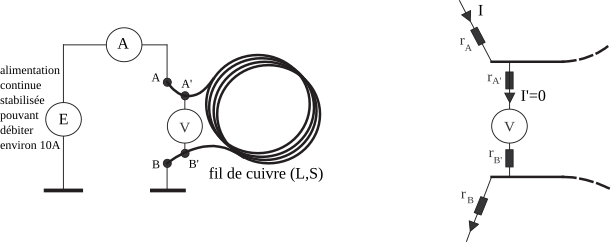
\includegraphics[width=10cm]{images-exp/CircuitElecMesure4Points.png}}
	\caption{Montage quatre points}
\end{figure}

La résistance de ce fil de cuivre étant très faible (quelques centièmes d'$\Omega$), on doit utiliser une méthode de mesure particulière: elle permet de s'affranchir de la résistance parasite des contacts et des fils de liaison. Le principe de cette mesure à 4 points est que les fils d'amenée du courant et de mesure de la tension ne soient pas connectés au même point du composant dont on veut mesurer la résistance. Sur la figure ci-dessus, on représente ces résistances parasites, et on voit que la mesure au voltmètre ne les fait effectivement pas intervenir puisque $r_{A'}$ et $r_{B'}$ sont parcourues par un courant I' négligeable devant le courant principal I.

Comparer les indications du voltmètre lorsqu'il est branché en A et B ou en A' et B', et en déduire un ordre de grandeur des résistances parasites.
Mesure de la conductivité électrique du cuivre

On peut accéder à la conductivité du cuivre en mesurant la résistance de ce fil. On pourra en montage effectuer cette mesure à différentes températures, en plongeant le fil dans un cristallisoir contenant de l'eau. Vérifier qu'on peut approximer localement la résistivité en fonction de la température par une loi affine : $\rho(T) = \rho(T_{0}) [1 + \alpha (T-T_{0})]$ (loi de Matthiessen).[2] Le coefficient $\alpha$, appelé coefficient de température, est donné dans le Handbook. 

\subsection{Mesure de la pulsation plasma de certains métaux}
Ruello et Edely p 19 à 28, prisme à revêtement métallique

Présentation théorique

Dans les métaux, il existe des ondes particulières dites ondes plasma, qui correspondent à une oscillation de la densité de charge. Ces ondes ayant une structure longitudinale (le vecteur d'onde est parallèle au champ électrique) elles ne peuvent pas être engendrées optiquement (structure transverse de l'onde électromagnétique). Cependant on peut lever cette contrainte à l'interface entre un métal et un diélectrique en générant une onde évanescente qui présentera une composante longitudinale. Le mode mixte lumière/oscillation plasma est alors appelé plasmon. Le couplage entre l'onde plasma et la lumière, n'est efficace que lorsqu'il y a accord des vitesses de phase des deux ondes, c'est-à-dire égalité de leur vecteurs d'onde le long de l'interface. Dans ces conditions, on a :
$n \sin \theta_p = \sqrt{\frac{\epsilon_1}{1+\epsilon_1}}$

n représente l'indice du verre, $\theta_p$ l'angle d'incidence de l'onde lumineuse sur l'interface verre/métal et $\epsilon_1$ la partie réelle de la constante diélectrique du métal. On a fait l'approximation $n_{air}=1$.

Lorsque cette condition est réalisée, il y a couplage efficace vers le plasmon, ce qui se traduit par une chute brutale de la lumière réfléchie pour cet angle d'incidence [3]. L'énergie transférée vers le plasmon est ensuite dissipée dans le métal. Cette dissipation, liée à la partie imaginaire de la constante diélectrique ($\epsilon_2$) se traduit par une certaine largeur de la résonance [4].
Manipulation et mesures

On dispose d'un prisme droit dont une des faces est couverte d'un film d'or de 50 nm d'épaisseur, que l'on peut monter sur le plateau tournant d'un goniomètre.
Manipulation qualitative

On éclaire le prime avec un faisceau laser élargi par une lentille de très courte focale et polarisé à l'aide d'un polariseur. De la sorte, la face métallique est éclairée sous tout un ensemble d'incidences. Celle pour laquelle la condition de couplage au plasmon de surface est réalisée, sera caractérisée par un coefficient de réflexion nul. Sur un écran placé en sortie on observe une raie noire au milieu de la tache de lumière réfléchie. Vérifier que cette raie n'existe que pour une polarisation p (qui est ici horizontale). Pour prouver que ce phénomène est lié à la couche métallique, on peut faire la contre expérience à l'aide du second prisme, identique au premier si ce n'est l'absence de couche métallique.
Mesure de la constante diélectrique de l'or

On éclaire le prisme avec un laser Hélium-Néon suivi d'un polariseur et on observe la lumière réfléchie à l'aide d'un écran ou bien à l'aide d'un ensemble lentille/photodiode si on veut faire une étude quantitative du coefficient de réflexion.


Dispositif pour l'observation de la résonance plasmon de surface.


On commencera par repérer l'incidence normale sur la face d'entrée du prisme en renvoyant la lumière partiellement réfléchie par celle-ci sur le laser. Ensuite on tourne le plateau jusqu'à extinction. En déduire l'angle d'incidence sur la face métallisée $\theta_p$ (Il faut tenir compte de la réfraction sur le dioptre air/verre).

Il faut alors mesurer précisément la valeur de l'indice du verre composant le prisme. On notera que pour un prisme droit, il n'existe pas d'angle de minimum de déviation si l'indice du verre est supérieur à $\sqrt{2}$, ce qui est le cas ici. On pourra néanmoins mesurer cet indice en repérant l'angle de Brewster sur une de ses faces : $\tan \theta_b=n_v$.

Muni de ces valeurs on peut alors estimer la partie réelle de la constante diélectrique de l'or à 633 nm.

En utilisant l'expression simplifiée de la constante diélectrique donnée par le modèle de Drüde, on peut estimer un ordre de grandeur de la densité d'électrons libres.
$\epsilon_1 \simeq 1- \frac{\omega_p^2}{\omega^2} avec \omega_p^2=\frac{ne^2}{m \epsilon_0}$

L'écart à la valeur tabulée (de la densité électronique) provient de la contribution des électrons de coeur à la constante diélectrique mesurée.

N.B. La valeur tabulée de la constante diélectrique à 632,9 nm est $\epsilon_1=-11,8$, $\epsilon_2=1,25$. Valeur tabulée de la densité d'électrons de conduction : $n_c=5,9\cdot10^{28} m^{-3}$



ccl : différentes ptés des métaux, liées à la présence d'un gaz d'électrons

\section{Matériaux semi-conducteurs.}

def

\subsection{Influence de l'éclairement}
Avec l'illuminateur monochromatique, mesure du seuil d'absorption et estimation de l'énergie de gap.

cf plus haut
\subsection{Influence de la température}
Mesure de R(T), détermination de l'énergie de gap (normalement plus précise)

L'observation, à température ordinaire, de la conduction intrinsèque requiert un semiconducteur non dopé. On propose ici d'étudier un barreau de Germanium non dopé [1].

Une résistance chauffante est accolée à l'échantillon. Elle doit être alimentée sous 6 V et 5 A maximum. On utilisera de préférence une alimentation variable : il est conseillé de procéder à un chauffage lent de l'échantillon en appliquant au départ une tension de 2 V, puis de 4 V et enfin de 6 V.

La température est donnée par un thermocouple de type T (cuivre-constantan), dont la soudure est collée à l'échantillon. Sa sensibilité est de $40 \mu V/K$. Utiliser pour la lecture de la f.e.m. du thermocouple un voltmètre de sensibilité appropriée (affichant 0,01 mV). Attention de ne pas dépasser 150°C, soit une f.e.m. de 5 mV pour le thermocouple ! \[5 mV=40 \mu V/K \times (150°C-25°C)\]

\begin{figure}
	\centerline{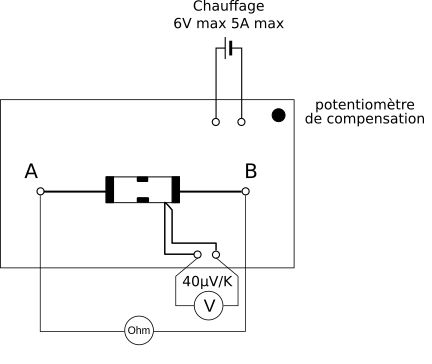
\includegraphics[width=10cm]{images-exp/Semicon3b.png}}
	\caption{Plaquette semiconducteur}
\end{figure}

À l'aide d'un ohmmètre, mesurer la variation de la résistance R avec la température T. Pourquoi est-il préférable de faire les mesures lors du refroidissement ? Déduire du diagramme $\ln R = f(1/T)$ la largeur de la bande interdite du germanium.

Remarque : On pourra aussi étudier une thermistance du commerce. La plage d'utilisation est limitée à -25°C,+125°C. Mesurer à l'ohmmètre sa résistance pour différentes températures dans ce domaine, en la trempant dans un ballon d'eau à différentes températures. Il est nécessaire d'agiter pour homogénéiser la température. Construire la courbe $\ln \left( R \right) = f\left( 1/T \right)$ et la comparer à la notice du constructeur (notice 5). 

\subsection{Effet Hall : mesure du nombre de porteurs de charges}

Effet Hall
\begin{figure}
	\centerline{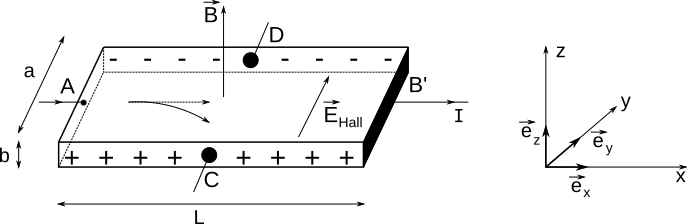
\includegraphics[width=10cm]{images-exp/Semicon5.png}}
	\caption{Principe de l'effet Hall}
\end{figure}

Le dessin représente le cas q>0.

Lorsque le barreau est plongé dans un champ magnétique $\vec{B} \parallel Oz ( \vec{B} = B\,\vec{e}_z$) et parcouru par un courant I longitudinal parallèle à Ox, il apparaît un champ électrique transversal parallèle à Oy, dit champ de Hall.
\begin{figure}
	\centerline{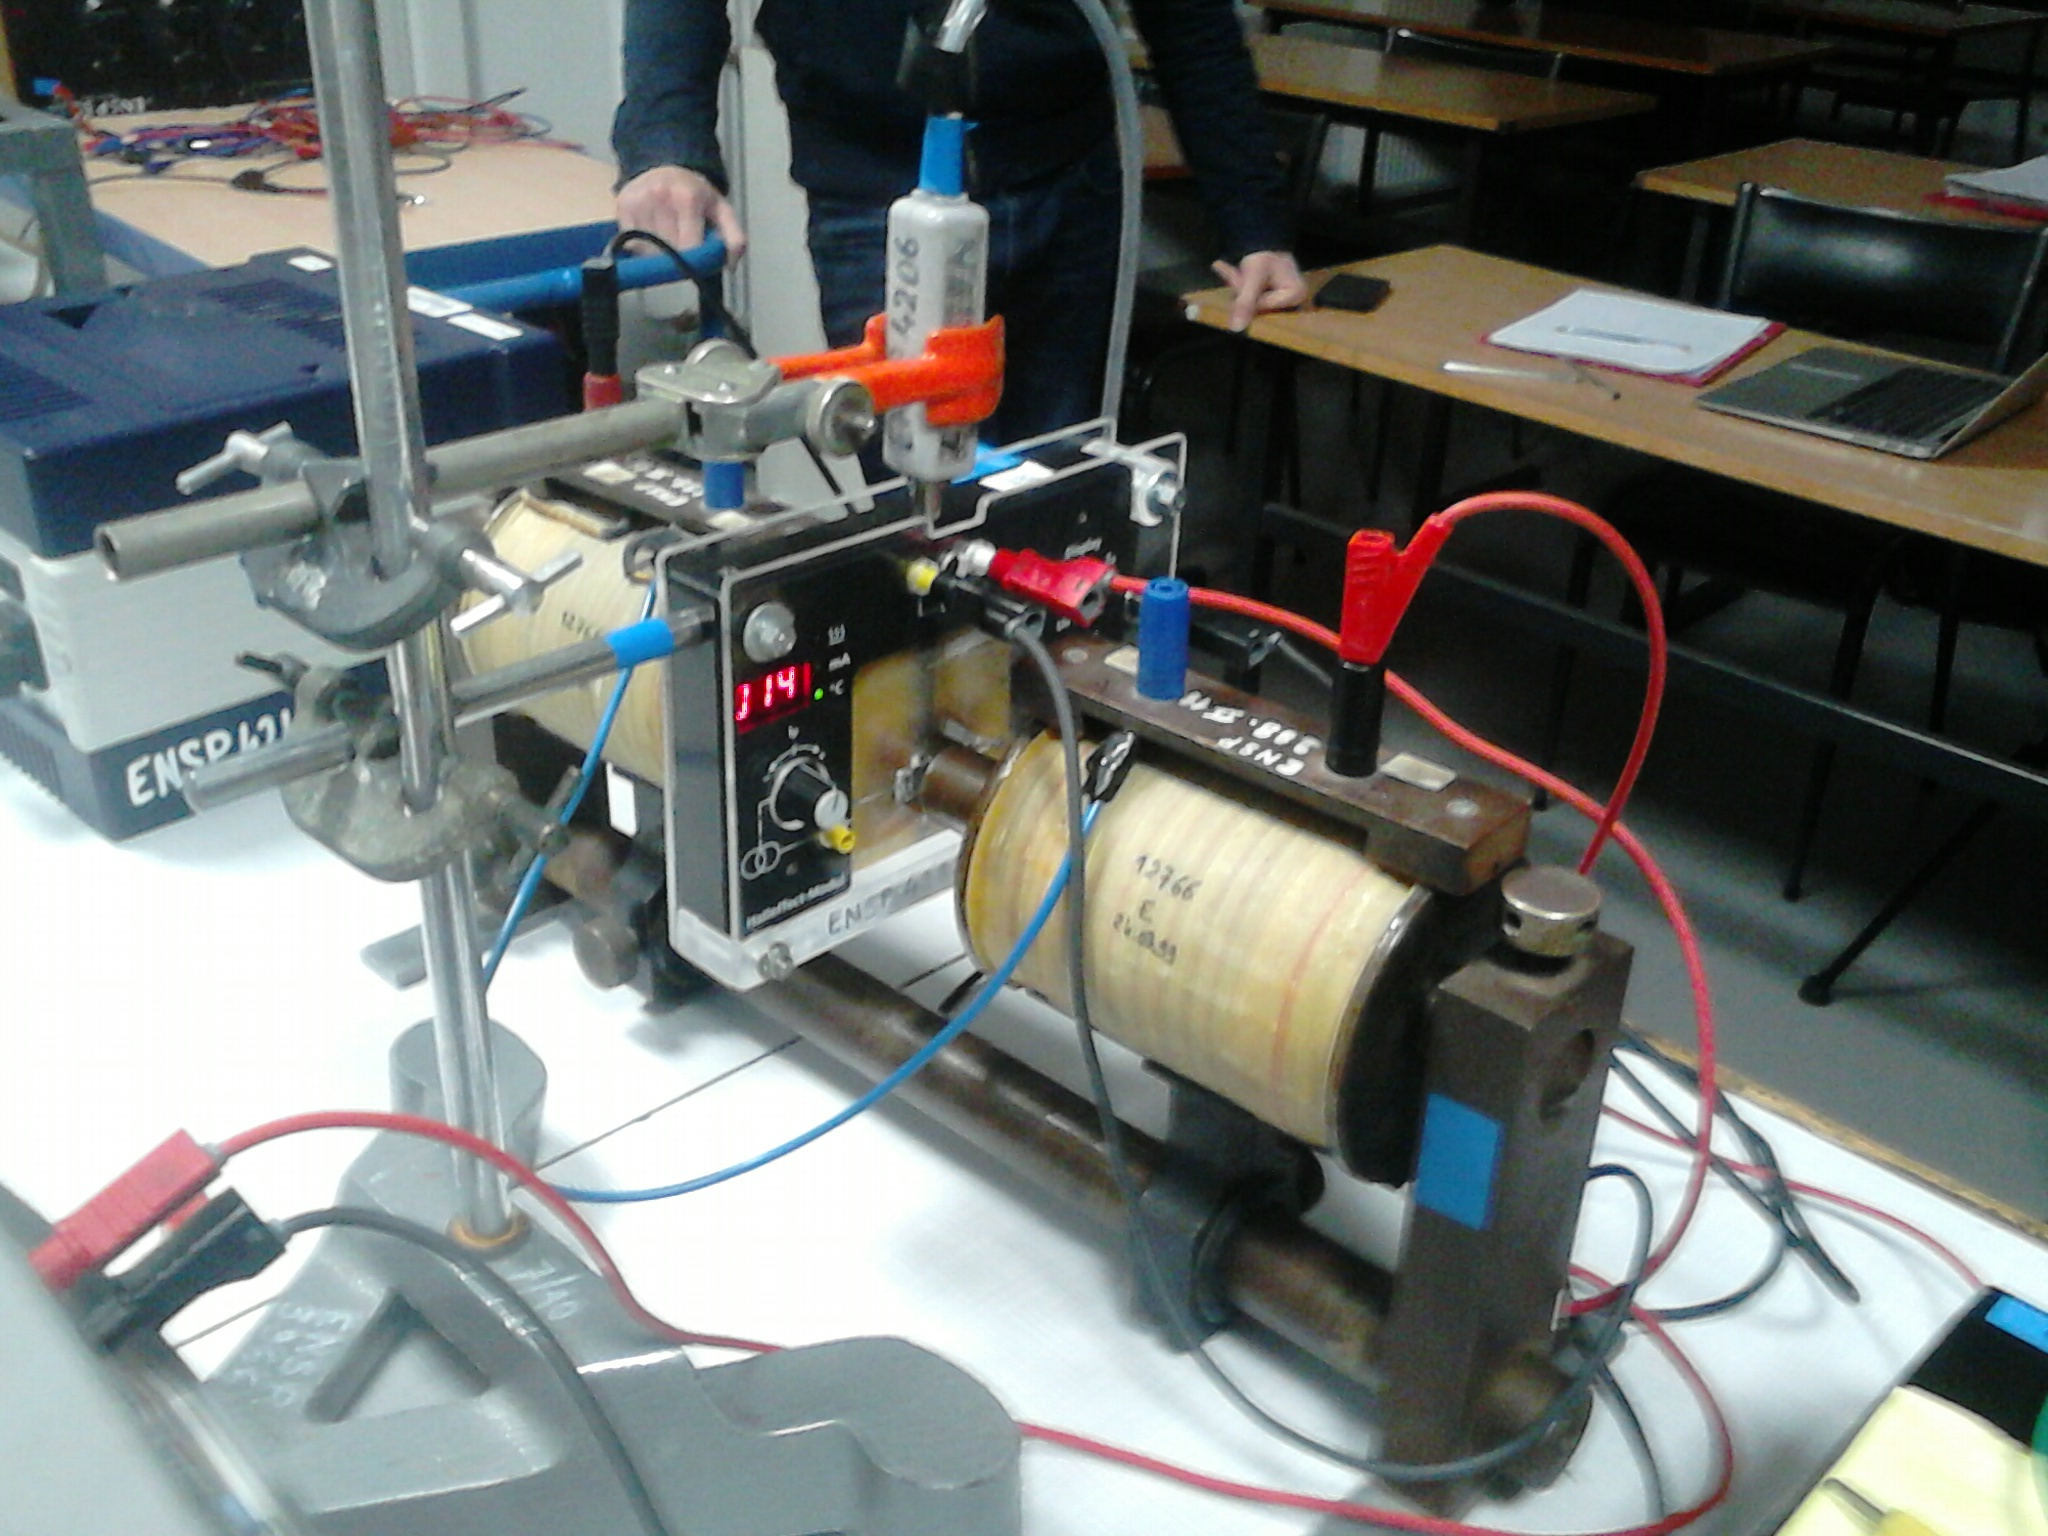
\includegraphics[width=10cm]{images-exp/Hall.jpg}}
	\caption{Expérience de l'effet Hall}
\end{figure}

Soit n la densité de porteurs, q leur charge (algébrique), et $\vec{v}$ leur vitesse moyenne définie par la densité de courant:

$\vec{j} = \frac{\displaystyle I}{\displaystyle ab}\vec{e}_x = nq\vec{v}$.

Chaque porteur est soumis à la force de Lorentz $\vec{F} = q\vec{v}\wedge \vec{B}$.

Cette force tend à dévier les porteurs qui s'accumulent sur la face latérale ( $\bot Oy$) du barreau : il se crée donc un champ électrique $\vec{E}_{H}$ parallèle à Oy. En régime permanent, les trajectoires des porteurs sont parallèles à Ox et les deux forces se compensent exactement :

$q \vec{v}\wedge\vec{B} + q\vec{E}_{H} = \vec{0}$, soit :
$\vec{E}_{H} = \frac{\displaystyle - I B}{\displaystyle a b n q}\vec{e}_x \wedge \vec{e}_z = \frac{\displaystyle I\,B}{\displaystyle a b n q}\vec{e}_y$.

D'où la tension de Hall :
$V_{H} = V_{C} - V_{D} = \frac{\displaystyle I B}{\displaystyle b nq}$;

On a ainsi accès à la fois au type de porteurs (signe de q) et à leur concentration.

L'expression simple précédente n'est valable que si un seul type de porteurs contribue à la conductivité, ce que nous avons supposé depuis le début.

On notera que plus la concentration des porteurs est élevée plus l'effet Hall est petit. L'effet Hall existe aussi dans les métaux mais y est souvent difficilement mesurable car n est trop élevée. Par contre dans les semiconducteurs, où n est plus faible, $V_{H}$ est facilement mesurable.


Application de l'effet Hall dans un semiconducteur : le teslamètre.
Réalisation de l'expérience

Mesurer $V_{C} - V_{D}$ avec un voltmètre. Comme il est difficile de placer les deux contacts C et D exactement l'un en face de l'autre, la d.d.p. $V_{C} - V_{D}$ comporte une partie de chute ohmique. Annuler celle-ci au préalable en l'absence de champ magnétique en agissant sur le potentiomètre de compensation.

Placer ensuite le barreau de germanium dans l'entrefer d'un électroaimant ( $\vec{B} \parallel Oz$). Ne laisser l'électroaimant branché que pendant les quelques secondes nécessaires à la mesure, sinon il chauffe et perturbe fortement la mesure. Mesurer le champ magnétique B et la différence de potentiel $V_{C} - V_{D}$ . Vérifier que $V_{H} \left( \vec{B} \right) = - V_{H} \left( { - \vec{B}}\right)$. On peut éventuellement montrer la proportionnalité de $V_{H}$ à $B$.

Vérifier que la tension de Hall s'inverse lorsqu'on passe d'un échantillon de type n à un échantillon de type p.
Déduire du signe de la tension de Hall la nature des porteurs libres, ainsi que leur concentration :
$ n = \frac{I B}{qbV_{H} }$.
Quelle est la concentration relative des impuretés dopantes par rapport aux atomes du cristal, sachant que chaque atome dopant fournit un porteur ?

En combinant les mesures d'effet Hall et de résistivité, déterminer la mobilité $\mu$ des porteurs. On pourra vérifier, à l'aide des figures fournies dans la notice

ccl : étude de certaines caractéristiques des matériaux (ptés optiques, élec\dots) permettent de retrouver des propriétésintrinsèque des matériaux (énergie de gap, densité de porteurs de charge)
\section{Effets capacitifs.}
\underline{Références :}
\begin{itemize}
	\item Quaranta
	\item Duffait
	\item Cours de Feynman (elecmag)
\end{itemize}
\subsection{Condensateur plan d'Aepinius}
Modifier $e$ (décroît) et vérifier la formule


\subsection{Capteur de surface}
Géométrie cylindrique, le niveau d'eau est relié à la capacité.

Voir plus haut
\subsection{Mesure de la capacité d'un câble coaxial}

\textit{Caractéristiques d'un câble coaxial}

La mesure des caractéristiques d'un tel câble peut se faire grâce à un appareil spécifique, le LCR-mètre. Son utilisation demande de bien comprendre les phénomènes en jeu et de prendre quelques précautions. Vous constaterez par l'expérience que tout écart à son utilisation optimale peut mener à des valeurs de L ou C tout à fait aberrantes. Les réglages spécifiés ci-après sont justifiés qualitativement et quantitativement en annexe.

\textit{Capacité linéique}

La mesure de la capacité s'effectue au LCR-mètre :
\begin{itemize}
	\item    En circuit ouvert (une extrémité du câble libre, l'autre reliée au LCR-mètre).
	\item    A la fréquence la plus basse permise et/ou à la fréquence de travail.
\end{itemize}

\textit{Inductance linéique}

La mesure d'inductance s'effectue au LCR-mètre :

\begin{itemize}
	\item    En court-circuit (relier l'âme et la gaine du câble à l’extrémité non branchée au LCR-mètre).
	\item    A la fréquence la plus basse permise et/ou à la fréquence de travail.
\end{itemize}

\textit{Impédance d'un câble coaxial}

[1P] Impédance caractéristique

On appelle impédance caractéristique du câble le rapport entre la tension et le courant d'une onde électrique progressive. Elle est donnée par :

\[ Z_C = \sqrt{\frac{L_0 }{C_0 }}\]

Déduire sa valeur des grandeurs mesurées précédemment (cette valeur n'est pas universelle ; par exemple, certains câbles utilisés pour la vidéo ont une impédance caractéristique de $75 \Omega$ alors que les câbles utilisés en TP on une impédance précisément de $50 \Omega$ adaptée aux impédances de sorties des générateurs).

Il est aussi possible d'effectuer une mesure directe de cette impédance caractéristique en envoyant une impulsion de très courte durée dans le câble étudiant la façon dont elle est réfléchie en fonction de l'impédance placée à l'autre extrêmité. Faite le montage de la figure ci-dessous et commencer par comprendre l'effet des différents boutons du générateur d'impulsions (ENSP4005) sur la forme du signal. Aboutir à des impulsions courtes ( $\approx 0,1  \mu s$) pour éviter d'avoir un recouvrement entre les impulsions incidente et réfléchie.

OndesIICableCoaxial.svg

Comparer l'impulsion incidente et l'impulsion réfléchie en fonction des différentes valeurs R du potentiomètre. En déduire la valeur de l'impédance caractéristique $Z_{C}$ du câble [le coefficient de réflexion, en tension, vaut ($R-Z_{C})/(R+Z_{C})$]. Comparer cette valeur à celle obtenue à partir des inductance et capacité linéiques mesurées plus haut. Mesurer également l'amplitude des impulsions en début de câble et en déduire l'atténuation sur la longueur des câbles.

Remarque : En extrémité de câble (où R est connectée), la tension résulte de la superposition de celles des ondes incidente et réfléchie. En conséquence, (i) il est possible d'obtenir plus précisément l'impédance caractéristique en mesurant d'abord la tension $U_{o}$ à l'extrémité lorsqu'elle est ouverte ( R infinie), puis en cherchant la valeur de R ( = $Z_{C}$) pour laquelle cette tension est divisée par deux ; (ii) une mesure de $Z_{C}$ encore plus précise (mais plus longue) peut être obtenue en étudiant la tension U à l'extrémité du câble en fonction de la résistance R (la loi $U_{o}/U = 1 + Z_{C}/R$, facile à retrouver, est alors utile). 

\section{Induction, auto-induction.}

\underline{Références :}
\begin{itemize}
	\item Quaranta
	\item Hprépa, Brébec
\end{itemize}

\subsection{Passage d'un aimant dans une bobine}
Expérience qualitative, loi de lenz
\subsection{Mesure d'une inductance}
Par étude fréquentielle,relier à $N$

Avec diag Bode ou réponse indicielle
\subsection{Mesure d'une inductance mutuelle}
Envoi tension triangulaire sur l'une, on obtient des créneaux sur l'autre.

Inductance mutuelle et coefficient de couplage

CircuitElecBobinesCouplees.svg

La proximité entre deux circuits inductifs fait apparaître un coefficient d'induction mutuelle M, qui dépend de la géométrie de l'ensemble. On a alors :
\[ v_2 = L_2 \frac{di_2 }{dt} + M\frac{di_1 }{dt}\]

Dans le cas où $i_{2}=0$ (circuit ouvert), on aura donc $v_{2} = j M \omega i_{1}$ en régime sinusoïdal ($ j^2\equiv -1$). On fera l'expérience avec 2 bobines Leybold accolées (voir figure ci-après).

CircuitElecBobinesCoupleesMontage.svg

En déduire le coefficient de couplage défini par $\theta = \frac{M}{\sqrt {L_1 L_2 } }$, en déterminant $L_{1}$ et $L_{2}$ avec un LCR-mètre.
Complément :

Fermer le circuit magnétique à l'aide d'un étrier Leybold (en fer doux) et déterminer à nouveau $\theta$ (justifier qualitativement la nouvelle valeur obtenue). Il y a cependant une difficulté : le comportement devient très non linéaire (pourquoi ?).

On peut aussi faire cette expérience avec les solénoïdes enroulés l'un autour de l'autre, avec ou sans le noyau de fer doux (attention, il aura ici un rôle un peu différent de l'étrier mentionné précédemment). 

ccl : Observer phénomènes d'induction : loi de modération, auto-induction et couplage

\section{Production et conversion d'énergie électrique.}
Intro sur les enjeux
\subsection{Etude d'une cellule photovoltaïque}
\begin{itemize}
\item Caractéristique courant-tension
\item Puissance nominale
\item Rendement
\end{itemize}

Voir plus haut
\subsection{Conversion Alternatif-alternatif : le transformateur}
\begin{itemize}
\item rendement nominal
\item estimation des pertes
\end{itemize}
Préambule

La modélisation du transformateur est donnée en annexe.

Pour le bilan énergétique, on utilisera un transformateur d'isolement 160 VA, 110 V/55 V, plutôt qu'un transformateur démontable, dont les fuites magnétiques sont plus importantes. À l'inverse, on utilisera un transformateur démontable pour l'étude du cycle d'hystérésis.

L'alimentation du primaire se fera avec un alternostat 220 V/ 110 V.

Précaution : un transformateur est limité indépendamment en tension et en courant. Pour un transformateur de puissance apparente 160 VA, de tension d'entrée 110 V et de sortie 55 V, l'entrée ne doit pas avoir une tension supérieure à 110 V et un courant supérieur à 160 VA / 110 V $\approx$ 1,5 A (même si elle est alimentée effectivement sous 10 V). De même, le courant secondaire ne doit pas dépasser 160 VA / 55 V$\approx$ 3 A (même si le secondaire est court-circuité).
[1P] Bilan énergétique dans un transformateur en utilisation normale (régime non linéaire)

Du fait de leur non-idéalité, il existe des sources de pertes dans le transformateur. La méthode des pertes séparées permet de mesurer séparément ces différentes pertes. C'est l'objet de l'étude qui suit.
BilanEnergetiqueTransformateur3.svg

En l'absence d'alimentation, évaluer les résistances du primaire et du secondaire à l'ohmmètre.

On se place dans des conditions réalistes de fonctionnement en envoyant une tension de 110 V au primaire (tension nominale), avec une charge $R_c$ au secondaire (un rhéostat).
En charge

Choisir $R_{c}$ pour que la puissance au primaire $W_{1}$ soit la plus grande possible en respectant les limitations en courant et tension du transformateur et du rhéostat. Mesurer la puissance $W_{2}$ dans la charge $R_{c}$. Mesurer les courants $i_{1}$ et $i_{2}$.
Secondaire ouvert

Ne pas changer la tension d'alimentation ( $V_{1} = Cste$) afin que le champ magnétique (et donc les pertes fer) conservent la même valeur que précédemment.

Dans cette configuration, il n'y a pas de courant qui passe dans le secondaire. Les pertes Joule sont donc très faibles. En revanche, on a une forte tension et les pertes magnétiques sont élevées.

Mesurer la puissance au primaire. Elle représente les pertes dans le fer $W_{\mbox{FER}}$ (pertes par hystérésis et par courants de Foucault) car les pertes cuivres sont négligeables (le vérifier à partir des valeurs des résistances des bobinages).

Annuler $V_1$ avant de passer à la suite !!!
Secondaire court-circuité

Court-circuiter le secondaire sur un ampèremètre, puis augmenter doucement $V_1$ jusqu'à ce que le courant au secondaire atteigne la valeur mesurée en charge. Lors de ce fonctionnement en court-circuit, la tension $V_1$ est faible, et donc les pertes magnétiques également. En revanche les pertes par effet Joule dans le cuivre sont celles que l'on avait pour le fonctionnement en charge (courants identiques).

Mesurer la puissance au primaire. Elle représente les pertes dans le cuivre $W_{\mbox{CU}}$.

Vérifier enfin que :
$W_{1} \approx W_2 + W_{\mbox{FER}} + W_{\mbox{CU}}$

Problème classique: si vous trouvez que l'ampèremètre indique un courant nul en permanence, c'est que son fusible est à changer.
[1P] Étude du cycle d'hystérésis du fer d'un transformateur

Journeaux, Travaux Pratiques de Physique, pour une description succincte de l'expérience.
Montage expérimental

On réalise le montage ci-dessous où :

    Transfo = Transformateur Leybold démontable,
    $n_{1 } = 500$ spires,
    $n_{2 } \le n_{1}$, pour des questions de sécurité,
    $R = 20 à 30 \Omega : RHEOSTAT et non boîte AOIP car I_{1} > 1 \textrm{A}$ !
    $C = 4 à 10 \,\mu\textrm{F}$,
   $ R' = boîte AOIP \times 10^{5}$.


MagnetismeMontageCycle.svg

Attention ! : pour des raisons de sécurité, le transformateur variable placé à l'entrée doit être un vrai transformateur, à enroulements primaires et secondaires séparés, pas un autotransformateur.
Explication

    en X: on mesure aux bornes de R la tension $V_{x} = RI$ où I est l'intensité dans le primaire, donc une grandeur proportionnelle à H dans le fer. Le coefficient de proportionnalité est facile à calculer en fonction de R, $n_{1}$ et de la longueur L du circuit magnétique. L'expérience montre que c'est bien elle qu'il faut prendre en compte dans le théorème d'Ampère, pas la longueur de la bobine du primaire.

    en Y: la tension totale de sortie est $v_{2} = d\Phi /dt=n_2 s dB/dt$, où $n_{2}$ est le nombre de spires du secondaire et s la surface de la section du fer (et non pas des bobines). On ne peut pas utiliser directement cette tension, il faut l'intégrer au moyen d'un circuit intégrateur constitué par une résistance R' et une capacité C.

MagnetismeMontageRCCycle.svg

À tout instant :
$ v_{2} = R'i + \int {i\over C} dt$.

Nous choisissons donc $R'$ et $ C$ de telle sorte que : $ R'i \gg \int (i/C) dt$ (tension aux bornes de $ C$ négligeable), ce qui pour un signal de pulsation fondamentale $\omega_0$ se traduit par $ R'C \gg 1/\omega_0$. On peut alors écrire $i \approx v_{2}/R'$ et en déduire que la tension aux bornes de $ C$ est :
$ V_{c} = {1\over C}\int \frac{v_2 }{R'} dt = {1\over R'C} \int v_{2} dt = - \frac{n_2 s}{R'C}\int dB = - \frac{n_2 s}{R'C} B$

On peut ainsi étalonner les axes X et Y de l'oscilloscope.

À partir du cycle obtenu à l'écran, on déterminera :
\begin{itemize}
	\item    le champ $B_S$ à saturation,
	\item    le champ rémanent $B_R$,
	\item    l'excitation magnétique coercitive $H_C$,
	\item    la susceptibilité $\chi_0$ (c'est un coefficient de réponse linéaire, en pratique on le mesure en utilisant une très petite excursion);
	\item    les pertes par hystérésis (aire du cycle) ; en déduire la puissance perdue par le transformateur.
\end{itemize}

Note importante : En prenant les nombres de spires proposés ci-dessus vous constatez que la saturation n'est pas atteinte. Pour l'avoir, diviser par 2 le nombre de spires du primaire (point milieu du bobinage). Pourquoi a-t-on cet effet ? Pourquoi le bobinage du secondaire n'a-t-il aucun effet sur la saturation[1]?

Les tôles de transformateur sont faites avec des aciers au silicium (voir HANDBOOK à "Transformer steels permeability") ; il est aussi possible de comparer les résultats obtenus aux valeurs données dans les livres pour des aciers "moyens" (voir par ex. Rocard, Électricité, chap. IV, ou Bertin Faroux Renault, Électromagnétisme 4).
Expérience complémentaire : pour montrer le rôle des courants de Foucault, prendre un strap court, l'enrouler une fois autour du fer comme s'il constituait une 3ème bobine et le fermer sur lui-même. L'effet sur le cycle d'hystérésis est spectaculaire. Débrancher très vite avant que ça fume ("habemus papam").
[2P] Transport de puissance par ligne à haute tension

Référence : Bruhat, Électricité, page 641.

On propose une expérience qualitative, qui illustre pourquoi EDF a tout intérêt à transporter le courant via des lignes à haute voire très haute tension.

Réaliser le montage ci-dessous : le rhéostat R modélise la résistance de la ligne de transport (entre la centrale et l'utilisateur final). Travailler à fréquence assez basse (à cause des transformateurs utilisés plus loin).

Htetension1.svg

Régler l'amplitude du signal BF pour avoir un son fort lorsque R=0, puis faire croître R jusqu'à ce que le son soit quasi inaudible. En utilisant deux transformateurs identiques, passer en ligne "haute tension" comme indiqué sur la figure ci-dessous. Interpréter en ramenant toutes les impédances sur la sortie de l'ampli de puissance (c.f. III Annexe).
Htetension2.svg

\subsection{Interêt de la conversion en haute tension}
bilan de puissance et pertes avec et sans transfos.

\section{Amplification de signaux.}

Cours élec

\subsection{Amplificateur opérationnel}
Montage amplificateur ou ampli inverseur

\begin{itemize}
\item Mesure du gain
\item Etude fréquentielle (pduit gain bande, diag Bode)
\item Limitations ( tension, courant sortie)
\end{itemize}

 Caractéristiques et branchement des amplificateurs opérationnels

 Généralités

On utilisera un AO classique 741 qui a des performances assez modestes. On dispose également d'amplis op. TL 071 (ou de son frère jumeau TL 081) plus performant mais d'emploi plus délicat. Des notices du fabricant sont jointes au matériel. Le tableau suivant compare les caractéristiques essentielles des amplis 741 et TL 071 à celles de l'ampli op. parfait.
Caractéristiques des différents AO
Branchement du circuit intégré

Broches :

    [--] entrées (+, -) et sortie,
    [--] +A, -A : alimentation de l'ampli op,
    [--] OF : deux entrées permettant la correction de la tension de décalage d'entrée (voir plus loin),
    [--] NC : non connectée.

L'ampli op. est alimenté par deux tensions continues appliquées entre +A et -A, symétriques autour d'un point milieu, relié ou non à la terre. C'est ce point milieu qui donne la tension de référence (indiquée par 0) dans les montages de l'ampli op. Noter que sur les plaquettes sur lesquelles sont installés les AO, ce point milieu n'est relié à rien (retourner la plaquette pour le constater) : c'est à vous d'en faire un potentiel de référence du circuit. Avant toute utilisation, vérifier l'état de l'ampli op. en utilisant l'un des testeurs.
Réglage du décalage (offset)

C'est une tension continue parasite interne à l'ampli op. Ramenée à l'entrée, elle est de quelques mV qui seront amplifiés au niveau de la sortie (M. VAUCHELLES - Travaux pratiques d'électronique, chap IX)

Pour permettre d'annuler l'offset, le constructeur a prévu deux broches (notées OF sur les schémas) entre lesquelles on branche un potentiomètre de $10 k\Omega$ dont le curseur est relié au -12 V. Les plaquettes sont prévues avec ce potentiomètre connecté (petit boîtier rectangulaire dont le réglage par tournevis est très démultiplié). Le schéma Fig. 3 indique une méthode de réglage. Elle est analogue aux montages amplificateurs décrits plus loin, où l'on aurait annulé la tension d'entrée. Ici l'amplification est 11. Ajuster le potentiomètre de façon à annuler approximativement la tension de sortie (à 0,01 V près). Ce potentiomètre de réglage ne figurera pas sur les schémas ultérieurs.

Réglage de l'offset

Nous conseillons fortement de réaliser toutes les manipulations (sauf contre-indication précise) avec un 741. En effet l'utilisation d'un TL071 conduit ici très souvent à des oscillations parasites dont il est difficile de se débarrasser. Ceci tient surtout au fait que l'on réalise les montages avec des fils longs.
Amplification en continu et en basse fréquence

Dans cette partie on se limite à $G < 100$ et $f < 1 kHz$ pour ne pas faire apparaître les limitations en fréquence de l'ampli-op. (cf III). On s'intéressera davantage dans cette partie aux limites des AO qu'à la vérification des lois de gain.
[1P] Amplification avec inversion
Montage inverseur
Ampli op. idéal

Le gain est $G = \frac{V_s}{V_e} = -\frac{R_2}{R_1}$ (à établir). Pour le choix des résistances : la sortie de l'ampli op. débite le courant $i=V_s/R_2$ qui ne doit pas dépasser $10 mA$ pour rester dans un régime linéaire. La tension de sortie ne pouvant dépasser $\pm 15 V$ , on prendra $ R_{2} > 1 k \Omega$ . Choisir $R_{1}$ pour avoir un gain assez faible. Il ne faut cependant pas prendre $ R_{2}$ trop grand car d'autres défauts commencent à apparaître : tension d'offset, capacités parasites, etc (cf Dattée p. 98). Injecter un signal sinusoïdal de faible fréquence et vérifier la loi du gain (amplitude et phase).
Ampli op. non idéal

Saturation en tension : faire croître la tension d'entrée, interpréter.

Limitation en courant : faire débiter l'ampli op. sur une faible résistance, branchée entre la sortie et la masse. En déduire le courant maximum qu'il peut débiter. Ce montage peut-il alimenter un haut-parleur ?
[1P] Amplification sans inversion
Montage non-inverseur

Gain $G = \frac{V_s}{V_e} = 1 + \frac{R_2}{R_1}$ (à vérifier). Choix des résistances : quelle est la résistance vue par la sortie de l'ampli op. (en tant que composant électronique)? Que devient la condition sur les résistances pour rester en régime linéaire ? Le principal intérêt de ce montage est sa très grande résistance d'entrée illustrée dans le paragraphe «suiveur de tension».
Le suiveur de tension
Montage suiveur

C'est un cas particulier de l'amplificateur sans inversion, il n'amplifie pas en tension, $V_{s} = V_{e}$, mais possède une très grande résistance d'entrée et une très faible résistance de sortie.

Le montage suiveur est très largement utilisé car il permet de mesurer ou de prélever une tension sans modifier le fonctionnement du circuit étudié. On donne ici un exemple, où l'on cherche à mesurer la charge portée par un condensateur.
[1P] Ampli op. idéal : Mesure de la charge portée par un condensateur

Charger un condensateur de l'ordre de $1 \textstyle \mu F$ (pour éviter que la charge ou la décharge soient trop violentes, mettre toujours une résistance de l'ordre de $1 k \Omega$ en série avec le condensateur). Mesurer ensuite la tension à ses bornes avec un voltmètre pour en déduire la charge contenue dans le condensateur. Que constatez-vous ?

On améliore le montage ci-dessus en insérant un montage suiveur (figure 7) utilisant un TL071. Constater que l'appareil ainsi réalisé permet cette fois de mesurer la tension aux bornes du condensateur sans le décharger. Quelle est la différence avec le voltmètre précédemment utilisé ? (M. KROB - Électronique expérimentale, chap IV (et II))
Voltmètre électrostatique
[2P] Ampli op. non idéal : courant de polarisation

En réalité il y a une variation de charge très lente due non pas à la résistance d'entrée du montage qui est très grande mais au courant de polarisation d'entrée de l'ampli op. $i_{+}$ (courant continu qui provient de l'entrée +). En effet, la tension varie linéairement avec le temps et non pas exponentiellement.


Pour évaluer le courant de polarisation sur le TL071, remplacer le condensateur par un autre de valeur 100 fois plus faible, puis vérifier que la courbe $ V_{s} = f(t)$ est une droite et calculer $i_{+}$.

Constater que le courant de polarisation est 1000 fois plus élevé sur le uA741 en remplaçant l'ampli op. du montage précédent.
L'amplificateur opérationnel en «haute fréquence»

Deux phénomènes se superposent de façon indépendante :

    le gain diminue avec la fréquence, et il y a rotation de phase de $V_{s}$ par rapport à $ V_{e}$ ;
    la vitesse de variation de la tension de sortie $dV_s/dt$ est limitée :  $dV_s/dt < S$ (vitesse de balayage = slew rate) ; cela entraîne une limitation du gain à haute fréquence.

[1P] Étude de la vitesse limite de balayage

La vitesse limite de balayage ($ S = 0,5 V/ \mu s$ pour le 741) ne dépend pas du gain. Pour la mettre en évidence, il faut la dissocier de la variation du gain avec la fréquence (paragraphe suivant) : choisir le montage amplificateur non-inverseur par exemple et un gain faible (1 à 10), et utiliser des signaux de grande amplitude. Injecter un signal sinusoïdal et vérifier qu'il se déforme lorsque $\omega V_{s} > S$ où $V_{s}$ est l'amplitude du signal de sortie. Montrer qu'on obtient progressivement un signal triangulaire lorsqu'on augmente l'amplitude ou la pulsation (ce qui permet de détecter l'effet de cette limitation non linéaire).
[1P] Variation du gain avec la fréquence
Rappels

Le diagramme de Bode représente la variation du gain et du déphasage avec la fréquence (les valeurs correspondent au 741 sur les figures suivantes).
Diagramme de Bode

La phase initiale est 0 ou $\pi$ selon qu'on considère l'amplification sans ou avec inversion. La fréquence de coupure $f_{c}$ est définie pour le gain linéaire par $G(f_{c}) = G(f=0)/\sqrt{2}$ (soit pour le gain en dB : $ G_{dB}(f=0) - G_{dB}(f_{c})= 3{dB}$). Au-delà de $f_{c}$, la pente est toujours réglée à $ -20~dB/décade$, soit un gain linéaire $G(f)$ proportionnel à $1/f$. Cette compensation est réalisée par un condensateur interne, pour éviter qu'un déphasage de $\pi$ à haute fréquence ne transforme la contre-réaction en réaction, rendant alors le système instable (critère de Nyquist). Il en résulte que le produit $GAIN \times BANDE PASSANTE$ est constant pour le montage non inverseur : $G(f=0) \times f_c = cste$. Pour le montage inverseur la loi devient :  $( 1 + |G(f=0)| ) \times f_c = cste$. Il vaut environ 1 MHz pour le 741.

Manipulation

On utilisant le montage amplificateur inverseur (ou non-inverseur) (voir Krob), tracer en fonction de la fréquence la variation du gain (en log-log). Mesurer également le déphasage, en particulier au voisinage de la fréquence de coupure. En faisant varier le gain statique du montage, on pourra vérifier la loi sur le produit gain-bande.

Dans un deuxième temps, considère le montage en boucle ouverte, à savoir sans retour de la sortie sur l'entrée. On enverra ici un petit signal d'entrée sinusoïdal afin d'éviter la limite de vitesse de balayage (vérifier que le signal de sortie est sinusoïdal). La mesure du gain en boucle ouverte étant difficile, on se limitera à deux ou trois valeurs du gain, entre $ G = 10$ et $G = 1 000$, en commençant par les hautes fréquences (gain faible), par exemple 100 kHz. Une bonne manière d'obtenir ces mesures est de partir de la pente obtenue en boucle fermée, et la remonter progressivement en diminuant la fréquence. Cette étude est rendue difficile à grand gain par les bruits électroniques comme l'offset de l'AO qui deviennent du même ordre que la tension de consigne imposée par le GBF. Il est courant qu'au voisinage de $ 0 dB$ ($G = 1$) la courbe de gain devienne un peu plus verticale que $ -20 dB/déc$ donc que la loi étudiée ici ne soit plus bien vérifiée. C'est parce que la compensation en fréquence n'est plus nécessaire au-delà de $ 0 dB$.


Montage AO en boucle ouverte


\subsection{Ampli en puissance : le push-pull}
\begin{itemize}
\item Mesure du gain en tension et en puissance
\item Distorsion harmonique : insérer dans le montage avec un AO pour résoudre le problème
\end{itemize}

Ces composants dont l'invention a été récompensée par un prix Nobel en 1956 se retrouvent dans de nombreuses situations : amplification de puissance (le Push-Pull), stabilisation de tension (TP conversion de puissance électrique en série III) ou encore interrupteur (à la base des portes logiques). Les montages concernés comportent notamment Production et conversion d'énergie électrique et Amplification de signaux.
\begin{figure}
	\centerline{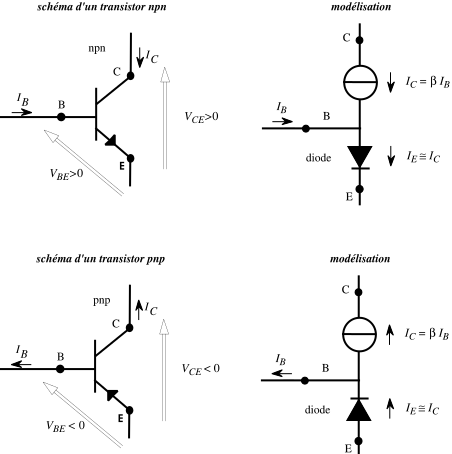
\includegraphics[width=10cm]{images-exp/schema_transistor.png}}
	\caption{Schéma transistor}
\end{figure}

\textit{Transistor npn et pnp.} B = base, C = collecteur, E = Émetteur. Le gain en courant $\beta$ est de l’ordre de 100. La flèche noire sur l’émetteur indique le sens $\emph{réel}$ du courant dans l’émetteur. Pour passer du npn au pnp, changer le signe de toutes les tensions et inverser le sens des courants.


Dans la suite on travaillera uniquement avec des transistors de puissance avec leur radiateur :

    npn : BD 439 (ou TIP 29)
    pnp : BD 440 (ou TIP 30)

Vérifier à chaque fois qu'ils sont en bon état en utilisant un testeur de transistor : celui-ci mesure $\beta$.

NOTE : Si dans les expériences qui suivent, le signal de sortie contient une composante de haute fréquence (plusieurs MHz) dont l'amplitude peut valoir 10 mV à plusieurs volts (le signal basse fréquence attendu semble «empâté»), c'est que l'amplificateur présente une instabilité. On indique dans la suite des précautions à prendre pour éviter ce phénomène

\begin{figure}
	\centerline{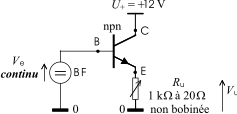
\includegraphics[width=10cm]{images-exp/Transistor_continu.png}}
	\caption{Etude en continu}
\end{figure}

\textit{Étude en alternatif}

\begin{figure}
	\centerline{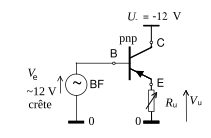
\includegraphics[width=10cm]{images-exp/Transistor_alternatif.png}}
	\caption{Etude en alternatif}
\end{figure}

Remplacer le signal continu sur la base du transistor par un signal purement sinusoïdal. Régler l'amplitude du signal à la limite de l'écrêtage de la partie positive de la tension de sortie (l'écrêtage correspond à une amplitude de environ 12V, mais les GBFs délivrant pour la plupart une amplitude maximale de 10V, il suffira de régler cette dernière sur 10V). Observer le signal d'entrée et le signal de sortie en même temps à l'oscilloscope. Expliquer le phénomène.


Remarque : on alimentant le transistor avec un alimentation continue de 5V (ou une valeur intermédiaire inférieure à 10V), on pourra observer facilement l'écrêtage.
[1P] Étude avec un transistor pnp
Transistor pnp en régime sinusoïdal.


En gardant le même signal sinusoïdal, remplacer le transistor npn par un transistor pnp, et l'alimentation $U_{+}$ par une alimentation $U_{-} = -12V$ (ou de -5V pour observer l'écrêtage). Observer.

En conclusion le suiveur à transistor npn permet de transmettre la puissance pendant l'alternance positive et le suiveur à transistor pnp pendant l'alternance négative. On utilise cette propriété dans l'expérience qui suit. 

\textit{Amplificateur push-pull}

Réaliser le montage ci-dessous, où les émetteurs des deux transistors sont connectés entre eux.
\begin{figure}
	\centerline{\includegraphics[width=10cm]{images-exp/Transistor_pushpull.png}}
	\caption{Montage push-pull}
\end{figure}

Comprendre son fonctionnement. On pourra notamment illustrer le rôle de chaque transistor en déconnectant sa base.

Comme précédemment, régler $V_{e}$ à la limite de l'écrêtage (avec une alimentation symétrique -5V/0/+5V) ou, à défaut, à la tension maximum du GBF.

Remarquer la «distorsion de croisement»[6].

D'où vient le nom de «push-pull»?


[1P] Estimation de la résistance de sortie de l'amplificateur push-pull

Afin d'évaluer l'impédance de sortie du montage push-pull, il convient de tracer la caractéristique $V_u=f(I_u)$ où $V_u$ est la tension de sortie du montage et $I_u$ le courant de sortie. En effet, dans le cas idéal ($Z_s \approx 0$), on a $V_u=V_e$ (sans tenir compte des décalages de 0.6V au niveau des jonctions), et ce indépendamment de la charge de sortie. Dans le cas réel, on a $V_u=V_e-Z_s\cdot I_u$, où $Z_s$ est l'impédance de sortie. Ainsi, en faisant varier la charge $R_u$, on fait varier le courant de sortie $I_u$ ainsi que $V_u$. On reconstruit la courbe $V_u=f(I_u)$, dont la pente donne accès à l'impédance $Z_s$. En pratique, les composants étant non linéaires, on n'obtient pas une droite, mais les valeurs autour d'un point de la caractéristique permettent de définir une impédance de sortie locale (Cf. cours d'électronique).

Manipulation : On modifie le courant débité $I_u$ en variant $R_u$. Mesurer $V_u$ pour quelques valeurs de $R_u$ (de $1k\Omega$ à $20\Omega$). Faire un tableau avec $R_u$, $V_u$ et $I_u=\frac{V_u}{R_u}$. Représenter la courbe $V_u=f(I_u)$ . Cette courbe n'est pas une droite mais déduire de ses variations une estimation de la résistance de sortie en signaux alternatifs de grande amplitude (dans le modèle du générateur de Thévenin).


Dans la suite, choisir une valeur fixe de $R_{u}$ qui corresponde à une puissance importante en régime permanent, sans cependant poser de problème d'échauffement ni de courant excessif : $R_{u}=20 \Omega$ devrait convenir[7].
[1P] Détermination de la puissance reçue par la charge utile

La charge étant une résistance, il n'est pas nécessaire d'utiliser un wattmètre (pas de $\cos \phi$ notable dans un résistance).

Placer un voltmètre alternatif RMS aux bornes de $R_{u}$ et appliquer la formule $ P_{u} = \frac{V^2_{u,efficace}}{R_{u}}$.
[1P] Détermination de la puissance fournie par les alimentations continues

Placer successivement un ampèremètre en mode continu en série avec chaque alimentation. Pourquoi utiliser un ampèremètre continu et non pas alternatif ?

On mesure alors $P_{alim} = \langle{U_+I_+ + U_-I_-}\rangle = U_+ \langle{I_+}\rangle + U_-\langle{I_-}\rangle$.

Déduire de ces deux mesures le rendement $\eta$ de l'amplificateur. Un calcul théorique conduit à $\eta \simeq \frac{\pi}{4} \frac{V_{s{cr\hat{e}te}}}{U_+}$, qui vaut environ $79\%$ si $V_{s,\mathrm{cr\hat{e}te}} \approx U_+$ i.e. le signal de sortie est à la limite de l'écrêtage.
[1P] Détermination de la puissance fournie par le générateur sinusoïdal

La charge vue par ce générateur n'est pas a priori modélisable par une simple résistance. Il faut donc utiliser un wattmètre (très sensible) pour effectuer cette mesure. En déduire le gain en puissance de l'amplificateur
[2P] Application pratique

Remplacer la résistance $R_u$ par un haut parleur et comparer au son obtenu sans l'amplificateur de puissance. 

\section{Mise en forme, transport et détection de l'information.}
\subsection{Modulation d'un signal en fréquence}

Références :

Duffait - Expériences d'électronique (chap.3 et chap.9)

Quaranta - Dictionnaire de physique expérimentale : électronique (tome III) (articles "démodulation" et "modulation")

Neffati - Traitement du signal analogique

Guillien - Électronique (tome 2)
[1P] Introduction

Lors d'une modulation en fréquence, l'onde électromagnétique porteuse voit sa pulsation $\omega_0=2\pi f_0$ modulée de $\omega _{0} - \Delta \omega$ à $\omega_{0}+\Delta \omega$ par un signal de basse fréquence de pulsation $\Omega =2\pi F$ :
\[ \omega = \omega _{0} + \Delta \omega \cdot \cos \Omega t = \frac{d\Phi }{dt}\]

où $\Phi$ est la phase du signal, donc $\Phi = \omega _{0}t + \frac{\Delta \omega }{\Omega } \cdot \sin\Omega t$ . L'excursion en pulsation $\Delta \omega$ est en général proportionnelle à l'amplitude du signal basse fréquence et dépend des caractéristiques du modulateur de fréquence. L'équation de l'amplitude de la porteuse est donc :
\[ v = a \cos\left(\omega _{0}t +\frac{\Delta \omega }{\Omega }\cdot \sin\Omega t\right)\]

Dans le cas d'une modulation en fréquence, l'indice de modulation est défini par :
\[ \beta = \frac{\Delta \omega}{\omega_0}\]
[1P] Réalisation sur un GBF

Les deux types de GBF disponibles à Montrouge permettent de réaliser une modulation de fréquence, mais avec quelques différences. Il est conseillé de s'entraîner sur les deux modèles.
METRIX GX320

Choisir la fonction MODUL, et la source EXT. Ici on ne choisit pas la fréquence centrale, mais directement les fréquences de départ et d'arrivée (on change en restant appuyé sur FREQ). Le signal modulant est envoyé sur l'entrée VCG IN : amplitude 20 Vpp pour explorer toute la gamme de fréquences choisie précédemment, fréquence < 15 kHz.

Correspondance signal modulant/fréquence de sortie du GBF : $+ 10 \ \rm V \to \mathtt{Freq_{End}}$, $- 10 \ \rm V \to \mathtt{Freq_{Start}}$,$ 0 \ \rm V \to (\mathtt{Freq_{Start} + Freq_{End}})/2$
KEYSIGHT 33500B, AGILENT 33220A et équivalents

On décrit principalement la démarche pour le KEYSIGHT 33500B (le plus moderne et le plus agréable à utiliser), mais c'est la même chose pour les autres, à de légères différences de nom près.

Utiliser l'entrée arrière MODULATION IN. Dans Parameters, choisir la fréquence centrale $f_0$ et l'amplitude de sortie $V $.

Important : avec ces GBF, il faut, pour une voie donnée, choisir CH output > Output Load > Set to High Z afin que la tension affichée correspond à la tension réellement générée.

Pour la modulation de fréquence : cliquer sur Modulate, choisir Type > FM et Source > External.

L'excursion en fréquence est contrôlée par le paramètre Freq Dev, qui donne l'excursion pour une entrée de $ + 5  \rm V$ . Autrement dit, pour un signal modulant $u_m(t)$ sur l'entrée MODULATION IN, la fréquence instantanée du signal de sortie sera :
$f = f_0 + \frac{\mathtt{Freq Dev}}{5 \ \rm V} \, u_m(t) \equiv f_0 + g u_m(t)$

où on définit $g$ , "gain" de l'oscillateur contrôlé en tension.

Manipulation : Réaliser une modulation de fréquence avec différents signaux modulants (sinusoïde, carré) et observer le signal de sortie à l'oscilloscope.
[2P] Spectre d'un signal modulé en fréquence

Contrairement à la modulation d'amplitude, le spectre d'un signal modulé en fréquence contient une infinité de raies :
\[ v = a \sum_{n=-\infty}^{+\infty} J_n(\beta) \cos\left(\omega_0 + n\Omega\right) t\]

avec $\textstyle J_n(\beta)$ la fonction de Bessel d'ordre $ n$. La règle de Carson énonce que 98\% de l’énergie du signal modulé en fréquence par une sinusoïde se situe dans l’intervalle :
$\omega _{0} - (\Delta \omega + \Omega) \le \omega_0 \le \omega_0 + (\Delta \omega + \Omega)$

On se propose de vérifier cette règle.

Manipulation :

Utiliser un GBF modulable en fréquence réglé sur une porteuse de fréquence $f_{0}$ de l'ordre de 10 kHz. Le signal basse fréquence ($F$) sinusoïdal est délivré par un autre GBF et injecté sur l'entrée modulation du premier.

    Mesurer l'excursion en fréquence (et l'indice de modulation $\beta$ ). Méthode possible : sur l'écran de l'oscilloscope le signal modulé en fréquence forme une sinusoïde dont la période varie de $T_{min}$ à $T_{max}$. À l'aide du mode persistant, en déduire $f_{min}$ et $f_{max}$, puis $\Delta f=\Delta\omega/2\pi$.

    Analyser ensuite le spectre du signal modulé en fréquence avec l'oscilloscope numérique et vérifier approximativement la règle de Carson grâce à l'échelle verticale de l'oscilloscope. Pour cela, relever la hauteur $A_i$ de tous les pics observables en dBV, et convertir en tension efficace au carré (pourquoi s'intéresse-t-on au carré ?) :

\[ V_{eff,i}^2 = 10^{A_i/10} \ \rm V\]

Tronquer ensuite la somme à un indice i et repérer la fréquence $f_i$ pour laquelle le rapport de la somme tronquée avec la somme totale vaut 0,98. Vérifier alors la règle de Carson.

Exemples de cas que l'on peut étudier :
Tab1.svg

    Faire varier l'indice de modulation. Lorsque $\beta$ augmente, on constate que le spectre s'élargit, en accord avec la règle de Carson.
        Pour $\beta = 2,4$ la raie associée à la porteuse disparaît (mathématiquement, $J_0(2,4) = 0$) ;
        Pour $\beta = 3,8$ les deux premières raies latérales disparaisses (mathématiquement, $J_1(3,8) = 0$) ;

    Choisir à présent un signal triangle, puis carré et observer à nouveau la bande de Carson.


Quelques remarques :

L'émission radio FM (100 MHz) : celle-ci est obtenue en modifiant les caractéristiques d'un circuit oscillant par action du signal BF sur une capacité variable (diode varicap) ou sur une self variable (noyau de ferrite saturé); en pratique l'excursion en fréquence est très faible, ce qui la rend inobservable à l'oscilloscope. Ceci nous semble difficilement réalisable dans le cadre de l'agrégation.

Les générateurs de fonctions actuels (wobbulateurs) : ils fonctionnent sur un principe totalement différent :

    un générateur à relaxation produit des signaux triangulaires d'amplitude bien constante mais de fréquence variable.
    ces signaux sont envoyés dans un circuit non linéaire qui les transforme en sinusoïdes.

\subsection{Transport (câble) coaxial}

Différents aspects de la propagation d'un signal dans un câble coaxial ont déjà été étudiés dans le TP Ondes II. Par exemple, l'étude de la déformation d'un pulse se propageant dans un câble coaxial, la mesure de l'impédance caractéristique, de la vitesse de propagation... peuvent avoir leur place dans un montage ayant pour thème la transmission d'un signal. Nous proposons ici la mesure du coefficient d'atténuation d'un câble coaxial en fonction de sa longueur et de la fréquence du signal.

On peut envisager plusieurs méthodes :

    envoyer un pulse dans le câble en extrémité ouverte, comparer l'amplitude du pulse d'entrée et du pulse réfléchi (attention, la distance parcourue est $2 \times L$), cf. TP Ondes II ;
    envoyer un signal sinusoïdal de fréquence supérieure à 10 MHz (sinon l'atténuation est trop faible pour être précisément mesurable). L'autre extrémité du câble est connectée à un oscilloscope dont l'entrée commutable est accordée sur $50 \Omega$ (par exemple l'oscilloscope TDS 3014)[3]. Les mesures de tensions sont effectuées à l'oscilloscope car la bande passante des multimètres est généralement inférieure à 400 kHz.

Évaluer les pertes linéiques en utilisant des câbles de différentes longueurs. L'unité usuelle d'expression des pertes est le dB/100m.

Comment varient ces pertes avec la fréquence du signal ? 

\subsection{Démodulation : boucle à verrouillage de phase}
=> à bien expliquer

ou modulation AM et démodulation

Références :

Duffait - Expériences d'électronique (chap.9)

J. Esquieu - BUP 772, Transmissions numériques

P. Clerc - BUP 868 (2), Système dynamique et plan de phase : étude d'une PLL

Manneville et Esquieu - Électronique : systèmes bouclés linéaires, de communication et de filtrage (parties "systèmes bouclés linéaires", chap. 3.3 et "systèmes de communication")


La boucle à verrouillage de phase (PLL : Phase-Locked Loop) est un système asservi, couramment utilisé pour la démodulation de fréquence aussi bien en analogique qu'en numérique. Elle peut donc avoir sa place dans les montages "Mise en forme, transport et détection de l'information" et "Systèmes bouclés".

En guise d'illustration, on considèrera le dispositif suivant :
Montage pour la boucle à verrouillage de phase
\begin{figure}
	\centerline{\includegraphics[width=10cm]{images-exp/PLL.png}}
	\caption{Boucle à verouillage de phase}
\end{figure}

    GBF2 fournit une tension sinusoïdale de fréquence $f_{2 }$ qui peut être modulée sur son entrée VCF (Voltage Controlled Frequency) par GBF1. Dans la suite, on commence par étudier la boucle sans parler de modulation/démodulation, donc ne pas connecter GBF1.

Le reste du dispositif constitue la boucle à proprement parler :

    le comparateur de phase est ici un multiplieur analogique, qui réalise l'opération $u_m = k_m u_2 u_3$ , où $k_m \simeq 0,1 \ V^{-1}$ est le gain du multiplieur.
    le filtre passe-bas (ici un RC) élimine les composantes à haute fréquence de $u_m$ , il a pour fréquence de coupure $ f_F = \frac{1}{2 \pi RC}$ .
    l'oscillateur commandé en tension est ici GBF3, dont la fréquence instantanée de sortie est modulée autour de la fréquence centrale $f_3^0$ par la tension de sortie du filtre :

$f_3 \equiv \frac{1}{2 \pi} \frac{d \Phi_3}{dt} = f_3^0 + g u_F(t)$

    on place enfin un suiveur de tension[1] entre le filtre et l'entrée "modulation" du GBF3, car son impédance d'entrée n'est pas forcément grande devant R (la notice indique $5 k \Omega$ pour les KEYSIGHT 33500B). 

On dit que la boucle est verrouillée lorsque $f_3 = f_2$ . La plage de verrouillage est l’intervalle $\Delta f_v$ de fréquences à l'intérieur de laquelle on peut faire varier $f_2$ , la boucle restant verrouillée (la boucle "suit" les variations de $f_2$ ). Partant désormais de la boucle dans un état "non verrouillé", la plage de capture $\Delta f_c$ est l’intervalle de fréquences d’entrée pour lesquelles GBF3 est capable de se synchroniser sur GBF2. On s'attend logiquement à $\Delta f_c < \Delta f_v$ .

Matériel :

Le choix des différents composants est ici très important ; il faut notamment un gain g du GBF3 suffisamment important. On conseille ainsi d'utiliser les GBF les plus modernes (KEYSIGHT 33500B), au moins pour GBF3. Relire si nécessaire la discussion sur la modulation de fréquence avec ces GBF dans la section "Modulation de fréquence (FM)". Pour rappel, on a la relation importante $ g = Freq Dev/5  V$ .

Il est aussi possible d'utiliser de vieux GBF (GX 245), qui ont un gain g fixe et important, mais sont plus délicats à manier. On règle la fréquence centrale $f_3^0$ puis on active SWEEP EXT et l'entrée à utiliser est VCF IN.

Dans tous les cas, les Metrix GX320 (GBF bleus) sont très fortement déconseillés pour être GBF2 ou GBF3.


On pourra prendre comme valeurs typiques : $R = 10  k \Omega$ , $ f_2 \simeq f_3^0 = 10 kHz$ .


[1P] \textit{Principe de fonctionnement}

L'objectif est d'asservir la fréquence $f_3$ à $f_2$ . Si la fréquence de GBF3 varie, l'ensemble multiplieur-filtre fournit un signal qui ramène cette fréquence à sa valeur initiale. Et inversement si la fréquence fournie par GBF2 varie, la boucle d’asservissement permet à GBF3 de fournir un signal exactement à la nouvelle fréquence $f_2$ .

Le fonctionnement de la PLL est plutôt compliqué[2], mais l'important est de comprendre le mécanisme une fois la boucle verrouillée. Plaçons-nous donc dans ce cas : $f_3 = f_2$ . Alors $u_2(t)=V_{2} \cos(\omega_2 t)$ et $u_3(t)=V_{3} \cos(\omega_2 t + \phi)$ sont les tensions données par GBF2 et GBF3. La sortie du multiplieur fournit la tension :
\[ u_m(t) =k_m V_{2} \cos (\omega_2 t)\cdot V_{3} \cos (\omega_2 t + \phi) =\frac{1}{2}k_m V_{2} V_{3} \left[ \cos(\phi) + \cos( 2 \omega_2 t +\phi) \right]\]

Le filtre passe-bas est choisi de façon à ce que $f_F \ll f_2$ , il ne garde donc que la composante continue :
\[ u_F(t) = \frac{1}{2}k_m V_{2} V_{3} \cos(\phi)\]

D'où la fréquence de sortie de GBF3,
\[ f_3 = f_3^0 + g u_F(t) = f_3^0 + \frac{1}{2} g k_m V_{2} V_{3} \cos(\phi)\]

qui doit être égale à $f_2$ . Les limites $\cos(\phi) = \pm 1$ fixent ainsi la plage de verrouillage de la boucle, la fréquence centrale $f_3^0$ étant fixée initialement par l’utilisateur  :
\[ f_2^{min} = f_3^0 - \frac{1}{2} g k_m V_{2} V_{3} , f_2^{max} = f_3^0 +\frac{1}{2} g k_m V_{2} V_{3}\]

d'où
\[\Delta f_v = f_2^{max} - f_2^{min} =g k_m V_{2} V_{3}\]

Concernant la plage de capture, on peut proposer l'argument simple suivant : la boucle va accrocher si la composante basse fréquence de $u_m(t)$ est dans la bande-passante du filtre. Or dans le cas d'une boucle non verrouillée, cette composante est à la fréquence $f_2 - f_3^0$ . On s'attend donc à $\Delta f_c \sim f_F$ , mais on peut citer le résultat valable pour $\Delta f_v \gg f_F$ (cf. Duffait, Expériences d'électronique p235) :
\[ \Delta f_c = \sqrt{2 \cdot \Delta f_v \cdot f_F}\]

[1P] \textit{Étude de la boucle de verrouillage}

Afin d'étudier uniquement le système bouclé "PLL", ne pas connecter GBF1 pour le moment.

Il y a trois signaux à visualiser dans cette étude : les deux sorties des GBF 2 et 3 ainsi que la tension de sortie du filtre $u_F$. Pour faire toutes les observations qui suivent de façon simple, on pourra utiliser les 2 oscilloscopes de la façon suivante:

    Oscillo 1: Brancher sur CH1 la sortie $u_2(t)$ du GBF2, et sur CH2 la sortie $u_3(t)$ du GBF 3 ;
    Oscillo 2: Visualiser la sortie du filtre ( $u_F$).

    [1P] \textit{Premières manipulations}

    Fixer les fréquences de GBF2 ( $f_2$) et de GBF3 ( $f_3^0$) à deux valeurs très voisines. Visualiser les sorties des GBF avec K ouvert : la synchronisation des deux est impossible.

Fermer K : les deux signaux sont maintenant à la même fréquence. Si ce n'est pas le cas, approcher $f_2$ de $f_3^0$ ou agrandir la plage de capture en agissant par exemple sur les amplitudes $V_{2}$ et $V_{3}$.

Mettre en évidence l'asservissement et notamment les caractéristiques suivantes :

    faire varier $f_2$ : constater que $f_3$ suit $f_2$ ;
    corrélativement, $u_2$ et $u_3$ sont déphasées entre 0 et $\pi$, avec comme cas particulier $\phi =\pi/2$ quand $f_2 = f_{3}^0$ ;
    noter l'évolution de $u_F$ (tension de sortie du filtre) avec le déphasage ;
    montrer que le décrochage de l'asservissement a lieu quand le déphasage $\phi$ arrive aux valeurs extrêmes 0 et $\pi$ (plage de verrouillage) ;
    vérifier que la plage de verrouillage de l'asservissement est plus large que la plage de capture ;
    jouer sur les paramètres $V_2$ , $V_3$ (amplitudes des GBF) et $g$ (en modifiant Freq Dev), observer les variations des plages ;
    facultatif : modifier R ou C ; en vertu des formules donnant $\Delta f_c$ et $\Delta f_v$ , la plage de capture est modifiée mais pas celle de verrouillage.

    [2P] \textit{Observation en wobbulation}

Une manière élégante et didactique d'observer les plages de capture et de verrouillage est de réaliser un balayage automatique en fréquence de $f_2$ (wobbulation). Si GBF2 est un KEYSIGHT 33500B, une bonne solution est de choisir sur la voie 1 Modulate > Source > Channel 2. Sur la deuxième voie de GBF2, on fabrique le signal wobbulant comme une rampe d'amplitude 10 Vpp, fréquence de quelques dizaines de mHz et de Symmetry 50\%. Avec ces paramètres, le choix de Freq Dev sur la voie 1 détermine l'excursion en fréquence de $f_2$.

    Sur l'Oscillo 2, observer en X le signal de la voie 2 de GBF2 (ou bien la rampe de wobbulation que l'on peut obtenir directement sur d'autres GBF), et en Y la tension de sortie du filtre. En mettant de la persistance, observer les plages de verrouillage et de capture. Regarder en parallèle l'évolution du déphasage $\phi$ entre les deux signaux sur l'Oscillo 1.

    Vérifier les différentes observations précédentes (dépendance en les paramètres notamment) dans ce mode de visualisation.

    [1P] \textit{Manipulations quantitatives}

Dans le cadre d'un montage, on peut proposer quelques manipulations quantitatives autour de la PLL :

    plage de verrouillage $\Delta f_v$ en fonction de $g$ ou de $V_3$  ;
    plage de capture (moins conseillé que l'étude de la plage de verrouillage car relation moins claire donnant $\Delta f_c$ ) en fonction de $\Delta f_v$ ou $f_F$  ;
    relation entre $u_F$ et $ \phi$ . À noter que ce déphasage s'observe très joliment en passant en mode XY sur l'Oscillo 1.

Remarques et conseils

    Lorsqu'on parle de plage de verrouillage ou de capture, il faut regarder les limites de $f_2$ pour  $f_3^0$ fixée : étant donnée une PLL, on varie le signal d'entrée pour trouver les caractéristiques de cette boucle.
    Pour déterminer une plage, il faut aller doucement. Il faut notamment, lorsqu'on approche de $\phi = 0$ ou $\pi$ , faire des pas de plus en plus petits en fréquence.
    Si on oublie de mettre le suiveur en tension, la plage de verrouillage est réduite et les relations ci-dessus doivent être modifiées pour tenir compte de l'impédance d'entrée de l'entrée Modulation de GBF3.
    Pour être quantitatif, ne pas hésiter à re-mesurer le gain du multiplieur $k_m$ .

    [1P] \textit{Application à la démodulation de fréquence}

La tension de sortie du filtre est proportionnelle à la différence des fréquences $f_2$ (imposée par GBF2) et $f_{3}^0$ (que devrait fournir GBF3 sans l'asservissement), puisque par définition de la modulation de fréquence de GBF3,
\[ u_F(t) = \frac{f_3 - f_3^0}{g} = \frac{f_2 - f_3^0}{g}\]

si la boucle est verrouillée. On réalise ainsi une transformation fréquence-tension, donc une démodulation de fréquence !

Désormais, $f_2(t) = f_p + \Delta f \cos(2 \pi f_1 t)$ (modulation de fréquence). Si la fréquence ne varie pas trop vite, la boucle peut rester verrouillée à chaque instant. Alors la PLL réalise une démodulation de fréquence via (on prend $f_p = f_3^0$ pour simplifier) :
\[ u_F(t) =\frac{\Delta f}{g} \cos(2 \pi f_1 t)\]

Manipulation :

    Connecter GBF1 à l'entrée modulation de fréquence de GBF2. La fréquence $f_1$ doit être faible par rapport à $f_F$ et l'excursion en fréquence $\Delta f$ faible devant $\Delta f_v$ (cf. Duffait p236). La sortie de GBF2 est donc maintenant une tension modulée en fréquence.

Si la boucle ne fonctionne pas bien, réduire la fréquence $f_1$. Plus celle-ci est grande plus le fonctionnement s'écarte de la description donnée plus haut (cf. BUP 868 cahier 2).

    Comparer à l'oscilloscope la tension donnée par GBF1 et la sortie du filtre. Noter les distorsions et les décrochages en jouant sur les amplitudes des trois GBF et la fréquence de coupure du filtre, et aussi sur la forme du signal (carré, triangle). Pour ces signaux en particulier, la fréquence de coupure du filtre $f_F$ est très importante.


\section{Signal et bruit.}
\underline{Références :}
\begin{itemize}
	\item Cours de Jérémy
	\item Quaranta ?
\end{itemize}

\subsection{Origine du bruit : la quantification}

Acquisition rampe, pas quantification oscilloscope. Erreur conversion numérique-analogique.

\subsection{Démodulation synchrone de bruit}
Mesure SNR avant et après démodulation

Utiliser manip Doppler (source de bruit \og{}naturelle\fg{})

\subsection{Mise en évidence du bruit thermique dans une résistance}

Nom de la manip : mesure de la constante de Boltzmann

Mesure tension aux bornes de la résistance, température avec un thermocouple

Bruit thermique aux bornes d'une résistance (facultatif)

Bibliographie :

Notice 580 de l'appareil (donne le diagramme de Bode et son intégrale).

Une résistance présente un bruit thermique à ses bornes (aussi appelé bruit de Nyquist). En effet, du fait des fluctuations du gaz électronique dans une résistance, il apparaît une tension aléatoire (de valeur moyenne évidemment nulle) que l'on appelle bruit de la résistance. Ce bruit a une densité spectrale uniforme $4k_B$ TR (en volts carrés par hertz), où R est la résistance, T la température et $k_{B}$ la constante de Boltzmann. L'amplitude de ce bruit est très faible :

\[\sqrt{\langle V^2\rangle}=\sqrt{4k_BTR}\sqrt{\Delta f} \sim 10 \mu\textrm{V}\]

pour une bande passante $\Delta f$ de 10 kHz et une résistance de l'ordre de $\sim M\Omega$. Si on utilise un amplificateur de gain G(f) à la fréquence f, alors la tension en sortie est :

\[\langle V^2 \rangle=4k_B TR\int {G^2(f)\,{d} f}\]

en volts carrés. Pour toute situation expérimentale il faut à cette expression rajouter le bruit du reste de l'appareillage (ampli, câble reliant les appareils, etc...). Or celui-ci ne dépend pas de la température de la résistance et est décorrélé du bruit de Nyquist. Le bruit total est donc donné par : $\langle V^2\rangle = 4k_B TR\int {G^2(f) {d} f} + V_\textrm{reste}^2$. En mesurant le bruit de la résistance pour deux températures $T_1$ et $T_2$, la différence des tensions mesurées est donc: $\langle V^2 \rangle(T_1)-\langle V^2 \rangle(T_2)=4k_B (T_1-T_2)R\int {G^2(f) d f}$ . Ceci permet donc, connaissant la constante de Boltzmann, de mesurer simplement avec un voltmètre RMS un écart de température.

Pour mesurer un faible bruit il ne faut pas amplifier les autres bruits présents dans le système. Pour cela, il faut d'une part alimenter le système par des piles qui sont beaucoup moins bruyantes qu'une alimentation standard reliée au secteur. D'autre part, il faut qu'au moins le premier étage de l'amplification soit basé sur un ampli qui ait un très faible bruit. Celui que l'on a pris a un bruit de $2,9 nV/\sqrt{Hz}$. Vérifier que cette valeur est négligeable devant le bruit thermique.

Pour le schéma de l'ampli, voir la notice. La valeur de la bande passante donnée dans la notice a été déterminée en faisant un diagramme de Bode tout simple auquel on a retiré la valeur de la tension à haute fréquence de manière à retirer le bruit de l'ampli.

La résistance est tout à fait quelconque (à couche métallique). Elle est dans l'embout en cuivre au bout de la pointe.

Expérience :

    Réaliser un diagramme de Bode de l'ensemble de la chaîne d'amplification pour déterminer G(f) (utiliser le diagramme de Bode déjà réalisé dans la notice pour évaluer les ordres de grandeur attendus).
    Intégrer numériquement G(f) pour obtenir $\int G^2(f) df$.
    Faire (au moins) 2 mesures à 2 températures différentes (par exemple ambiante et azote liquide) et vérifier que la valeur de la résistance est la même quelle que soit la température !


\section{Mesure des fréquences temporelles (domaine de l'optique exclu).}
\subsection{Mesure par comptage}
Bascule à chaque front descendant, compte en binaire.

Etude d'un compteur

Les compteurs sont des "composants logiques" qui permettent de compter des impulsions ou des créneaux. Le signal d'entrée d'un compteur est une tension pouvant prendre deux valeurs nominales (souvent 0V et 5V) qui codent des états "bas" et "haut" (on parle d'"électronique numérique" ou "booléenne"). Le compteur comptabilise les passages d'un état bas à un état haut du signal d'entrée. Le signal de sortie est un entier sous sa représentation binaire. Un compteur à 4 bits -- par exemple -- peut compter de $0$ à $2^{4} - 1 = 15$, et son signal de sortie est codé sur 4 sorties pouvant être dans les états "bas" ou "haut".

On dispose d'un compteur 4-bits monté sur plaquette. A partir de sa notice (N.19) et d'un générateur de créneaux (on peut utiliser la sortie "synchro" ou "TTL" d'un GBF, qui délivre des créneaux entre 0 et 5 V), illustrer son fonctionnement.

En branchant un fréquencemètre sur une des sorties du compteur, montrer que la fréquence mesurée est une fraction de la fréquence appliquée en entrée. Le compteur fonctionne donc comme diviseur de fréquence (applications : horlogerie,...).

Que vaut le rapport entre la fréquence mesurée et la fréquence appliquée ?

Comment réaliser un compteur 8-bits à partir de deux compteurs 4-bits ?

Remarques :

    En électronique numérique, on distingue les composants de "logique combinatoire" et ceux de "logique séquentielle". Pour les premiers, l'état de sortie dépend exclusivement de l'état des entrées. Pour les seconds, la sortie dépend aussi des états antérieurs du système. Le compteur, tout comme les mémoires, relève de cette seconde catégorie.
    Le fonctionnement interne des composants logiques est fondé sur le fait qu'un transistor peut basculer entre deux états saturé et bloqué, caractérisés chacun par des tensions suffisamment différentes pour définir deux états logiques.

\subsection{Mesure par comparaison, détection synchrone}
Avec multiplieur et passe-bas comparer les GBF, voir si synchrones

(Mesure effet Doppler, appli ?)

Démodulation d'amplitude synchrone

Références :

Duffait - Expériences d'électronique

B. Le Goff - BUP 771, pages 307-318.


Principe :

On dispose d'un signal modulé en amplitude ($f_{1}$ fréquence modulante, $f_{0}$ fréquence porteuse). On désire récupérer l'information véhiculée par la fréquence modulante. Dans ce type de détection, dite synchrone, on multiplie le signal modulé par un signal à la fréquence exacte de la porteuse, d'où l'adjectif synchrone.
Démodulation par détection synchrone

En sortie du multiplieur,
$u_m(t) = kA[1 + m \cos (\omega_1 t)] \cos (\omega_0 t)A' \cos (\omega_0 t + \phi) $

que l'on réécrit
$u_m(t) = \frac{k A A'}{2} \left[\cos(\varphi) + m \cos(\varphi) \cos(\omega _{1} t) + \cos(2 \omega_0 t + \varphi) + \frac{m}{2}\cos((2\omega_0 - \omega_1)t + \varphi) + \frac{m}{2}\cos((2\omega_0 + \omega_1)t + \varphi) \right]$

À l'aide d'un passe-bas dont la fréquence de coupure est comprise entre $f_1$ et $2f_0 - f_1$, on récupère :
$u_F(t) = \frac{k A A'}{2} \cos(\phi) \left[ 1+ m \cos(\omega_1 t) \right] $

dont la partie alternative est bien proportionnelle au signal modulant !

Deux remarques importantes :

    Le déphasage $\phi$ a ici été supposé constant : cela est réalisé expérimentalement en utilisant le signal issu du signal modulant pour réaliser la démodulation (ce qui, en soi, est de la triche). Dans la pratique, il faut fabriquer un signal à la fréquence de la porteuse, dont on verrouille la phase : c'est l'objet d'une boucle à verrouillage de phase (cf. plus loin dans ce poly). De plus, on a intérêt à avoir $\phi \simeq 0$ .
    Le calcul précédent est valide en toute généralité, quelle que soit la valeur de m : pas de problème pour démoduler un signal de taux de modulation $m > 1$.

Manipulation :

    Le premier ensemble (GBF 1, GBF 2, multiplieur 1) réalise la modulation d'amplitude étudiée précédemment.
    Visualiser le signal de sortie global et le comparer au signal modulant. Noter la qualité de la démodulation en fonction de la fréquence de coupure du filtre passe-bas.
    Faire varier le taux de modulation et montrer que le signal restitué est bien conforme au signal modulant.

Pour être plus démonstratif, on peut placer à la sortie de la modulation d'amplitude un démodulateur classique à diode et montrer la différence des comportements, en particulier quand il y a surmodulation (cas où m>1).

    Changer la forme du signal modulant en signal triangle et carré et observer le signal modulé et le signal démodulé.

\subsection{Mesure avec pont de Wien}
pas sûr

Utilisation d'un pont

Journeaux, p. 75 ; Duffait, p. 20
CircuitElecPontPertesCondensateur.svg
\begin{figure}
	\centerline{\includegraphics[width=10cm]{images-exp/CircuitElecPontPertesCondensateur.png}}
	\caption{Mesure d'une capacité avec un pont de Wien}
\end{figure}

Pour mesurer des valeurs de L, C ou R, on peut utiliser différents ponts suivant les cas. Ici, pour mesurer $C$ et $r_{p}$, on utilise le pont de Sauty représenté ci-dessus.

La méthode de pont est une méthode de comparaison qui suppose connues les caractéristiques du condensateur étalon. On prend pour étalon le condensateur non chimique de $1 \mu F$ étudié précédemment, qu'on suppose parfait, et on étudie le condensateur chimique de $1\mu  F$. Celui-ci étant "polarisé", il faut ajouter une composante continue de signe adéquat au signal sinusoïdal (sinon il peut exploser !). La sensibilité du pont est maximale lorsque la résistance $R_{2}$ est voisine de l'impédance à mesurer placée en série avec elle : $R_{2} \approx 1 / C\omega \approx 1 k\Omega$ . Le pont est équilibré pour l'égalité du produit des impédances croisées ; en déduire les relations donnant $C$ et $r_{p}$. (Expérimentalement, commencer l'équilibrage sans placer la résistance $R_{0}$.) 

\section{Mesure de longueurs}
\subsection{Télémétrie laser}

Marche très bien. Lien avec la télémétrie laser-Lune, applications en architecture.
\subsection{Télémétrie ultrason}
émetteur/récepteur piezo

La célérité du son $c_{s}$ est donnée par ($\rho \chi_{S} )^{ - 1 / 2}$, où $\rho$ est la masse volumique du milieu et $\chi_{S}$ sa compressibilité adiabatique. Pour l'air sec, dans les conditions usuelles[1] (20°C, 1 bar) :  $c_{s} = 343  m.s^{ - 1}$.
[1P] Propagation libre

Les transducteurs utilisés sont des céramiques piézoélectriques[2] qui fonctionnent à la fréquence de  40  kHz. Voir la notice d'emploi de l'émetteur et du récepteur ; on y conseille notamment d'ajouter une résistance en parallèle sur le récepteur afin de réduire les parasites.

On mesure la célérité des ultrasons dans l'air en utilisant une onde progressive, dont la phase croît linéairement avec la distance à la source.

On visualise sur l'oscilloscope les signaux électriques d'excitation de l'émetteur et de réception par le récepteur. Déplacer le récepteur le long d'un rail gradué. Observer l'amplitude et le déphasage entre les deux sinusoïdes. En déduire la longueur d'onde (avec la meilleure précision possible), puis la célérité de l'onde acoustique. Comparer avec la valeur attendue. Attention à l'influence de la température. Quelle est l'incertitude sur la valeur attendue ? 

\subsection{Epaisseur d'une lame de verre par interférométrie}
Michelson

voir le Sextant

\subsection{Distance entre les plans du graphite}
Avec la figure de diffraction
Attention aux branchements
\begin{figure}
	\centerline{\includegraphics[width=5cm]{images-exp/diffraction_électrons.jpg}}
	\caption{Montage}
\end{figure}
\begin{figure}
	\centerline{\includegraphics[width=5cm]{images-exp/diffraction_électrons2.jpg}}
	\caption{Montage}
\end{figure}
\begin{figure}
	\centerline{\includegraphics[width=5cm]{images-exp/diffraction_électrons3.jpg}}
	\caption{Montage}
\end{figure}
\begin{figure}
	\centerline{\includegraphics[width=5cm]{images-exp/diffraction_électrons4.jpg}}
	\caption{Montage}
\end{figure}
\begin{figure}
	\centerline{\includegraphics[width=5cm]{images-exp/diffraction_électrons5.jpg}}
	\caption{Montage}
\end{figure}
\begin{figure}
	\centerline{\includegraphics[width=5cm]{images-exp/diffraction_électrons6.jpg}}
	\caption{Montage}
\end{figure}

Diffraction des électrons

Un tube sous vide permet d'accélérer un faisceau d'électrons et de bombarder une pastille polycristalline de carbone graphite. L'observation des taches de diffraction se fait sur une feuille millimétrée phosphorescente.
Géométrie considérée.

Un électron accéléré par une tension U acquiert une vitesse $v=\left(\frac{2qU}{m}\right)^{1/2}$ où $q$ et $m$ sont la charge et la masse de l'électron. Ainsi, le faisceau incident possède une longueur d'onde de de Broglie $\lambda=\frac{h}{mv}$ connue où $h$ est la constante de Planck.

Il s'agit de diffraction par un cristal tridimensionnel. On aura des interférences constructives dans la direction $\theta$ si les conditions de Bragg sont satisfaites : $2d \sin \theta = n \lambda$, où d est la distance entre deux plans du réseau, et n un entier relatif. Dans la configuration présente, le faisceau est d'orientation constante et tous les angles d'incidence sont statistiquement réalisés, la pastille étant polycristalline (constituée d'un grand nombre de cristaux d'orientation de maille aléatoire les uns par rapport aux autres). Chaque partie monocristalline de cet ensemble correspond à un certain $\theta$ et la théorie prévoit donc une déviation du faisceau d'un angle $2\theta$ si la condition de Bragg est réalisée (Cf. Aschroft et Mermin). Par symétrie, on observe donc des anneaux, chacun correspondant à une valeur de d du réseau cristallin.

En vous reportant à la notice, alimenter le dispositif et brancher la tension de chauffage (les cathodes émettrices d'électrons doivent être chauffées, pour permettre à ceux-ci d'être "arrachés" par la tension accélératrice). On veillera à ne pas dépasser la valeur de 300 mA pour le courant de chauffage. Augmenter ensuite progressivement la tension d'anode jusqu'à observer les anneaux de diffraction (ne pas dépasser 5 kV).

Via une représentation schématique des rayons réfléchis, on a pour les petits angles $2 \sin \theta = r/D$. En introduisant cette relation dans la condition de Bragg (au premier ordre, $n=1$), on obtient $d=\frac{\lambda D}{r}$. La mesure de la déviation permet de remonter aux distances entre plans réticulaires.

A partir de la tension accélératrice appliquée, calculer la longueur d'onde du faisceau d'électrons. Mesurer avec précaution la déviation $r_i$ pour chaque anneau i, et évaluer l'incertitude associée. En déduire les distances entre plans réticulaires du graphite correspondantes, assorties de leur incertitude. On estimera la distance $D$ à partir du diamètre de l'ampoule de verre ($13 cm$).

Normalement, on voit nettement les anneaux correspondant à la diffraction du premier ordre sur les plans du réseau avec $d_1=2.13\cdot10^{-10}m$ et $d_2=1.12\cdot10^{-10}m$

\section{Systèmes bouclés.}
\subsection{Eclairement asservi (qualitative)}

Le but de cet asservissement est de maintenir constant l'éclairement d'une surface, la valeur de cet éclairement étant imposée par une tension de commande $U_{com}$. Pour tester l'efficacité de la régulation on modifiera la distance lampe-surface éclairée. Le schéma ci-dessous représente les fonctions qui interviennent :
\begin{figure}
	\centerline{\includegraphics[width=10cm]{images-exp/Asservissement_eclair_fonct.png}}
	\caption{Eclairage asservi}
\end{figure}

Le schéma suivant en représente le circuit électrique réalisé sur une plaquette qui contient tous les composants :
\begin{figure}
	\centerline{\includegraphics[width=10cm]{images-exp/Asservissement_eclair_plan.png}}
	\caption{Eclairage asservi}
\end{figure}

    L'amplificateur opérationnel AO1 fonctionne en suiveur (adaptateur d'impédances), il permet d'avoir une tension de commande non influencée par la résistance d'entrée du soustracteur ;
    L'amplificateur opérationnel AO4 joue un rôle équivalent pour le signal d'éclairement ;
    Avec l'amplificateur opérationnel AO2, on réalise un soustracteur : $v_{S}=v_{+}-v_{-}$ ;
    Avec l'amplificateur opérationnel AO3 on réalise un amplificateur non inverseur dont le gain est croissant de C1--D à C3--D, la connexion C4--D procurant une correction intégrale[2]. Cet amplificateur commande un suiveur de puissance déjà rencontré dans le TP «Transistor».

Pourquoi faut-il fermer la boucle de rétroaction en reliant E à B2 et non à B1? (Raisonner en supposant que l'on masque partiellement la photodiode et, en suivant la boucle, voir le sens de variation du flux de la lampe).

Pourquoi faut-il alors mettre le signal de commande sur l'entrée non-inverseuse? (Raisonner en supposant que le gain de l'amplificateur correcteur tend vers l'infini, en déduire la relation qui lie idéalement $U_{ecl}$ à $U_{com}$).
Mise en œuvre

Opérer dans une relative obscurité.

Mesurer $U_{lampe}$ et $U_{ecl}$ avec des voltmètres continus et les visualiser avec un oscilloscope.

Afin d'être sûr que le régime de fonctionnement reste linéaire, il vaut mieux commencer les diverses expériences avec la distance maximum entre la lampe et la photodiode : on ajuste à chaque fois la tension de commande $U_{com}$ de façon à ce que la tension $U_{lampe}$ soit environ 10V[3]. Puis, sans changer $U_{com}$ on rapproche la photodiode jusqu'à la butée et on étudie l'évolution de $U_{ecl}$ et $U_{lampe}$.
Étude en boucle ouverte

    Relier A--B1 ($U_{com}$ sur l'entrée + du soustracteur) et relier C1--D (gain le plus faible) ;
    Observer $U_{ecl}$ et $U_{lampe}$ ;
    Régler $U_{com}$ pour avoir $U_{lampe}\simeq10V$ ;
    Rapprocher la photodiode et vérifier que son éclairement n'est pas régulé.

Étude en boucle fermée

Relier E--B2 ( $U_{ecl}$ sur l'entrée - du soustracteur) ou relier à B2 une alimentation continue réglable délivrant une tension inférieure à 10V voire un GBF délivrant une tension créneau positive (et inférieure à 10V) pour observer les régimes transitoires.

    À faible gain : liaison C1--D
    Régler à nouveau $U_{com}$. Rapprocher la photodiode et remarquer que l'éclairement varie un peu moins que précédemment, l'interpréter en remarquant que $U_{lampe}$ diminue un peu sous l'effet de la rétroaction.
    Voir ce qui se passe quand on permute les connexions B1 et B2.
    Pour améliorer la régulation il faut augmenter le gain de boucle.
    Relier C2--D pour accroître le gain et procéder de la même façon.
    Relier C3--D pour pouvoir utiliser l'énorme gain de l'AO en boucle ouverte, et remarquer que la régulation est parfaite... mais que la tension $U_{lampe}$ est oscillante : l'accroissement du gain de boucle a provoqué une réduction de la stabilité du système.
    Noter que dans le cas du système présent, cette instabilité est peu gênante car la lampe a un temps de réponse tel que les oscillations n'apparaissent pratiquement pas dans le flux lumineux. On peut remarquer que l'amplificateur opérationnel AO3 fonctionne en comparateur, et ce mode de fonctionnement, très utilisé, est appelé «régulation en tout-ou-rien».
    Relier C4--D.
    On introduit ici une correction intégrale : le gain en continu est énorme à cause du condensateur (régulation statique parfaite), et le gain à la fréquence critique, qui correspond à un déphasage de $-180^{\circ}$, est le même qu'en C2--D (stabilité).
    La valeur choisie pour le condensateur correspond approximativement au régime transitoire qui minimise le temps de réponse.

Note 1 La lampe a un comportement hautement non linéaire[4]. Ceci rend délicates certaines études quantitatives, en particulier au niveau du temps de réponse.

Note 2 L'asservissement d'éclairement, de même que l'asservissement de vitesse d'un moteur sont des systèmes de classe 0 (le gain de boucle a un gain fini quand la fréquence tend vers 0), ils ont donc les mêmes propriétés que l'amplificateur suiveur étudié précédemment.

Par contre l'asservissement de position d'un moteur, de même que la boucle à verrouillage de phase, sont des systèmes de classe 1 (le gain de boucle a une pente de -20 dB/déc quand la fréquence tend vers 0), ce qui leur confère des propriétés différentes[5]. 

\subsection{Oscillateur à pont de Wien + montage ampli non inverseur}

À partir du schéma ci-dessous d'un système bouclé, on peut réaliser un oscillateur sinusoïdal. Pour ce faire, la fonction de transfert $\mu' (\omega)$ du système bouclé, qui vérifie
$ \mu' (\omega)=\frac{\,\underline{s}\,}{\underline{e}}= \frac{\mu(\omega) }{1 + \beta (\omega) \mu(\omega) }$

doit être telle qu'il existe une fréquence $\omega_0$ pour laquelle $\beta(\omega_0) \mu(\omega_0) = -1$. Alors, même en l'absence de signal d'entrée, le système est instable et il apparaît un signal de sortie à cette fréquence. On notera désormais $\beta(\omega_0)=\beta_0$ la valeur caractéristique correspondante. L'amplitude du signal s est limitée par saturation (non-linéarité) ou bien elle est commandée par un réglage paramétrique qui ajuste $\mu$ en fonction de l'amplitude de s (cf. Châtelain tome 2. p. 235).
Oscill1.svg

\textit{Oscillateur à pont de Wien}

Il est réalisé à l'aide d'un amplificateur non inverseur de gain : $\mu = 1 + R_2/R_1$ et d'un filtre passe-bande qui constitue la boucle de rétroaction (voir figures ci-dessous).
[1P] Étude du filtre

Il s'agit d'un filtre utilisant des résistances et condensateurs uniquement, dont on étudiera le gain et le déphasage en fonction de la fréquence.
\begin{figure}
	\centerline{\includegraphics[width=5cm]{images-exp/Oscill2.png}}
	\caption{Filtre à pont de Wien}
\end{figure}

Tracer le diagramme de Bode complet du filtre (déphasage + gain en dB).

Vérifier expérimentalement que pour $\omega = \omega_0\equiv \frac{1}{RC}$, $V_s$ est en phase avec $V_e$ et $\beta(\omega_0)=\beta_0=1/3$ . Déterminer expérimentalement la valeur du facteur de qualité ( $Q={\omega_0 \over \Delta\omega}$, avec $\Delta\omega$ définit par l'atténuation à -3dB), vérifier qu'elle vaut 1/3 (et indépendante de R et C donc non ajustable). Cette faible valeur de facteur de qualité constitue un inconvénient de ce filtre: il est peu sélectif (en comparaison du résonateur à quartz utilisé plus loin). On choisira R et C pour que $\omega_{0}$ soit de l'ordre de $10^{4} rad.s ^{-1}$.
[1P] \textit{Oscillateur}

On utilise le montage ci-dessous, où $R_1$ et $R_2$ sont des résistances que l'on peut modifier finement (boîtier à décade) et dont la valeur se situe dans la gamme $1--10k \Omega $.
\begin{figure}
	\centerline{\includegraphics[width=5cm]{images-exp/Oscill3.png}}
	\caption{Oscillateur à pont de Wien}
\end{figure}

Vérifier qu'une oscillation démarre quand $R_2 /R_1 \simeq 2$, soit $\vert \mu \beta_0\vert = 1$ (seuil de l'oscillation).

Montrer que ces oscillations sont quasi-sinusoïdales, à $\omega_0$ (en restant près du seuil).

Que se passe-t-il quand on augmente le gain $\mu$ de l'amplificateur (forme, fréquence) ?

Que se passe-t-il lorsque l'on choisit pour les couples $R_1$ et $R_2$ correspondant au seuil d'oscillations des valeurs trop élevées ou trop faibles ?


[1P] \textit{Vérification du critère de Nyquist}

Référence : - Auvray : Chap. 8

Ouvrir la boucle au niveau de l'entrée +, fournir à celle-ci un signal sinusoïdal $V_e$.
Oscill4.svg

Observer à l'oscilloscope $V_e $ et $V_s$. Ajuster le rapport $R_2 /R_1$ et la fréquence pour que $V_e$ et $V_s$ aient même amplitude et même phase, ce qui correspond à la relation (justifier) :

    $ \frac{V_s }{V_e } = \beta_0 \mu = + 1, \hbox{ et }\omega=\omega_0$

Supprimer le GBF et refermer la boucle. Le système doit être très proche de l'oscillation. Sinon modifier légèrement $\frac{R_2}{R_1 }$. (Note : les oscillations sont obtenues pour $\beta_0 \mu=+1$ et non pas $-1$ comme mentionné auparavant dans l'introduction. Refaire le calcul dans ce cas particulier pour s'en convaincre. Pour se ramener au schéma habituel d'un système bouclé non-oscillateur il faut considérer $e=V_e-V_s$ dans le schéma ouvert ci-dessus. En mode oscillateur $e=0$)

On peut aussi faire une vérification plus approfondie en traçant dans le plan complexe la courbe décrite par $\beta \mu$ lorsque $\omega$ varie. Pour cela utiliser un phasemètre et du papier polaire, ou une acquisition informatique.
Oscill5 wiki2.svg

Tracer la courbe pour trois valeurs de $\mu$ . Vérifier qu'il y a oscillation lorsque la courbe entoure le point +1. Les oscillations ne sont sinusoïdales que lorsque la courbe passe par le point +1.
[1P] Établissement des oscillations (régime transitoire)

Le but est ici d'étudier ce qui se passe au voisinage du seuil d'oscillation. L'évolution de ce système est régie par une équation différentielle linéaire à coefficients constants dont les solutions sont exponentiellement croissantes ou décroissantes suivant le signe de $1-\beta_0 \mu$ et dont le temps caractéristique $\tau$ vérifie $\tau^{-1}=\omega_0 \alpha$ où $\alpha= 1-\frac{R_2}{2 R_1 }$. Au seuil, le temps caractéristique diverge. On montre que lorsque le régime oscillant s'établit, la tension vérifie l'équation suivante:

 $ v(t)= A e^{-t/\tau} \sin\left(\sqrt{1-\alpha^2} \omega_0 t\right) $

Réaliser un oscillateur à pont de Wien. Ajouter aux bornes de la résistance $R_{2}$ l'interrupteur d'un relais. Envoyer sur la bobine de commande du relais un signal carré de signe constant, de longue période et d'amplitude suffisante. On peut vérifier que la tension croît exponentiellement. Qualitativement, comment varie le taux de croissance en fonction de $R_{2}$? Ajuster par ordinateur la courbe obtenue sur l'oscilloscope.

En déduire, pour plusieurs valeurs de $R_{2}$, la valeur de $\tau$ en fonction de $\alpha$. Se replacer juste au dessus du seuil d'oscillation, et placer cette fois l'interrupteur sur la résistance $R_{1}$. Observer la décroissance exponentielle. Expliquer. En déduire pour plusieurs valeurs de $R_{1}$ le temps caractéristique $\tau$. Tracer $\tau$ en fonction de $\alpha$. Choisir de présenter celui des deux types de transitoires qui permet de déclencher l'oscilloscope de la façon la plus stable (pourquoi ?).


\subsection{Idem avec l'oscillateur à quartz}

Oscillateur à quartz

Références :

    Châtelain chap.5
    Auvray chap. 8
    Malvino chap. 19. (pour les propriétés du quartz)

Voici un montage utilisant la résonance série du quartz. Utiliser un ampli op TL071 car la fréquence du quartz est assez élevée.
\begin{figure}
	\centerline{\includegraphics[width=5cm]{images-exp/Oscill8.png}}
	\caption{Oscillateur à quartz}
\end{figure}

À la résonance série, l'impédance du quartz est réelle et faible (de l'ordre de $1k\Omega$ d'où le choix de R), ce qui produit une réaction positive en phase avec le signal d'entrée. La résonance du quartz est très aiguë ce qui explique la grande stabilité fréquentielle de l'oscillateur[1]. Pour le vérifier mettre un fréquencemètre à la sortie et contrôler que la fréquence ne varie pratiquement pas lorsqu'on change $R_2 /R_1 $, ce qui n'était pas le cas avec le pont de Wien. 

\section{Instabilités et phénomènes non-linéaires.}
%van der pol, osc à dbe puit ? bifurcation elastica 
\underline{Références :}
\begin{itemize}
	\item Krob, électronique expérimentale
	\item Duffait
	\item Soutif, vibrations
	\item Manneville instabilités, chaos, turbulences
\end{itemize}
Déf non linéarité : réponse non proportionelle à l'entrée

\subsection{Pendule simple}

A grand angle la période dépend de l'angle initial => rupture de l'isochronisme, effet non linéaire

Avec le matériel de la collection on peut étudier les effets des non-linéarités sur le comportement du pendule simple. Pour des angles élevés, au-delà de 20 degrés, l'approximation $\sin \theta = \theta$ n'est en effet plus valide, ce qui rend non-linéaire l'équation du mouvement du pendule simple.

Si les frottements sont suffisament faibles, le mouvement du pendule de longueur l est pseudo-périodique, et la pseudo-période d'oscillation du pendule dépend alors de l'amplitude 'instantanée' $\theta_0$ du mouvement :
$T(\theta_0) = 2\pi\sqrt{\frac{l}{g}} \Bigg[1+\frac{\theta_0^2}{16} \Bigg]$


On peut étudier cette non-linéarité avec un pendule simple muni d'un capteur de mesure de l'angle $\theta(t)$. Sans masses au bout de la tige, enregistrer $\theta(t)$ lorsque le pendule libre est lâché à partir d'un "grand angle" (environ 50 degrés). La carte d'acquisition produisant du bruit, on devra sans doute moyenner le signal. Effectuer une dérivation numérique et tracer alors le portrait de phase, à savoir la vitesse en fonction de la position.

Pour observer correctement l'effet de non-isochronisme à partir de l'enregistrement précédent, il faudrait que durant une oscillation l'amplitude du pendule ne varie pas de façon notable. Ce n'est pas le cas ici car le pendule est trop amorti. Recommencer alors l'expérience en ajoutant une masse suffisamment grande au bout de la tige. Lâché sans vitesse initiale à partir d'un "grand angle", le pendule oscille longtemps avant de s'arrêter. Analyser le nouvel enregistrement pour mesurer localement la période et l'amplitude des oscillations et tracer l'une en fonction de l'autre, pour démontrer le non-isochronisme des oscillations. Confronter ces résultats au modèle théorique. 

\subsection{Bifurcation : Elastica}
Asymétrie sur la manip due à une déformation plastique 

Elastica

La bifurcation fourche apparaît souvent en physique, car elle reflète une invariance par parité du système. Si le système n'est pas parfaitement symétrique, une solution peut être privilégiée, on parle de bifurcation fourche imparfaite. Dans le cas du pendule conique, la bifurcation est surcritique ou supercritique : la solution bifurquée $\pm \theta_{eq}$ apparaît au dessus du point de bifurcation, lorsque $\theta = 0$ devient instable. La position d'équilibre varie continûment à la bifurcation, et l'oscillateur présente alors la propriété de ralentissement critique : lorsqu'on s'approche de la bifurcation, que ce soit par valeur inférieure ou supérieure, la période d'oscillation d'une petite perturbation autour de 0 ou $\pm \theta_{eq}$ diverge. La cause physique est qu'à la bifurcation la force de rappel s'annule puisque l'oscillateur "hésite" entre les deux positions d'équilibre. Cela peut se voir sur la courbe en gras de la figure de l'énergie potentielle.

Retenez bien que le caractère surcritique est ici essentiel : dans le cas contraire d'une bifurcation sous-critique (voir Bergé et al.), le comportement du système est hystérétique à la bifurcation, sans ralentissement critique puisque la solution $\pm \theta_{eq}$ reste d'amplitude finie lorsqu'elle est stable.

On se propose d'étudier le ralentissement critique sur un système présentant le même type de bifurcation que le pendule tournant, mais mieux adapté : "l'elastica" ou "problème d'Euler". Il s'agit d'une barre élastique verticale surmontée d'une masse variable (voir figure ci-après). La position d'équilibre reste verticale jusqu'à une valeur critique de la masse, à partir de laquelle il est plus favorable énergétiquement d'avoir un fléchissement de la barre. La compétition a ici lieu entre la gravité et l'énergie élastique de courbure, la masse additionnelle étant le paramètre de contrôle[1].

On pourra consulter Sivardière et Pippard pour la mise en équation du problème, sa résolution et sa mise en œuvre expérimentale.
PhysNL flambage.svg

On dispose d'un réglet d'acier muni d'un équipage destiné à recevoir des masses, et d'une boîte de masses.

    Serrer le réglet dans le mors du support à la longueur l désirée. Contrôler l'horizontalité de l'ensemble à l'aide du niveau à bulle et la corriger si nécessaire avec les vis de réglage. Estimer la période d'oscillation à vide du réglet $T_0$ (i.e. sans masse autre que le dispositif d'accrochage des masselottes).
    Ajouter les masses progressivement jusqu'à la mise en évidence du flambage (quand le réglet commence à plier). Il existe donc une masse critique (correspondant au seuil de la bifurcation) au delà de laquelle la solution "réglet vertical" n'est plus stable : la position stationnaire du réglet présente donc une bifurcation lorsque la masse m augmente.
    Se placer maintenant à la limite juste avant le flambage (cela donne une estimation de la masse critique $m_c$ ) et estimer à nouveau la période : elle est beaucoup plus grande, comme il se doit.

Affiner alors le réglage de l'horizontalité de manière à ce que le réglet soit bien vertical et qu'il oscille symétriquement (on peut le contrôler à l'aide des butées dont la position est repérée grâce aux graduations gravées sur le support).

    Mesurer la période T des petites oscillations (à l'aide du chronomètre ou de la fourche optique) en fonction de la masse totale m ajoutée au réglet (équipage+masses) ; on veillera à prendre suffisamment de points au voisinage du flambage, en utilisant différentes combinaisons de masselottes.
    Ajuster les mesures par la formule suivante à un paramètre ( $m_c$), qui est valable en-dessous du seuil ( $m < m_c$) :

$T = 2\pi \sqrt {\frac{l}{g}\left( {\frac{\tan x}{x} - 1} \right)}\quad où \quad x = \frac{\pi }{2}\sqrt {\frac{m}{m_c }}$.

Justifier que cela détermine $m_c$ de façon bien plus précise que la mesure directe. On peut en déduire (mais cela n'est pas le but de la manipulation) le module d'Young E de l'acier dans lequel est fait le réglet : il est relié à $m_c$ par l'expression :
$E = \frac{m_c g}{I}\left( {\frac{2l}{\pi }} \right)^2$

où $I = ab^3/12$ est le second moment de surface du réglet ( $a=13,1 mm$ est sa largeur et $b=0,5 mm$ son épaisseur).

Remarque importante : au voisinage du seuil ( $\epsilon = m_c - m >0$ est l'écart au seuil), l'expression de la période se développe selon
$T \simeq \displaystyle 4 \sqrt{\frac{l}{g}}\,\frac{\sqrt{2m_c}}{\sqrt{m_c - m}}$

qui diverge comme l'inverse de la racine de l'écart au seuil lorsqu'on s'en rapproche. Il s'agit du comportement générique du temps de retour à l'équilibre d'un système au voisinage d'un seuil de bifurcation surcritique.

\subsection{Oscillateur de Van der Pol}
Plaquette à bien expliquer

Un oscillateur paramétrique est un oscillateur dont un des paramètres (intervenant dans l'équation différentielle) varie au cours du temps. Par exemple, pour un pendule simple oscillant avec une faible amplitude et dont on fait varier la longueur ou le champ de pesanteur apparent :
$ \ddot \theta + \lambda \dot\theta + \omega^2(t)\theta = 0\mbox{ avec } \omega^2(t) = \frac{g(t)}{l(t)}$

où $\lambda$ représente un coefficient de frottement et $\omega$ une pulsation instantanée. En général on impose une faible variation sinusoïdale à $\omega^2$ :
$ \omega^2 = \omega_0^2\left( {1 + \epsilon \;\sin \omega_1 t} \right) \mbox{ avec } \epsilon \ll 1$

Il s'agit d'une équation différentielle linéaire à coefficients dépendant du temps, c'est-à-dire d'un système dynamique non-linéaire, puisqu'il se met sous la forme
\[\begin{array}{l l l} \dot\theta &=& \phi\\ \dot\phi &=& -\lambda \phi - \omega_0^2 (1+\epsilon \sin\psi)\theta\\ \dot\psi &=& \omega_1\\ \end{array}\]

qui fait apparaître explicitement le couplage non-linéaire entre les deux variables dynamiques $\phi$ et $\theta$.

L'obtention de la solution d'une telle équation (dite de Mathieu) est difficile. Cependant certaines caractéristiques générales peuvent être dégagées, qui distinguent le forçage paramétrique du forçage traditionnel.

La résonance principale a lieu lorsque $\omega_1 = 2 \omega_0$, c'est-à-dire que la réponse a lieu au double de la période excitatrice. Il y a résonance lorsque l'amplitude $\epsilon$ du forçage paramétrique excède une certaine valeur. L'existence d'un seuil est due au terme dissipatif. Dans le cas de l'équation de Mathieu non dissipative ( $\lambda = 0$), la résonance paramétrique apparaît sans seuil, pour une amplitude infinitésimale du forçage. Le changement de stabilité de la position d'équilibre $\theta = 0$ est caractéristique d'un phénomène non-linéaire. On se reportera à Landau et Lifshitz (Mécanique, Chap V) ou à Soutif pour une approche simple du phénomène de résonance paramétrique.

Un point important en pratique est que pour un forçage paramétrique, seule une petite quantité d'énergie est transférée au système à chaque période de forçage. Le temps caractéristique d'établissement des oscillations est donc grand par rapport à la période propre du système. Si celle-ci est de l'ordre de la seconde, il faut parfois attendre plusieurs minutes pour obtenir une amplitude significative de la réponse. On propose dans ce TP deux réalisations de ce type d'oscillateur, l'une mécanique et l'autre électrique. On préférera l'oscillateur électrique pour effectuer une approche quantitative, les oscillateurs mécaniques permettant principalement de se faire une première idée du forçage paramétrique. Les oscillateurs mécaniques sont cependant plus délicats à mettre en œuvre que le circuit RLC paramétrique.

\textit{Bifurcation de Hopf : l'oscillateur de van der Pol}

Le montage correspondant à la plaquette et les manipulations correspondantes sont décrites dans le livre de Michel Krob Électronique expérimentale. Dans la perspective des phénomènes non-linéaires, l'oscillateur de van der Pol offre un exemple de bifurcation de Hopf, c'est à dire le passage d'une position d'équilibre vers le cycle limite d'une oscillation (pour cela il faut ajouter une résistance de dissipation dans le montage, pour pouvoir faire varier le signe du terme en facteur de $\dot X$ et mettre ainsi en évidence un seuil) et permet de mettre en évidence le phénomène de saturation non-linéaire de l'amplitude d'oscillation. Elle fournit une bonne illustration de la notion de cycle limite, dont on peut suivre la déformation lorsque les non-linéarités augmentent.

Les oscillateurs entretenus sont fondamentalement des systèmes présentant une instabilité. Dans les cas qui nous intéressent ici, cette instabilité se manifeste par la croissance exponentielle d'oscillations, (quasi-)sinusoïdales, ne mettant en jeu que la réponse (quasi-)linéaire du système. Cette croissance, potentiellement catastrophique, est en fait limitée par les non-linéarités du système, qu'elles soient intrinsèques (saturation des amplis...) ou introduites intentionnellement (cf. l'oscillateur à filtre de Wien).

L'équation de Van der Pol décrit la dynamique d'un système présentant des non-linéarités minimales (contrôlées par un seul paramètre) permettant de rendre compte de comportements qualitatifs communs à de nombreux systèmes oscillants : oscillations permanentes, quasi-sinusoïdales d'amplitude finie, oscillations périodiques à asymétrie prononcée, dites de relaxation.

La plaquette "Oscillateurs linéaires et non-linéaires" permet d'étudier l'oscillateur harmonique (linéaire), l'oscillateur de Van der Pol et l'oscillateur à double puits. On peut raisonner par analogie avec une particule soumise à un potentiel mécanique. La partie supérieure du montage permet de dériver deux fois la position X pour obtenir l'accélération $\ddot X$ de la particule. On impose la force à laquelle est soumise la particule en insérant une portion de circuit entre les broches B et X.

Oscill13.svg

[2P-AP] \textit{Visualisation de l'espace des phases}

Relier par un fil les broches B et X. À l'aide de quatre fils courts, brancher les capacités de valeur $C=1 \mu F$ sur les AOs de manière à constituer deux montages intégrateurs de temps caractéristique $\tau=RC$. L'autre valeur de capacité $C=1 nF$ permet de travailler à fréquence mille fois plus élevée lorsque le besoin s'en fait sentir. La partie haute du montage se lit de droite à gauche, partant de X on obtient $- \tau \dot X$ en entrée du dernier montage intégrateur. Celui-ci est précédé d'un inverseur qui a donc en entrée $\tau \dot X$, entrée qui est en sortie du premier intégrateur. En B on trouve donc $- \tau^2 \ddot X$. Lorsque l'on ferme B sur X on obtient donc un système répondant à l'équation

   $ -\tau^2 \ddot X=X$,

c'est-à-dire un oscillateur harmonique.
\begin{figure}
	\centerline{\includegraphics[width=10cm]{images-exp/PhysNL_BifFourche2.png}}
	\caption{Bifurcation de Hopf}
\end{figure}

Utiliser le bouton poussoir pour mettre ou enlever de l'énergie dans le système. Vérifier que la pulsation propre est bien $1/\tau=1/RC$. Se placer en mode XY pour visualiser l'espace des phases ( $\dot X$ en fonction de X). Quelle est la trajectoire? L'énergie se conserve-t-elle[2] ?
[2P-AP] \textit{Croissance et saturation de l'amplitude}

Oscill14.svg

La première manipulation consiste à montrer la saturation de l'amplitude sous l'effet des non-linéarités. On ajoute en plus de l'oscillateur harmonique ( B relié à X), un potentiel non-linéaire dépendant de la vitesse. Brancher X en E1. E1 est relié aux deux bornes d'un multiplieur qui a donc en sortie $X^2/10V$. Brancher $\tau \dot X$ en E2. E2 est relié à un second multiplieur qui a en sortie $\tau \dot X X^2/100V^2$. On trouve ensuite un montage soustracteur qui donne en S la tension $\tau \dot X (X^2/1V^2-1)/100$. Raccorder S à A à travers une boite de résistance R' couvrant la gamme $1\Omega- 10^5\Omega$. L'équation dynamique devient:

    $ \tau^2 \ddot X+\frac{R}{100R'}\left(\frac{X^2}{1V^2}-1\right) \tau \dot X+X=0$

En adimensionnant les tensions par 1V et les temps par $\tau$, on voit que l'on simule l'équation de l'oscillateur de Van Der Pol sous forme canonique:

    $ \ddot x+\epsilon \left(x^2-1\right) \dot x+x=0$

La "force" non-linéaire $f_{NL} = -\epsilon (x^{2}-1)\dot x$ présente la caractéristique essentielle d'être motrice pour x<1 et résistante pour x>1.

Donner au paramètre de contrôle $\epsilon=R/(100R')$ une valeur faible (typiquement 0,01) en jouant sur R'. Remarquer que l'oscillation croît à partir de l'état initial $(x, \dot x) = (0,0)$ et tend vers un état stationnaire quasi-sinusoïdal de pulsation $1/\tau$ et d'amplitude 2V.

Interprétation : dans l'espace des phases, la distance du point au centre est une représentation de l'énergie mécanique ($x^2+\dot x^2)/2$. L'équation qui régit l'évolution de l'énergie s'écrit:

    $ \frac{d}{dt}(x^2+\dot x^2)/2=\epsilon \left(1-x^2\right) \dot x^2$

L'état initial $(x, \dot x) = (0,0)$ est instable vis-à-vis d'une perturbation infinitésimale ($\delta x, \delta \dot x$) pour laquelle le second membre de l'équation précédente est positif. En conséquence, l'énergie du système va croître jusqu'à ce que $x^2=1$ où le terme de droite devient dissipatif. Le système a cependant de l'inertie et l'oscillation va se poursuivre pour x>1. En régime permanent le terme de gauche intégré sur une période est nul et donc aussi le terme de droite (il y a autant d'énergie stockée durant la phase motrice que dissipée durant la phase résistante). Dans le cas où $\epsilon\ll 1$ on peut admettre, ce qui est confirmé par l'expérience, que les oscillations restent quasi-sinusoïdales. En prenant la moyenne du second membre sur une période, on trouve alors sans difficulté que l'amplitude de la sinusoïde vaut 2.

Vérifier que c'est le cas dans l'expérience. Montrer en particulier que le signal est peu modifié lorsqu'on varie le paramètre de contrôle tout en maintenant $\epsilon\ll 1$.

Vérifier également que le régime permanent ne dépend pas des conditions initiales. Dans l'espace des phases, il s'agit d'un cercle de rayon 2, dit attracteur. (NB : En l'absence de normalisation des calibres de l'oscilloscope, on observe une ellipse dont le demi-axe horizontal vaut 2V).
[AP] Transition continue depuis l'oscillateur harmonique vers un oscillateur à relaxation

Référence: Rocard, chap. 17.

Donner cette fois au paramètre de contrôle des non-linéarités une valeur $\epsilon >1$ sans toutefois diminuer trop R' ce qui pourrait mener à la saturation en courant d'un des AO. Observer la déformation progressive de la trajectoire représentative du système dans l'espace des phases. Visualiser x(t) et faire observer qu'il a la caractéristique d'une oscillation de relaxation : 2 états "métastables" occupés la majeure partie du temps et interrompus pas des bascules brutales de l'un à l'autre[3].

De retour dans l'espace des phases, repérer les états métastables pour lesquels la vitesse est faible et le reste longtemps. Autrement dit, dans un tel état, l'accélération du système est très faible. Dans la limite où elle est négligeable, la dynamique du système est dominée par le terme dissipatif (vérifier qu'effectivement, $\vert x\vert >1$, i.e. que $f_{NL}$ est résistante) ; l'oscillateur est suramorti (non oscillant), régi par l'équation :

    $ \epsilon \left(x^2-1\right) \dot x+x=0$

La vitesse reste longtemps faible, et ce d'autant plus que $\epsilon$ est plus grand. Cependant tout a une fin : lorsque $\vert x\vert\to 1$, ce qui ne manquera pas d'arriver puisque le système perd lentement de l'énergie, on a $\vert\dot x\vert\to\infty$ et l'accélération n'est bien entendu plus négligeable : c'est la bascule sous l'action de $f_{NL}$ qui devient motrice. Plus $\epsilon$ est grand, plus la force motrice est élevée et plus la bascule sera courte.

Vérifier que la période de l'oscillation, dominée par la phase lente, augmente bien avec $\epsilon$ (théoriquement comme $0,52\epsilon\times 2\pi \tau$ pour $\epsilon \gg 1$, cf. Rocard). On pourra également chercher à montrer que, inversement, la durée de la bascule diminue.

[AP] \textit{Transition vers le chaos par doublement de période}

Un régime chaotique ne peut intervenir que dans un système dynamique dont l'espace des phases est au moins de dimension 3 (voir par exemple Bergé, Pomeau, Vidal). La réalisation pratique la plus simple envisageable est un oscillateur non-linéaire forcé. Dans ce TP, nous étudions l'oscillateur à double puits, qui modélise analogiquement l'oscillateur de Duffing forcé. Un appendice est consacré à une rapide présentation théorique de ce système. Vous y trouverez la réécriture d'un tel oscillateur sous forme d'un système de trois équations différentielles du premier ordre, ce qui montre que l'espace des phases est bien de dimension 3.

L'oscillateur à double puits est câblé sur la même plaquette que l'oscillateur de van der Pol, que l'on reprendra donc. La réalisation pratique de l'oscillateur à double puits est très précisément décrite dans Electronique expérimentale de Michel Krob.

Oscill13.svg

Régime libre en dissipation faible

On commence par se placer en régime linéaire. Pour cela, relier B et X et brancher les condensateurs de capacité $C=1 \mu F$. Brancher entre les broches A et $\tau \dot X$ (en parallèle du condensateur) une résistance $R_d$ très élevée (boîte AOIP de $1 M\Omega$). Introduire de l'énergie dans le système à l'aide du bouton poussoir. Observer que la résistance introduit une dissipation d'énergie dans le système. L'oscillateur amorti ainsi obtenu est linéaire :
$ \tau^2 \ddot X+\frac{R}{R_d} \tau \dot X+X=0$.

Vérifier que l'attracteur est le point $X = 0$, $\dot X = 0$, indépendamment de l'énergie injectée dans le système.

On va maintenant s'intéresser au régime libre de l'oscillateur non-linéaire. Enlever le fil entre B et X et brancher à la place la partie non-linéaire (en pratique, brancher S à B et E à X). Perturber la particule et observer l'évolution des signaux dans l'espace des phases. Montrer que la particule est maintenant soumise à un double puits de potentiel. Montrer en particulier qu'il existe deux points attracteurs possibles.
Cascade sous-harmonique.

Cette expérience doit être réalisée à plus haute fréquence et le choix des composants est assez critique. Elle est inévitablement assez délicate (voir l'appendice).

Brancher les deux capacités C=1\; nF et placer une résistance de dissipation $R_d= 220 k \Omega$. Au lieu de brancher S à B, brancher S à A à travers une résistance de couplage $R' = 10 k \Omega$. On gagne ainsi un facteur 3000 sur la fréquence de résonance. Dans tout ce qui suit on restera dans un seul des deux puits pour avoir les phénomènes les plus simples possibles.

Brancher un générateur basse fréquence à la broche D et chercher la résonance en se plaçant à très faible amplitude. La trajectoire dans l'espace des phases doit rester approximativement circulaire. Se placer à une fréquence supérieure de quelques \% à la fréquence de résonance (autour de 2300Hz pour les valeurs de composants ci-dessus). Il est extrêmement important de respecter cette procédure faute de quoi on risque d'obtenir un scénario de transition vers le chaos autre que le doublement de période.

Faire croître lentement l'amplitude jusqu'à observer un seuil de dédoublement de la trajectoire dans l'espace de phases (observé grâce au mode XY de l'oscilloscope avec X sur la voie X et $\tau \dot X$ sur la voie Y). Continuer de faire croître très légèrement l'amplitude pour montrer d'autres doublements de période et de trajectoire (en pratique on pourra observer un second doublement, mais il est très difficile d'en observer davantage clairement) jusqu'à l'apparition du chaos.

Revenir à amplitude faible et visualiser maintenant le spectre de X obtenu par transformée de Fourier. Repérer le pic correspondant à la fréquence d'excitation. Montrer en augmentant à nouveau lentement l'amplitude que chacun des deux dédoublements d'orbite s'accompagne de l'apparition d'un signal de période double (sous-harmonique) de celle de l'excitation. Montrer que l'on obtient finalement une bande continue dans le spectre, ce qui caractérise l'état chaotique.

\subsection{Bifurcation : Pendule conique tournant}

Les expériences du pendule conique et de l'élastica étant conceptuellement proches on peut, en premier passage, ne réaliser qu'une seule des deux expérience et garder l'autre pour plus tard. De même, on se gardera de les présenter ensemble dans un même montage.
[1P-2P] Pendule conique.

Cette expérience permet d'illustrer le phénomène de bifurcation sur un exemple mécanique simple. Il s'agit du pendule conique : une tige mobile autour d'une de ses extrémités est entraînée en rotation autour de son axe par un moteur à la vitesse angulaire $\omega$. Au-dessus du seuil de bifurcation, la solution stationnaire stable correspond à un cône décrit par le pendule. La bifurcation résulte de la compétition entre le poids et la force centrifuge : dans le référentiel en rotation, on établit que l'angle $\theta$ obéit à
$ J\frac{d^2\theta}{dt^2} + \frac{mgl}{2}\sin\theta \left( 1 - \frac{\omega^2}{\omega_0^2} \cos\theta \right) = 0$,

où $J = ml^2/3$ est le moment d'inertie de la tige par rapport à l'axe de rotation dans le référentiel en rotation définissant l'angle $\theta$, et $\omega_0 = \sqrt{3g/2l}$ est la pulsation propre du pendule (attention, le pendule est une barre à traiter en mécanique du solide). Les positions d'équilibre sont données par $\sin\theta = 0$ et $\cos\theta = \omega_0^2/\omega^2$, cette dernière solution n'étant possible que si $\omega \geq \omega_0$.

La position $\theta = \pm \pi$ est toujours instable. L'analyse de stabilité des solutions d'équilibre permet de montrer que pour $\omega \geq \omega_0$, seule la solution $\theta\neq 0$ est stable. $\omega = \omega_0$ apparaît ainsi comme la valeur du seuil de la bifurcation : de part et d'autre de cette valeur, la position d'équilibre du pendule change.

Remarque : la bifurcation peut aussi être analysée à l'aide de la conservation de l'énergie mécanique. Dans le référentiel en rotation, l'axe vertical étant orienté selon $-\vec g$, l'énergie potentielle du solide vaut
$E_p = \displaystyle \frac{mgl}{2} (1 - \cos\theta) - \frac{ml^2\omega^2}{6}\sin^2\theta = \frac{mgl}{2} \left( 1 - \cos\theta - \frac{\omega^2}{2 \omega_0^2} \sin^2\theta \right)$.
PhysNL BifFourche2.svg

L'énergie est représentée en fonction de $\theta$ sur la figure de gauche. Pour $\omega<\omega_0$, il n'existe qu'un seul minimum, $\theta = 0$, tandis que pour $\omega>\omega_0$, il existe deux minima $\pm \theta_0 \neq 0$. La courbe en gras correspond à $\omega = \omega_{0}$. À droite, on a représenté le diagramme de bifurcation, c'est-à-dire qu'on a tracé les positions d'équilibre 0 et $\pm \arccos$ ($\omega_{0}^2/\omega^2$) en fonction de $\omega/\omega_{0}$, en trait continu (resp. pointillé) lorsqu'elles sont stables (resp. instables). La dénomination de bifurcation fourche prend tout son sens.

Ces figures montrent l'analogie (à connaître ! Voir surtout Pippard et Manneville) entre bifurcations et théorie de Landau des transitions de phase, l'énergie potentielle tenant ici lieu d'énergie libre. L'analogie est obtenue en prenant l'angle $\theta$ comme l'analogue du paramètre d'ordre dans les théories de Landau et la théorie en $\phi^4$ est obtenue par un développement limité de $E_p$ pour des petits angles $\theta$ . [Attention à la limite de l'analogie : le coefficient du terme en $\theta^4$ dépend de $\omega$ ].

Un autre point important est la brisure spontanée de symétrie à la transition. Le système va choisir une seule des deux solutions d'équilibre possibles. L'invariance du problème par la parité $\theta \to -\theta$ explique que les solutions bifurquées arrivent par paires $\pm\theta_{eq}$, et se reflète dans le diagramme de bifurcation.
Dispositif expérimental

Le pendule est constitué d'un tube d'aluminium de longueur $l=250 mm$, muni d'un pivot en acier stub (c'est un acier très dur; il permet un très bon ajustement mécanique et la minimisation des frottements). Ce pivot est suspendu à l'arbre d'un moteur à courant continu, supporté par une potence. Celle-ci porte en outre un rapporteur gradué en degrés, permettant de mesurer l'écart à la verticale du pendule, et un niveau à bulle.

L'ensemble est placé dans une boîte de transport en Altuglas servant de protection lors de l'expérience. L'alimentation continue stabilisée du moteur est fixée sur cette caisse et délivre une tension, ajustable continûment entre 0 et 24 V, à l'aide d'un potentiomètre dix tours muni d'un compte-tour, ce qui permet un réglage précis de la vitesse. On obtient ainsi une fréquence de rotation comprise entre 0 et 140 tours/minute.

Retirer le support du pendule de la boîte de transport et le poser sur une table. Si le tube n'est pas en place, l'installer en fixant son pivot dans le logement prévu à cet effet à l'aide d'une clef hexagonale mâle ; un outil en plastique fixé sur le support permet de bien centrer le tube. Contrôler l'horizontalité du support à l'aide du niveau à bulle fixé à son sommet et l'ajuster grâce aux trois vis de réglage; il est essentiel que l'axe du moteur soit bien vertical pour observer une bifurcation symétrique. Mesurer la période propre d'oscillation $T_0$ de la tige. Vérifier que
$T_0 = \displaystyle 2 \pi \sqrt{\frac{2l}{3g}}$

où l est la longueur de la tige.

Retourner alors la boîte de transport sur le dispositif : elle servira de protection. Attention, il n'y a qu'une façon correcte de la positionner, déterminée par l'ouverture pratiquée dans le fond qui correspond à la plaque du moteur. Vérifier que l'horizontalité n'a pas été déréglée; la rétablir le cas échéant.

Relier l'alimentation au secteur et vérifier que le potentiomètre est à zéro. Connecter les deux bornes de la sortie "tension" de l'alimentation aux deux fiches bananes fixées sur le support et reliées aux bornes du moteur. La sortie "contrôle" permet de connecter un voltmètre pour visualiser la tension aux bornes du moteur.
Manipulation qualitative

Augmenter la tension d'alimentation du moteur à l'aide du potentiomètre. Son support se met à tourner et le pendule acquiert un angle avec la verticale, cet angle augmentant quand la période de rotation T diminue.

Augmenter maintenant lentement la tension et observer le tube d'aluminium :

    aux faibles vitesses angulaires de rotation, le tube demeure vertical;
    quand on atteint une vitesse de rotation critique, le tube s'écarte et fait un angle $\theta \neq 0$ avec la verticale; la position d'équilibre bifurque et il y a alors brisure de symétrie (cette brisure de symétrie ne se manifeste ici que dans le référentiel en rotation ; dans le référentiel du laboratoire, la tige décrit un cône de demi angle au sommet $\theta_{eq}$ et les positions $\pm \theta_{eq}$ sont indiscernables car elles sont équivalentes).

Manipulation quantitative

Tracer la courbe $\theta = f(T)$. On pourra mesurer la période de rotation au chronomètre en faisant une moyenne sur une dizaine de tours, ou utiliser la fourche optique comme suit. Un disque solidaire de l'arbre du moteur comporte 10 secteurs transparents et 10 secteurs opaques. La rotation entraîne une interruption périodique du faisceau infrarouge de la fourche. La sortie "fourche" sur le boîtier permet de visualiser à l'oscilloscope le signal correspondant. On mesure alors une période égale à 1/10 de la période de rotation. Au-delà de la vitesse de rotation critique, on mesurera l'angle $\theta$ de la tige à l'aide du rapporteur (on pourra prendre la moyenne des deux mesures possibles).

Vérifier que l'on peut ajuster cette courbe par la fonction:
$\theta = \arccos\left[\left( {\frac{T}{T_0}} \right)^2\right]$;,

et comparer la valeur de $T_0$ obtenue à la prédiction du modèle.

Remarque importante : juste au dessus du seuil ( $\epsilon = T_0 - T > 0$, écart au seuil) :
$ \theta \simeq \pm 2\sqrt {1-\frac{T}{T_0}} \propto \pm \sqrt{\epsilon}$.

Il s'agit du comportement générique d'une bifurcation fourche surcritique pour laquelle il existe au-delà du seuil deux solutions symétriques stables, le système choisissant à chaque réalisation l'une de ces deux solutions d'équilibre. Au voisinage du seuil, l'amplitude de ces solutions varie comme la racine de l'écart au seuil.


\section{Ondes : propagation et conditions aux limites.}
\underline{Références :}
\begin{itemize}
	\item cours hydro
	\item Dunod
	\item BUP 742
\end{itemize}

\subsection{Cuve à ondes}

voir plus haut

\subsection{Propagation guidée dans un câble coaxial}

Vitesse de propagation et constante diélectrique

Mesurer la durée nécessaire à l'impulsion pour aller d'un bout à l'autre du câble, et en déduire la célérité de propagation de l'impulsion. Vérifier qu'elle suit la relation :
$v = \sqrt {\frac{1}{L_0 C_0 }}$ .

On peut également accéder à la constante diélectrique $\epsilon_r$ de l'isolant situé entre les deux conducteurs du câble, sachant que $\mu_{r} = 1$ (il s'agit d'un matériau non magnétique) :
$v = \frac{c}{\sqrt {\varepsilon _r } }$ ,

où $c = 299 792 458 m/s$ est la célérité de la lumière dans le vide. À l'arrivée, l'impulsion est-elle allongée ? Le milieu est-il dispersif ?


\subsection{Propagation guidée dans un tube (acoustique)}

Propagation guidée

(Voir la Notice qui reproduit l'article de R. Moreau du B.U.P. 742 (mars 1992), ou Morse et Ingard § 9.2.)
Généralités

Dans un tuyau cylindrique de rayon intérieur a, supposé rigide, les ondes acoustiques se propageant parallèlement à l'axe sont solutions de l'équation de Helmholtz, avec comme condition aux limites l'annulation de la vitesse normale sur la paroi. Il est naturel de se placer en coordonnées cylindriques $(r,\theta,z)$, l'axe z étant celui du cylindre. Les modes propres pour la pression sont de la forme :
$ p(r,\theta,z,t) = A J_{m}(k_{r}r) \cos (m \theta)e^{i(\omega t - k_{g} z)}$

où $J_{m}$ est la fonction de Bessel de première espèce et d'ordre $m$, $\lambda_{g} = 2\pi/k_{g}$ la longueur d'onde guidée et $k_{r}$ le vecteur d'onde transversal, avec $k_{r}^2 + k_{g}^2 = (\omega/c_s)^2$. La condition aux limites sur la paroi impose que $k_{r}$ a corresponde à un extremum de $J_{m}$. Les solutions notées $\mu_{mn}$ correspondent au n-ième extremum de $J_{m}$. On peut poser $k_{r} = k_{mn}= \mu_{mn}/a$. On obtient alors la relation de dispersion du mode $mn$ :
$ k_{g}^2 = (\omega/c_s)^2 - (\mu_{mn}/a)^2$

Si la longueur d'onde dans l'air libre est $\lambda = 2\pi c_s/\omega$, on a, dans le mode mn :
$ 1\over \lambda_{g}^2 = {1\over\lambda^2} - {\mu_{mn}^2\over (2\pi a)^2}$

Les valeurs des $\mu_{mn}$ sont tabulées dans la notice, et celles inférieures à 10,5 sont rappelées ci-dessous :
OscillateursTableauBesselSVG.svg


On a $\mu_{01}=0$, ce qui correspond au mode fondamental du tuyau, qui est une onde plane [$J_0(0)=1$] se propageant sans dispersion à la célérité $c_s$. La vitesse de groupe du mode mn est égale à
$ V_{g} = \frac{d\omega}{dk_g} = c_{s}\sqrt{1 - \left({\mu_{mn} c_s \over a \omega}\right)^2}$

avec a le rayon du tuyau. Elle peut être nettement inférieure à la célérité du son dans l'air libre, $c_{s} = 343  m/s$. Comme dans cette expérience on travaille à fréquence fixée, le nombre de modes susceptibles de se propager ($\lambda_{g}$ réelle) augmente avec le rayon du tuyau. Pour $a <0,293 \lambda =2,5 mm$ ( $\mu _{11} = 1,84$, à reporter dans l'équation donnant $\lambda_{g}$ -- ou dans celle donnant $V_{g}$), seul le mode fondamental 01 peut se propager (transmission monomode).
Expérience

Pour mesurer une vitesse de groupe, il faut travailler en trains d'ondes avec un générateur qui permet cette fonction. La durée de ces trains d'ondes est un compromis entre la nécessité d'avoir de l'énergie et une durée suffisamment courte pour accéder au temps de vol des différents modes.[3] Pour comprendre, placer l'émetteur et le récepteur à environ 20 cm l'un de l'autre, partir d'un faible nombre de sinusoïdes et le faire croître ; observer le signal du récepteur ; constater que l'amplitude maximale croît d'abord sans que la durée n'augmente notablement, puis que la durée augmente lorsque l'amplitude a atteint son maximum (qui correspond au régime permanent). Choisir un nombre de sinusoïdes tel que l'amplitude détectée est grande mais n'a pas encore atteint son maximum ; ceci peut correspondre à environ dix sinusoïdes. (Il est possible à la rigueur d'exciter directement l'émetteur avec des impulsions carrées, de durée égale à la moitié de la période acoustique ; le signal du détecteur, faible, est alors observé grâce à la fonction de moyennage d'un oscilloscope numérique.)

Par ailleurs, pour prendre en compte le temps de montée de l'ensemble {émetteur + récepteur}, les accoler et mesurer le retard $t_{r}$ entre le début du signal électrique de commande et le maximum du signal détecté.[4] Il suffira par la suite de retrancher $t_{r}$ à toutes les mesures de temps de vol.

Interposer un tuyau de diamètre $24 mm$. On observe, outre le mode fondamental précédent, plusieurs autres modes de propagation ayant des durées de propagation supérieures. Réduire la taille du tuyau (diamètre $18 mm$ par exemple) et constater que le nombre de modes diminue.

Avec le tuyau de diamètre $d = 18 mm$, il y a 8 modes possibles mais on observe essentiellement deux modes : le mode fondamental 01 ( $\mu _{01} =0$) et le mode 02 ( $\mu _{02} = 3,83$). Montrer l'effet sur l'intensité relative des deux modes de l'inclinaison de l'émetteur par rapport à l'axe du tuyau, puis du déplacement du récepteur sur la section de sortie du tuyau. Interpréter. Comparer la vitesse de groupe mesurée à celle calculée pour le mode 02. 

\section{Acoustique.}
\subsection{Production d'ondes sonores et battements}
Mesure $f_0$ et Q sur un diapason

Référence : BUP 801 (février 1998): Résonance aiguë et auto-oscillation d'un diapason
Étude fréquentielle de la résonance

Les diapasons ont la particularité d'avoir une résonance aiguë avec facteur de qualité très élevé. D'abord utilisés comme résonateurs acoustiques (l'invention du diapason en musique est attribuée à l'anglais John Shore en 1711), leurs caractéristiques permettent un certain nombre d'autres applications comme oscillateurs et/ou capteurs (diapasons à quartz, en or, etc.).

Le montage de la figure 6 permet l'étude de la courbe de résonance d'un diapason acoustique avec sa caisse de résonance. Le facteur de qualité étant très élevé, la bande passante est très serrée (de l'ordre de 0.1-0.3 Hz), il est nécessaire d'utiliser un générateur ayant un bonne stabilité et une très bonne précision en fréquence ; utiliser, par exemple, les Metrix GX320 (bleu). Une autre conséquence du très bon facteur de qualité est la durée assez longue des régimes transitoires (de l'ordre de 1 à 10 s), permettant d'ailleurs facilement d'estimer un ordre de grandeur de celui-ci. Il est fortement déconseillé d'automatiser le tracé du diagramme de Bode ; il faut tracer ce diagramme de Bode point par point à la main en veillant à attendre que le régime permanent soit établi. L'amplificateur est nécessaire pour obtenir un champ magnétique B suffisant au niveau d'une des branches du diapason.

La force magnétique excitatrice est de la forme $\nabla (B.M) \sim \nabla (B^2)$ , la fréquence d'excitation du diapason est le double de la fréquence affichée sur le GBF (un électroaimant attire toujours une masse en fer, le sens du courant circulant dans la bobine est donc sans importance; en conséquence, à la force moyenne exercée se superpose une composante alternative qui a la fréquence double de celle du GBF). Pour obtenir la résonance mécanique du diapason il faut donc se placer à une fréquence électrique correspondant à la moitié de la fréquence de résonance du diapason (440Hz pour un diapason La usuel).
Montage pour l'étude de la résonance d'un diapason.

Afin d'obtenir une force magnétique d'intensité suffisante, il faut, pour une alimentation fixée, optimiser l'intensité du courant électrique et le nombre de spires de la bobine. Mais l'impédance d'une bobine, comportant un noyau de fer, est importante à ces fréquences, ce qui limite fortement l'intensité. Pour compenser cet effet, on peut, si cela s'avère nécessaire, utiliser en série avec la bobine un condensateur de capacité C judicieusement choisie afin de rechercher la résonance d'intensité du circuit RLC ainsi formé pour la fréquence du GBF. On utilisera alors une capacité variable dont on ajustera la valeur à l'aide d'un ampèremètre pour obtenir une intensité maximale (le montage de la figure 6 étant dans ce cas à modifier en conséquence).

Pour le tracé de la courbe de résonance, on mesure la tension aux bornes d'un microphone. La résonance étant très aiguë les courbes de résonance en position et en vitesse sont très proches et il n'est pas possible de les différencier avec le montage proposé. Après avoir mesuré la réponse pour une vingtaine de fréquences du GBF autour de $f_0/2$, on peut ajuster la courbe de résonance par
$ U(f)=\frac{U_0}{\sqrt{\left(1-\frac{f^2}{f_0^2}\right)^2+\frac{1}{Q^2}\frac{f^2}{f_0^2}}}$

La fréquence de résonance du mode fondamental du diapason est donnée par la relation[9]
$ f_0=\frac{(1.8751)^2}{2\pi L^2}\sqrt{\frac{E}{\rho}\frac{I}{A}}$

avec $L$ la longueur des branches, $E$ le module de Young du matériau, $\rho$ la masse volumique, A l'aire de la section des branches et $I$ le second moment de l'aire de la section des branches. Pour des branches à section circulaire de rayon r le rapport $\frac{I}{A}=\frac{r^2}{4}$ et pour des branches à section rectangulaire $\frac{I}{A}=\frac{a^2}{12}$ où $a$ est la longueur dans la direction du mouvement.
[2P - AP] Manipulations complémentaires

En supprimant le générateur et en bouclant le système, avec la sortie du micro sur l'entrée de l'amplificateur, on peut réaliser un oscillateur à la fréquence $f_0$. Interpréter. Pour plus de détails sur cette expérience annexe, on pourra consulter le BUP 801, mais attention, cette partie sur les effets non linéaires est discutable.

On peut reprendre l'étude de la résonance du diapason avec une surcharge sur l'une de ses branches et observer le décalage de la fréquence de résonance en fonction de la position de la surcharge. On peut aussi observer des battements acoustiques avec 2 montages similaires à la figure 6, dont l'un avec/sans surcharge sur l'une des branches du diapason.

On peut également étudier l'influence de la dissipation sur la courbe de résonance en retournant l'ensemble diapason/caisse de résonance au dessus d'une cuve remplie d'eau et en immergeant de quelques millimètres les extrémités du diapason. Pour toutes ces expériences complémentaires, consulter le BUP sur la résonance du diapason.


\subsection{Propagation libre d'une onde sonore}
Mesure de $c_s$ avec émetteurs/récepteurs piezo (à 40kHz)

voir au-dessus

\subsection{Effet Doppler acoustique}

voir plus haut

\section{Résonance.}
\underline{Références :}
\begin{itemize}
	\item Quaranta
\end{itemize}
\subsection{RLC (Avec ou sans AO)}
Mesure de résonnance en intensité et en tension

\textit{Oscillations propres d'un circuit électrique}

Cette expérience met en évidence les paramètres de la résonance, que l'on retrouvera dans l'expérience d'oscillations forcées au paragraphe suivant.

On étudie la réponse d'un circuit RLC série à une excitation produite par un échelon de tension délivré par un générateur BF (signal en créneaux de période suffisamment longue). Lorsque la résistance du circuit est inférieure à la résistance critique $R_{c}$ , on observe un régime oscillatoire amorti.
\begin{figure}
	\centerline{\includegraphics[width=10cm]{images-exp/RLC.png}}
	\caption{RLC régime transitoire}
\end{figure}

On peut vérifier que la résistance critique est liée à L et C par $R_{c} = 2\sqrt{L/C}$ .

Note sur le choix des composants 

    Choisir L et C pour avoir une fréquence propre d'environ 10 kHz.
    Choisir R pour avoir un facteur de qualité assez grand et un signal pas trop petit (compromis à faire).
    La résistance de sortie du BF contribue aussi au facteur de qualité ; il est conseillé d'ajouter un ampli de puissance (réglé sur x1) à la sortie du BF pour annuler cet effet (quel rôle joue l'ampli de puissance ici ?).
    Pour connaître la résistance du circuit, il faut tenir compte de celle de l'inductance. Elle est facile à déterminer en continu, mais elle dépend de la fréquence, croissant proportionnellement au carré de celle-ci à fréquence élevée (cf. KROB Électronique expérimentale). C'est une cause importante d'incertitude.

Sur la courbe obtenue, dans le cas d'un régime oscillatoire amorti, on pourra déterminer la pseudo-période $\tilde T=2\pi/\tilde\omega$ et le décrément logarithmique $\delta$ (logarithme népérien du rapport des amplitudes d'oscillations successives),[1] et vérifier qu'ils sont liés à R , L et C par :
$ \tilde\omega \simeq \omega_0 =\frac{1}{\sqrt {LC}} \quad,\qquad \delta\simeq \pi R\sqrt{\frac{C}{L}}\quad$.

\textit{Facultatif :}
Toujours dans le cas où $R < R_{c}$ , on peut observer la tension V aux bornes de la capacité en fonction du courant traversant le circuit. Pour cela, il faut utiliser un oscilloscope différentiel. La courbe obtenue, dans cet espace appelé espace des phases ( $V\propto q, i\propto dq/dt$), est une spirale logarithmique. Justifier.

\textit{Note :}
Grâce à une acquisition via un oscilloscope numérique et un ajustement avec QtiPlot, il est possible de déterminer très précisément la pulsation caractéristique et le facteur de qualité. Ceci montre l'intérêt des régimes transitoires pour la mesure des grandeurs clés du phénomène de résonance.
Oscillations forcées
[1P] En électricité

\textit{Principe et utilisation d'un wobbulateur}

Les termes "wobbulateur" et "wobbulation" viennent de l'anglais to wobble, osciller. On peut également parler de "générateur à balayage de fréquence". Il s'agit de générer un signal électrique quasi périodique, dont la fréquence varie dans le temps de manière contrôlée (modulation de fréquence).
WobbulationPrincipe.svg

On note :

    $f_0$ la fréquence centrale
    $\Delta f$ l'excursion
    T la période de la variation de la fréquence (période de la "wobbulation").

Le contrôle de la fréquence s'effectue par l'intermédiaire d'une tension V périodique, de période T . Cette tension peut être disponible à l'intérieur du générateur (wobbulation interne), ou fournie par un générateur auxiliaire (wobbulation externe). En général, on utilise pour la forme de la tension V une dent de scie qui permet d'obtenir un balayage linéaire de la fréquence.

    wobbulation interne : la plupart des GBF ne fixent pas $f_{0}$ et $\Delta f$ , mais la fréquence de départ (c'est celle du générateur en l'absence de balayage) et la fréquence maximale. La tension V est disponible sur la sortie SWEEP OUT du générateur (souvent située à l'arrière). Une option de balayage logarithmique est parfois disponible.

WobbulationSchema.svg

    wobbulation externe : la fréquence est balayée autour de la fréquence nominale du générateur, par la tension V que l'on branche sur son entrée VCF ("Voltage controlled frequency"). Pour connaître l'excursion en fréquence (conversion tension-fréquence), on se reportera à la notice ou bien on procédera à une calibration préalable).

Observer le signal wobbulé (pour les manipulations de ce TP, utiliser une wobbulation interne est généralement suffisant). On pourra l'utiliser pour alimenter un circuit et mesurer sa réponse en fréquence. En effet, il suffit d'utiliser un oscilloscope en mode XY  : on connectera la déviation verticale à la tension qu'on étudie, et la déviation horizontale à la tension V qui détermine l'échelle des fréquences.


Remarque importante : comment choisir la fréquence de la rampe de wobbulation ("sweep frequency")?


Résonance en Intensité

On étudie un circuit RLC série (voir figure ci-après).

Alimenter tout d'abord le circuit à l'aide d'un GBF non wobbulé. Mesurer la tension aux bornes de la résistance. En faisant varier manuellement la fréquence du GBF, repérer la résonance. Mesurer sa fréquence et estimer l'erreur commise. Observer autour de la résonance le déphasage entre l'intensité et la tension excitatrice (mode XY ).

En utilisant maintenant la wobbulation, tracer à l'oscilloscope l'intensité dans le circuit en fonction de la fréquence. Montrer que si la résistance augmente, le facteur de qualité Q diminue.
RLCWobbulationSchemaExp.svg

Étude de la charge, Résonance en tension

Attention, cette étude est valable uniquement pour le filtre passe-bas d'ordre 2.

Modifier le circuit pour observer la tension aux bornes du condensateur. Montrer que pour $Q<1/\sqrt{2}$ , il n'y pas de résonance. La fréquence de résonance $f_{Res}=f_0 \sqrt{1-1/2Q^2}$ est proche de $f_0$ dès que la résonance devient raisonnablement aiguë ; le vérifier pour 2 ou 3 valeurs de résistance. Observer autour de la résonance le déphasage entre cette tension et la tension excitatrice (mode XY ).

Remarques:

    Choisir la fréquence centrale de wobbulation de manière à faire apparaître le pic de résonance sur l'écran.
    Sélectionner une excursion en fréquence plus petite que la fréquence centrale (sinon le wobbulateur cesse de délivrer du signal).
    Pour obtenir une courbe de résonance persistante à l'oscilloscope, on doit diminuer la période T de wobbulation ; observer cependant ce qui arrive quand cette période devient trop faible. Si la fréquence de résonance est suffisamment élevée, il est possible d'obtenir la courbe de résonance sans réglage spécifique de l'oscilloscope. Le cas des fréquences de résonance faibles n'est plus un problème avec les oscilloscopes numériques modernes : il suffit de wobbuler lentement et d'utiliser la mémoire de l'oscilloscope (en utilisant le mode d'affichage avec persistance).
    Dans le schéma ci-dessus pour étudier la résonance en intensité, on mesure la tension aux bornes d'une résistance R ' de valeur fixée. Cela permet de comparer quantitativement l'amplitude des différentes courbes de résonance obtenues en faisant varier le facteur de qualité par l'intermédiaire de l'autre résistance.
    Pour l'étude de la résonance en intensité, on peut remplacer la résistance R ' par un "convertisseur courant-tension" (cf. Amplificateurs Opérationnels).

L'ordinateur permet également de piloter un wobbulateur, et même de tracer directement les diagrammes de Bode. Entraînez-vous à vous en servir, mais attention aux connexions ! L'ordinateur ne fait que ce qu'on lui donne à faire, et ce n'est pas lui qui branche. 

\subsection{Diapason}
Fixer le capteur
Diagramme de Bode => Q
Exciter au double de la fréquence
voir plus haut
%manip non lin
\section{Couplage des oscillateurs.}
Mesurer les fréquences de résonnance (1 par degré de liberté)
\subsection{Pendules couplés (couplage élastique)}

Pendules pesants couplés par un fil de torsion

Pendules Eurosmart ENSP 4364 et 4365 ; consulter la notice.

    Le dispositif expérimental consiste en deux pendules Eurosmart sur lesquels un dispositif de fixation d'un fil de torsion a été adapté, ainsi que d'un lot de fils de torsions en cuivre.

Ces pendules sont à interfacer avec la centrale d’acquisition Sysam et le logiciel Latis-Pro (ex. Synchronie) (voir les polys de la série 0 sur les outils informatiques) : il suffit de brancher le câble des pendules sur la centrale d'acquisition.

    Le fil avec un bouton poussoir connecté au pendule permet de régler le zéro.
    Utiliser en premier le fil de torsion pour lequel le couplage est le plus faible, c'est-à-dire celui pour lequel les spires ont le plus grand rayon.
    Vérifier que le fil de torsion qui assure le couplage des pendules est bien serré au niveau de chaque pendule. Si on n'observe pas de battements, c'est probablement que le fil est mal serré.
    Faire en sorte que les pendules soient visiblement identiques (masse à la même hauteur, notamment).
    Si on souhaite transférer des données de Synchronie dans Igor ou Qtiplot, il ne faut pas oublier de transformer les séparateurs décimaux (virgule dans Synchronie, point dans Igor). Le bloc-notes de Windows permet de faire cette opération.

Pour montrer la présence du couplage, en partant de l'équilibre, maintenir écarté l'un des pendules et vérifier que l'autre est faiblement entraîné (le couplage est faible, c'est préférable ici).

Montrer l'existence de deux modes propres :

    Le mode symétrique: écarter (pas trop, afin que les équations différentielles restent quasi linéaires) les 2 pendules du même angle et les lâcher. Vérifier qu'il n'y a pas de battement et mesurer la période d'oscillation $T_{sym}$ .
    Le mode antisymétrique: écarter les 2 pendules en opposition. Mesurer $T_{antisym}$ .

Montrer qu'en général on a une combinaison de ces modes : écarter l'un des pendules et le lâcher. Commenter les transferts d'énergie. Mesurer la période des battements $T_{batt}$ .

Vérifier que $T^{-1}_{batt} = T^{-1}_{antisym} - T^{-1}_{sym}$ .

Il est possible de rendre cette expérience encore plus quantitative en étudiant l'influence des paramètres (centre de masse du pendule, constante de torsion), mais c'est lourd et fastidieux pour un intérêt faible. Il est préférable de développer cet aspect dans l'expérience des circuits électriques couplés. 

\subsection{LC couplés (couplage inertiel) inductance mutuelle}

Couplage par mutuelle de deux résonateurs LC
Note sur le couplage par mutuelle
\begin{figure}
	\centerline{\includegraphics[width=5cm]{images-exp/RLCMCouples.png}}
	\caption{RLC couplés par inductance mutuelle}
\end{figure}

C'est l'équivalent d'un couplage par inertie en mécanique. Le principal avantage de l'étude du couplage par mutuelle est que les équations différentielles sont immédiates à poser car les caractéristiques de chaque circuit sont indépendantes du terme de couplage. L'inconvénient est qu'il faut déterminer la mutuelle par une expérience complémentaire.

\textit{Introduction}

On considère le montage de la figure 2.
Couplage par mutuelle de deux résonateurs LC.



L'ampli de puissance permet de s'affranchir de l'impédance de sortie du GBF. Les transformateurs d'isolement permettent d'isoler les deux circuits oscillants qui ne sont couplés que par la mutuelle M.
Choix des composants

    On utilise des bobines Jeulin sur support dont on peut repérer la distance (on peut aussi utiliser des bobines Leybold mais leur position n'est pas repérée par un index).
    Commencer par mesurer les caractéristiques des 2 bobines : L (au RLCmètre) et r (en continu à l'ohmmètre) ; elles doivent être voisines d'une bobine à l'autre sinon changer l'une d'elles.
    Choisir C de façon à avoir une fréquence de résonance $f_0$ de l'ordre de 10 kHz (à basse fréquence, le facteur de qualité $Q = L\omega_0/r$ est faible ; à haute fréquence, les pertes des bobines augmentent proportionnellement à $\omega^{2}$, réduisant à nouveau Q).
    Si $L_2$ est différente de $L_1$, ajuster $C_2$ de façon que les 2 circuits aient la même fréquence de résonance (sinon la théorie se complique).

    \textit{Résonance des circuits couplés en régime sinusoïdal}

Seul le circuit 1 est alimenté, l'autre est fermé par un court-circuit. Accoler les 2 bobines pour avoir la mutuelle maximale[2] et faire varier la fréquence manuellement ou, mieux, en "wobbulant". Mesurer les 2 fréquences de résonance.

Montrer le rôle du couplage en écartant les deux bobines.
Excitation de chaque mode propre en régime sinusoïdal

Alimenter les 2 circuits avec les transformateurs, mesurer la fréquence de résonance unique qui apparaît. En comparant les phases des 2 charges, indiquer s'il s'agit du mode symétrique ou antisymétrique qui est excité.

Inverser les bornes de sortie du 2nd transformateur et reprendre l'expérience.[3] Quel mode excite-t-on ainsi ?
Régime transitoire

En alimentant un seul des deux circuits, remplacer l'excitation sinusoïdale par un créneau de longue période (échelon de tension répété). En procédant comme précédemment, mettre en évidence la superposition des 2 modes propres lors d'une excitation quelconque, mesurer la fréquence des battements et comparer aux fréquences déjà mesurées. Pour que les battements soient bien visibles, il faut choisir un couplage faible. Une fois celui-ci trouvé, reprendre les mesures précédentes.

On peut aussi visualiser le régime transitoire de chaque mode indépendamment en choisissant l'excitation adéquate.

[2P] \textit{Exploitation plus quantitative}

Le coefficient de couplage est défini par : $\theta = M/\sqrt{L_1L_2}$, où $M$ est la mutuelle. La théorie indique que, dans le cas où les 2 circuits ont la même fréquence de résonance $f_0$, les fréquences propres des circuits couplés sont données par : $f_1 = f_0/\sqrt{1+\theta}$ et $f_2 = f_0/\sqrt{1-\theta}$, ce qui dans le cas d'un couplage faible conduit à la relation : $T^{-1}_{batt} = T^{-1}_2 - T^{-1}_1 \simeq \theta \, T^{-1}_0$.

Pour le vérifier expérimentalement, il faut mesurer la mutuelle en fonction de la distance entre les bobines (cf. Fig. 3).
Montage pour la mesure de l'inductance mutuelle M.

On peut faire varier l'induction mutuelle M en changeant la distance entre les deux bobines ; en montage de type : "bobines de Helmholtz". 

\subsection{Chaine d'oscillateurs : plaquette 8 LC inertiels ou câble coaxial}

Il y a dans la collection un ensemble de 8 oscillateurs électriques LC couplés. On se référera à la notice Chaîne d'oscillateurs couplés, N.40, dans laquelle l'expérience est décrite de façon très détaillée. 

\section{Régimes transitoires.}
\subsection{Diffusion du glycérol dans l'eau}
Mesurer temps caractéristique

L'expérience est décrite dans Optics de Sommerfeld (p. 347). Elle a fait l'objet d'une partie de la Composition 2002, en ligne sur le site de Montrouge. On s'y reportera pour les calculs correspondant à l'expérience. La notice a été éditée dans le BUP n°819 (décembre 1999).
Principe

L'eau et le glycérol ayant des indices optiques différents, la diffusion de l'un dans l'autre crée un gradient de concentration, et donc d'indice, dans la zone de mélange. L'eau et le glycérol étant miscibles, il n'y a pas d'interface entre les deux. On propose d'utiliser la déviation d'un faisceau lumineux par le gradient d'indice pour mesurer la diffusivité du glycérol dans l'eau.
\begin{figure}
	\centerline{\includegraphics[width=5cm]{images-exp/Fluides7.png}}
	\caption{Mesure de la diffusivité du glycérol dans l'eau}
\end{figure}

Si la déviation $\alpha$ du rayon est petite:

$ \alpha = d\frac{dn}{dx}$

L'indice optique est une fonction linéaire de la concentration, et on trouve finalement que la déviation maximum vaut :

$\alpha_\textrm{max} = \frac{(n_g-n_e)d C_0}{2\sqrt{\pi D t}}$

où D est la diffusivité et t le temps ( $t=0$ correspondrait à l'instant où les 2 liquides n'ont pas encore diffusé). $C_0$ est la fraction volumique du glycérol dans le mélange eau-glycérol utilisé (plus loin, on suggère $C_0= 50 \%$).
Réalisation de l'expérience

Élargir un faisceau laser avec un agitateur en verre pour réaliser une nappe, inclinée à 45° par rapport aux côtés de la cuve. On fera les observations sur un écran recouvert d'un papier millimétré situé à environ 50 cm de la cuve.
Fluides8.svg

Quand la cuve est vide, la trace de la nappe sur l'écran est une ligne inclinée à 45° (trait pointillé sur la figure ci dessus). Repérer cette trace sur le papier.

Remplir à moitié d'eau, puis verser doucement le glycérol dans le fond de la cuve à l'aide de la burette. L'extrémité de la burette doit être sur le côté de la cuve et plonger jusqu'au fond pour limiter au maximum le mélange des deux liquides par convection. La nappe laser est alors fortement déformée : l'allure de la trace sur l'écran est indiquée en trait gras sur la figure.
Précautions

    être sûr que tout est prêt avant de verser le glycérol : la diffusion est un phénomène irréversible ! En cas de fausse manœuvre, il faut tout recommencer après avoir bien nettoyé la cuve.
    purger la burette
    ne pas secouer la cuve pendant l'expérience (il ne faut surtout pas essayer d'enlever la burette après avoir versé le glycérol)
    utiliser plutôt un mélange eau-glycérol (50\%) que du glycérol pur, dont l'indice est trop différent de celui de l'eau; la déviation est alors très importante et on sort du domaine de validité des formules ci-dessus. Si on utilise un mélange, celui-ci doit être bien homogène.
    il faut veiller à placer la cuve de manière à ce que le faisceau soit visible pendant toute l'expérience. En particulier, si la cuve est placée sur un support élévateur, il faut la placer au bord de celui-ci, le plus loin possible du laser (pour éviter que le faisceau ne soit arrêté par le support). D'autre part, il faut utiliser un écran de taille suffisante, surtout vers le bas (là où est dévié le faisceau).

Relever la déflexion maximum $h_{max}$ en fonction du temps ; il est souhaitable de prendre des points pendant au moins une vingtaine de minutes.

En pratique, la formule qui donne $\alpha_\textrm{max}$ ne permet pas d'ajuster de manière satisfaisante les résultats expérimentaux. En remplaçant $t$ par $t + t_0$ où $t_0$ est un paramètre libre, l'ajustement est satisfaisant. $t_0$ en général de l'ordre de 200-500s.

L'origine de ce temps $t_0$ , nettement plus élevé que le temps nécessaire pour verser le glycérol, n'est pas claire: $t_0$ ne doit pas être interprété comme étant l'instant du "mélange". L'hypothèse la plus probable est que le faisceau qui arrive à l'interface (endroit où le gradient d'indice est maximal) est dévié dans la cuve vers un endroit où le le liquide est encore homogène et ne subit plus de déviation en l'absence de gradient d'indice. Tout se passe alors comme si la cuve avait une largeur plus faible et la déviation vaut donc moins que d (dn/dx) aux temps courts. Cette hypothèse est compatible avec l'observation expérimentale que $t_0$ augmente fortement si la largeur de la cuve augmente.

Ainsi, pour montrer que l'on a affaire à une loi de diffusion, il faut effectuer un ajustement linéaire et tracer $h_{max}$ en fonction de $1/(t+t_{0})^{0,5}$, ou $h_{max}^{2}$ en fonction de 1/t. La pente est reliée à D (donné dans les articles de la notice) et l'abscisse à l'origine est $t_0$.

Enfin, à partir de la forme du plan laser, déduire le profil vertical du gradient de concentration et le comparer à une gaussienne.

Valeurs numériques

indice de l'eau $n_{e} = 1,33, du glycérol n_{g} = 1,47$. 

\subsection{RLC+AO}
obtenir facteur de qualité et pulsation propre avec la réponse indicielle, voir plus haut
\subsection{Pont de Wien bouclé}
Naissance des oscillations, décrément logarithmique, voir plus haut.
\section{Phénomènes de transport.}
\subsection{Transport radiatif : mise en évidence de la loi de Stefan}
thermopile (pile de Moll) capte flux sortant d'un four modélisant un corps noir.

voir plus haut

\subsection{Transport diffusif : mesure du coefficient de diffusion du glycérol dans l'eau}

voir plus haut

\subsection{Transport conductif : mesure de la conductivité thermique du cuivre}

voir plus haut

\subsection{Facultatif: Transport convectif}
Eau chaude et froide colorés dans vases communicant par deux tuyeaux (qualitatif)

\section{Moteurs.}

réf :Machines électriques, Niard
\subsection{Rendement d'un moteur de Stirling}
Peser le carburant, mesurer le travail avec le diagramme PV sur l'oscilloscope

Met du temps à chauffer

Ne pas oublier de chronométrer

\textit{Principe de fonctionnement}

Le moteur de Stirling permet la transformation d'énergie thermique en énergie mécanique. Le principe consiste à chauffer un fluide pour qu'il se détende et entraîne un piston pour ensuite le refroidir et revenir aux conditions initiales. Le cycle thermodynamique est le suivant :

    échauffement isochore (à $V_1$) $1 \rightarrow 2$ ;
    détente isotherme (à $T_c$) $2 \rightarrow 3$ ;
    refroidissement isochore (à $V_4$) $3 \rightarrow 4$ ;
    compression isotherme (à $T_f$) $4 \rightarrow 1$.

Le cycle de Stirling idéal est représenté ci-après.
CycleStirling.svg

Le rendement $\eta$ du cycle de Stirling est (cf. par exemple Bazarov p 331) :[4]
$\eta=\frac{T_c-T_f}{T_c+(T_c-T_f) \cdot \frac{C_{V,m}}{R \ln(V_4/V_1)}}$

Ce rendement idéal est inférieur au rendement du cycle de Carnot fonctionnant entre les mêmes isothermes $\eta_C=(T_c-T_f)/T_c$. De plus, il dépend de la nature du fluide porteur. En réalité, le cycle n'est pas réversible et donc le rendement est loin d'être maximal. Le travail fourni par le système pendant un cycle correspond à l'aire délimitée par la courbe dans le diagramme PV. Dans ce TP, on se propose d'évaluer le rendement d'un moteur de Stirling didactique, en traçant un diagramme PV expérimental.
[1P] Dispositif expérimental

Nous disposons d'un moteur à air chaud didactique [N 12].
\begin{figure}
	\centerline{\includegraphics[width=5cm]{images-exp/stirling.jpg}}
	\caption{Photo d'un moteur de Stirling}
\end{figure}

    La mesure de pression est réalisée à l'aide d'un pressiomètre Jeulin, que l'on connectera à la sortie du piston du moteur. Le pressiomètre est pourvu d'une sortie analogique que l'on connectera à un oscilloscope (ou une carte d'acquisition) ;
    La mesure de volume est réalisée à l'aide d'un potentiomètre linéaire repérant la position relative du piston. Un montage type pont diviseur de tension permet alors convertir la position en tension. Connaissant le diamètre du cylindre, il est possible de remonter au volume d'air dans le piston.
    Le chauffage du piston est réalisé à l'aide d'une lampe à alcool.

Important -- En vue de la présentation de cette expérience lors d'un montage, il est important de réfléchir aux questions suivantes : quel est le système qui suit le cycle de Stirling ? À quelle situation réelle correspond chaque étape du cycle ? Où est la source chaude / la source froide ? Quelles sont les limites du cycle réel par rapport au cycle de Stirling idéal ?

Les différentes étapes du cycle sur le moteur expérimental sont notamment explicitées dans la notice.
[1P] \textit{Manipulation}

Observation du cycle

    Connecter l'embout du pressiomètre Jeulin au piston du moteur. La sortie analogique délivre une tension $U_P$ allant de $–2.5 V$ à $+2.5 V$ pour la gamme de pression correspondante de $0$ à $2000 hPa$ (voir la notice).
    Utiliser le potentiomètre linéaire en pont diviseur de tension pour mesurer la position du piston : on l'alimente sur ses bornes extrêmes (rouge et bleue) avec une tension continue de $1$ à $2 V$ (!!! ne pas dépasser $2V$ !!!), et on mesure la tension $U_V$ entre la borne rouge et la borne jaune.

Pour rendre l'expérience quantitative, il faut calibrer les tensions mesurées. Pour la pression, il suffit d'appliquer le facteur de conversion donné par la notice constructeur (vérifier rapidement une valeur pour éviter les erreurs). La pression P en Pa est donc donnée par la relation suivante :

$P=\alpha \times (U_P+U_0)$,

avec $\alpha = 4 \cdot 10^4 Pa.V^{-1}, et U_0=2.5 V$

Pour la position du piston, effectuer une calibration préalable en le positionnant manuellement sur ses deux positions extrêmes, on notera $U_{V,max}$ la tension mesurée correspondant au volume maximal et $U_{V,min}$ la tension mesurée correspondant au volume minimal. La variation maximale de volume $\delta V_{max}$ se déduit de l'excursion du piston $\Delta =24 mm$ (voir notice du moteur) et du diamètre du cylindre de travail $d=25 mm$. La notice donne aussi directement $V_{max}$ et $V_{min}$. En déduire la relation entre la tension mesurée $U_V$ et le volume dans le piston :

$\delta V=\frac{U_V-U_{V,min}}{U_{V,max}-U_{V,min}}\delta V_{max}$,

où $\delta V=V-V_{min}$ est la variation de volume par rapport au volume minimal $V_{min}$.

    Peser la lampe à alcool à l'aide d'un balance de précision. Pour évaluer le rendement, on pèsera le réchaud d'alcool avant et après l'expérience, en prenant garde de noter la durée totale de combustion.
    Replacer la lampe dans son support et allumez la pour chauffer le piston. Déclencher un chronomètre à l'instant où la lampe est allumée afin de déterminer le taux massique de combustion d'alcool dans les conditions de l'expérience.
    Après quelques instants, le volume d'air est suffisamment chaud : lancer le moteur à la main pour initier la rotation.
    Dans un premier temps, on déconnectera la dynamo de charge et le moteur tournera à vide.

Une fois le moteur lancé et stabilisé, connecter la tension du potentiomètre sur la voie X d'un oscilloscope et le pressiomètre sur la voie Y. Observer le cycle à l'oscilloscope. Acquérir les données sur l'ordinateur via le logiciel d'acquisition. Il est recommandé de moyenner sur plusieurs périodes.

Calcul du rendement

Pour mesurer la puissance mécanique utile, il va falloir calculer l'aire d'un cycle et la diviser par le temps de parcours d'un cycle, correspondant tout simplement à la période du signal directement observé sur l'oscilloscope. Pour obtenir l'aire du cycle :

    la méthode "à l'ancienne" consiste à tracer le cycle sur une feuille, qu'ensuite on découpe et pèse, ce qui permet de retrouver l'aire si l'on connaît le poids d'une même feuille de surface connue.
    sur QtiPlot, une méthode pas très optimale consiste à récupérer les signaux temporels (pas en XY) $U_P(t)$,$U_V(t)$ correspondant au pressiomètre et au potentiomètre sur l'oscilloscope, par exemple avec un Single. On utilise ensuite le logiciel d'interface pour sauvegarder ces courbes et les importer sur QtiPlot. Après conversion $U_p \to P$ et $U_V \to V$ , on met la colonne Volume en [X] et Pression en [Y]. Dans le menu Analyse > Intégrer, on peut obtenir l'intégrale de $P dV$ . Le graphique obtenu correspond en abscisse au volume, et en ordonnée à l'opposé du travail $- W$ accumulé sur chaque cycle. On peut alors mesurer le travail fourni sur plusieurs périodes, et connaissant la durée d'un cycle (mesurée simplement sur l'oscilloscope), on en déduit la puissance utile $P_u = -W/T$. Pour cela, on peut utiliser l'outil "Curseur sur courbe" et lire les coordonnées du point atteint après N cycles, ou bien lire la valeur sur le tableau associé (qui est au départ caché sur QtiPlot, mais accessible via l'onglet Fenêtre ou en double-cliquant sur le graphe puis sur Table).

À l'aide de deux thermocouples, mesurer les températures froides et chaudes du moteur. En déduire le rendement théorique du moteur de Stirling.[5]

Une fois la lampe à alcool éteinte, arrêter le chronomètre et en déduire le taux de combustion (massique) de l'alcool. Sachant que le pouvoir calorifique de l'alcool est de $25 kJ.g^{-1}$ (valeur donnée dans la notice), en déduire la puissance thermique fournie au système dans les conditions de l'expérience.

Connaissant la puissance mécanique et la puissance thermique, en déduire le rendement expérimental et le comparer au rendement théorique précédemment calculé.

Remarque importante : le rendement dépend de la différence de température entre le source froide et la source chaude. Plus cette différence de température est grande, plus le rendement est élevé. En pratique, le moteur tourne à couple résistif donnée, donc il tournera d'autant plus vite que la différence de température est grande. Une fois le chauffage allumé, la chaleur va diffuser lentement dans le dispositif à travers les pièces de verres et de métal. Ainsi, aux temps longs, la différence de température va chuter, le moteur ralentir et le rendement fortement diminuer. Il convient donc de faire les mesures juste après avoir démarré le moteur (attendre quand même qu'il ait bien démarré) pour avoir un rendement notable, et surtout ne pas attendre pour mesurer les températures des deux sources de chaleur.

Avant de refaire les mesures, laisser le moteur refroidir !

[AP] \textit{Expériences complémentaires}

    Il est possible de changer la puissance de charge en connectant la dynamo au moteur, et en branchant une charge électrique. En faisant varier cette charge, observer la modification du cycle, ainsi que le changement de vitesse de rotation.
    Le cycle est inversible et peut fonctionner en pompe à chaleur. Pour cela, il faut apporter un travail mécanique pour induire un refroidissement de la source froide.

\subsection{Moteur à courant continu}

Détermination de K constante de couplage électromécanique, courbe de fonctionnement ($\Gamma (\Omega )$)

\textit{Expérience qualitative}

Nous proposons ici une expérience qualitative sur un moteur didactique. On utilise comme stator un ensemble de deux bobines horizontales, alimentées de manière symétrique pour former un champ important. Le rotor est alimenté par l'intermédiaire du collecteur, qui est la pièce maîtresse du moteur à courant continu. La figure ci-dessous explique comment les contacts doivent être disposés sur le collecteur.
\begin{figure}
	\centerline{\includegraphics[width=5cm]{images-exp/ConvPuiss2.png}}
	\caption{Schéma d'un collecteur}
\end{figure}


Alimenter en série le stator et le rotor par un générateur continu d'environ 10 V pouvant débiter 1 A. Pour le démarrage, placer le rotor perpendiculairement au stator de façon à avoir un couple important (on pourra éventuellement l'aider à se lancer en cas de frottements initiaux trop importants). Faire fonctionner le système le moins longtemps possible, car les étincelles qui se produisent lors de la commutation abîment rapidement le collecteur.

Interpréter le rôle du collecteur. Vérifier que l'inversion de la polarité du générateur ne change pas le sens de rotation du moteur (car rotor et stator sont alimentés en série !).

Remarques :

    on peut inverser les bornes d'alimentation du rotor : le sens de rotation est alors inversé ;
    si les deux bobines du stator ne sont pas branchées symétriquement, le champ total devrait être a priori nul. Des défauts de symétrie du dispositif conduisent néanmoins à un champ non nul, mais la vitesse de rotation du moteur est alors bien plus faible.

    [1P] \textit{Mise en place du moteur}

On utilise le moteur à courant continu à alimentation 12 V découplée [N 02], et on hisse sur une distance fixée différentes masses ( m = 200 g, 1 kg, 2 kg, 3 kg, etc.). Il est bien entendu possible d'effectuer une étude plus longue en utilisant un plus grand nombre de masses. Si l'on souhaite faire un point "à vide" il faudra tout de même mettre une petite masse de sorte que le fil reste bien tendu et s'enroule correctement. On alimente le moteur avec une alimentation réglable pouvant fournir 12 V et on le branche en série avec un ampèremètre et un interrupteur. On place un voltmètre à ses bornes. L'interrupteur servira à déclencher ou stopper la remontée rapidement.

Pour fixer le moteur sur la table, on pourra utiliser deux serre-joints. Penser à placer une mousse au sol pour ne pas abîmer les masses, plutôt de couleur claire (pour faciliter le travail du logiciel Cinéris si utilisé), et penser aussi à accompagner la masse lors de sa retombée quand l'interrupteur est en position ouverte.

De nombreuses mesures différentes peuvent être effectuées sur le moteur à courant continu. En montage, vous serez amené à faire des choix sur les quantités mesurées et les principes que vous souhaiterez illustrer. Pour ce moteur, on peut faire varier essentiellement deux paramètres extérieurs : la tension imposée et la masse à remonter. Le fait d'avoir deux paramètres à faire varier augmente grandement le jeu de données mesurables et on peut facilement s'y perdre. Il est donc particulièrement important d'être organisé et de savoir à l'avance ce que l'on va faire avant de se lancer dans les mesures.

[1P] \textit{Relation entre la tension et la vitesse de rotation}

Un grand intérêt du moteur à courant continu est de pouvoir commander la vitesse de rotation via la tension à ses bornes $U$ car la dépendance entre les deux est affine. En effet, on peut écrire $U = e + RI$ (cf Électronique II PSI, H Prépa), avec $e$ la fém qui vérifie $e = K \Omega$ ($K$ constante de couplage électromécanique), $R$ la résistance du rotor donnée dans la notice et $I$ l'intensité du courant dans le rotor, normalement indépendante de la tension à charge fixée. On peut donc réécrire $U = K \Omega + cste$.

On propose de vérifier dans un premier temps cette relation tension-vitesse en faisant varier la tension d'alimentation dans un domaine raisonnable : on ne dépassera jamais 12 V, et on n'imposera pas non plus des tensions trop faibles (à juger selon la charge imposée, ne pas aller en dessous de 8 V pour les grandes charges). Vérifier également que le courant ne prend pas des valeurs trop importantes.

Pour obtenir la vitesse v de remontée de la masse, on peut utiliser une webcam et le logiciel Cinéris, on extraie la vitesse en régime stationnaire avec la pente de la courbe donnant la hauteur de la masse en fonction du temps. Relier la vitesse angulaire de rotation du moteur $\Omega$ à la vitesse de remontée de la masse v et au rayon de la bobine d'enroulement du fil r.

Expérience à réaliser : à masse fixée, mesurer la vitesse de remontée de la masse en régime stationnaire pour différentes tensions d'alimentation du moteur. On relèvera aussi au passage les valeurs de l'intensité fournie au moteur, qui serviront pour les sections suivantes.

Tracer alors la courbe donnant $U (\Omega)$ (ou $\Omega(U)$ ) pour une masse fixée [3] et en déduire le coefficient K. On pourra ensuite faire des mesures pour différentes masses et vérifier que K varie peu. L'ordonnée à l'origine permet de retrouver la valeur de R (si on a bien noté la valeur de I ) . Comparer à la valeur donnée dans la notice.

Attention, le recours à Cinéris peut s'avérer très chronophage quand on commence à faire beaucoup de points et donc le répéter un grand nombre de fois peut être problématique le jour de l'oral. Une possibilité est de ne prendre qu'une seule courbe donnant la position d'une masse moyenne en fonction du temps et d'évaluer le domaine des hauteurs sur lequel le moteur fonctionne effectivement à vitesse constante. Dès lors le reste des mesures peut être effectué plus rapidement au chronomètre : on mesure le temps mis par une masse pour être remontée entre deux niveaux situés dans le domaine où la vitesse est stationnaire.

Un conseil : pour mesurer en même temps le temps de remontée au chrono, la valeur de la tension et celle de l'intensité quand on est seul, on peut répéter plusieurs fois la même mesure à chaque fois.

[1P] \textit{Caractéristique et point de fonctionnement}

Expérience à réaliser : à tension fixée, mesurer la vitesse de remontée de la masse en régime stationnaire pour différentes masses, ainsi que les intensités fournies par le moteur.

On obtient ainsi les courbes d'intensité en fonction de la vitesse de rotation à U fixé. En utilisant le paramètre K déterminé précédemment, on peut alors obtenir les courbes de couple électro-mécanique $\Gamma_{em} = K I$ en fonction de $\Omega$ à U fixé pour plusieurs valeurs de U. On doit obtenir un faisceau de droites parallèles. Ces courbes, les caractéristiques du moteur, sont également importantes pour sa caractérisation.

Le point de fonctionnement est fixé en régime établi par l'égalité de ce couple avec le couple utile imposé par la charge (si on néglige les couples de frottement, cf. plus bas). Ici, il s'exprime $\Gamma_u = m g r$ où $m$ est la masse remontée et $r$ est le rayon de la bobine d'enroulement.

La pente élevée et négative des caractéristiques montre que la vitesse de rotation $\Omega$ est principalement imposée par la tension d'alimentation $U$, et que les points de fonctionnement sont stables (si $\Omega$ augmente, le couple utile aussi donc le nouveau point de fonctionnement tend à diminuer $\Omega$).

Sur ces caractéristiques, où sont les points de la remontée à vide ? Les points correspondant au couple au démarrage ?

[2P] \textit{Variation du rendement avec la charge}

Cette mesure étant le résultat principal de la manip sur le moteur asynchrone, il faut privilégier fortement les expériences proposées dans les deux paragraphes précédents en cas de présentation des deux dispositifs pour le montage Moteurs, sinon la redondance entre ces deux types de mesures risque d'ennuyer fortement le jury.

On peut remonter à la variation du rendement de la conversion électrique-mécanique avec la charge, dans le cas d'un moteur à courant continu.

La puissance électrique fournie au système est donnée par $P_e = UI$ et la puissance utile est donnée par $P_u = \Gamma_u \Omega = m g v$. En déduire le rendement.

Tracer le rendement en fonction de la puissance utile à U fixé ( de préférence à la tension nominale de 12 V). On peut aussi montrer que les rendements atteints quand le moteur fonctionne à sa tension nominale sont supérieurs à ceux atteints pour des tensions inférieures. Le point de fonctionnement nominal, point de fonctionnement recommandé par le constructeur, correspond généralement au point de fonctionnement maximisant le rendement (ce que l'on supposera ici). Donner les valeurs des divers paramètres du moteur correspondant à son point de fonctionnement nominal à l'aide de la courbe obtenue.

[AP] \textit{Évaluation des couples de frottement mécanique}

C'est cette fois l'intensité que l'on va pouvoir relier aux différents couples.

En effet, on a $\Gamma_{em} = K I$ avec $\Gamma_{em}$ le couple électromagnétique (ou couple de Laplace), qui est égal à la somme du couple utile et du couple de frottement : $\Gamma_{em} = \Gamma_u + \Gamma_{frott}$ (cf Électronique II, PSI-PSI $^*$, H-Prépa). Il faut prendre dans ce cas en toute rigueur la valeur de $K$ obtenue dans le cas de la remontée "à vide".

À l'aide des mesures précédentes, vérifier que l'on a toujours $\Gamma_u < \Gamma_{em}$ et représenter $\Gamma_{frott}$ en fonction de la masse $m$ de la charge à tension fixée, puis en fonction de la tension à masse fixée. Interpréter les courbes obtenues. 

\subsection{Moteur asynchrone}

Courbe de fonctionnement, rendement $\eta (P_{utile})$

Fils de sécurité pour tout, attention aux multimètres (dans la bonne position)

Relever le couple $\Gamma$, la vitesse $\omega$, la puissance absorbée par le moteur (3 fois la valeur du wattmètre)

En déduire le glissement et le rendement, tracer la courbe de fonctionnement
\begin{figure}
	\centerline{\includegraphics[width=5cm]{images-exp/Moteur_Asynchrone_Schema.jpg}}
	\caption{Schéma du moteur asynchrone}
\end{figure}
\begin{figure}
	\centerline{\includegraphics[width=5cm]{images-exp/moteur_asynchrone.jpg}}
	\caption{Photo du moteur asynchrone}
\end{figure}

Principe de fonctionnement d'un moteur asynchrone

Vous pouvez consulter Niard, pp. 180-186, et H-prépa, pp. 114-121.

    Le stator, alimenté en triphasé, fournit un champ magnétique $B_s$ tournant à la pulsation $\omega_s$.
    Le rotor comporte un bobinage, de surface totale S. La résistance totale du rotor est $R_r$ et son inductance totale est $L_r$.

Pour $\omega_r\neq\omega_s$, il apparaît dans le rotor un courant induit $i_r$ de pulsation $\omega_g =\omega_s - \omega_r$ (pulsation de glissement). Le moment magnétique du rotor $\vec M = i_r S \vec n(t)$ [vecteur unitaire $\vec n(t)$ selon son axe, tournant à $\omega_r$] subit le couple $\vec{\Gamma}=\vec{M} \wedge \vec{B}_s$. En moyenne sur le temps, ce couple est trouvé égal à (cf. H-prépa, p. 115) :
$\Gamma = \frac{S^2 B_s^2}{2} \times \frac{R_r g \omega_s}{R_r^2 + L_r^2 g^2 \omega_s^2}$

où $g = \omega_g /\omega_s = (\omega_s - \omega_r)/\omega_s$ est le glissement du moteur (cf. Niard, p. 156).
Moteurasynchrone.svg


En fonctionnement normal, le glissement est très faible (inférieur à 10\%). La partie AB de la courbe correspond à un fonctionnement instable du moteur (un accroissement de la vitesse provoque un accroissement du couple moteur $\Gamma$ qui accroît la vitesse...). La partie BC, correspondant à un fonctionnement stable, est la seule accessible dans le cadre du TP.

Pour des exemples numériques, voir Niard, pp. 184-186 (le moteur y est sensiblement plus puissant que le nôtre).


Étude du moteur asynchrone triphasé : dispositif expérimental
N'oubliez pas de consulter la notice du banc moteur [N 488].

Le système dont nous disposons est constitué d'un moteur asynchrone triphasé couplé à un capteur de couple, un frein à poudre, et une dynamo tachymétrique.

Le but des manipulations proposées ici est d'étudier quelques-unes des caractéristiques du moteur asynchrone. Pour prendre différents points de mesure, on changera la tension d'alimentation du boîtier de freinage (sans jamais dépasser 4V). Faire varier le couple résistif permet d'explorer divers points de fonctionnement du moteur. L'allure typique de la caractéristique couple-vitesse de rotation est rappelée au paragraphe précédent (seule la partie stable de cette courbe pourra être explorée). On pourra grâce aux appareils de mesure en déduire couple, vitesse de rotation, et puissance électrique absorbée par le stator.


ATTENTION : les tensions manipulées sont de l'ordre de 220 V.

Ne toucher aux branchements qu'une fois le moteur arrêté.
En cas de problème, couper l'alimentation au moyen de l'interrupteur coup-de-poing d'arrêt d'urgence.
Moteur Asynchrone Schema.jpg
Moteur

Stator
    Il s'agit de la partie fixe du moteur. Il est constitué de bobinages entourant des pièces polaires en matériau ferromagnétique. Ils doivent être alimentés en triphasé et la tension aux bornes de chaque bobinage doit être égale à 220 V. Sa structure (disposition des bobinages et des pièces polaires) est telle que tout se passe comme si le stator créait un champ magnétique tournant à la fréquence $f_s = f/2$ où f est la fréquence d'alimentation (cf. Niard, pp. 145-149). Par exemple, en utilisant la fréquence du secteur (50 Hz), cela correspond à un champ tournant de fréquence 1500 tours/min (25 Hz).

Le branchement utilisé est de type triangle, sans neutre. Pour mesurer la puissance électrique fournie sur l'une des phases, on utilisera de préférence un wattmètre numérique donnant aussi accès à la tension et à l'intensité. À défaut, en plus du wattmètre, on ajoutera un ampèremètre alternatif et un voltmètre alternatif. Noter qu'avec le système d'alimentation utilisé ici, qui synthétise le triphasé à partir du monophasé, la valeur du $\cos\Phi$ indiquée par le wattmètre est très instable, inexploitable.
On veillera à ne jamais dépasser le courant maximum de 5,6 A.
\begin{figure}
	\centerline{\includegraphics[width=5cm]{images-exp/branchement_moteur_asynchrone.jpg}}
	\caption{Branchements du moteur asynchrone}
\end{figure}
\begin{figure}
	\centerline{\includegraphics[width=5cm]{images-exp/BranchementsAsynchrone.jpg}}
	\caption{Branchements du moteur asynchrone}
\end{figure}

Pour réaliser les branchements adéquats, on se réfère à la figure précédente.

    On connecte toutes les prises de terre avec les fils verts/jaunes adéquats.
    On connecte les bornes du stator en triangle : U1 à W2, V1 à U2 et W1 à V2.
    On relie la borne U du variateur à U1, V du variateur à V1 et W du variateur à W1.
    Enfin, pour les branchements du wattmètre, on se reporte au schéma (on supprime le lien U2-V1 et on referme le triangle via le wattmètre). C'est normal si on laisse une des quatre bornes de ce wattmètre sans connexion (celle en haut à droite). On pourra se refaire un schéma des connexions pour se convaincre que l'on a bien réalisé un montage triangle.

Le montage du wattmètre monophasé proposé permet de mesurer la puissance $P_1$ qui entre dans une seule bobine du stator. Le réseau étant équilibré, la puissance consommée par le moteur vaut $P_0 = 3P_1 = 3UI\,\cos\Phi$, où $U$ est la tension aux bornes d'une bobine et I l'intensité du courant qui la traverse.

Rotor
    Il s'agit de la partie tournante du moteur. Il est bobiné et prévu pour être court-circuité en fonctionnement normal.

Système de freinage à poudre magnétique

(Détails et schémas dans la notice)

Un frein à poudre est constitué d'un volant d'inertie soumis aux frottements d'une poudre métallique fluide dont la viscosité dépend du champ magnétique appliqué. En imposant un courant d'excitation à cette poudre, on peut imposer un couple de freinage proportionnel au courant injecté, et indépendant de la vitesse de rotation. Ici, on fera attention à ne jamais dépasser 4V pour la tension d'alimentation du module de freinage, et à ne pas rester trop longtemps à des tensions au-delà de 3V. Pour des trop grands freinages, le moteur peut finir par lâcher et se détériorer irréversiblement.
Capteur de couple

L'alimentation du capteur et le module de mesure du couple sont réunis dans un même boîtier. Il suffit de brancher le câble du capteur à la prise associée sur le banc moteur. On connecte alors la sortie du boîtier à un multimètre pour obtenir une tension qui nous permettra d'en déduire le couple du moteur.

Une tension de 5V correspond à un couple de 20 N.m. Ici on devrait atteindre des couples maximaux de l'ordre de 3 N.m si on n'a pas dépassé la valeur maximale de 4V pour la tension de freinage magnétique (comme spécifié au paragraphe précédent). Consulter la notice du capteur de couple pour évaluer les incertitudes.
Dynamo tachymétrique

C'est un moteur à courant continu qui fonctionne en génératrice et en auto-excitation, ici elle sert à retrouver la valeur de la vitesse de rotation. La valeur de la tension que l'on peut lire en se connectant sur les bornes de la dynamo est proportionnelle à la vitesse de rotation du moteur avec la relation 10V = 1000 tours/min. Pour expliquer le principe général d'une dynamo, se reporter à l'Annexe.
Étapes de mise en place et expérience

    Connecter le frein à une alimentation qui peut monter jusqu'à 4V et commencer avec une tension d'alimentation nulle. Ne pas oublier d'appuyer sur Output sur l'alimentation fournie avec le banc moteur !
    Connecter le stator du moteur au variateur et au wattmètre en respectant soigneusement les branchements décrits précédemment.
    Connecter la sortie de la dynamo tachymétrique sur un multimètre pour mesurer une tension continue.
    Connecter le capteur de couple au boîtier adéquat. Connecter sa sortie sur un multimètre pour mesurer une tension continue.

Demander à Eric de confirmer les branchements avant d'enclencher le moteur.

    Lancer le moteur (on allume le variateur et on monte sa fréquence jusqu'à 50 Hz). Si le système disjoncte à l'enclenchement, vérifier que l'interrupteur coup-de-poing est bien tiré vers le haut.
    Pour faire varier le point de fonctionnement, on augmente progressivement la tension d'alimentation du frein à poudre sans jamais dépasser la valeur maximale de 4V.
    Noter les valeurs des grandeurs suivantes pour différents points de fonctionnement : Puissance indiquée par le wattmètre (attention au facteur 3 pour retrouver la puissance absorbée, cf. paragraphe précédent), Tension du capteur de couple, Tension de la dynamo tachymétrique.

[1P] Glissement et couple (cf. Niard, pp. 168, 171, 186)

Le glissement est l'écart relatif entre la vitesse de rotation du champ tournant (ici $f_s = 25 Hz$ pour une alimentation de $50 Hz$) et la vitesse de rotation du moteur (obtenue via la tension de sortie du tachymètre). Le courant dans le rotor oscille exactement à cette vitesse de glissement.

En traçant le couple du moteur (obtenue via la tension du capteur de couple) en fonction du glissement, on obtient la caractéristique du moteur $\Gamma(g)$ . On peut réaliser un ajustement avec la formule rappelée plus haut :

    il faut donner des valeurs de départ assez proches de la réalité pour que l'ajustement se fasse. L'outil Aperçu de QtiPlot est particulièrement pratique.
    on peut vérifier la valeur de la pulsation du champ tournant $\omega_s$ , les autres paramètres sont plus compliqués à comparer à une valeur constructeur.

[1P] Rendement du moteur (cf. Niard, p. 168)

Tracer la courbe donnant le rendement $\eta$ (rapport de la puissance mécanique fournie (utile) à la puissance électrique reçue) en fonction de la puissance mécanique fournie (puissance utile) :

    attention, la puissance fournie est bien le triple de la puissance lue sur le wattmètre ;
    la puissance utile s'exprime en fonction du couple et de la vitesse angulaire du rotor $\Gamma \omega_r$ .

Le point de fonctionnement nominal, point de fonctionnement "normal" prévu par le constructeur (dont les valeurs typiques des différents paramètres est indiqué dans la notice et directement sur l'appareil), correspond généralement au point de fonctionnement de rendement maximal. Vérifier si c'est le cas ici. On fera attention à la valeur de la puissance nominale que l'on peut retrouver sur l'appareil : elle correspond soit à la puissance mécanique utile nominale, soit à la puissance électrique absorbée nominale (le lien entre les deux étant le rendement nominal $\eta = 72,7 \%$ indiqué sur une étiquette collée sur le côté du moteur). En pratique, on trouve une valeur comprise entre 300 W et 400 W.

On peut tracer les courbes de rendement pour différentes fréquences d'alimentation (par exemple, 20 Hz et 40 Hz), et vérifier que le rendement maximal est atteint pour 50 Hz.
\end{document}
